% This is a "bare-bones" thesis template file.  For examples of how to
% use a few more LaTeX features, look in the 'sample' folder.  Read
% the User Guide for documentation of the 'fsuthesis' class features.

\documentclass[12pt,expanded,copyright]{fsuthesis}
\usepackage[]{graphicx}
\usepackage{amsmath}
\usepackage{amsfonts}
\usepackage{amssymb}
\usepackage{multirow}
\usepackage{dsfont}
\usepackage{subfig}
\usepackage{tabularx}
\usepackage{booktabs}% http://ctan.org/pkg/booktabs
\usepackage{physics}
\usepackage[dvipsnames]{xcolor}

\newcommand{\tabitem}{~~\llap{\textbullet}~~}
%\newcommand{\bra}[1]{\ensuremath{\left\langle#1\right|}}
%\newcommand{\ket}[1]{\ensuremath{\left|#1\right\rangle}}
%\newcommand{\bracket}[2]{\ensuremath{\left\langle#1 \vphantom{#2}\right| \left. #2 \vphantom{#1}\right\rangle}}
%\newcommand{\matrixel}[3]{\ensuremath{\left\langle #1 \vphantom{#2#3} \right| #2 \left| #3 \vphantom{#1#2} \right\rangle}}
\newcommand{\ttbar}{t\bar{t}}


\bibliographystyle{ieeetr}%Choose a bibliograhpic style

\newcommand{\qft}{quantum field theory}
\newcommand{\qfts}{quantum field theories}
\newcommand{\SM}{\text{Standard\ Model}}
\newcommand{\sm}{\text{Standard\ Model}}
\newcommand{\SUSY}{\text{supersymmetry}}
\newcommand{\susy}{\text{SUSY}}
\newcommand{\fb}{fb}
\newcommand{\invfb}{\text{fb}^{-1}}
\newcommand{\TeV}{\text{TeV}}
\newcommand{\GeV}{\text{GeV}}
\newcommand{\phitwo}{\varphi}

\newcommand{\uone}{\rm U(1)_{Y}}
\newcommand{\sutwo}{\rm SU(2)_{L}}
\newcommand{\suthree}{\rm SU(3)_{C}}
\newcommand{\cutoff}{\Lambda_{\rm UV}}

\newcommand{\VEV}{VEV}
\newcommand{\MET}{$E_{\text{T}}^{\text{miss}}$}
\newcommand{\MHT}{$H_{\text{T}}^{\text{miss}}$}
\newcommand{\NJets}{$N_{\rm jets}$}
\newcommand{\HT}{$H_{\text{T}}$}  
\newcommand{\Pt}{$p_{\text{T}}$}
\newcommand{\METvec}{\vec{p}_{\text{T}}^{\,\text{miss}}\!}

\newcommand{\met}{E_{\text{T}}^{\rm miss}}
\newcommand{\mht}{H_{\text{T}}^{\rm miss}}
\newcommand{\njets}{N_{\rm jets}}
\newcommand{\Ht}{H_{\rm T}}  
\newcommand{\pt}{p_{\text{T}}}
\newcommand{\metvec}{\vec{p}_{\text{T}}^{\,miss}\!}

\newcommand{\CMframe}{center of momentum frame}
\newcommand{\phimiss}{{\phi}^{miss}}
\newcommand{\MTTwo}{$M_{\text{T}2}$}
\newcommand{\mt}{$m_{\text{T}}$}
\newcommand{\RazorMr}{$M_{R}$}
\newcommand{\RazorRsq}{$R^{2}$}
\newcommand{\ztwo}{\mathds{Z}_2}
\newcommand{\lumi}{\mathcal{L}}
\newcommand{\pif}{{\rm P}(i\rightarrow f)}
\newcommand{\Lag}{\mathcal{L}}
\newcommand{\unitspin}{j}
\newcommand{\nature}{\rm nature}
\newcommand{\vp}{\vphantom{\sum_{i=1}^{3}}}
\newcommand{\vps}{\vphantom{\frac{1}{2}}}
\newcommand{\EW}{\rm electroweak}
\newcommand\numberthis{\addtocounter{equation}{1}\tag{\theequation}}
\newcommand{\fbinv}{\text{fb}^{-1}}
\newcommand{\ntops}{$n_{\text{t}}$}
\newcommand{\NBJets}{$n_{\text{b}}$}
\newcommand{\nbjets}{N_{\text{b-jets}}}

\newcommand\T{\rule{0pt}{2.7ex}}       % Top strut
\newcommand\B{\rule[-1.1ex]{0pt}{0pt}} % Bottom strut
\newcommand{\eightZeroMat}
{
\left(
\begin{smallmatrix} 
0&0&0\\ 
0&0&0\\
0&0&1\\
 \end{smallmatrix} 
\right)\\
}








%%%from pMSSM paper:
%% JGs definitions:

\def\hh{H}
\def\mhh{m_{\hh}}
\def\ha{A}
\def\mha{m_{\ha}}
\def\hpm{H^\pm}
\def\mhpm{m_{\hpm}}
\def\hl{h}
\def\mhl{m_{\hl}}
\def\stopone{\tilde t_1}
\def\mstopone{m_{\tilde t_1}}
\def\zbest{Z}

\def\tb{\tan\beta}
\def\MS{M_{S}}
\def\fbi{~{\rm fb}^{-1}}
\def\pbi{~{\rm pb}^{-1}}
\def\ie{{\it i.e.}}
\def\anti{\overline}
\def\sigsi{\sigma_{\rm SI}}
\def\mz{m_Z}
\def\gev{~\mbox{GeV}}
\def\tev{~\mbox{TeV}}
\def\mev{~\mbox{MeV}}
\def\tev{~{\rm TeV}}
\def\beq{\begin{equation}}
\def\eeq{\end{\equation}}
\def\bea{\begin{eqnarray}}
\def\eea{\end{eqnarray}}
\def\gam{\gamma}
\def\kap{\kappa}
\def\lam{\lambda}
\def\akap{A_\kap}
\def\alam{A_\lam}
\def\mhalf{m_{1/2}}
\def\mhu{m_{H_u}}
\def\mhd{m_{H_d}}
\def\mhusq{m_{H_u}^2}
\def\mhdsq{m_{H_d}^2}
\def\omghsq{\Omega_{\cnone} h^2}
\def\amu{a_\mu}
\def\damu{\delta \amu}
\def\br{{\rm BR}}
\def\gamhtot{\Gamma_h^{\rm tot}}
\def\hsm{h_{\rm SM}}
\def\rgamgam{R(\gam\gam)}
\def\rh{R^h}
\def\rhi{R^{h_1}}
\def\rhii{R^{h_2}}
\def\to{\rightarrow}
\def\hi{h_1}
\def\hii{h_2}
\def\ai{a_1}
\def\aii{a_2}
\def\mhi{m_{\hi}}
\def\mhii{m_{\hii}}
\def\mai{m_{\ai}}
\def\maii{m_{\aii}}
\def\mh{m_h}
\def\wtil{\widetilde}
\def\chisqatlas{\chi^2_{\rm ATLAS}}
\def\stau{\widetilde \tau}
\def\cnone{\widetilde \chi_1^0}
\def\cpone{\widetilde \chi_1^\pm}
\def\mcnone{m_{\cnone}}
\def\mcpone{m_{\cpone}}
\def\cpmone{\wtil\chi_1^{\pm}}
\def\mcpmone{m_{\cpmone}}
\def\cntwo{\wtil\chi_2^0}
\def\mcntwo{m_{\cntwo}}
\def\cnthree{\wtil\chi_3^0}
\def\mcnthree{m_{\cnthree}}
\def\cnfour{\wtil\chi_4^0}
\def\mcnfour{m_{\cnfour}}

\def\mcptwo{m_{\cptwo}}
\def\cpmtwo{\wtil\chi_2^\pm}
\def\mcpmtwo{m_{\cpmtwo}}
\def\hsm{h_{\rm SM}}
\def\mhsm{m_{\hsm}}
\def\msq{m_{\tilde q}}
\def\mgl{m_{\tilde g}}
\def\stopi{\tilde t_1}
\def\stopii{\tilde t_2}
\def\mstopii{m_{\stopii}}
\def\mstopi{m_{\stopi}}
\def\ms{(\mstopi\mstopii)^{1/2}}
\def\m{m_{\tilde t_1}}
\def\tanb{\tan\beta}
\def\cotb{\cot\beta}
\def\beq{\begin{equation}}
\def\eeq{\end{equation}}
\def\mhir{\mhi\in[123-128]\gev}
\def\mhiir{\mhii\in[123-128]\gev}
\def\rhigg#1{R_{gg}^{\hi}(#1)}
\def\rhiigg#1{R_{gg}^{\hii}(#1)}
\def\rhivv#1{R_{VV}^{\hi}(#1)}
\def\rhiivv#1{R_{VV}^{\hii}(#1)}
\def\sgn{{\rm sgn}}
\def\mw{m_W}

\def\HT{$H_{\rm T}$}
\def\MET{$E_{\rm T}^{\rm miss}$}
\def\MHT{$H_{\rm T}^{\rm miss}$}
\def\MTtwo{$M_{\rm T2}$}

\def\rts{\sqrt s}
\def\lsim{\mathrel{\raise.3ex\hbox{$<$\kern-.75em\lower1ex\hbox{$\sim$}}}}
\def\gsim{\mathrel{\raise.3ex\hbox{$>$\kern-.75em\lower1ex\hbox{$\sim$}}}}

\def\bit{\begin{itemize}}
\def\eit{\end{itemize}}
\def\bec{\begin{center}}
\def\eec{\end{center}}

\newcommand{\nc}{\newcommand}

%% WWs definitions:

\def\chitz{\widetilde{\chi}^0_2}
\def\chiz{\widetilde{\chi}^0_1}
\def\chipm{\widetilde{\chi}^\pm_1}
\def\gl{\tilde{\text{g}}}
\def\sq{\tilde{\text{q}}}
\def\sb{\tilde{\text{b}}}
\def\st{\tilde{\text{t}}}
\def\stl{\tilde{\text{t}}_1}
\def\fb{\mathrm{fb}}

\def\SMSallpoints{7205 }
\def\SMSlttwo{4504 }
\def\SMSunexplored{2198 }
\def\SMSewkpoint{1188 }
\def\SMSsquarkpoint{757 }

%% lukas definitions

\def\sg{\tilde{\text{g}}}
\def\suL{\tilde{\text{u}}_\text{L}}
\def\scL{\tilde{\text{c}}_\text{L}}
\def\suR{\tilde{\text{u}}_\text{R}}
\def\scR{\tilde{\text{c}}_\text{R}}
\def\sdR{\tilde{\text{d}}_\text{R}}
\def\ssR{\tilde{\text{s}}_\text{R}}
\def\sbOne{\tilde{\text{b}}_1}
\def\stOne{\tilde{\text{t}}_1}
\def\seL{\tilde{\text{e}}_\text{L}}
\def\stauOne{\tilde{\tau}_1}
\def\smuL{\tilde{\mu}_\text{L}}
\def\preCMS{non-DCS}
%\newcommand\mhyphen{{\mbox{-}}}
\def\mCMS{\text{CMS}}
\def\mpreCMS{{\text{non-DCS}}}
\def\ctauC1{c\,\tau(\tilde\chi^\pm_1)}


%\newcommand{\incfig}[2]{\includegraphics[width=0.9\linewidth/\real{#1}]{#2}}
\newcommand{\incfig}[2]{\includegraphics[width=0.33\linewidth]{#2}}
\newcommand{\incfigNum}[2]{
        \setlength{\unitlength}{\linewidth}
        \begin{picture}(.33,.33)
         \put(0,0){\includegraphics[width=0.33\unitlength]{#2}}
         \put(.166,-0.01){\scriptsize #1}
        \end{picture}
        }


\newcommand{\sixpack}[1]{
  \centering
  \makebox[.33\textwidth][c]{
  \incfig{3}{inclusive/inclusive_#1_rebin.pdf}
  \incfig{3}{hadExcl/hadExcl_#1_rebin.pdf}
  \incfig{3}{leptonic/leptonic_#1_rebin.pdf}}\\
   \makebox[.33\textwidth][c]{	
  \incfig{3}{combined_higgs/combined_higgs_#1_rebin.pdf}
  \incfig{3}{combined_sp/combined_sp_#1_rebin.pdf}
  \incfig{3}{#1_finebin_VS_combined7and8TeV_Z_100_finebin.pdf}
  }
}

\newcommand{\sixpackNum}[1]{
  \centering
  \makebox[.33\textwidth][c]{
  \incfigNum{(a)}{inclusive/inclusive_#1_rebin.pdf}
  \incfigNum{(b)}{hadExcl/hadExcl_#1_rebin.pdf}
  \incfigNum{(c)}{leptonic/leptonic_#1_rebin.pdf}}\\
   \makebox[.33\textwidth][c]{	
  \incfigNum{(d)}{combined_higgs/combined_higgs_#1_rebin.pdf}
  \incfigNum{(e)}{combined_sp/combined_sp_#1_rebin.pdf}
  \incfigNum{(f)}{#1_finebin_VS_combined7and8TeV_Z_100_finebin.pdf}
        }
}


\newcommand{\figOneD}[1]{
  \makebox[.33\textwidth][c]{
  \incfig{3}{inclusive/inclusive_#1.pdf}
  \incfig{3}{hadExcl/hadExcl_#1.pdf}
  \incfig{3}{leptonic/leptonic_#1.pdf}
  }
}

\newcommand{\figTwoD}[1]{
  \makebox[.33\textwidth][c]{
  \incfig{3}{preCMS/preCMS_#1.pdf}
  \incfig{3}{combined7and8TeV_surv_100/combined7and8TeV_surv_100_#1.pdf}
  \incfig{3}{combined7and8TeV_surv_100/combined7and8TeV_surv_100_#1_sp.pdf}
  }
}

\newcommand{\captionOneD}[2]{
    A summary of the impact of CMS searches on our knowledge of the #1 in the pMSSM parameter space.
    Plots (a)-(d) compare the \preCMS prior distribution of the #2 (blue filled histograms) to posterior distributions after data from various CMS searches (line histograms), where (d) shows the combined effect of CMS searches and the Higgs boson results.    
    Plot (e) shows survival probabilities as a function of the #2 for
    various combinations of CMS data and data from Higgs boson
    measurements, where the shaded grey band gives the the statistical uncertainty on the
    black histogram.
    Plot (f) shows the distribution of the #2 versus the $Z$-significance calculated from the combination of all searches.}

\newcommand{\captionOneDReduced}[2]{
    A summary of the impact of CMS searches on our knowledge of the #1 in the pMSSM parameter space.
    Plots (a)-(d) compare the \preCMS prior distribution of the #2 to posterior distributions after data from various CMS searches, where (d) shows the combined effect of CMS searches and the Higgs boson results.    
    Plot (e) shows survival probabilities as a function of the #2 for various combinations of CMS data and data from Higgs boson measurements.
    Plot (f) shows the distribution of the #2 versus the $Z$-significance calculated from the combination of all searches. See Fig. \ref{fig:mg} for a description of the shading.}

\newcommand{\captionSurvProbOneD}[3]{
    Survival probabilities as a function of #3,
    after the data from the #1 performed by CMS~\cite{#2}.
    Line histograms show survival probabilities after 7\TeV (blue),
    8\TeV (red), and 7+8\TeV (black) data.
    The solid curves show survival probabilities obtained while assuming the 
    central values for the signal cross section ($\mu=1$), whereas the dashed and
    dotted lines show survival probabilities obtained with $\pm50\%$ variations of the signal cross section ($\mu=0.5$, $\mu=1.5$).
    The filled area represents the statistical uncertainty.}


\newcommand{\captionTwoD}[3]{Marginalized 2-dimensional distributions of #3. 
                    In each row,  the left plot shows the \preCMS prior distribution, the middle plot shows the DCS posterior distribution including the data from the 7+8\TeV #1 performed by CMS~\cite{#2}, while the plot on the right shows the ratio of the two.  
}

\newcommand{\captionTwoDOneLine}[3]{Marginalized 2-dimensional distributions of #3. 
The left plot shows the \preCMS prior distribution, the middle plot shows the DCS posterior distribution including the data from the 7+8\TeV #1 performed by CMS~\cite{#2}, while the plot on the right shows the ratio of the two.  
}

\newcommand{\captionTwoDPrior}[1]{Marginalized 2-dimensional prior distributions of #1.} 
%\newcommand\T{\rule{0pt}{2.5ex}}       % Top strut
%\newcommand\B{\rule[-1.1ex]{0pt}{0pt}} % Bottom strut


\newcommand{\zinv}{Z\rightarrow \nu\bar{\nu}}
\newcommand{\zll}{Z\rightarrow l^+l^-}
\newcommand{\zee}{Z\rightarrow e^+e^-}
\newcommand{\zmumu}{Z\rightarrow \mu^+\mu^-}


\newcommand{\madanalysis}{{\sc MadAnalysis~5}}
\newcommand{\sampleanalyzer}{{\sc SampleAnalyzer}}
\newcommand{\delphes}{{\sc Delphes}}
\newcommand{\python}{{\sc Python}}
\newcommand{\pythia}{{\sc Pythia}}
\newcommand{\cpp}{{\sc C++}}
\newcommand{\eg}{{\it e.g.}}
\def\ma{\madanalysis}


% Additional packages may be loaded here.
\graphicspath{{figures/pMSSMpaper/distributions_1D_sel/}{figures/pMSSMpaper/distributions_2D_sel_sp/}{figures/pMSSMpaper/distributions_2D_sel/}{figures/pMSSMpaper/survprob_sel/}{figures/pMSSMpaper/distributions_Z/}}

% Do NOT use 'geometry' or 'setspace' packages! They will
% mess up the spacing provided by 'fsuthesis'.
%% These have been added at the request of the MIT Libraries, because
%% some PDF conversions mess up the ligatures.  -LB, 1/22/2014
\usepackage{cmap}
\usepackage[T1]{fontenc}
\pagestyle{plain}
\usepackage{rotating}
\usepackage{hyperref}
\usepackage{placeins}
\usepackage{afterpage}

\title{Targeting the Minimal Supersymmetric Standard Model with the Compact Muon Solenoid Experiment}
\author{Samuel Louis Bein}
\college{College of Arts and Science}
\department{Department of Physics} % Delete if no department
\manuscripttype{Dissertation}              % [Thesis, Dissertation, Treatise]
\degree{Doctor of Philosophy}                 
\degreeyear{2016}
\defensedate{June 23, 2016}

%\subject{My Topic}
%\keywords{keyterm1; keyterm2; keyterm3; ...}

\committeeperson{Harrison B. Prosper}{Thesis Advisor}
\committeeperson{Michael Ruse}{University Representative}
\committeeperson{Andrew Askew}{Committee Member}
\committeeperson{Takemichi Okui}{Committee Member}
\committeeperson{Jorge Piekarewicz}{Committee Member}

\clubpenalty=9999
\widowpenalty=9999

\begin{document}

\frontmatter
\maketitle
\makecommitteepage

%\begin{dedication}
%\end{dedication}

\begin{acknowledgments}
There are so many to thank for so much; this is my attempt. Thank you Harrison for one thousand good opportunities and a two thousand good ideas, and for letting me know that it doesn't matter where or how I train my multivariate discriminant, that even if Moses were to bring it down from the mountain top, I would be free to use it, provided I can reliably model its output in the data. Thank you Sabine for investing in me, for showing me what immunity to group think looks like, and for connecting me with so many who are now my colleagues. Thank you Sezen for persevering with me through the most challenging moments of the pMSSM paper (are they moments if they last for months and years?), and Lukas, Dipan, and Joe Bochenek for all the patience and generosity in the early years. Thank you Marc for making me quit using Mathematica and start using Root, and for having the world's biggest hard drive in your brain; I would not be finishing right now if it weren't for you. Thank you Keith and Bob for teaching me so much when you didn't have to, and for looking close enough to see value in my work. Thank you Hongxuan for having the most incredible sense of what the right research direction is; I realized that most of the things I did were things you encouraged early on. Thank you to Fermilab for hosting me so generously for two years; those years made all the difference; in that vein, thanks to Joe Pastika, Nadja Strobe, and Kevin Pedro for showing me so many ropes. Thank you Jory for reminding me to be a human being even though I'm a physicist. Thank you Jim and Jorge for getting me excited about nuclear physics, and for supporting me even though I did high energy. Thank you Take and Laura for caring so deeply about my education and always being willing to mentor. Thank you Andrew for putting an important fear of failure in me, and for reminding me to never use a jet veto, unless I'm totally desperate, and thank you Todd for magically having helpful, key information about every physics problem I ever discussed in your presence. Thank you Michael Ruse for agreeing to invest time in my work and managing to have an incredible amount of insight about subjects unrelated to your beat. Thank you Arka and Ajeeta for being my friends in addition to insightful work mates, and Daniel for being my most trusted physics consultant and friend; I hope our paths stay intertwined in the coming years. Lastly, thanks to my family, Gloria, Rob, Bud, and Joe for the unthinkable amount of love and support throughout my PhD career, not to mention my entire life. 
\end{acknowledgments}

\tableofcontents
%\listoftables
%\listoffiguresf
%\listofmusex

%\begin{listofsymbols}
%\end{listofsymbols}

%\begin{listofabbrevs}
%\end{listofabbrevs}

\begin{abstract}
Developments in the search for supersymmetry at the Compact Muon Solenoid (CMS) experiment at the CERN Large Hadron Collider (LHC) are presented. An interpretation of CMS searches for evidence of supersymmetry in the context of the minimal supersymmetric Standard Model (MSSM) is given. It is found that supersymmetric particles (sparticles) with color charge are excluded in the mass range below about 400 GeV, but neutral and weakly-charged sparticles remain non-excluded in all mass ranges. Discussion of the non-excluded regions of the model parameter space is given, including details on the strengths and weaknesses of existing searches, and recommendations for future analysis strategies. Advancements in the modeling of events arising from quantum chromodynamics and electroweak boson production, which are major backgrounds in searches for new physics at the LHC, are also presented. These methods have been implemented as components of CMS searches that analyzed proton-proton collisions resulting in purely hadronic events (i.e., events with no identified leptons) at a center of momentum energy of 13 TeV. These searches, interpreted in the context of simplified supersymmetry models, exclude supersymmetric gluons (gluinos) up to masses of 1500 GeV. New techniques that increase the sensitivity of searches to non-excluded supersymmetry models are described, including the use of multivariate methods for isolating potential signal candidate events, along with robust methods for predicting background distributions of the output of multivariate discriminants. Sensitivity to new physics models is achieved in background-dominated kinematic regions not typically considered by analyses.
\end{abstract}

\mainmatter
\chapter{Introduction}

A series of discoveries spanning three centuries has brought to light the existence of 25 elementary particles. These particles, along with the forces that govern their interactions, are described by a mathematical model many consider to be one of the great intellectual achievements of the 20th century. The model, called the $\SM$ of particle physics (for a thorough review, see Ref. \cite{Rosner:2001zy}), has enabled scientists to understand the process by which the sun radiates light, the forces that bind together solid matter, and details about the history of the universe extending back nearly to the beginning of time. The $\sm$ has been tested by countless observations from hundreds of astronomical and collider experiments, and its predictions have been borne out almost without exception. But despite its extraordinary success, the $\sm$ is not believed to give a complete picture of nature.

There are three reasons the $\sm$ is thought to be incomplete. The first arises from a handful of laboratory and astronomical findings that are inconsistent with predictions. These findings include the discovery of neutrino masses \cite{Fukuda:1998mi}, as well as the measured magnetic dipole moment of the muon \cite{Bennett:2006fi}. The second is the observation of so-called emergent phenomena, behaviors of systems that become manifest as the number of particles making up the systems grows. {\it More is Different} \cite{Broglia:2012ef} describes several examples of emergent phenomena, including the appearance of high-temperature superconductivity, as well as the quantum Hall effect, suggesting that the reductionist $\sm$ is of limited predictive power in large systems. The third reason the $\sm$ is believed to be incomplete is the presence of fine tuning; that is, patterns that cannot not be explained without the addition of some new physics beyond the $\sm$ (BSM). These patterns, which are embedded in the $\sm$, perhaps hint at the existence of some new structure,  like supersymmetry, or at the existence of many other universes. The latter explanation is sometimes viewed as non-scientific because it doesn't appear to make testable predictions, but the former, as will be seen, is well-motivated, and can be tested by studying the collisions of highly energetic particles. To illuminate these arguments, it is necessary to first explain what exactly the $\sm$ is.

The $\sm$ is an example of a general class of theories called \qfts. The task of Chapter \ref{chap:QFT} of this dissertation is to define \qft, providing an amount of detail needed to define and contextualize the nomenclature used throughout the dissertation, and to provide enough detail as is necessary to then describe the $\sm$ in Chapter \ref{chap:SM}. A reader who is already familiar with QFT and the Standard Model may choose to skip these chapters. Following the description of the $\sm$ is a discussion of supersymmetry (SUSY) that focuses on how SUSY might manifest itself in the context of the $\sm$. Then, sections describing two experimental facilities, the CERN Large Hadron Collider (LHC) and the Compact Muon Solenoid (CMS) detector, describe how these facilities operate and why they are ideal for testing most variants of the hypothesis of $\SUSY$. Embedded within the CMS chapter are subsections detailing work that has been carried out to examine, improve and maintain the performance of particle detectors. 

The remainder of the dissertation consists of sections describing the results of work carried out in search of evidence of supersymmetric phenomena in the particle collisions observed and recorded by the CMS detector during the 2015 run of the LHC (Run 2). These sections include: a detailed analysis quantifying how searches for supersymmetry at CMS have constrained our knowledge of $\SUSY$; a discussion of data analysis techniques that increase the sensitivity of BSM searches performed at CMS, including developments in the modeling of Standard Model background events arising from quantum chromodynamics (QCD) interactions as well as interactions that produce electroweak bosons; and a demonstration of new methods that may allow LHC searches to detect certain models of supersymmetry using subsets of data that are not traditionally considered for analysis. Finally, a summary is given on work that has been performed outside the CMS collaboration to create and support a public database of LHC BSM physics analyses. The database contains publicly-available implementations of CMS analyses that can be used by independent theorists to constrain BSM models.
\chapter{Quantum Field Theory}
\label{chap:QFT}

Quantum field theory (QFT) is the framework that fully describes a system of particles that are behaving according to the principles of quantum mechanics and special relativity. Quantum mechanics {\it alone} is known to accurately describe systems whose constituent objects are very small\textemdash much smaller than their wave functions~\cite{sakurai2011modern}\textemdash  but its accuracy breaks down as soon as those objects  begin to travel at close to the speed of light, c. On the other hand, special relativity {\it alone} will accurately describe a system of objects traveling at any speed, including those near c, but it breaks down when the objects are very small. QFT is the theory that remains valid in the limit of both high object speed and small object size. Quantum field {\it theories} are specific manifestations of QFT that may describe real systems like the vacuum state of the universe (i.e., the $\SM$) or quantum many-body systems (i.e., a doped lattice), or may describe systems that have been dreamed up for the purpose of studying and understanding QFT more generally.

\section{Amplitudes}
\label{sec:Amp}
From an experimental point of view, QFT is an algorithm that predicts amplitudes. An amplitude, ${\rm M}_{fi}$, is a number that relates to the probability for a system to evolve from a specified initial state, labeled as $\ket{i}$,
into a specified final state labeled as $\ket{f}$. For concreteness, the initial state could be two highly energetic protons (hydrogen nuclei) making their way toward a head-on collision, and the specified final state could be two protons and a photon (a particle of light) leaving the scene of the collision a moment later (See Fig. \ref{fig:ifstates}). Or, the initial state could be you reading this sentence at time t=0, and the final state could be you taking a sip of coffee a moment later.
\begin{figure}[h]\centering
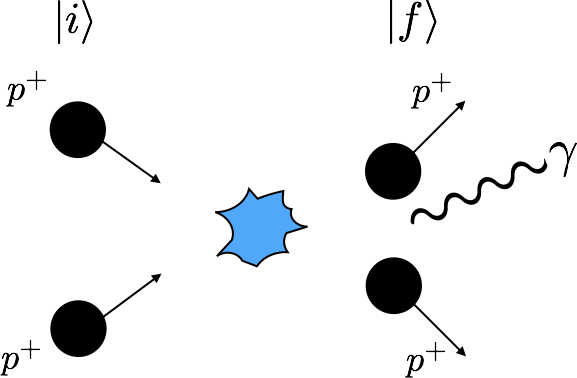
\includegraphics[width=.55\linewidth]{figures/QFT/istate_fstate.png}
\caption{An example of an initial state $\ket{i}$ with two incoming protons and a final state $\ket{f}$ with two outgoing protons and a photon $\gamma$. The blue object represents the interaction that takes place during the collision.}
\label{fig:ifstates}
\end{figure}
 The probability that the system evolves from state $\ket{i}$ into $\ket{f}$ is equal to the squared modulus of the amplitude,
\begin{equation}
\pif=|{\rm M}_{fi}|^{2},
\label{eq:Amp}
\end{equation}
and is in fact the only observation about a theory that can be made in physics experiments. After an initial and a final state are chosen, $\pif$ can be computed for a given QFT hypothesis and compared to the $\pif$ observed in experiment, and, depending on the consistency of the two answers, evidence can begin to build for or against the hypothesis. Commonly, $\pif$ is computed for two or more competing hypotheses, and the degree of consistency between each hypothesis and the experimental result are compared. In this way, a given hypothesis may be ``favored by the data'' relative to some other hypothesis, an idea that is further discussed in Chapter \ref{chap:run1pmssm}. Clearly, having a way to predict amplitudes is of utmost experimental importance. However, since most physicists are ultimately interested in understanding the physics that underlies the amplitude calculation\textemdash in other words, the physics that describes nature more deeply\textemdash a bit more detail is called for.


\section{Fields}

The primary degrees of freedom of a QFT are the fields. Mathematically, fields are single- or vector-valued functions of the spacetime coordinates, time and position in space. Physically, fields are interpreted as invisible objects that fill  space, taking on a density that varies from point to point, and sometimes an associated direction that likewise varies from point to point (Fig. \ref{fig:field}). A field can carry any number of properties, including energy, momentum, angular momentum, and charge density. When two or more fields interact, the relative local densities of the fields undergo changes, which can result in the the exertion of forces or the creation of matter.
\begin{figure}[h]
\centering
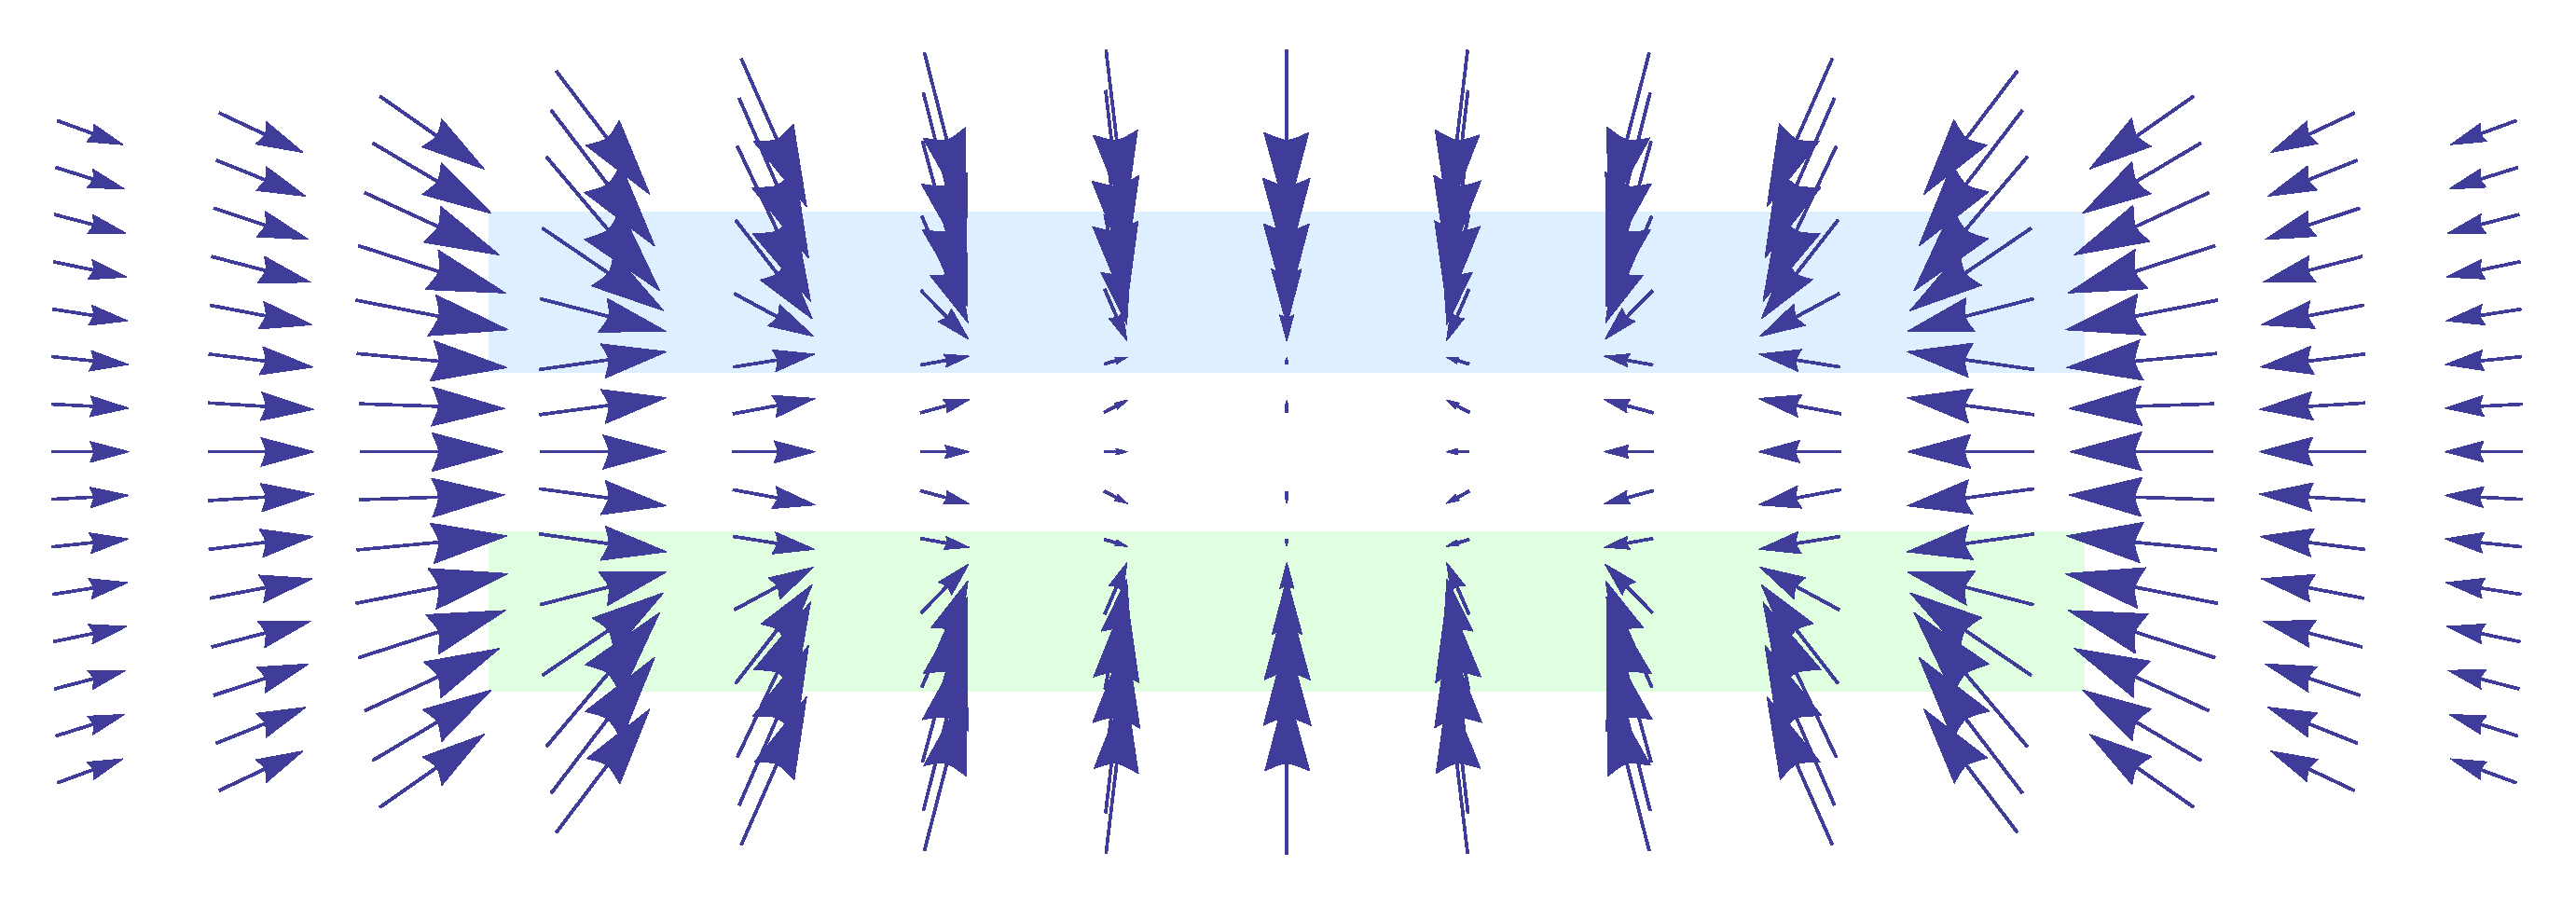
\includegraphics[width=.95\linewidth]{figures/QFT/GField.pdf}
\caption{An example of a field. The dark blue arrows show the magnitude and direction of the gravity field between two massive parallel plates shown in light blue and green. }
\label{fig:field}
\end{figure}

\section{Symmetry}
The way fields interact with one another depends on the set of symmetries that are present in the theory. Here, a symmetry is a property that ensures that some aspect of a system remains unchanged when the system is transformed in some way. Certain symmetries are inherent in every QFT, and these are the 10 non-spin related spacetime symmetries corresponding to the 10 generators of the Poincar{\'e} group~\cite{Peskin:1995ev}: 3 spatial translations and 1 time translation, 3 rotations,  and 3 boosts. Here, boosts are the generators of the Lorentz group, transforming a system from one inertial reference frame to another. All of these transformations correspond to invariant quantities, giving rise to the laws of the conservation of momentum, energy, angular momentum, and of the spacetime interval defined in special relativity. 

Other symmetries are referred to as internal or ``gauge" symmetries, and are free to be chosen during the construction of a QFT. An example of a gauge symmetry is the so-called unitary-1, or U(1), symmetry, which is respected by objects that do not change when they undergo planar rotations. In an abstract geometrical sense, circles respect U(1) symmetry because their shapes do not change when they are rotated about their centers by any angle; in the sense of a gauge symmetry, U(1) is notably respected by the QFT known as quantum electrodynamics (QED), the first successful QFT, because QED contains a parameter which, if rotated about the complex unit circle, yields back the same theory. 

The transformation of a field under a given symmetry can be represented by an operator $\hat{T}$, which is an object that changes (operates) on another object. The transformation on a field $\phi$ can be written as
\begin{equation}
\hat{T}[\phi] = \phi',
\end{equation}
where $\phi$ is the original field and $\phi'$ is the transformed field. The criterion for a theory to be invariant under a transformation $\hat{T}$ is that the Lagrangian density be unchanged after the replacement of the old fields by the transformed fields.

\section{Lagrangian density}
\label{sss:QFT}
 The mathematical object that encodes all the information in a perturbative (well-behaved) QFT is the Lagrangian density $\Lag$, sometimes just called the Lagrangian. The Lagrangian is a measure of the potential energy of a system subtracted from the kinetic energy, and is composed of terms proportional to the products of the field densities. The exact form of $\Lag$ follows from the set of fields and symmetries that are chosen in the QFT, and the various terms contain information about different physical processes. As an example, we examine the Lagrangian for a QFT in which there is only one field $\phi$, which is single valued (a scalar) and real. The Lagrangian density for this theory is given by
 \begin{equation}
 \Lag =  \frac{1}{2}(\partial_\mu \phi)^2  - a\phi^2 - b\phi^4,
 \label{eq:exLag}
 \end{equation} 
where a and b are constants and $\partial$ is the partial derivative taken with respect to the spatial coordinates. It is apparent that this Lagrangian is an expansion in powers of the field, and this is a general feature of Lagrangians; they are in fact Taylor expansions in the fields. 

The concept of symmetry can be illuminated in the context of this Lagrangian, because $\Lag$ can be seen to respect a particular symmetry called $\ztwo$ symmetry. $\ztwo$ symmetry is the invariance of a system under the operation of reversing the sign of the fields. In other words, a Lagrangian that respects a $\ztwo$ symmetry is invariant under the operation of $\hat{T}$, where $\hat{T}$ is defined by 
\begin{equation}
\hat{T}[\phi] \equiv \phi' = -\phi.
\end{equation}
All terms in this Lagrangian contain even powers of the field $\phi$, and so all minus signs brought about by the operation of $\hat{T}$ on $\Lag$ cancel, giving back the original Lagrangian:
 \begin{align}
 \begin{split}
\hat{T}[\Lag] \equiv \Lag' &= -\frac{1}{2}\partial_\mu (-\phi) \partial^\mu (-\phi)  - a(-\phi)^2 - b(\phi)^4 \\
&= -\frac{1}{2}\partial_\mu \phi \partial^\mu \phi  - a\phi^2 - b\phi^4 \\
&= \Lag.
 \label{eq:exLag2}
  \end{split}
\end{align} 
If $\Lag$ had contained a term proportional to $\phi^3$, the theory would not respect a $\ztwo$ symmetry, because $\hat{T}[\Lag]$ would not yield back $\Lag$.

As stated, each term in the Lagrangian carries specific physical meaning. The first term in Equation \ref{eq:exLag} accounts for the kinetic energy stored in the field, the second term accounts for particle mass, and the third term is an interaction term. These points are discussed now.

\section{Particles (quadratic term)}
A field typically exhibits a resonance at an energy value proportional to the coefficient of the quadratic term in the Lagrangian; in this case, twice the value of a. This resonance is referred to as a particle, and has a mass defined by the energy of the resonance:
\begin{equation}
m_{\phi} = 2a.
\end{equation}
Particles are localized quanta, or pieces, of the fields, and they carry the same properties as the fields. These properties include energy $E$ and momentum components $p_i$ ($i=x,y,z$), which can be combined into a single object called a four-vector,
\begin{equation} 
p^\mu=(E,p_x,p_y,p_z)^\mu,
\end{equation}
whose magnitude is invariant under Lorentz transformations; particles can also carry charge, a property that is invariant under gauge transformations; and they have spin, where spin is the ``intrinsic'' angular momentum possessed by a particle in the absence any interaction taking place. The smallest natural increment of spin is equal to half of Planck's constant $\hbar$, and thus all particles have a spin equal to an integer multiplied by this unit:
\begin{equation}
s_\phi = N\cdot \frac{\hbar}{2}.
\end{equation}
Particles for which $N$ is an even integer are called bosons, and those with an odd $N$ are called fermions. The bosonic or fermionic nature of particles in a system determines many bulk properties of the system, most importantly whether or not the particles can be arranged to form rigid structures; fermions are able to do so, and bosons are not.
%Whether a particle is a boson or a fermion determines many properties about that particle, including notably whether it can occupy %don't think I need this

\section{Feynman diagrams (interaction terms)}
\label{sec:withztwo}
As mentioned in Section \ref{sec:Amp}, the primary role of QFT from an experimental point of view is to predict amplitudes. To a first approximation, the amplitude for a system to evolve from state $\ket{i}$ to state $\ket{f}$ is given by the quantity
\begin{equation}
{\rm M}_{fi}=\bra{f}\hat{H}\ket{i},
\end{equation}
where the time evolution operator $\hat{H}$ can be derived from the Lagrangian. 
%In this expression, $\hat{H}$ acts on and modifies the state $\ket{i}$, the resulting state is projected onto the final state $\ket{f}$, and this yields the amplitude. % maybe won't need
There are various methods for computing this amplitude, but the most widely used is Feynman's method. Feynman's method amounts to doing a perturbative expansion over the possible ways (modes) for the state $\ket{i}$ to transform into state $\ket{f}$. Each possible mode is weighted by a number that can be computed from a diagram, and after the partial amplitudes for all possible diagrams have been computed, they are added together to form the amplitude M$_{fi}$. By Equation \ref{eq:Amp} the square of the amplitude yields the probability for state $\ket{i}$ to evolve into state $\ket{f}$.

\begin{figure}[h]
\centering
%\hspace{0cm}f
\subfloat[allowed]{
  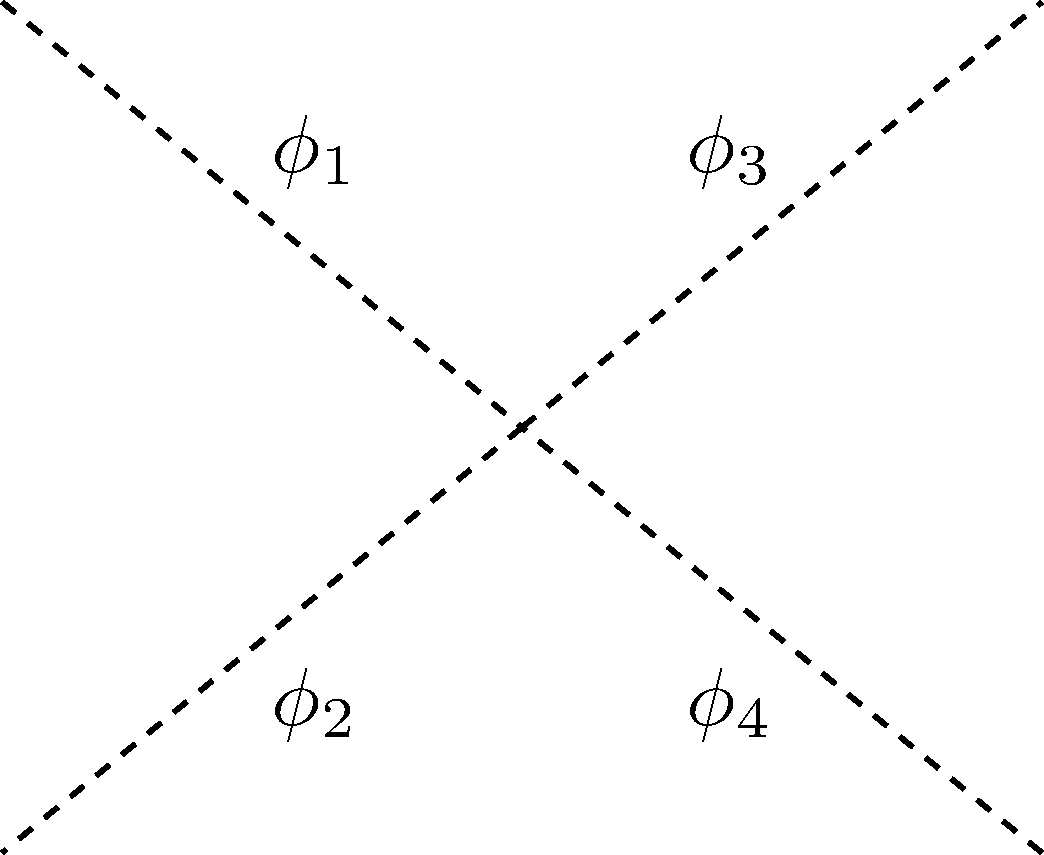
\includegraphics[width=0.32\linewidth]{figures/QFT/feyn1}
}
%\hspace{1cm}
\subfloat[allowed]{
  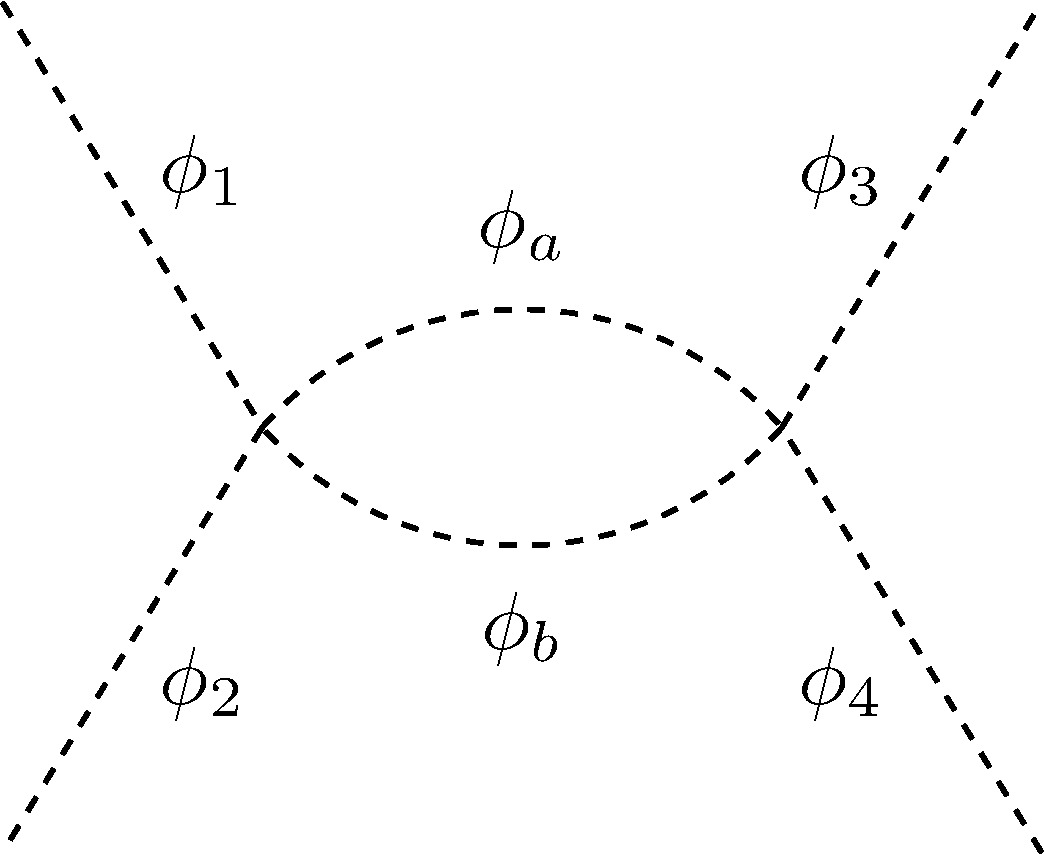
\includegraphics[width=0.32\linewidth]{figures/QFT/feyn2}
}
%\\
\subfloat[forbidden before SSB]{
  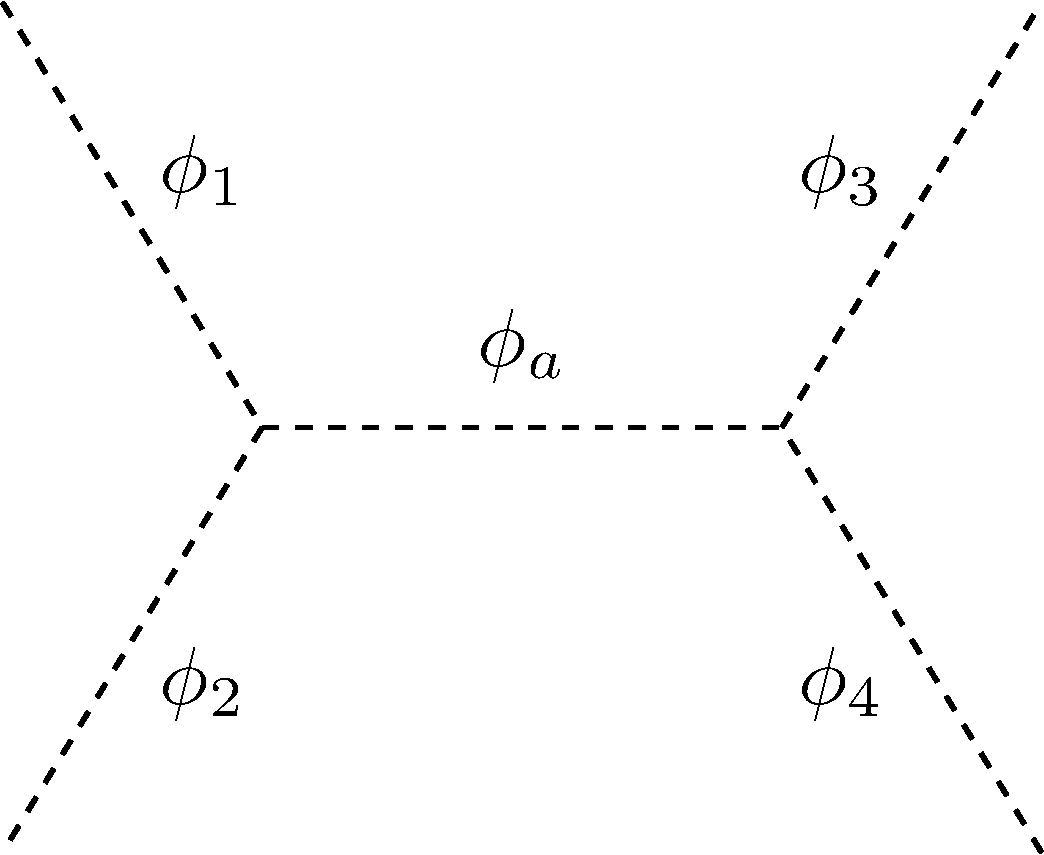
\includegraphics[width=0.32\linewidth]{figures/QFT/feyn3}
}
\caption{Diagrams a and b are two of the leading Feynman diagrams in the theory defined by Equation \ref{eq:exLag}. Diagram c is forbidden by the theory, and so does not contribute to the amplitude. }
\label{fig:Feyn}
\end{figure}

Suppose, for example, we are working within the theory defined by the Lagrangian in Equation \ref{eq:exLag}, that the initial state $\ket{i}$ consists of two identical incoming particles $\phi_1$ and $\phi_2$, and that the final state $\ket{f}$ consists of two outgoing particles $\phi_3$ and $\phi_4$. Figure \ref{fig:Feyn} 
shows two of the leading Feynman diagrams (a and b), each representing a possible mode for the specified process, and one diagram c that is not allowed by the theory. Each allowed diagram contributes a partial amplitude, and the sum of all partial amplitudes is the total amplitude M$_{fi}$. The two essential features of these and any Feynman diagrams are:
\begin{itemize}
\item lines, which represent particles of the field $\phi$, where dashes signify that in this case the particles have no spin, and
\item vertices, which are the fundamental interactions between particles.  
\end{itemize}
By convention, time flows horizontally, and so the initial state consists of the particles on the left side of a diagram, and the final state consists of the particles on the right side. Diagrams a and c are called tree level diagrams because they appear to have branches that do not close to form loops. Diagram b, by contrast, contains an internal loop of particles, and so is not a tree-level diagram. Tree-level diagrams typically yield the largest partial amplitudes, and thus are often the most important.

The guiding principle for constructing diagrams is that any diagram not forbidden by the theory will, in principal, contribute to the total amplitude. Allowed diagrams are those for which every vertex within a diagram is associated with a term in the Lagrangian. For our $\Lag$, the only interaction term is the quartic term, $c\phi^4$, and this term gives rise to the four-particle vertex seen in the center of the diagram in Fig. \ref{fig:Feyn} (a). This can be generalized, since a term in a Lagrangian proportional to n powers of a field gives rise to an n-particle vertex in the theory. The more complicated diagram in Fig. \ref{fig:Feyn} (b) is built out of two copies of the four-particle vertex, and so is allowed. One could imagine a vertex of only three $\phi$ particles, shown in Fig. \ref{fig:Feyn} c. However, the three-particle vertex does not correspond to any term in the Lagrangian. For such a vertex to exist, $\Lag$ would have to contain a term proportional to $\phi^3$, and it was already established that such a term would violate the $\ztwo$ symmetry respected by the theory. Therefore, the three-particle vertex, and diagram c, are forbidden by symmetry, and so do not enter into the amplitude calculation. 

In principle, one should construct and compute all possible diagrams and amplitudes, of which there are an infinite number, but this turns out to be unnecessary if the goal is to make reasonably accurate predictions. The simplest diagrams\textemdash the tree-level diagrams\textemdash typically give the largest contribution to the amplitude because they have fewer vertices than do more complicated diagrams. Each vertex contributes a factor of $4!\cdot b$ to the partial amplitude, and provided that $4!\cdot b$ is always less than 1,  diagrams with more vertices yield smaller partial amplitudes. Taking an approximation where only the tree-level diagrams (diagram a) contribute, the amplitude and probability are given by\footnote{For a complete description of the Feynman rules, see \cite{Peskin:1995ev}.}:
\begin{align}
%\begin{split}
&{\rm M}_{fi}=-(4!)\ b,\\
&\pif = (-4!)^2\ b^2 = 576\ b^2.
%\end{split}
\end{align}
The quantity $(4!)b$ is sometimes referred to as a coupling constant, $\lambda$, named so because its value dictates the strength of the amplitude associated with the interaction. A couple of observations: first, the amplitude contains a single power of the constant b, because the contributing diagram has only a single vertex. Second, a notable feature of the probability is that $\pif$ is constant with respect to all kinematic properties of the outgoing particles. This means that if many collisions were to occur in succession, the distribution of the final state particles would be isotropic. Of course, this is a conclusion reached by analyzing the leading order contributions. If diagram b or other higher-order diagrams had been included, the prediction of isotropic final states might not have been absolute, but any deviation from this behavior would be suppressed by additional factors of b. 

\section{Conserved quantities}
Noether's theorem \cite{Noether:1918zz} states that every continuous symmetry respected by a theory is associated with some conserved quantity, and the same is often true in the case of discrete symmetries. It was established that the QFT at hand respects a $\ztwo$ symmetry, so what is the associated conserved quantity? The answer can be deduced through a bit of analysis of the interaction terms of the Lagrangian. In $\Lag$, terms with an even number of powers of the field are present, which means that vertices involving an even number of particles are allowed. However, terms with odd powers of the fields are not present, which means that vertices with an odd number of particles are not allowed. This fact means that while it is possible for a pair of particles to be created or destroyed, the same is not true for a single particle. If the initial number of particles is even, the final number will also be even; if the initial number is odd, the final number will be odd. The conserved quantity is:
\begin{equation}
\theta = n\pmod{2},
\label{eq:theta}
\end{equation}
where $n$ is the number of particles in the system. In this theory, the value of $\theta$ for an isolated system can never change.

\section{Symmetry breaking}
The previous analysis of the scalar Lagrangian was valid but not unique. It was assumed that the parameters $a$ and $b$ were positive, but it happens that the dynamics of the theory change considerably if the parameter $a$ takes on a negative value. Since the Lagrangian is constructed as the difference between the kinetic and potential energy of the system, the second and third term define a potential energy V:
\begin{equation}
V(\phi) = a\phi^2 + b\phi^4.
\end{equation}
For positive $a$, $V(\phi)$ exhibits a minimum at the value $\phi=0$, as seen in Fig. \ref{fig:SSB} (a) and (b). But if $a$ is negative, $V(\phi)$ exhibits two minima, located at 
\begin{equation}
\phi_{min} \equiv {\rm VEV} = \pm \sqrt{\frac{a}{2b}},
\end{equation}
where VEV is the vacuum expectation value, that is, the average value of the field in the vacuum.
\begin{figure}[h]
\centering
\hspace{-0.3cm}
\subfloat[$a>0$]{
  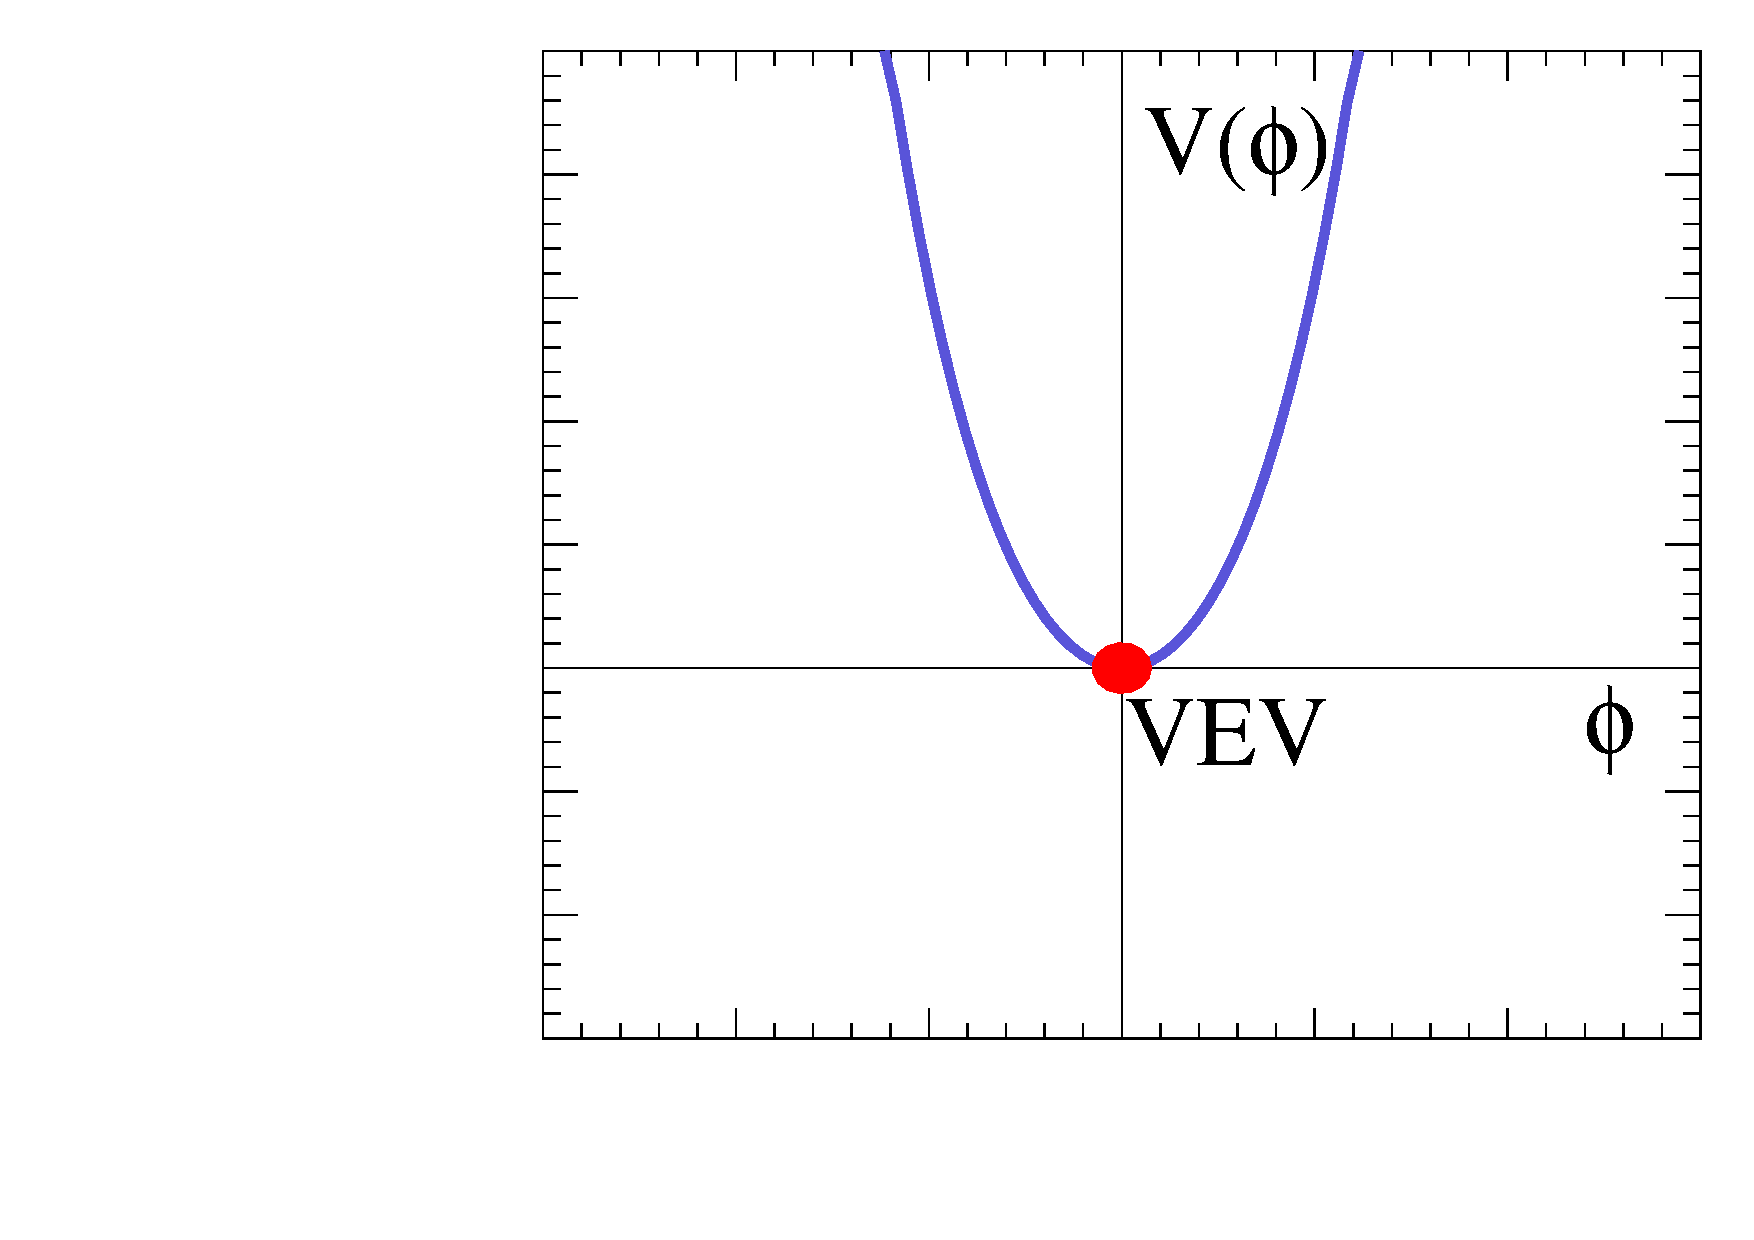
\includegraphics[width=0.33\linewidth]{figures/QFT/SB1.pdf}
}
\hspace{-0.3cm}
\subfloat[$a=0$]{
  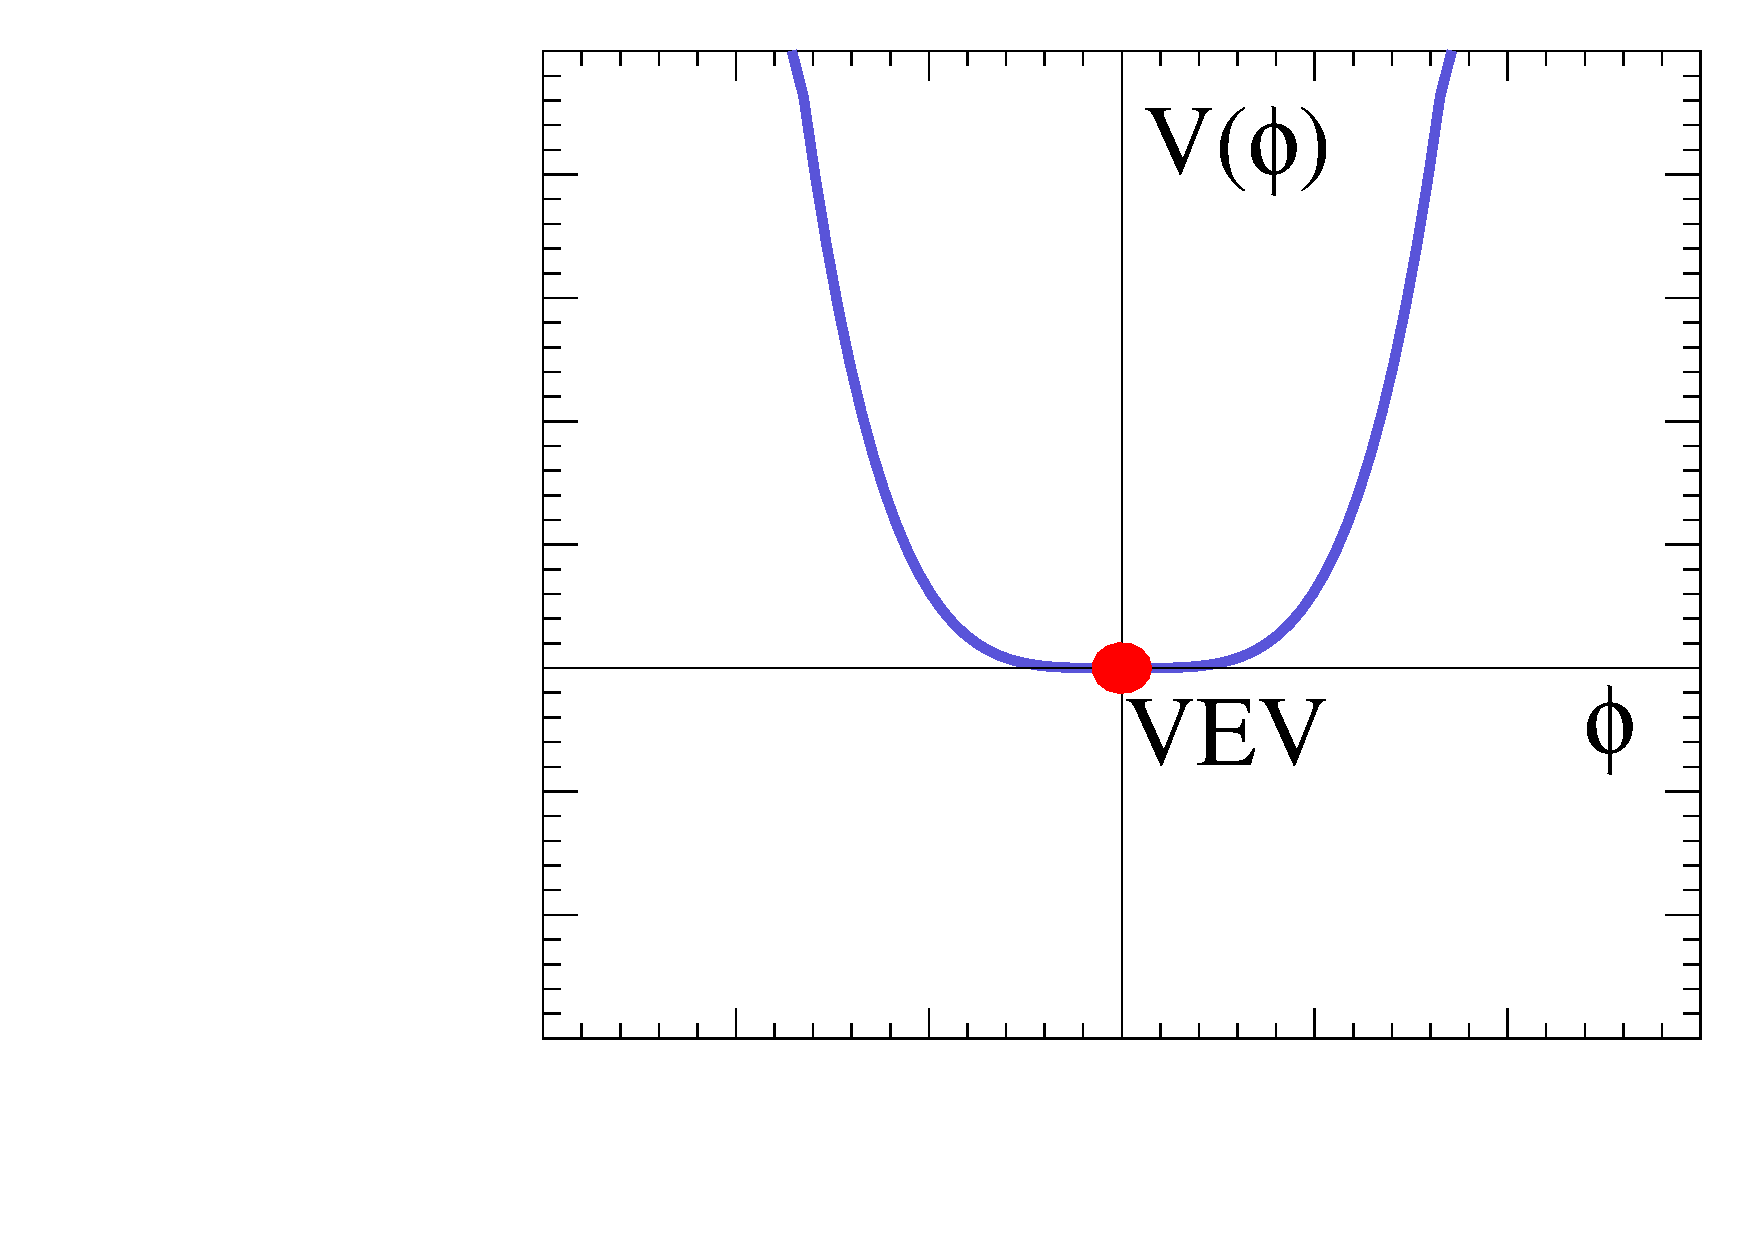
\includegraphics[width=0.33\linewidth]{figures/QFT/SB2.pdf}
}
\hspace{-0.3cm}
\subfloat[$a<0$]{
  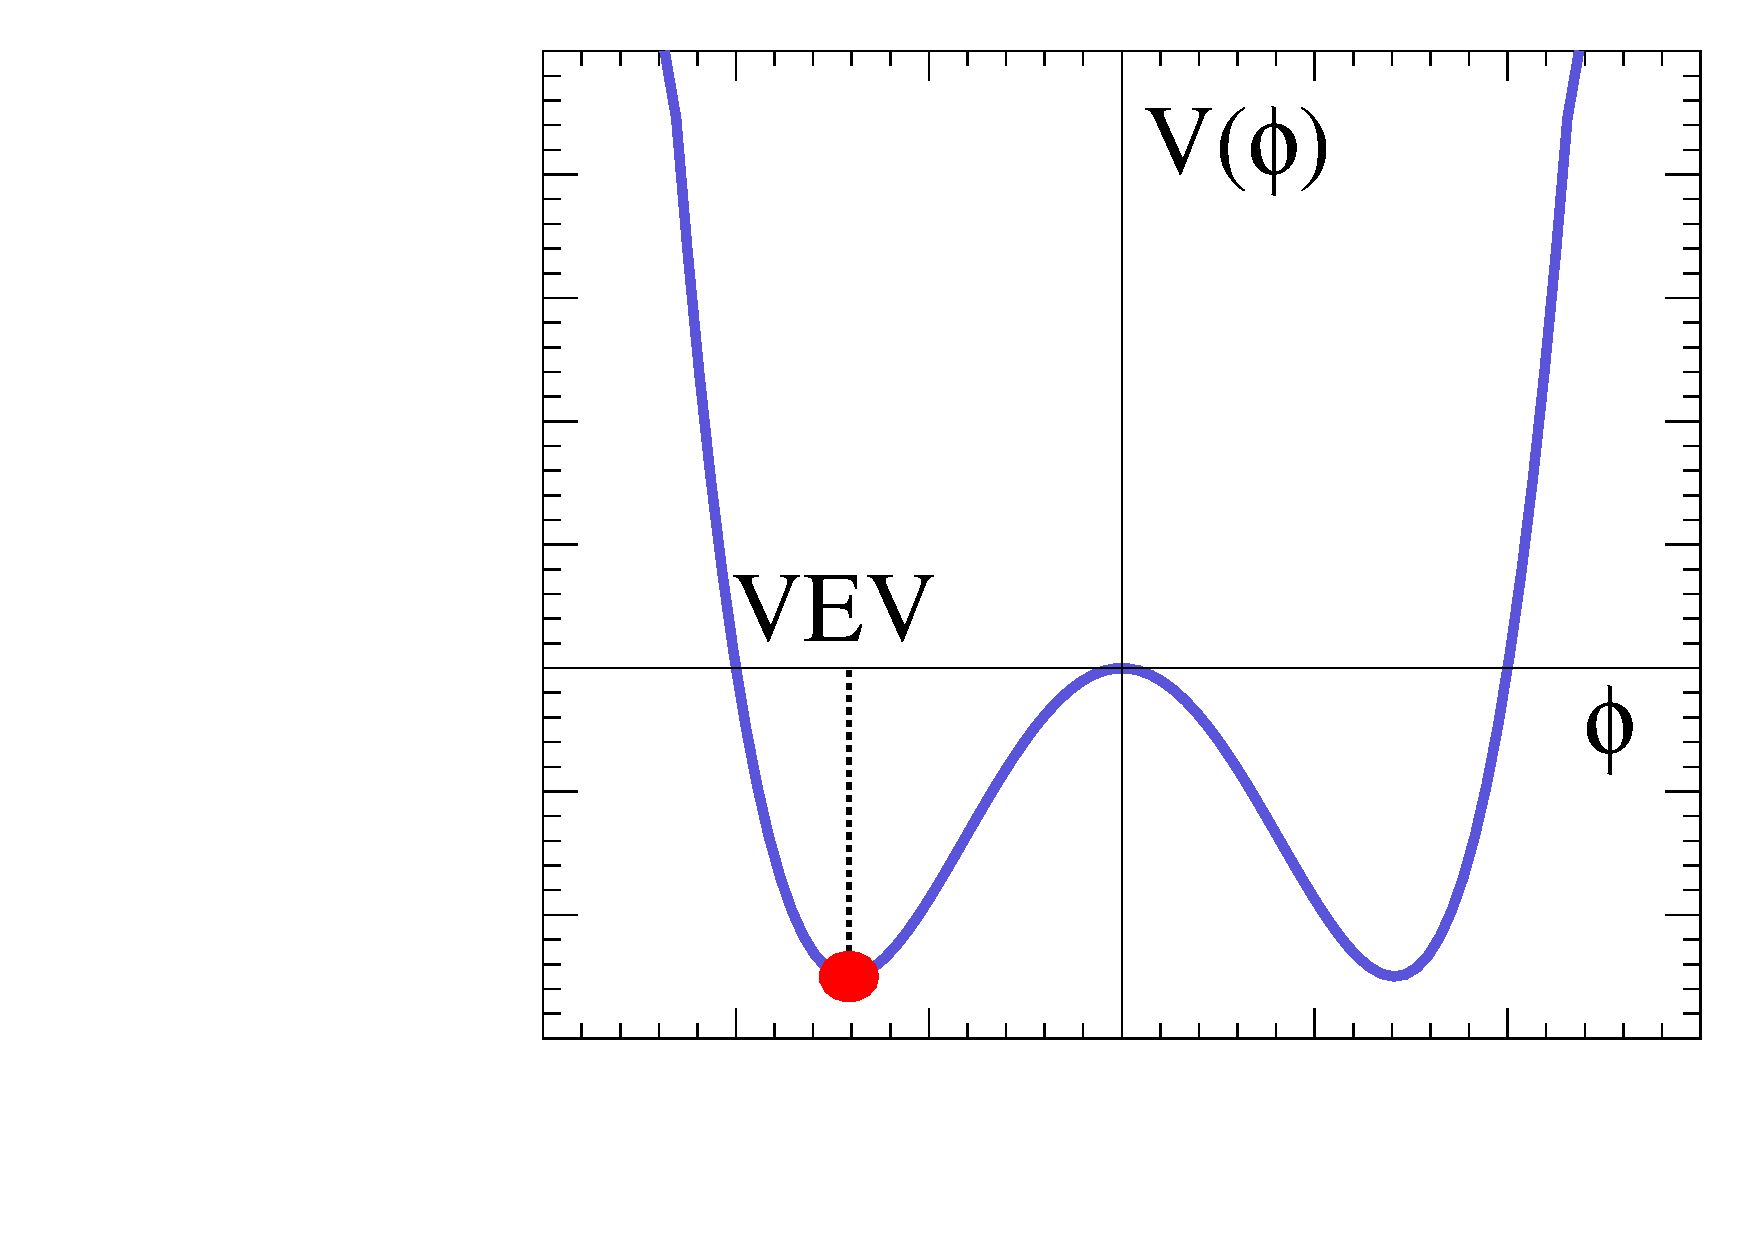
\includegraphics[width=0.33\linewidth]{figures/QFT/SB3.pdf}
}
\caption{The shape of the potential for three choices of parameter a: positive, zero, and negative. The field $\phi$ always centers on a local minimum of the potential, which is marked in the three cases by the red dot. }
\label{fig:SSB}
\end{figure}

Physical systems tend to evolve towards a state of lower energy, and so it is no surprise that the appearance of these energy minima leads to a qualitative change in the behavior of the system.  The field density will naturally settle into one of these minima, located at an energy value equal to the VEV. When this happens, a visible change takes place at the level of the Lagrangian. The field $\phi$ splits into a static component equal to the VEV, and a dynamic part, which is the modified field $\phitwo$:
\begin{equation}
\phi \rightarrow {\rm VEV}+\phitwo.
\end{equation}
The Lagrangian in Equation \ref{eq:exLag} becomes
\begin{align}
\begin{split}
\Lag \rightarrow& -\frac{1}{2}(\partial_\mu [{\rm VEV}+\phitwo])^2  - a[{\rm VEV}+\phitwo]^2 - b[{\rm VEV}+\phitwo]^4\\
 = &\ \frac{1}{2}(\partial_\mu \phitwo)^2 - (a {\rm VEV}^2 + b {\rm VEV}^4) - (2 a {\rm VEV} + 4 b {\rm VEV}^3) \phitwo \\
& \ \ \ \ \ \ \ \ \ \ \ \ \ \ \ \ \  - (a + 6 b {\rm VEV}^2) \phitwo^2 - 4 b {\rm VEV} \phitwo^3 - b \phitwo^4 
\equiv \Lag_{\rm broken}.
 \end{split}
\end{align}
The terms without any powers of $\phitwo$ are non-physical and so can be ignored, and through a renaming of the constants, the Lagrangian can be written as
\begin{equation}
\Lag_{\rm broken} = \frac{1}{2}(\partial_\mu \phitwo)^2 - \alpha \phitwo^2 - \gamma \phitwo^3 - \beta \phitwo^4.
\end{equation}
Note that $\Lag_{\rm broken}$ closely resembles the original Lagrangian $\Lag$, but differs in a few key ways. For one, the coefficients of the quadratic and quartic terms have changed from $a$ and $b$ to $\alpha$ and $\beta$, where the latter depend on the magnitude of the symmetry breaking (the VEV). This means that the mass and coupling strength of the four-particle vertex have changed, which will ultimately result in a re-scaling of $\pif$. 

Then, the fact that there is now a cubic term ($\gamma \phitwo^3$) is particularly significant. In $\Lag$, the cubic term was explicitly forbidden by the $\ztwo$ symmetry, but upon the introduction of a non-zero VEV, $\ztwo$ is no longer respected. The symmetry is said to have been ``spontaneously broken.''  As a result of the emergent cubic term, the theory has a new allowed vertex of three particles, and so the interaction in the diagram of Fig. \ref{fig:Feyn} c is no longer forbidden! This changes the prediction for the amplitude, which now has four contributing tree-level diagrams instead of just one. The probability now depends on the the kinematics of the particles, and so the outgoing particles will no longer be distributed isotropically. Clearly, symmetry breaking has changed the physics considerably.

Perhaps the most striking change brought about by the breaking of the $\ztwo$ symmetry is that the previously conserved quantity $\theta$ (in Equation \ref{eq:theta}) is no longer conserved. Through processes involving the new three-particle vertex, the system can now start out with an even number of particles and end up with an odd number, or vice versa. Indeed, symmetry breaking is seen to have fundamentally changed the physics.

The concept of spontaneous symmetry breaking (SSB) is particularly relevant for the $\SM$ because it is key to the mechanism by which all the particles in the $\SM$ acquire mass, known as the Brout-Englert-Higgs mechanism \cite{Higgs:1964pj}. Before proceeding to describe the $\SM$, there is one last concept that must be mentioned, and that is of commutation relations.

\section{Commutation relations}
Symmetries are defined by an invariance under the action of an operator, and operators are defined by a set of commutation relations. In other words, they are defined by how they transform the states they act on, and by how they behave when applied in sequence with other operators. In general, the commutator and anticommutator of two operators $\hat{T}_1$ and $\hat{T}_2$ are defined by
\begin{align}
[\hat{T}_1,\hat{T}_2]\phi &\equiv \hat{T}_1 (\hat{T}_2 \phi)  - \hat{T}_2 (\hat{T}_1 \phi) \text{\ and}\\
\{\hat{T}_1,\hat{T}_2\}\phi &\equiv \hat{T}_1 (\hat{T}_2 \phi)  + \hat{T}_2 (\hat{T}_1 \phi),
\end{align}
respectively. Broadly speaking, boson fields commute, meaning their commutators are equal to 0, and fermion fields anticommute, meaning their anticommutators are equal to 0. For more information on commutators and QFT, please see Ref.~\cite{Peskin:1995ev}.

The reader has now received an entertaining yet strategic introduction to the basic concepts and vocabulary that will be necessary to describe the $\sm$ and what seems to be the endless search for supersymmetry.




\chapter{The Standard Model}
\label{chap:SM}
The standard model (SM) is the quantum field theory that describes the fundamental fields and symmetries observed in nature thus far.  These fields, artistically represented in Figure \ref{fig:SMcircle}, and symmetries are discussed here. 
\begin{figure}[h]
\centering
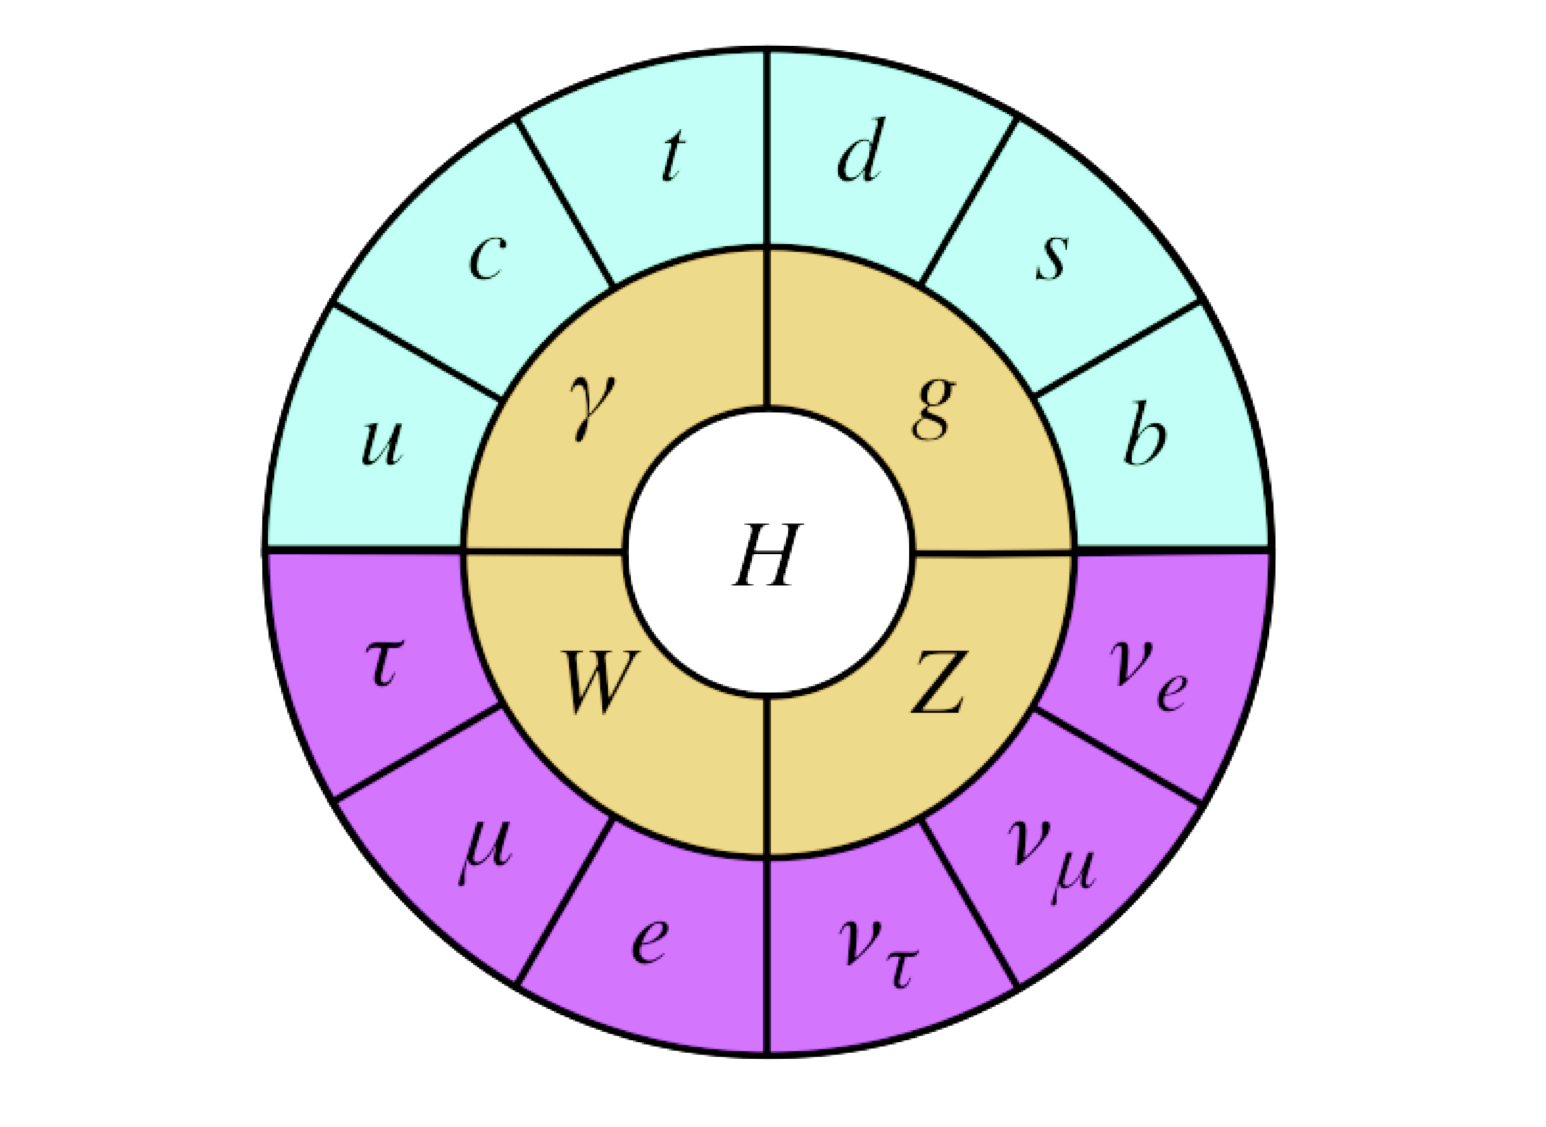
\includegraphics[width=.6\linewidth]{figures/SM/StandardModel2.png}
\caption{The fields of the standard model. From inside out, concentric annuli represent the spin-0, spin-1, and spin-$\frac{1}{2}$ fields.}
\label{fig:SMcircle}
\end{figure}

\section{SM fields and symmetries}
Like all QFTs, the standard model is symmetric under transformations of the 10 non-spin related spacetime degrees of freedom, which map to the 10 generators of the Poincare group. 

In addition to the usual spacetime symmetries, the standard model exhibits invariance under transformations of three gauge groups, each group being associated with a set of massless spin-1 (vector) fields:
\begin{itemize}
\item the circle group $\uone$, whose transformation can be represented by a unitary scalar operator (complex one) multiplied by a charge called the weak hypercharge Y. The associated vector field is called ${\rm B}_{\mu}$;
\item the $n=2$ special unitary group $\sutwo$, whose three transformations can be represented by the $2\times2$ Pauli matrices $\sigma_{i}$ ($i=1,2,3$) multiplied by a charge called the weak isospin $T_3$. The three associated vector fields are $W_{\mu}^{1,2,3}$;
\item the $n=3$ special unitary group $\suthree$, whose eight operations can be represented by the $3\times3$ Gell-Mann matrices $\lambda^{j}$ ($j=1,...,8$) multiplied by a charge called the color $C=(r,g,b)$. The eight associated vector fields are $G_{\mu}^{1,...,8}$.
\end{itemize}
In total, that makes 12 vector fields associated with three gauge symmetries, all of which can be summarized by the tensor product of groups that defines the gauge symmetry of the standard model:
\begin{equation}
\uone \cross \sutwo \cross \suthree.
\label{eq:symm}
\end{equation}
The standard model also has 12 spin-1/2 (fermion) fields $\psi$, sometimes referred to as ``matter fields,'' 6 of which are the lepton fields and 6 are quark fields.  Of the lepton fields, there are three charged fields, electron (e$^-$), muon ($\mu^-$), and tau ($\tau^-$), and three neutral fields, electron neutrino ($\nu_{\rm e}$), muon neutrino ($\nu_{\mu}$), and tau neutrino ($\nu_{\tau}$). Of the quark fields, there are three ``up-type'' fields, up (u), charm (c), and top (t), and three ``down-type'' fields, down (d), strange (s), and bottom (b). Fermions contain a property called chirality, and they can either be left-chiral, or right-chiral, which are sometimes referred to as left- or right- handed. For mysterious but experimentally verified reasons, left-handed fermion fields transform differently under the SU(2)$_{\rm L}$ gauge symmetry than do the right-handed fermion fields, which results in an asymmetry in the properties of fermions; specifically, there are left-handed and right-handed charged leptons, left-handed neutrinos, but no right-handed neutrinos.

The last field in the standard model is a complex scalar doublet field ($\phi$), named the Higgs field after one of the theorists who predicted its existence in 1964 \cite{Higgs:1964pj}. 

\section{SM Lagrangian}
The standard model Lagrangian \cite{Langacker:1995hi} can be written in a somewhat simplified form as
\begin{align}
\begin{split}
\Lag_{\rm SM} =& \frac{1}{2}(\partial_\mu \phi)^2 
- \frac{1}{2}\mu^2\phi^{2}
-\frac{\lambda}{4}\phi^{4}
+\frac{1}{4}g_{1}^{2}({\rm B}_{\mu})^2\phi^2 + \frac{1}{4}\sum_{i=1}^{3}g_{2}^2 (\sigma^{i} {\rm W}^{i}_{\mu})^2\phi^2 \\
&+ \sum_{i,j=1}^{9}\psi_i y_{ij} \psi_{j}\phi
+\sum_{i=1}^{8}\frac{1}{4}\bigg[\partial_\mu {\rm G}^{i}_\nu - \partial_\nu {\rm G}^{i}_\mu - \sum_{j,k=1}^{8}g_s f_{ijk} {\rm G}^{j}_{\mu}{\rm G}^{k}_{\nu}\bigg]^2
+\Lag_{\rm gauge, kin}.
\end{split}
\end{align}
The first three terms are much like the $\phi^4$ scalar Lagrangian introduced in Section \ref{sss:QFT}, except for one trivial and one non-trivial difference. The trivial difference is that the names of the coefficients on $\phi^2$ and $\phi^4$ have been tweaked slightly to reflect their true meaning (the scalar mass and a coupling constant, respectively), and the non-trivial difference is that the field $\phi$ is now a complex scalar doublet rather than a real-valued number, and so $\phi^2\equiv\phi^{\dag}\phi$, where $^\dag$ denotes hermitian conjugation. The fourth and fifth term are determined from invariance under the $\uone\cross\sutwo$ (electroweak) symmetry and are the allowed interactions of the W and B vector fields with the scalar field, where $g_{1}$ and $g_{2}$ are coupling constants. The sixth term features a sum over all pairs of charged fermion fields, and amounts to the set of allowed interaction terms between the fermion fields and the scalar; the constants $y_{ij}$ are called Yukawa couplings. The seventh term defines the properties of the gluon fields, where $g_s$ is the strong coupling constant and $f_{ijk}$ are so-called structure constants determined by the SU(3) symmetry group. The final term, $\Lag_{\rm gauge, kin}$ includes terms for the kinetic energy of fermion and gauge boson fields and a few higher-order interaction terms, but is not essential for this discussion.

\section{Electroweak symmetry breaking}

One conspicuous feature of this Lagrangian is the absence of any mass terms apart from the scalar mass term. The symmetry in Expression \ref{eq:symm} actually forbids quadratic terms for either the fermion or gauge boson fields, and so one might expect this model to describe a system which does not contain massive particles\textemdash certainly not our universe. However, as with the unbroken $\phi^4$ theory described earlier, this Lagrangian does not explicitly reveal all the dynamics. The coefficient of the quadratic term (in this case $\mu^2$) is measured to be negative, and this causes the scalar potential $V(\phi)$ to exhibit a minimum value at
\begin{equation}
|\phi|_{min}={\rm VEV}=\sqrt{\frac{-\mu^2}{\lambda}}.
\end{equation}
The universe is thought to have long ago slipped into the ground state with $\phi$ centered on the vacuum expectation value VEV. In this case, the Lagrangian can be re-expressed in terms of the fields through the replacement
\begin{align*}
\phi\rightarrow {\rm VEV} + {\rm h}, 
\end{align*}
where VEV acts as a constant and h is the new dynamic field, the Higgs field. The above replacement yields a Lagrangian that no longer respects the $\uone\cross\sutwo$ symmetry:
\begin{align}
\setlength{\jot}{25pt}
\abovedisplayskip=-20pt
\belowdisplayskip=-20pt
\vp \Lag_{\rm SM} \rightarrow\  & \Lag_{\rm SM}'
\nonumber \\\vp 
\Lag_{\rm SM}'=& \frac{1}{2}(\partial_\mu [{\rm VEV}+{\rm h}])^2 
- \frac{1}{2}\mu^2[{\rm VEV}+{\rm h}]^{2}
-\frac{\lambda}{4}[{\rm VEV}+{\rm h}]^{4}
\nonumber \\\vp 
+&\frac{1}{4}g_{1}^{2}({\rm B}_{\mu})^2[{\rm VEV}+{\rm h}]^2 + \frac{1}{4}\sum_{i=1}^{3}g_{2}^2 (\sigma^{i} {\rm W}^{i}_{\mu})^2[{\rm h}+{\rm \vp \vp VEV}]^2 
\nonumber \\\vp +& \sum_{i,j=1}^{9}\psi_i y_{ij} \psi_{j}[{\rm VEV}+{\rm h}]
+\sum_{i=1}^{8}\frac{1}{4}\bigg[\partial_\mu {\rm G}^{i}_\nu 
- \partial_\nu {\rm G}^{i}_\mu - \sum_{j,k=1}^{8}g_s f_{ijk} {\rm G}^{j}_{\mu}{\rm G}^{k}_{\nu}\bigg]^2
\nonumber \\\vp 
+&\Lag_{\rm gauge, kin}, %%%
\end{align}
\begin{align}
\hphantom{\Lag_{\rm SM}'=}=&\frac{1}{2}(\partial_\mu {\rm h})^2 
+ \frac{1}{2}\mu^2 {\rm h}^{2}
- \lambda{\rm VEV}{\rm h}^{3} 
- \frac{\lambda}{4}{\rm h}^{4}
+  {\color{blue} \frac{1}{4}g_{1}^{2}{\rm VEV}^2({\rm B}_{\mu})^2}
\nonumber \\\vp
+ &\frac{1}{2}g_{1}^{2}{\rm VEV}({\rm B}_{\mu})^2{\rm h}
+ \frac{1}{4}g_{1}^{2}({\rm B}_{\mu})^2{\rm h}^2 
+ {\color{blue}\frac{1}{4}g_{2}^2{\rm VEV}^2\sum_{i=1}^{3}(\sigma^{i} {\rm W}^{i}_{\mu})^2)}
\nonumber \\\vp
+ & \frac{1}{2}g_{2}^2 {\rm VEV}\sum_{i=1}^{3}(\sigma^{i} {\rm W}^{i}_{\mu})^2{\rm h}^2
+ \frac{1}{4}g_{2}^2\sum_{i=1}^{3}(\sigma^{i} {\rm W}^{i}_{\mu})^2{\rm h}^4
+ \sum_{i,j=1}^{9}\psi_i y_{ij} \psi_{j}{\rm h}
\nonumber \\\vp 
+ & {\color{blue}({\rm VEV})\hspace{-.1cm}\sum_{i,j=1}^{9}\psi_i y_{ij} \psi_{j}}
+ \frac{1}{4}\sum_{i=1}^{8}\bigg[\partial_\mu {\rm G}^{i}_\nu - \partial_\nu {\rm G}^{i}_\mu - \sum_{j,k=1}^{8}g_s f_{ijk} {\rm G}^{j}_{\mu}{\rm G}^{k}_{\nu}\bigg]^2 
\nonumber \\\vp 
+ &\Lag_{\rm gauge, kin}.
\end{align}
The terms highlighted in blue are quadratic in the fields and indicate that several standard model particles have ``acquired'' mass through their interactions with the Higgs field. The third blue term indicates that the 9 charged standard model fermions each now have an associated mass equal to the VEV multiplied by their respective Yukawa coupling. Similarly, the first and second blue terms show that the gauge fields B and W are associated with masses as well; the electroweak symmetry has been spontaneously broken. Note that there are still no terms quadratic in the gluon fields G, and so the gluons remain massless; the $\suthree$ symmetry remains unbroken. We are left with a model that more closely resembles $\nature$, but there is one stone left unturned. It is known that nature retains one massless electroweak gauge boson, the photon $\gamma$, and so it must be that one of the $\EW$ field terms has a quadratic term equal to zero. This is achieved through a mixing of the B and W fields, wherein new fields are defined as various combinations of the old fields:
\begin{align}
\vps W_{\mu}^{+} =& \frac{1}{\sqrt{2}}(W_{\mu}^1 - i W_{\mu}^2)\\
\vps W_{\mu}^{-} =& \frac{1}{\sqrt{2}}(W_{\mu}^1 + i W_{\mu}^2)\\
\vps Z_{\mu} =& -{\rm sin}\theta_{W}{\rm B}_\mu+{\rm cos}\theta_{W}W_{\mu}^3\\
\vps A_{\mu} =&+{\rm cos}\theta_{W}{\rm B}_\mu+{\rm sin}\theta_{W}W_{\mu}^3,
\end{align}
where $\theta_W$ is the electroweak mixing angle (the Weinberg angle), defined as:
\begin{equation}
\theta_{W}={\rm tan}^{-1}(g_1/g_2).
\end{equation}
The new gauge fields are associated with masses equal to
\begin{align}
\vps m_{W} &= \frac{1}{2}{\rm VEV}g_{2}, \\
\vps m_{Z} &= \frac{1}{2}{\rm VEV}\sqrt{g_{1}^{2}+g_{2}^{2}},\\
\vps m_{A} &= 0.
\end{align}
The massless field $A_{\mu}$ is identified as the electromagnetic field, or the photon field. This field respects a new U(1) symmetry, the symmetry of electromagnetism, ${\rm U(1)}_{\rm EM}$, whose generator of transformations is the well-known electric charge $Q=T_3+\frac{1}{2}Y$. It is said that the electroweak symmetry breaks to the electromagnetic symmetry:
\begin{equation}
\uone\cross\sutwo\cross\suthree\rightarrow{\rm U(1)}_{\rm EM}\cross\suthree
\end{equation}

\section{SM parameters and visualization}
\label{sec:parcor}
A summary of the standard model fields and particles is given in Table \ref{tab:SM}.  
\begin{table}[h]
\begin{centering}
\caption{The fields and particles of the $\SM$ and their quantum numbers. The gluon color can take on eight unique combinations of $c_i\bar{c}_j$ ($i,j=1,2,3$) where $c_1=r\ {\rm (red)},c_2=g\ {\rm (green)}, {\rm and }\ c_3=b\ {\rm (blue)}$.}
\makebox[\textwidth][c]{
\begin{tabular}{ l | l | c | c | c | c | c | c}
\hline
\hline
name & fields & spin & ${\rm Y}$ & ${\rm T}_3$ & Q & C & mass states \\
\hline
\hline
fermion &&&&&&& \\
%\multicolumn{7}{l}{fermion}&\\
\hline
\hline
\multirow{2}{*}{charged} & $e_L$, $e_R$ & \multirow{12}{*}{$\frac{1}{2}$}&\multirow{3}{*}{$-1, -2$}&\multirow{3}{*}{$-\frac{1}{2}, 0$}&\multirow{3}{*}{$-1$}&\multirow{6}{*}{$0$}&$e^{-}$\\
\cline{2-2}\cline{8-8}
\multirow{2}{*}{lepton}&$\mu_L$, $\mu_R$&&&&&&$\mu^{-}$\\
\cline{2-2}\cline{8-8}
&$\tau_L$, $\tau_R$&&&&&$$&$\tau^{-}$\\
\cline{1-2}\cline{4-6}\cline{8-8}
\multirow{3}{*}{neutrino} & $\nu_{\rm eL},-$ &&\multirow{3}{*}{$-1,-$}&\multirow{3}{*}{$+\frac{1}{2},-$}&\multirow{3}{*}{$0,-$}&&\multirow{3}{*}{$\nu_1, \nu_2, \nu_3$}\\
&$\nu_{\mu L},-$ &&&&&&\\
&$\nu_{\tau L},-$ &&&&&&\\
\cline{1-2}\cline{4-8}
\multirow{2}{*}{up-type}&$u_L$, $u_R$ &&\multirow{3}{*}{$+\frac{1}{3}, +\frac{4}{3}$}&\multirow{3}{*}{$+\frac{1}{2},0$}&\multirow{3}{*}{$+\frac{2}{3}$}&\multirow{3}{*}{$r,g,b$}&\\
\cline{2-2}
\multirow{2}{*}{quark}&$c_L$, $t_R$&&&&&&\multirow{2}{*}{hadrons}\\
\cline{2-2}
&$t_L$, $t_R$&&&&&&\multirow{2}{*}{(baryons}\\
\cline{1-2}\cline{4-7}
\multirow{2}{*}{down-type}&$d_L$, $d_R$ &&\multirow{3}{*}{$+\frac{1}{3}, -\frac{2}{3}$}&\multirow{3}{*}{$-\frac{1}{2},0$}&\multirow{3}{*}{$-\frac{1}{3}$}&\multirow{3}{*}{$r,g,b$}&\multirow{2}{*}{\& mesons)}\\
\multirow{2}{*}{quark}&$s_L$, $s_R$&&&&&&\\
&$b_L$, $b_R$&&&&&&\\
\hline
\hline
boson&&&&&&&\\
%\multicolumn{7}{l}{boson}&\\
\hline
\hline
Higgs&H&$0$&$1$&$-\frac{1}{2}$&0&$0$&h\T\B\\
\hline
B boson&B&\multirow{5}{*}{1}&$0$&$0$&$0$&$0$&\multirow{2}{*}{$\gamma$, $Z$}\T\B\\
\cline{1-2}\cline{4-7}
\multirow{3}{*}{W boson} & ${\rm W}^{3}$ &&$0$&$0$&$0$&$0$&\T\B\\
\cline{2-2}\cline{4-8}
&${\rm W}^{2}$ &&$0$&$+1({\rm W}^{+})$&$+1({\rm W}^{+})$&$0$&\multirow{2}{*}{${\rm W}^{+}$, ${\rm W}^{-}$}\T\B\\
\cline{2-2}\cline{7-7}
&${\rm W}^{1}$ &&$0$&$-1({\rm W}^{-})$&$-1({\rm W}^{-})$&$0$&\T\B\\
\cline{1-2}\cline{4-8}
gluon&${\rm G}^{1,...,8}$&&$0$&$0$&0&$c_i \bar{c}_j$&glueballs\T\B\\
\hline
\hline
\end{tabular}
}
\label{tab:SM}
\end{centering}
\end{table}
In total, the standard model has 19 free parameters, all of which have been measured. They are
\begin{itemize}
\item{9 fermion mass parameters, one for each charged fermion;}
\item{1 Higgs mass parameter $m_h$ (the Higgs boson was discovered and $m_h$ measured in 2012 \cite{Chatrchyan:2012xdj}); 
\item 1 vacuum expectation value, the VEV;}
\item{3 field strength constants, $g_1$, $g_2$, and $g_3$}; and
\item{5 additional mixing parameters appearing in $\Lag_{\rm gauge, kin}$ not discussed herein: $\theta_{12}$, $\theta_{23}$, and $\theta_{13}$, $\delta$, and $\theta_{\rm QCD}$.}
\end{itemize}

The values of these parameters can be represented using the technique of parallel coordinates visualization~\cite{bib:parcor}. In a parallel coordinates plot, independent variables are represented by vertical parallel axes, and points in the hyperspace spanned by the independent variables are represented by horizontal lines traversing the plot from left to right. In Figure \ref{fig:parcorSM}, the standard model is represented as the red line, intersecting each axis at the value of the parameter assumed by the theory, in this case the measured value.  

The information in Equation \ref{eq:symm}, Table \ref{tab:SM}, and Figure \ref{fig:parcorSM} fully defines the standard model.

\begin{sidewaysfigure}[tb!]
\begin{centering}
\makebox[\textwidth][c]{
\hspace{-.5cm}
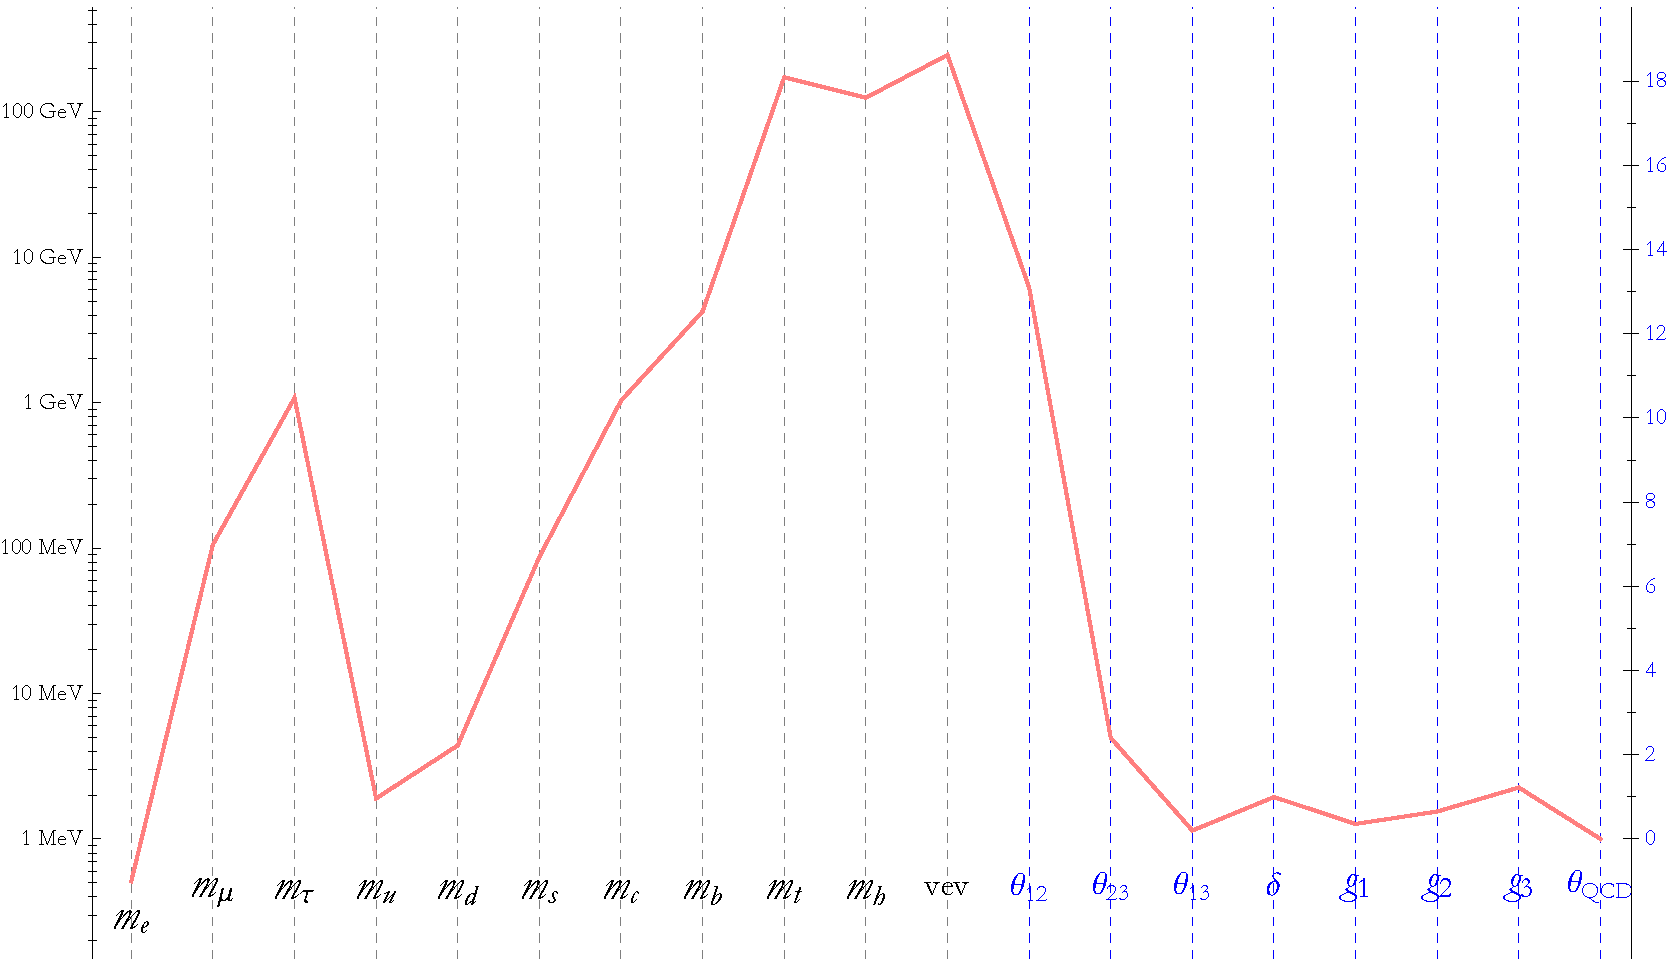
\includegraphics[width=1.0\linewidth]{figures/parallel_coordinates/ParCorSM.pdf}
}
\caption{A parallel coordinates plot of the 19 standard model parameters. Values on the black axes have dimensions of energy and are read from the left, while the values on the blue axes are read from the right.}
\label{fig:parcorSM}
\end{centering}
\end{sidewaysfigure}

%\section{Problems with the standard model}
\label{sec:problems}
As stated earlier, there are three reasons why the standard model is believed not to provide a full explanation of all natural phenomena. The first pertains to certain observations that seem to directly contradict predictions of the standard model. The second is the behavior seen in some systems that, while not directly contradicting the predictions of the standard model, seem to go beyond the standard model's ability to account for them. And finally, there is the puzzling observation that the standard model contains a high degree of fine tuning.  While the second issue is of much importance, it is not directly relevant to this work, and so further discussion is left to the literature. However, the following is a discussion of the first and last issue.

\subsection{Observations in tension with the standard model}
The most striking shortcoming of the standard model is that it lacks a description for gravity.  Gravity was the first force to be fully understood over large distances, but it will likely be the last to be fully understood at very short distances. This is because the force of gravity is very weak, as it carries a coupling constant that is $10^{34}$ times smaller than the electromagnetic coupling $\alpha$. Gravitational effects would not be observable in particle collisions below a center of mass energy close to the Planck scale ($10^{19}$ GeV), mindbendingly larger than the energetic reach of modern particle colliders. Most theoretical models that could describe the standard model and gravity, sometimes called theories of everything or ultraviolet (UV) completion models, manifest new phenomena only above a large energy called $\cutoff$, roughly in the vicinity of the Planck scale. 

Another observation not predicted by the standard model is that of neutrino mass.  The Higgs field does not interact with neutrinos because neutrinos are left-chiral and have no right-chiral counterparts (see Figure \ref{tab:SM}); neutrinos in the standard model are massless. However, neutrinos were recently observed to oscillate between flavors \cite{Fukuda:1998mi}, a behavior that is only possible if the neutrinos have mass. This seemingly innocuous observation is in fact quite profound, because it implies that some still unknown theory of particles, with masses of higher energy than the standard model, exists. A number of theories have emerged that could potentially explain neutrino mass, including the types I, II, and III seesaw mechanisms \cite{Yanagida:1980xy}, all of which predict heavy right-handed neutrinos whose mass is inversely proportional to the corresponding left-handed neutrino mass. If a lower bound on the masses of the standard model neutrinos were to be measured, this would specify the mass scale of the heavy neutrinos. Unfortunately, no lower bound has been established as yet, and so there are few clues about the nature of the true theory, or at what energy scale the phenomena of the new theory might be observable.

Another piece of evidence that suggests the standard model falls short of providing a full description of nature is the observation of dark matter in galaxies and in the intergalactic regions of the universe \cite{Davis:1985rj}\cite{Komatsu:2008hk}. Measurements of the baryonic mass of galaxies (the mass due to standard model particles) based on observed galactic luminosities are inconsistent with estimates of the total mass of galaxies based on rates of galactic rotation. The baryonic mass is, on average, a factor 6 lower than the total inferred mass, so it seems that there is a great deal of extra mass in galaxies not accounted for by the known particles.  
\begin{figure}[h]
\makebox[\textwidth][c]{
\centering
\subfloat[]{
  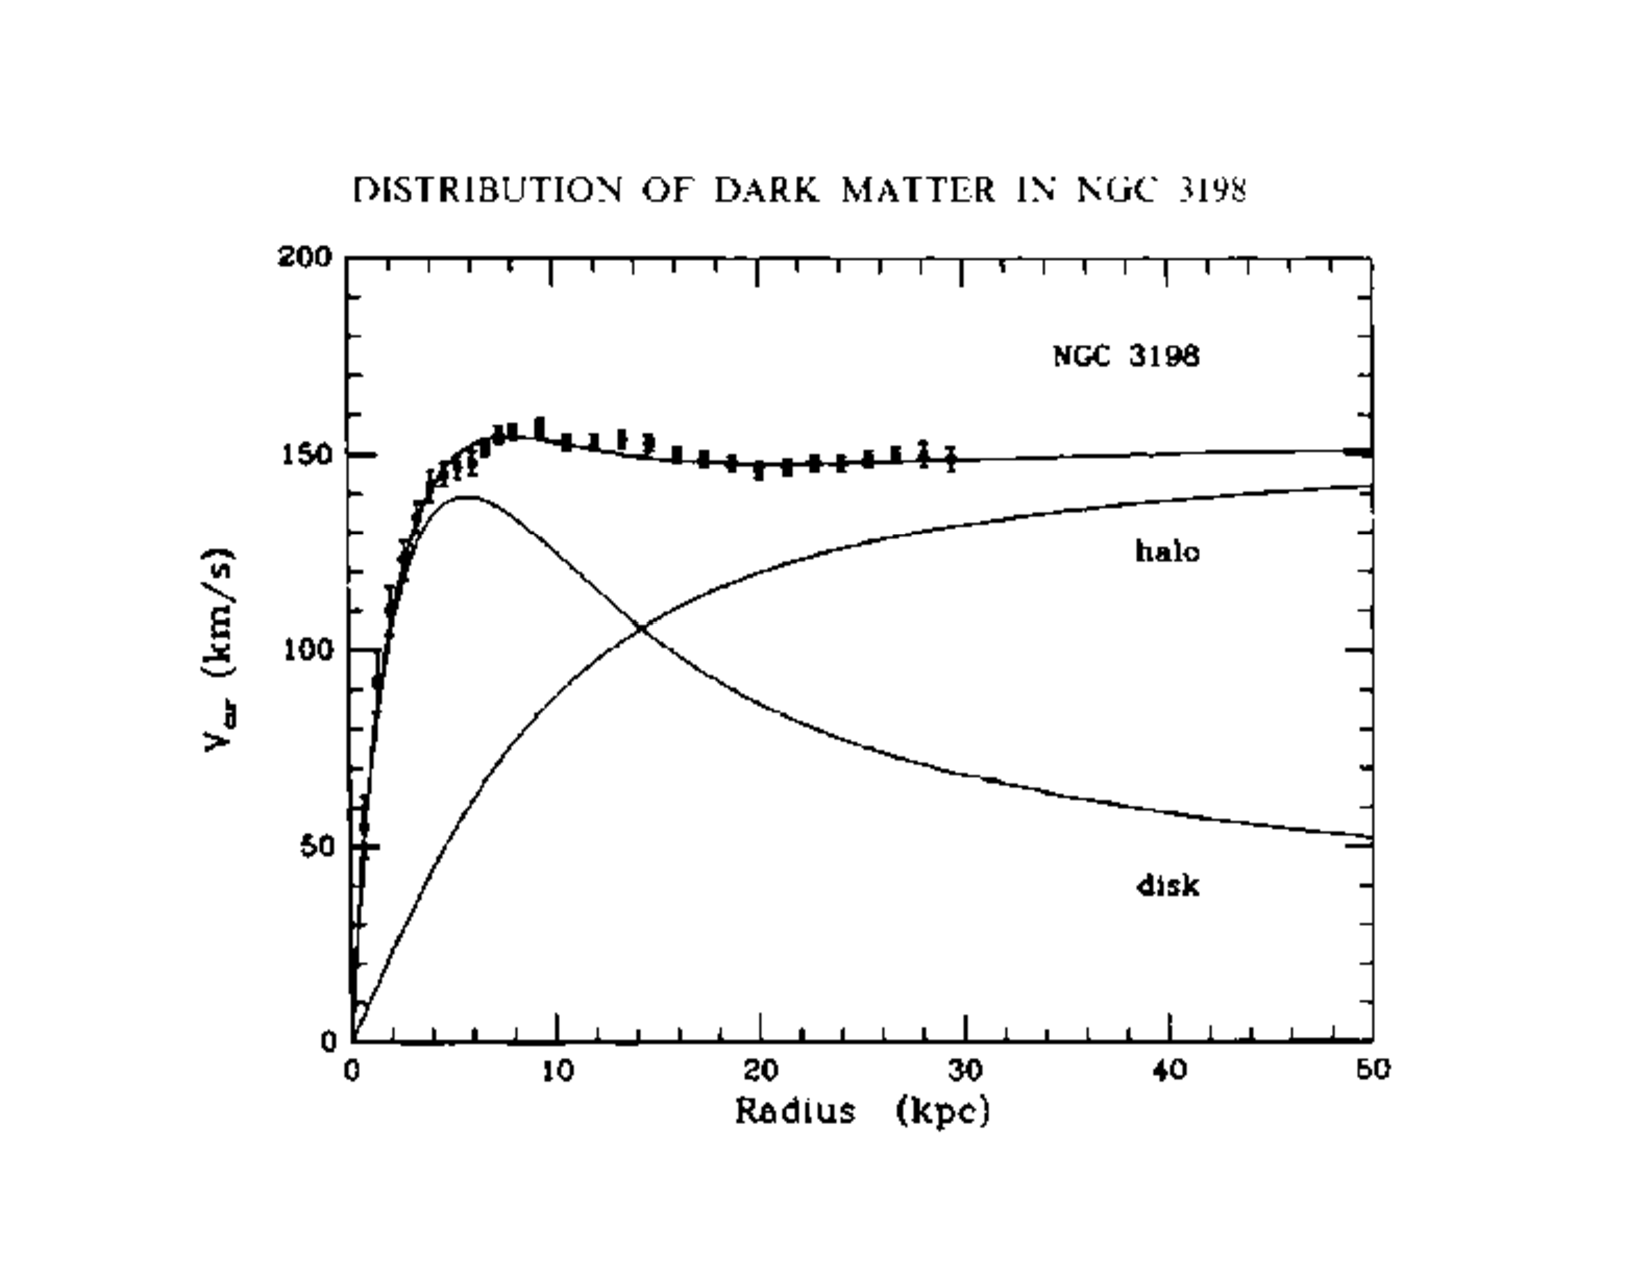
\includegraphics[width=0.6\linewidth]{figures/SM/NGC3198.pdf}
}
\hspace{-.2cm}
\subfloat[]{
  \vspace{2cm}
  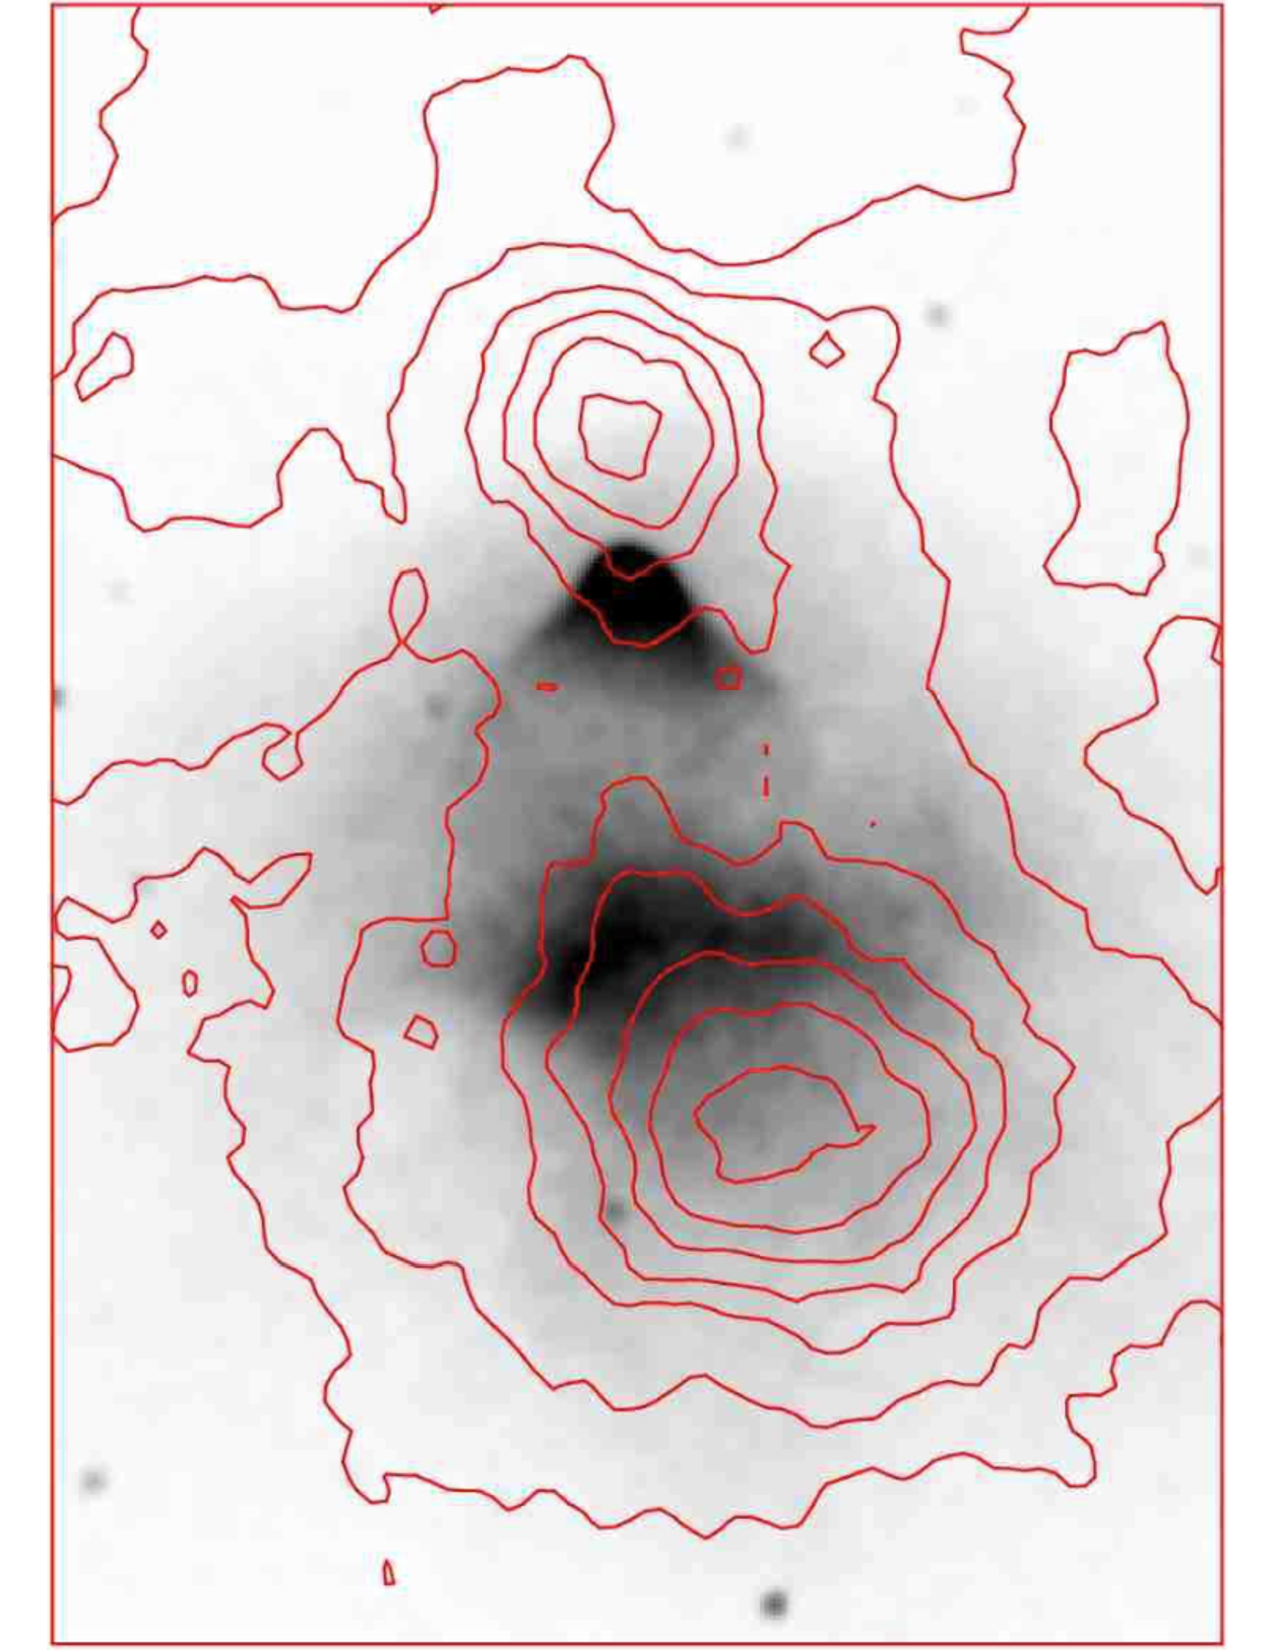
\includegraphics[width=0.46\linewidth]{figures/SM/DMConts.pdf}
}
}
\caption{Subfigure (a) \cite{vanAlbada:1984js} shows the orbital velocity of objects in galaxy NGC 3198 vs their distance from the galactic center. Subfigure (b) \cite{Clowe:2006xq} shows an X-ray photograph taken by the Chandra X-ray observatory of the aftermath of the collision of two galaxy clusters, 1E0657-558, overlaid on a contour map of the gravitation lensing magnitude factor $\kappa$ derived from a separate image taken by the Magellan 6.5 m telescope. } 
\label{fig:DM}
\end{figure}
The best-motivated explanation for this perceived excess is that some yet-undiscovered type of matter exists in abundance within galaxies, but doesn't emit or absorb light (and hence the moniker, ``dark matter''), and therefore has, at most, weak interactions. 

This inferred dark matter may come in the form of new particles, particles not described by the standard model, which may interact with the standard model particles at very high energy scales. This hypothesis is supported by observations of the speed of objects in galaxies as a function of their distance from the galactic center (see Fig. \ref{fig:DM} a). 
The expected speed of objects moving in the nearby galaxy NGC 3198 is given as a function of the orbital radius for the baryonic matter-only hypothesis (solid line peaking at 5 kpc), as well as for the  the baryonic matter+dark matter hypothesis (top solid line). The data (black points) show excellent agreement with the non-interacting dark matter hypothesis. Furthermore, it is claimed that direct evidence of dark matter is evident in the overlay in Figure \ref{fig:DM} (b), in which the aftermath of the collision of two galaxy clusters has been observed. The points of maximum baryonic matter density, represented in black, are displaced from the points of maximum total mass density as determined by the magnitude of gravitational lensing, indicated by the red contours. The interpretation is that the collision of the clusters caused the baryonic matter to collide and slow down, while the dark matter passed through the collision without slowing, resulting in the separation of the two populations of matter.

Dark matter may be discovered by direct or indirect detection experiments (see Ref.~\cite{Undagoitia:2015gya} for a review) or collider experiments like ATLAS \cite{Aad:2008zzm} and CMS \cite{Chatrchyan:2008aa}. A number of theories have been proposed as possible explanations of cosmological dark matter, including certain supersymmetric extensions of the standard model (discussed in Chapter \ref{chap:susy}).


Other observations requiring some explanation beyond the standard model include the fact that there is an abundance of matter in the cosmos but almost no anti-matter (baryon asymmetry), and the existence of the dark energy that accounts for the accelerating expansion of the universe \cite{Goldhaber:2009qu}.

\subsection{Fine tuning and unexplained patterns in the standard model}
\label{sec:finetune}
In a scientific context, tuning is the notion that the parameters of a model can either take on seemingly random values, or they can appear to follow some pattern. An un-tuned (or ``natural'') model refers to the former, and a highly-tuned (or fine-tuned) model refers to the latter. When an apparent pattern has been observed, centuries of science practice and common sense suggests that there should be a reason for the pattern. When a model seems to be fine-tuned, one of two possible, scientifically acceptable explanations must be the case:  
\begin{itemize}
\item{Either there are enough randomized versions (near copies) of the model that the chance emergence of such a pattern is a statistical inevitability; simultaneously, some kind of selection bias has lead the observer to examine the particular instance of the model that exhibited the pattern; or}
\item{there exists some mechanism that generates the observed pattern. }
\end{itemize}
For example, suppose you are shown a piece of toast with the pattern of a religious figure on the face, as in Figure \ref{fig:toast} (a) or (b). 
\begin{figure}[h]
\makebox[\textwidth][c]{
\centering
\subfloat[]{
  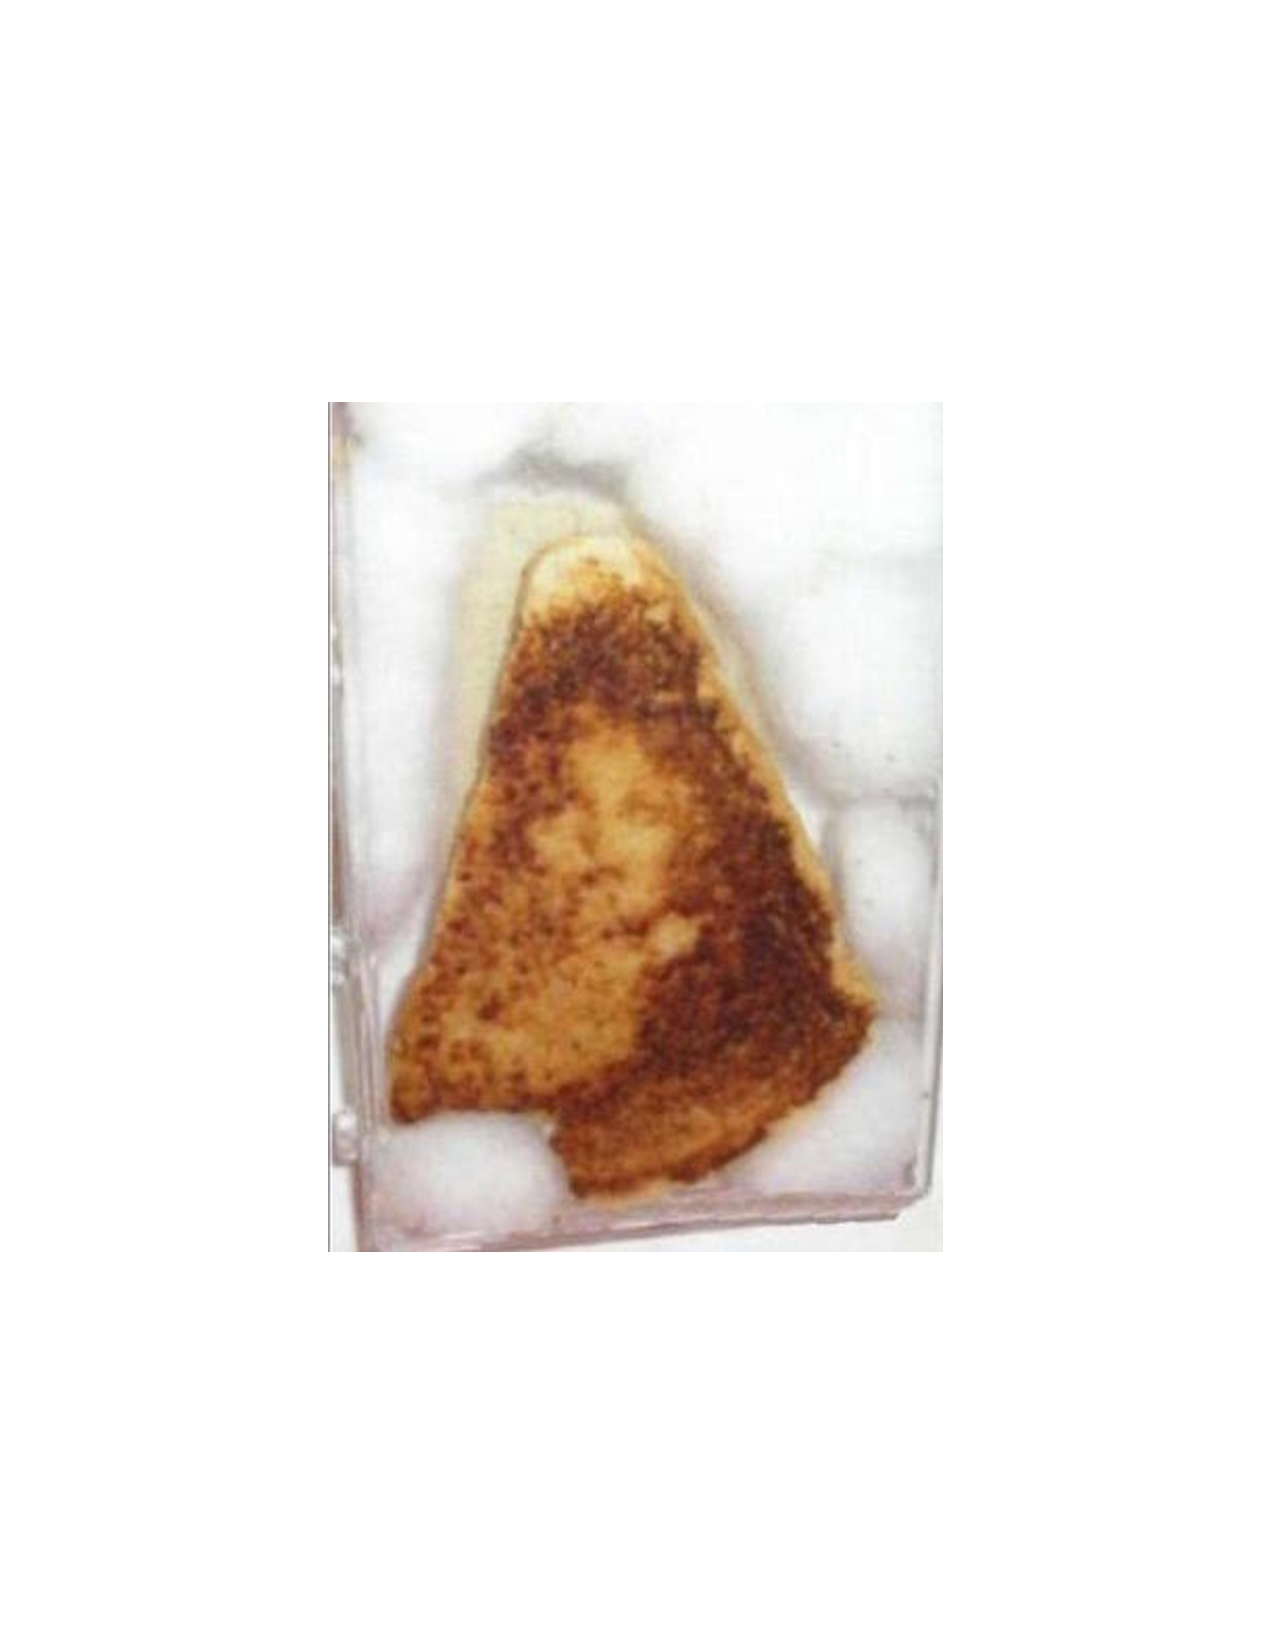
\includegraphics[width=0.3\linewidth]{figures/SM/Mary.pdf}
}
\hspace{-.2cm}
\subfloat[]{
  \vspace{2cm}
  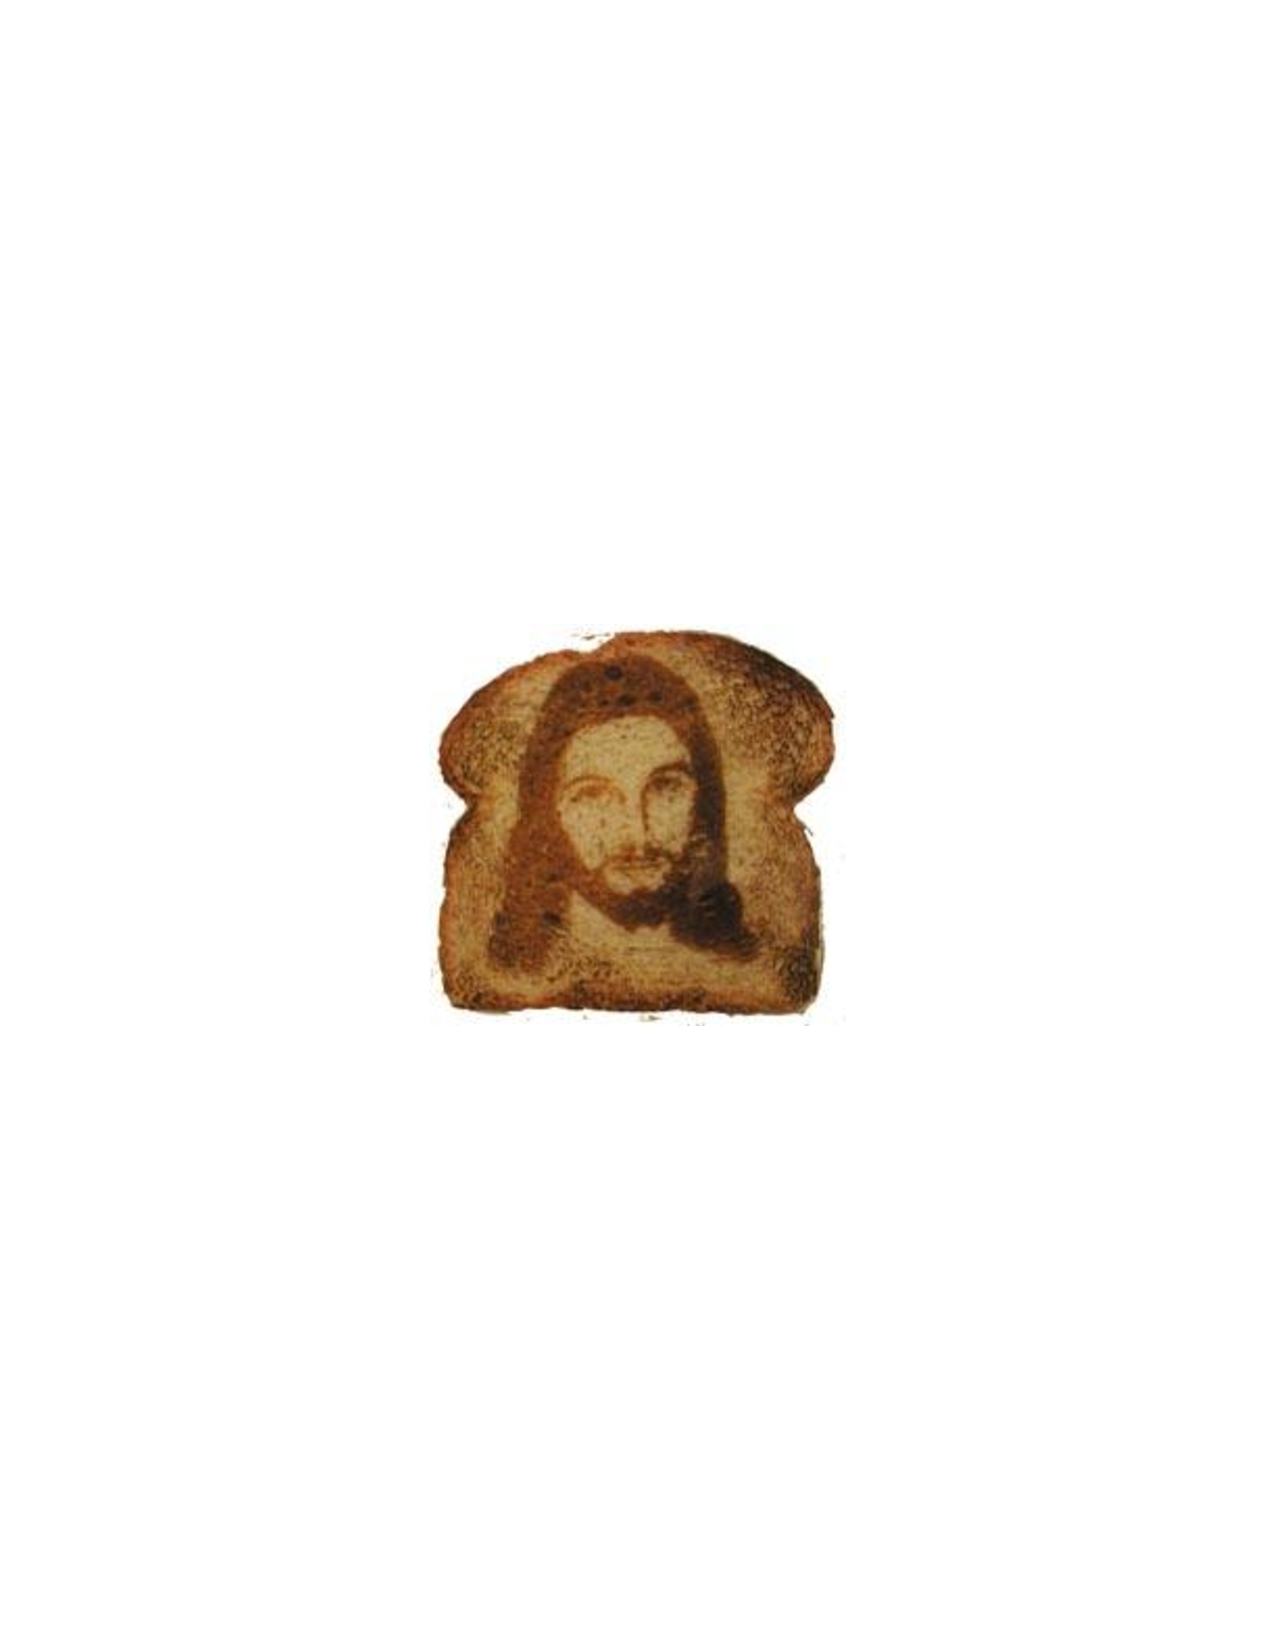
\includegraphics[width=0.33\linewidth]{figures/SM/Jesus.pdf}
}
\hspace{-.2cm}
\subfloat[]{
  \vspace{2cm}
  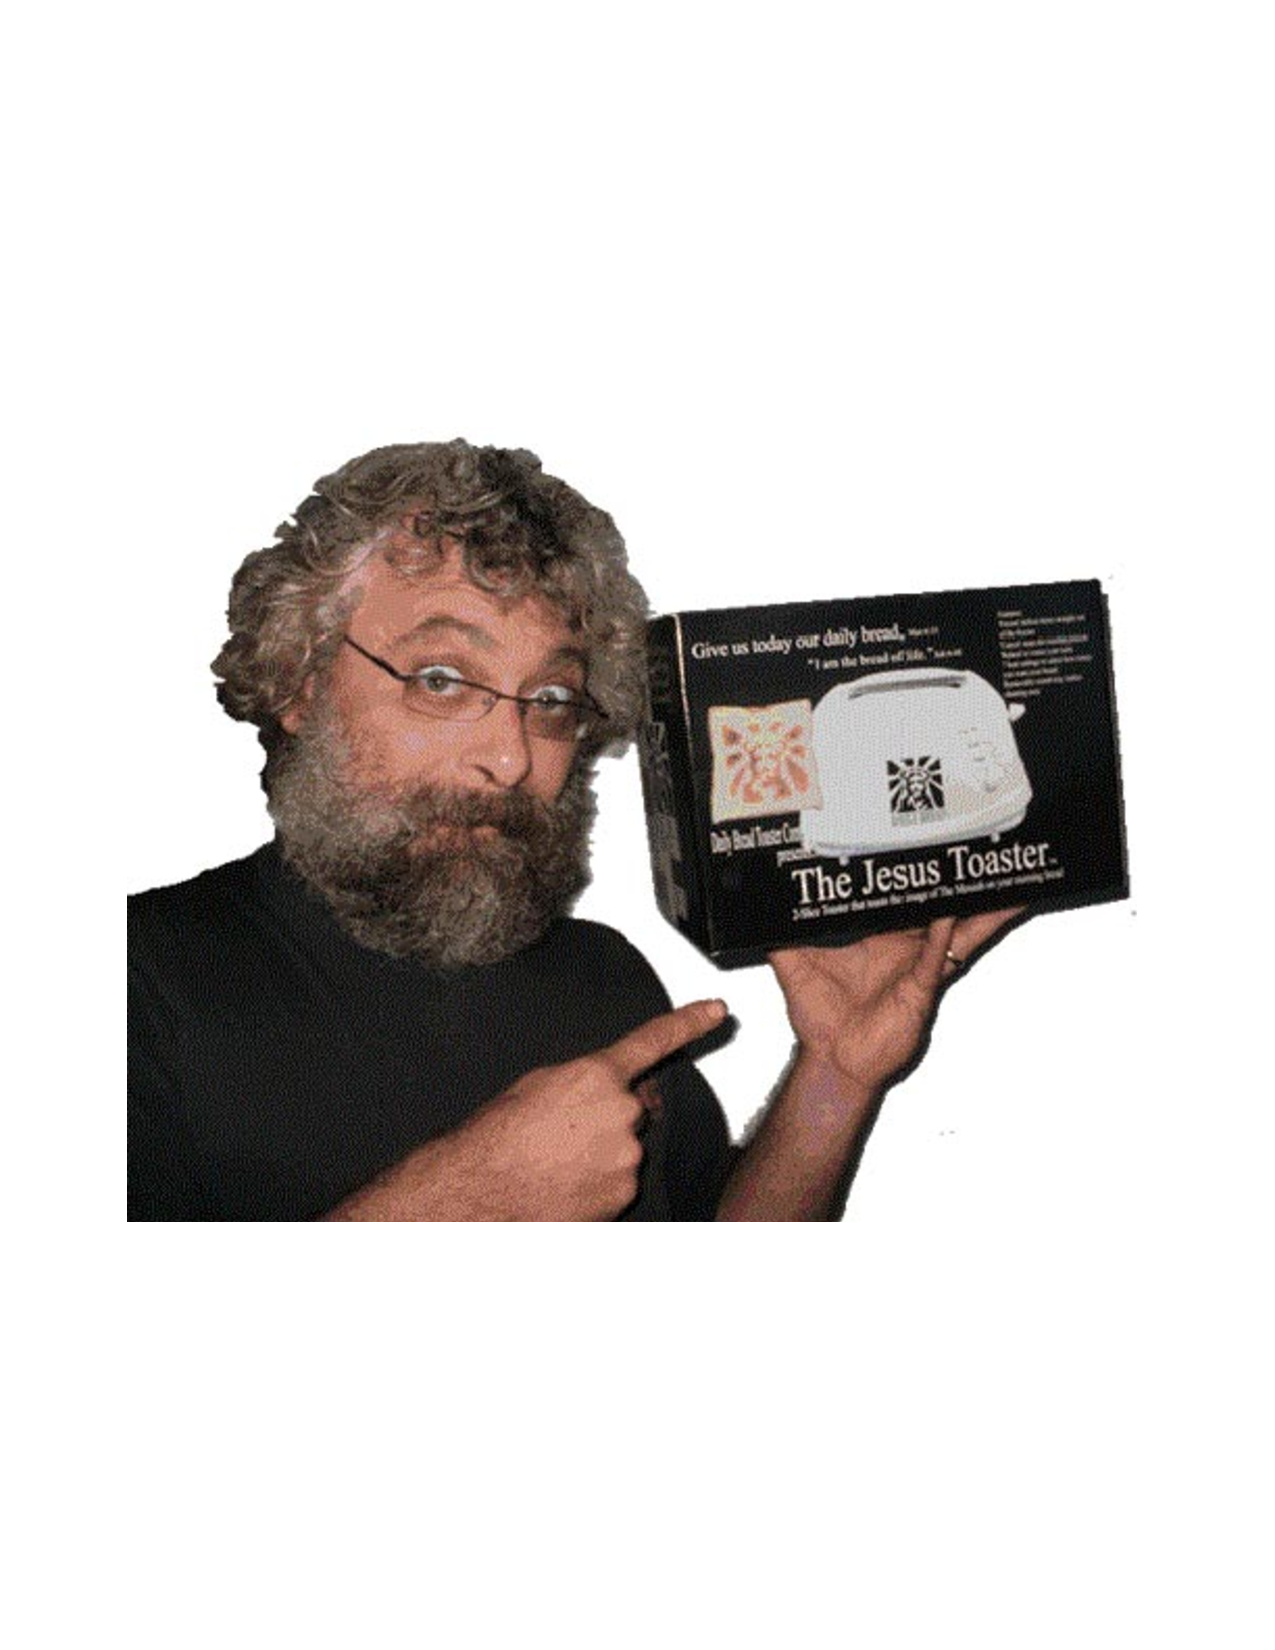
\includegraphics[width=0.39\linewidth]{figures/SM/JesusToaster.pdf}
}
}
\caption{[This figure may not be in the final version] Examples of patterns whose reason for emerging is given by each of the scientifically acceptable explanations. } 
\label{fig:toast}
\end{figure}
Both Figs. \ref{fig:toast} (a) and (b) are examples of patterns arising in systems. The scientifically acceptable explanation for the face seen in Fig. \ref{fig:toast} (a) is the first; namely, that enough pieces of toast are made every year that the appearance of such a face on one piece is a statistically inevitability; you see the face in the toast because a selection bias has arisen: the toast some time ago caught the attention of the media, who delivered it to the public consciousness. The pattern seen in Fig. \ref{fig:toast} (b) is justified by the second scientifically acceptable explanation, namely that some mechanism exists, namely, the mechanism featured in Fig. \ref{fig:toast} (c), to bring about the observed pattern.

\begin{figure}[h]
\makebox[\textwidth][c]{
\centering
\subfloat[]{
  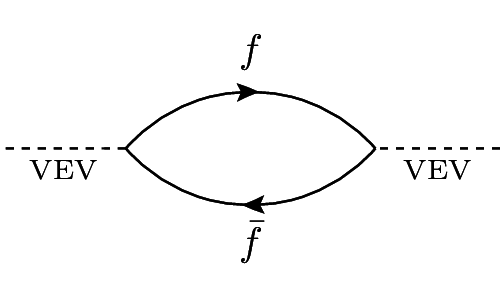
\includegraphics[width=0.5\linewidth]{figures/SM/VevFermionLoop.png}
}
\subfloat[]{
  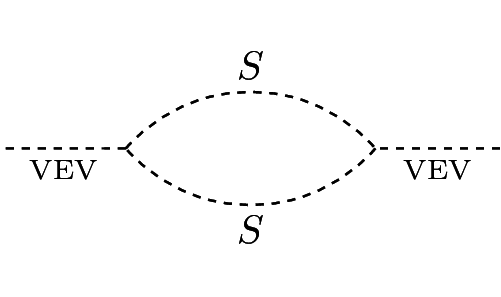
\includegraphics[width=0.5\linewidth]{figures/SM/VevScalarLoop.png}
}
}
\caption{Diagrams for the one-loop corrections to the VEV from a generic fermion (a) and a generic scalar (b).} 
\label{fig:VevLoops}
\end{figure}
The standard model has a number of examples of unexplained fine tuning. Notably, it features a pattern of masses that is quite unusual. As discussed, the origin of particle mass originates from the VEV acquiring a non-zero value through spontaneous symmetry breaking. However, although the VEV is measured to be greater than 200 GeV, it is astonishingly small compared with the natural expectation, and the reason is the following.  The VEV, while normally viewed as a constant in the Lagrangian, actually carries the quantum numbers of the Higgs scalar field, and so interacts with all massive particles. These interactions lead to Feynman diagrams that contain internal loops of the particles. Such diagrams, as in Fig. \ref{fig:VevLoops}, lead to corrections to the value of the VEV given by
\begin{align}
{\rm fermion\hspace{-.1cm}:\ \ }(\Delta {\rm VEV})^2 =& -\frac{\lambda_f^2}{8\pi^2}\cutoff^{2},\label{eq:FermLoop}\\
{\rm scalar\hspace{-.1cm}:\ \ }(\Delta {\rm VEV})^2 =& \hphantom{-} \frac{\lambda_{S}^2}{16\pi^2}[\cutoff^{2}-2m_{S}^2{\rm ln}(\cutoff / m_s)],
\label{eq:ScalarLoop}
\end{align}
where $\lambda_f$ and $\lambda_S$ are the Yukawa coupling and scalar coupling constants, and $\cutoff$ is the cutoff energy of the ultraviolet theory. Every massive particle in the standard model, and in principle any other particle that may occupy the electroweak vacuum, contributes such a correction term. Because $\cutoff$ is near the Planck scale, the VEV receives large corrections that are to $10^{15}$ times larger than the VEV itself. This series of huge numbers is somehow summing to a small number, in a striking example of fine tuning. There is not as yet a scientifically acceptable explanation, since there is no identified mechanism, and no copies of the standard model have been found.

The unexplained cancelation of the 1-loop contributions to the VEV is known as the hierarchy problem, and it impacts nearly every aspect of the standard model. Were the VEV to assume a natural value, the entirety of the particle spectrum of the standard model would be pushed up to the GUT scale. This mystery is especially relevant in the era of TeV-scale particle colliders like the LHC, because a mechanism that could explain the pattern of cancelations is expected to emerge at the electroweak energy scale.  If there is no such mechanism, then we are all but forced to accept the premise that there somehow exists a multitude of versions of the standard model ``somewhere'' in order to make the emergence of such a pattern statistical inevitable. But even in such a case, it is not clear where these copies are, or what selection bias might be responsible for our observing the pattern that is seen. 

\section{Problems with the standard model}
\label{sec:problems}
As stated earlier, there are three reasons why the standard model is believed not to provide a full explanation of all natural phenomena. The first pertains to certain observations that seem to directly contradict predictions of the standard model. The second is the behavior seen in some systems that, while not directly contradicting the predictions of the standard model, seem to go beyond the standard model's ability to account for them. And finally, there is the puzzling observation that the standard model contains a high degree of fine tuning.  While the second issue is of much importance, it is not directly relevant to this work, and so further discussion is left to the literature. However, the following is a discussion of the first and last issue.

\subsection{Observations in tension with the standard model}
The most striking shortcoming of the standard model is that it lacks a description for gravity.  Gravity was the first force to be fully understood over large distances, but it will likely be the last to be fully understood at very short distances. This is because the force of gravity is very weak, as it carries a coupling constant that is $10^{34}$ times smaller than the electromagnetic coupling $\alpha$. Gravitational effects would not be observable in particle collisions below a center of mass energy close to the Planck scale ($10^{19}$ GeV), mindbendingly larger than the energetic reach of modern particle colliders. Most theoretical models that could describe the standard model and gravity, sometimes called theories of everything or ultraviolet (UV) completion models, manifest new phenomena only above a large energy called $\cutoff$, roughly in the vicinity of the Planck scale. 

Another observation not predicted by the standard model is that of neutrino mass.  The Higgs field does not interact with neutrinos because neutrinos are left-chiral and have no right-chiral counterparts (see Figure \ref{tab:SM}); neutrinos in the standard model are massless. However, neutrinos were recently observed to oscillate between flavors \cite{Fukuda:1998mi}, a behavior that is only possible if the neutrinos have mass. This seemingly innocuous observation is in fact quite profound, because it implies that some still unknown theory of particles, with masses of higher energy than the standard model, exists. A number of theories have emerged that could potentially explain neutrino mass, including the types I, II, and III seesaw mechanisms \cite{Yanagida:1980xy}, all of which predict heavy right-handed neutrinos whose mass is inversely proportional to the corresponding left-handed neutrino mass. If a lower bound on the masses of the standard model neutrinos were to be measured, this would specify the mass scale of the heavy neutrinos. Unfortunately, no lower bound has been established as yet, and so there are few clues about the nature of the true theory, or at what energy scale the phenomena of the new theory might be observable.

Another piece of evidence that suggests the standard model falls short of providing a full description of nature is the observation of dark matter in galaxies and in the intergalactic regions of the universe \cite{Davis:1985rj}\cite{Komatsu:2008hk}. Measurements of the baryonic mass of galaxies (the mass due to standard model particles) based on observed galactic luminosities are inconsistent with estimates of the total mass of galaxies based on rates of galactic rotation. The baryonic mass is, on average, a factor 6 lower than the total inferred mass, so it seems that there is a great deal of extra mass in galaxies not accounted for by the known particles.  
\begin{figure}[h]
\makebox[\textwidth][c]{
\centering
\subfloat[]{
  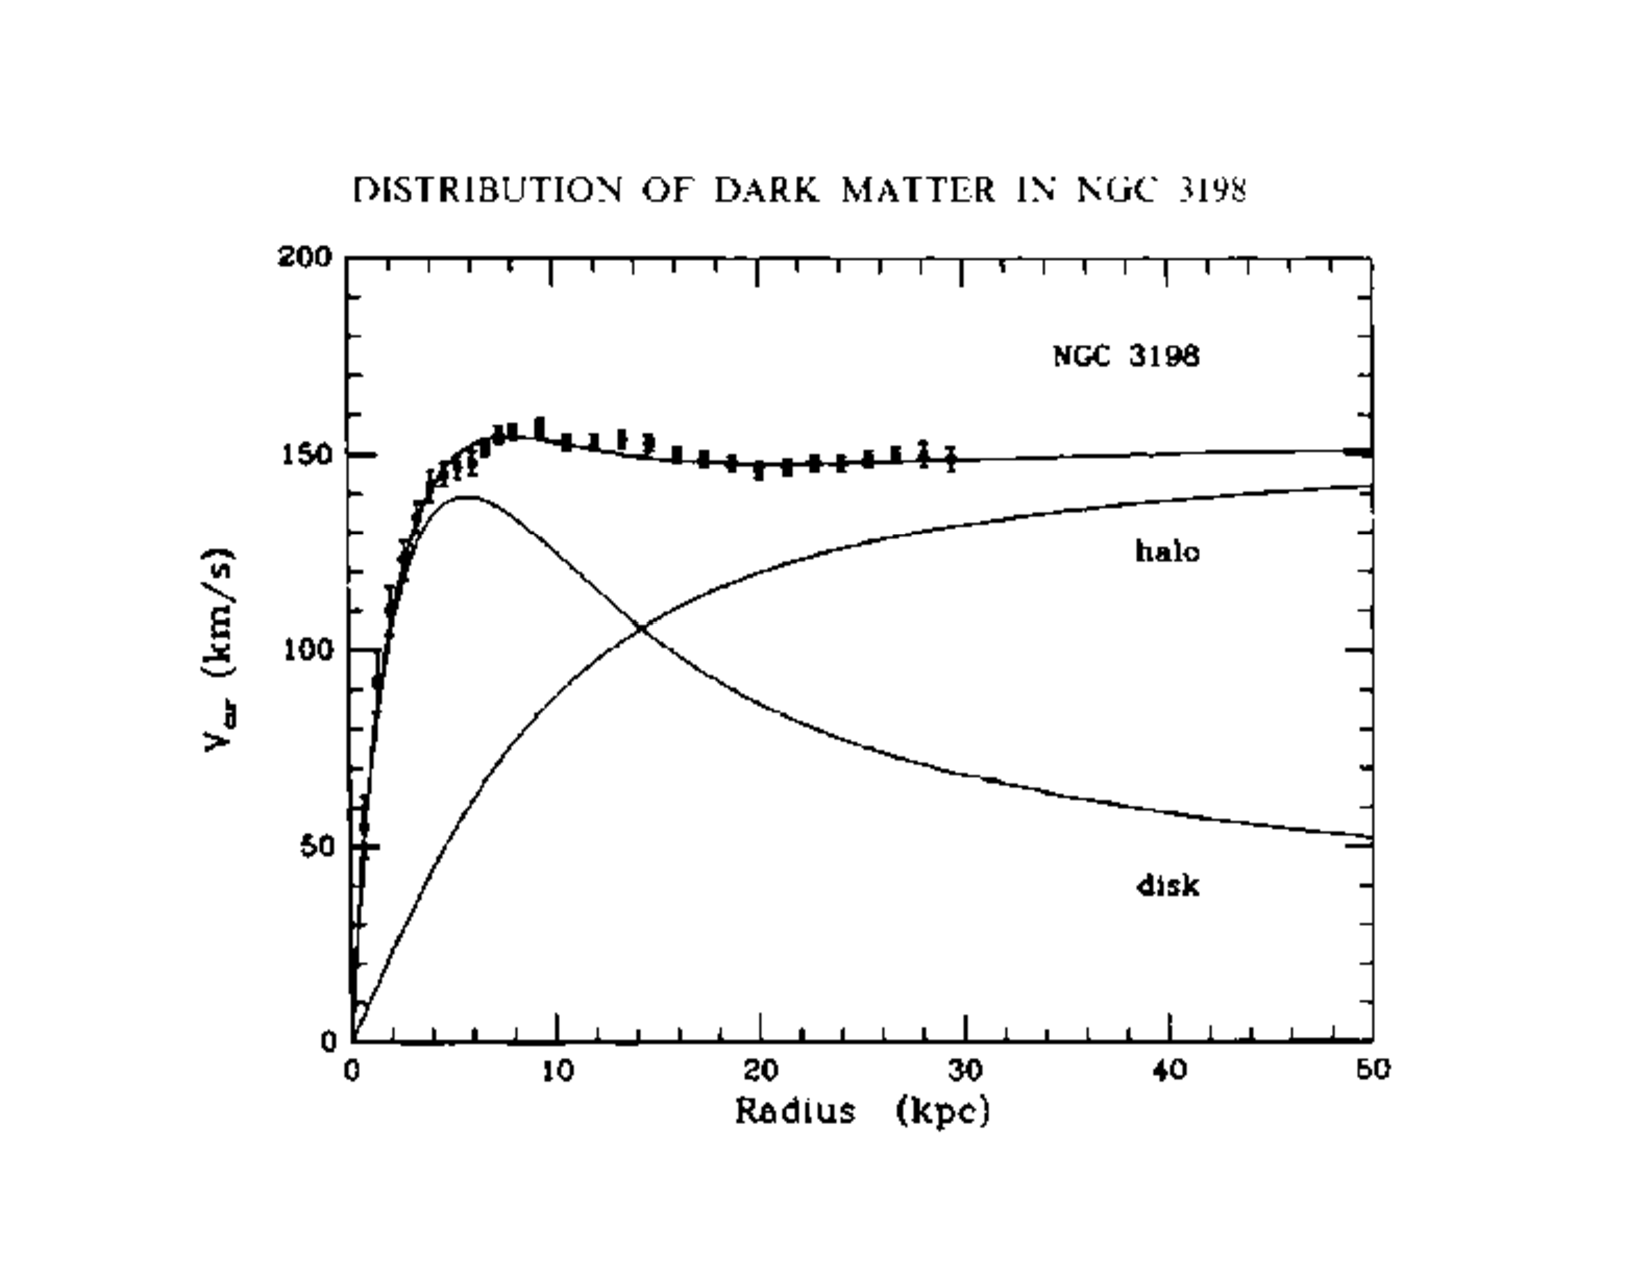
\includegraphics[width=0.6\linewidth]{figures/SM/NGC3198.pdf}
}
\hspace{-.2cm}
\subfloat[]{
  \vspace{2cm}
  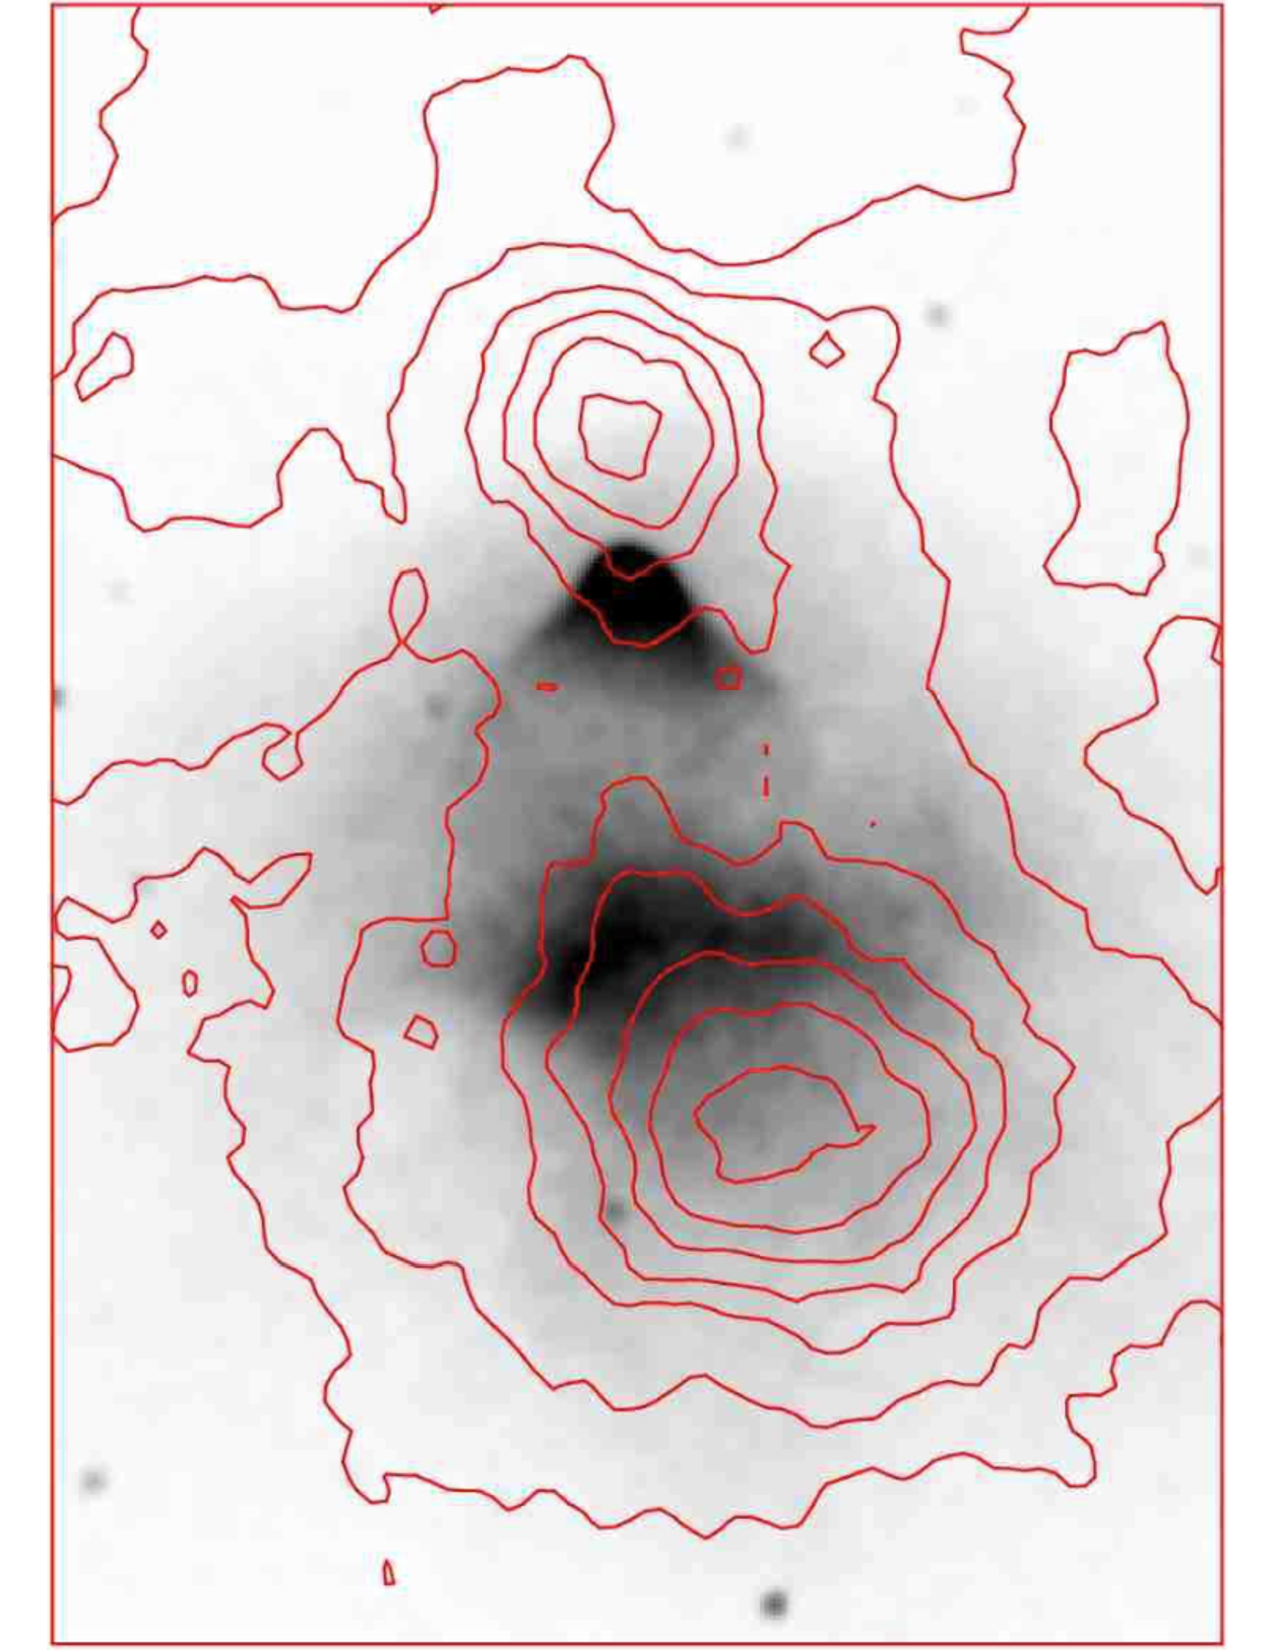
\includegraphics[width=0.46\linewidth]{figures/SM/DMConts.pdf}
}
}
\caption{Subfigure (a) \cite{vanAlbada:1984js} shows the orbital velocity of objects in galaxy NGC 3198 vs their distance from the galactic center. Subfigure (b) \cite{Clowe:2006xq} shows an X-ray photograph taken by the Chandra X-ray observatory of the aftermath of the collision of two galaxy clusters, 1E0657-558, overlaid on a contour map of the gravitation lensing magnitude factor $\kappa$ derived from a separate image taken by the Magellan 6.5 m telescope. } 
\label{fig:DM}
\end{figure}
The best-motivated explanation for this perceived excess is that some yet-undiscovered type of matter exists in abundance within galaxies, but doesn't emit or absorb light (and hence the moniker, ``dark matter''), and therefore has, at most, weak interactions. 

This inferred dark matter may come in the form of new particles, particles not described by the standard model, which may interact with the standard model particles at very high energy scales. This hypothesis is supported by observations of the speed of objects in galaxies as a function of their distance from the galactic center (see Fig. \ref{fig:DM} a). 
The expected speed of objects moving in the nearby galaxy NGC 3198 is given as a function of the orbital radius for the baryonic matter-only hypothesis (solid line peaking at 5 kpc), as well as for the  the baryonic matter+dark matter hypothesis (top solid line). The data (black points) show excellent agreement with the non-interacting dark matter hypothesis. Furthermore, it is claimed that direct evidence of dark matter is evident in the overlay in Figure \ref{fig:DM} (b), in which the aftermath of the collision of two galaxy clusters has been observed. The points of maximum baryonic matter density, represented in black, are displaced from the points of maximum total mass density as determined by the magnitude of gravitational lensing, indicated by the red contours. The interpretation is that the collision of the clusters caused the baryonic matter to collide and slow down, while the dark matter passed through the collision without slowing, resulting in the separation of the two populations of matter.

Dark matter may be discovered by direct or indirect detection experiments (see Ref.~\cite{Undagoitia:2015gya} for a review) or collider experiments like ATLAS \cite{Aad:2008zzm} and CMS \cite{Chatrchyan:2008aa}. A number of theories have been proposed as possible explanations of cosmological dark matter, including certain supersymmetric extensions of the standard model (discussed in Chapter \ref{chap:susy}).


Other observations requiring some explanation beyond the standard model include the fact that there is an abundance of matter in the cosmos but almost no anti-matter (baryon asymmetry), and the existence of the dark energy that accounts for the accelerating expansion of the universe \cite{Goldhaber:2009qu}.

\subsection{Fine tuning and unexplained patterns in the standard model}
\label{sec:finetune}
In a scientific context, tuning is the notion that the parameters of a model can either take on seemingly random values, or they can appear to follow some pattern. An un-tuned (or ``natural'') model refers to the former, and a highly-tuned (or fine-tuned) model refers to the latter. When an apparent pattern has been observed, centuries of science practice and common sense suggests that there should be a reason for the pattern. When a model seems to be fine-tuned, one of two possible, scientifically acceptable explanations must be the case:  
\begin{itemize}
\item{Either there are enough randomized versions (near copies) of the model that the chance emergence of such a pattern is a statistical inevitability; simultaneously, some kind of selection bias has lead the observer to examine the particular instance of the model that exhibited the pattern; or}
\item{there exists some mechanism that generates the observed pattern. }
\end{itemize}

\begin{figure}[h]
\makebox[\textwidth][c]{
\centering
\subfloat[]{
  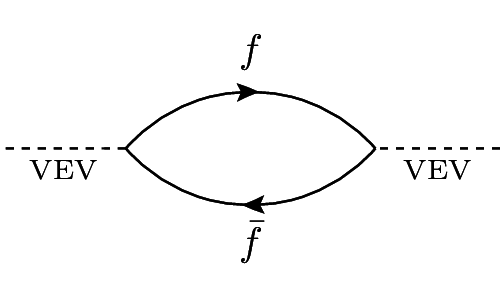
\includegraphics[width=0.5\linewidth]{figures/SM/VevFermionLoop.png}
}
\subfloat[]{
  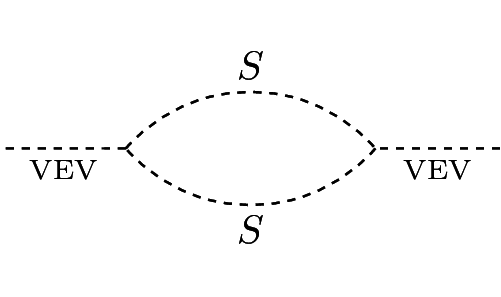
\includegraphics[width=0.5\linewidth]{figures/SM/VevScalarLoop.png}
}
}
\caption{Diagrams for the one-loop corrections to the VEV from a generic fermion (a) and a generic scalar (b).} 
\label{fig:VevLoops}
\end{figure}
The standard model has a number of examples of unexplained fine tuning. Notably, it features a pattern of masses that is quite unusual. As discussed, the origin of particle mass originates from the VEV acquiring a non-zero value through spontaneous symmetry breaking. However, although the VEV is measured to be greater than 200 GeV, it is astonishingly small compared with the natural expectation, and the reason is the following.  The VEV, while normally viewed as a constant in the Lagrangian, actually carries the quantum numbers of the Higgs scalar field, and so interacts with all massive particles. These interactions lead to Feynman diagrams that contain internal loops of the particles. Such diagrams, as in Fig. \ref{fig:VevLoops}, lead to corrections to the value of the VEV given by
\begin{align}
{\rm fermion\hspace{-.1cm}:\ \ }(\Delta {\rm VEV})^2 =& -\frac{\lambda_f^2}{8\pi^2}\cutoff^{2},\label{eq:FermLoop}\\
{\rm scalar\hspace{-.1cm}:\ \ }(\Delta {\rm VEV})^2 =& \hphantom{-} \frac{\lambda_{S}^2}{16\pi^2}[\cutoff^{2}-2m_{S}^2{\rm ln}(\cutoff / m_s)],
\label{eq:ScalarLoop}
\end{align}
where $\lambda_f$ and $\lambda_S$ are the Yukawa coupling and scalar coupling constants, and $\cutoff$ is the cutoff energy of the ultraviolet theory. Every massive particle in the standard model, and in principle any other particle that may occupy the electroweak vacuum, contributes such a correction term. Because $\cutoff$ is near the Planck scale, the VEV receives large corrections that are to $10^{15}$ times larger than the VEV itself. This series of huge numbers is somehow summing to a small number, in a striking example of fine tuning. There is not as yet a scientifically acceptable explanation, since there is no identified mechanism, and no copies of the standard model have been found.

The unexplained cancelation of the 1-loop contributions to the VEV is known as the hierarchy problem, and it impacts nearly every aspect of the standard model. Were the VEV to assume a natural value, the entirety of the particle spectrum of the standard model would be pushed up to the GUT scale. This mystery is especially relevant in the era of TeV-scale particle colliders like the LHC, because a mechanism that could explain the pattern of cancelations is expected to emerge at the electroweak energy scale.  If there is no such mechanism, then we are all but forced to accept the premise that there somehow exists a multitude of versions of the standard model ``somewhere'' in order to make the emergence of such a pattern statistical inevitable. But even in such a case, it is not clear where these copies are, or what selection bias might be responsible for our observing the pattern that is seen. 

\section{Problems with the standard model}
\label{sec:problems}
As stated earlier, there are three reasons why the standard model is believed not to provide a full explanation of all natural phenomena. The first pertains to certain observations that seem to directly contradict predictions of the standard model. The second is the behavior seen in some systems that, while not directly contradicting the predictions of the standard model, seem to go beyond the standard model's ability to account for them. And finally, there is the puzzling observation that the standard model contains a high degree of fine tuning.  While the second issue is of much importance, it is not directly relevant to this work, and so further discussion is left to the literature. However, the following is a discussion of the first and last issue.

\subsection{Observations in tension with the standard model}
The most striking shortcoming of the standard model is that it lacks a description for gravity.  Gravity was the first force to be fully understood over large distances, but it will likely be the last to be fully understood at very short distances. This is because the force of gravity is very weak, as it carries a coupling constant that is $10^{34}$ times smaller than the electromagnetic coupling $\alpha$. Gravitational effects would not be observable in particle collisions below a center of mass energy close to the Planck scale ($10^{19}$ GeV), mindbendingly larger than the energetic reach of modern particle colliders. Most theoretical models that could describe the standard model and gravity, sometimes called theories of everything or ultraviolet (UV) completion models, manifest new phenomena only above a large energy called $\cutoff$, roughly in the vicinity of the Planck scale. 

Another observation not predicted by the standard model is that of neutrino mass.  The Higgs field does not interact with neutrinos because neutrinos are left-chiral and have no right-chiral counterparts (see Figure \ref{tab:SM}); neutrinos in the standard model are massless. However, neutrinos were recently observed to oscillate between flavors \cite{Fukuda:1998mi}, a behavior that is only possible if the neutrinos have mass. This seemingly innocuous observation is in fact quite profound, because it implies that some still unknown theory of particles, with masses of higher energy than the standard model, exists. A number of theories have emerged that could potentially explain neutrino mass, including the types I, II, and III seesaw mechanisms \cite{Yanagida:1980xy}, all of which predict heavy right-handed neutrinos whose mass is inversely proportional to the corresponding left-handed neutrino mass. If a lower bound on the masses of the standard model neutrinos were to be measured, this would specify the mass scale of the heavy neutrinos. Unfortunately, no lower bound has been established as yet, and so there are few clues about the nature of the true theory, or at what energy scale the phenomena of the new theory might be observable.

Another piece of evidence that suggests the standard model falls short of providing a full description of nature is the observation of dark matter in galaxies and in the intergalactic regions of the universe \cite{Davis:1985rj}\cite{Komatsu:2008hk}. Measurements of the baryonic mass of galaxies (the mass due to standard model particles) based on observed galactic luminosities are inconsistent with estimates of the total mass of galaxies based on rates of galactic rotation. The baryonic mass is, on average, a factor 6 lower than the total inferred mass, so it seems that there is a great deal of extra mass in galaxies not accounted for by the known particles.  
\begin{figure}[h]
\makebox[\textwidth][c]{
\centering
\subfloat[]{
  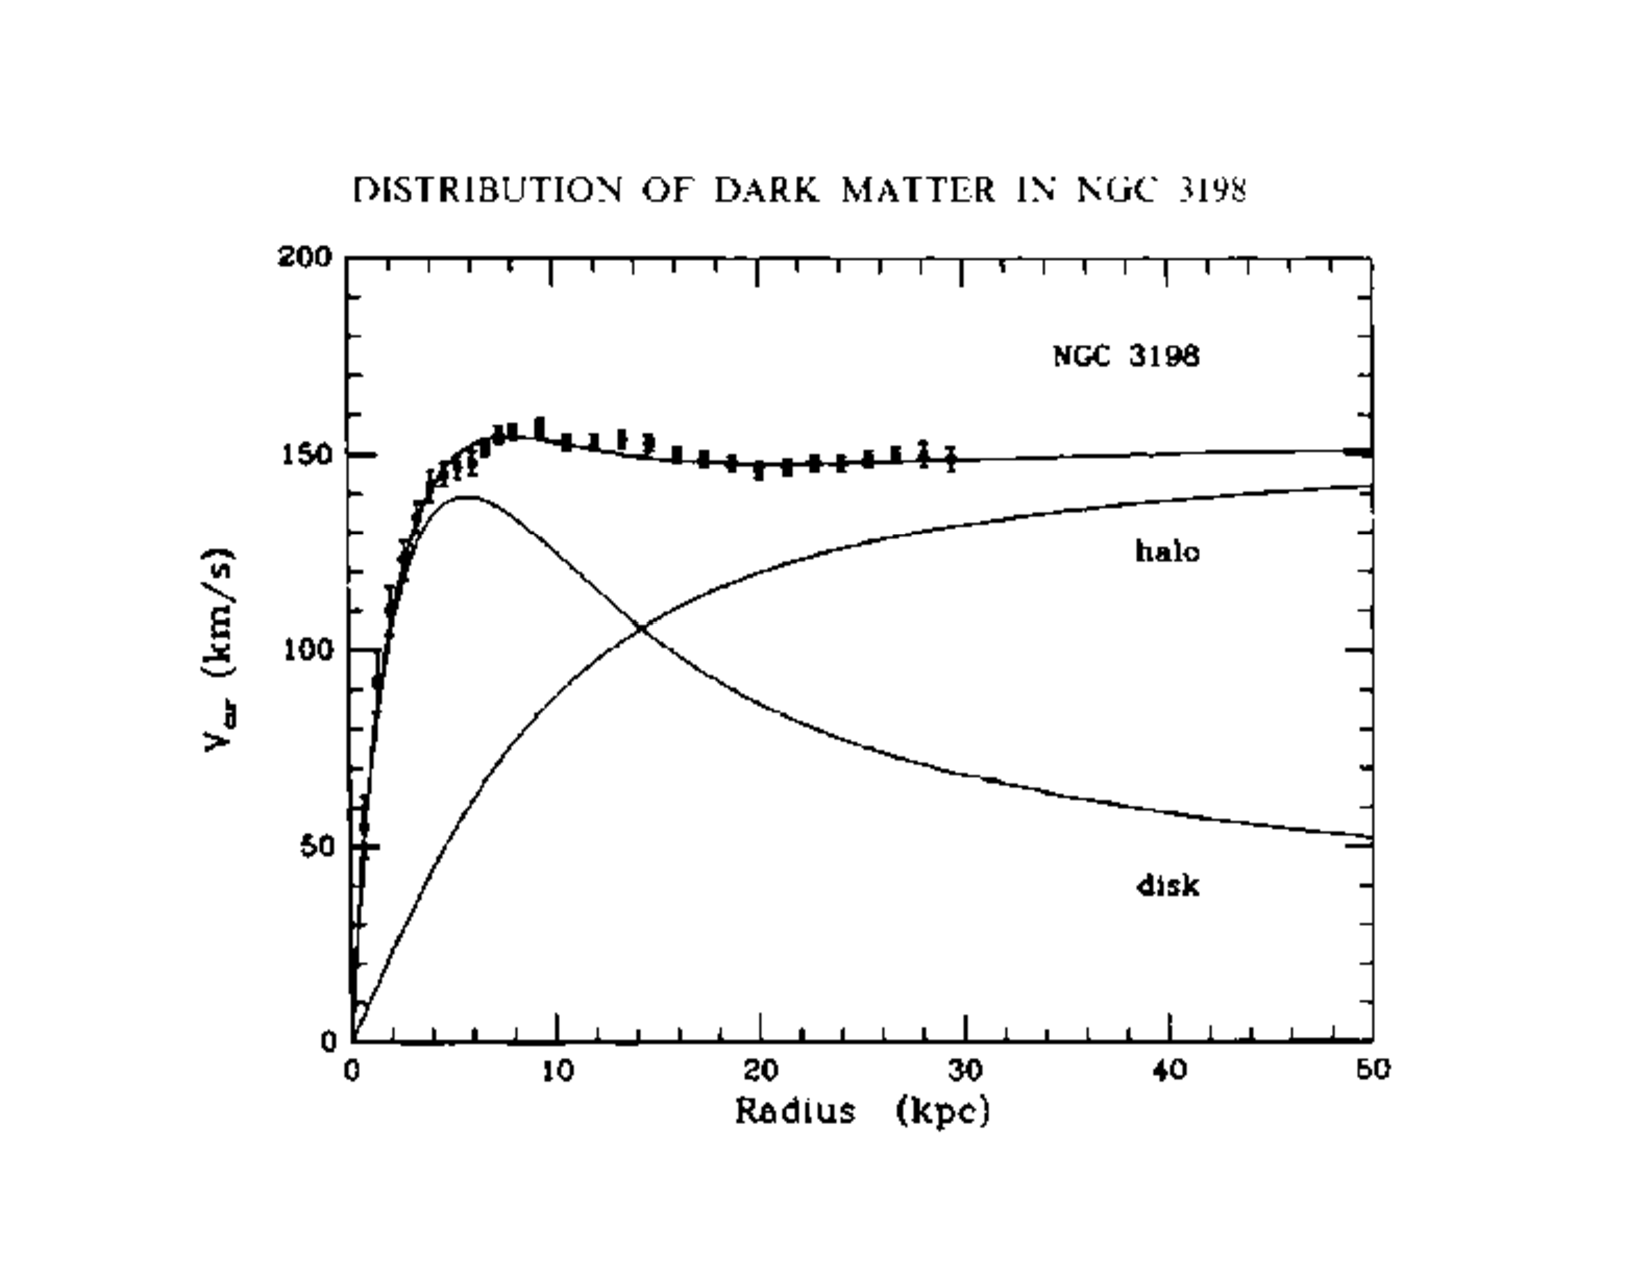
\includegraphics[width=0.6\linewidth]{figures/SM/NGC3198.pdf}
}
\hspace{-.2cm}
\subfloat[]{
  \vspace{2cm}
  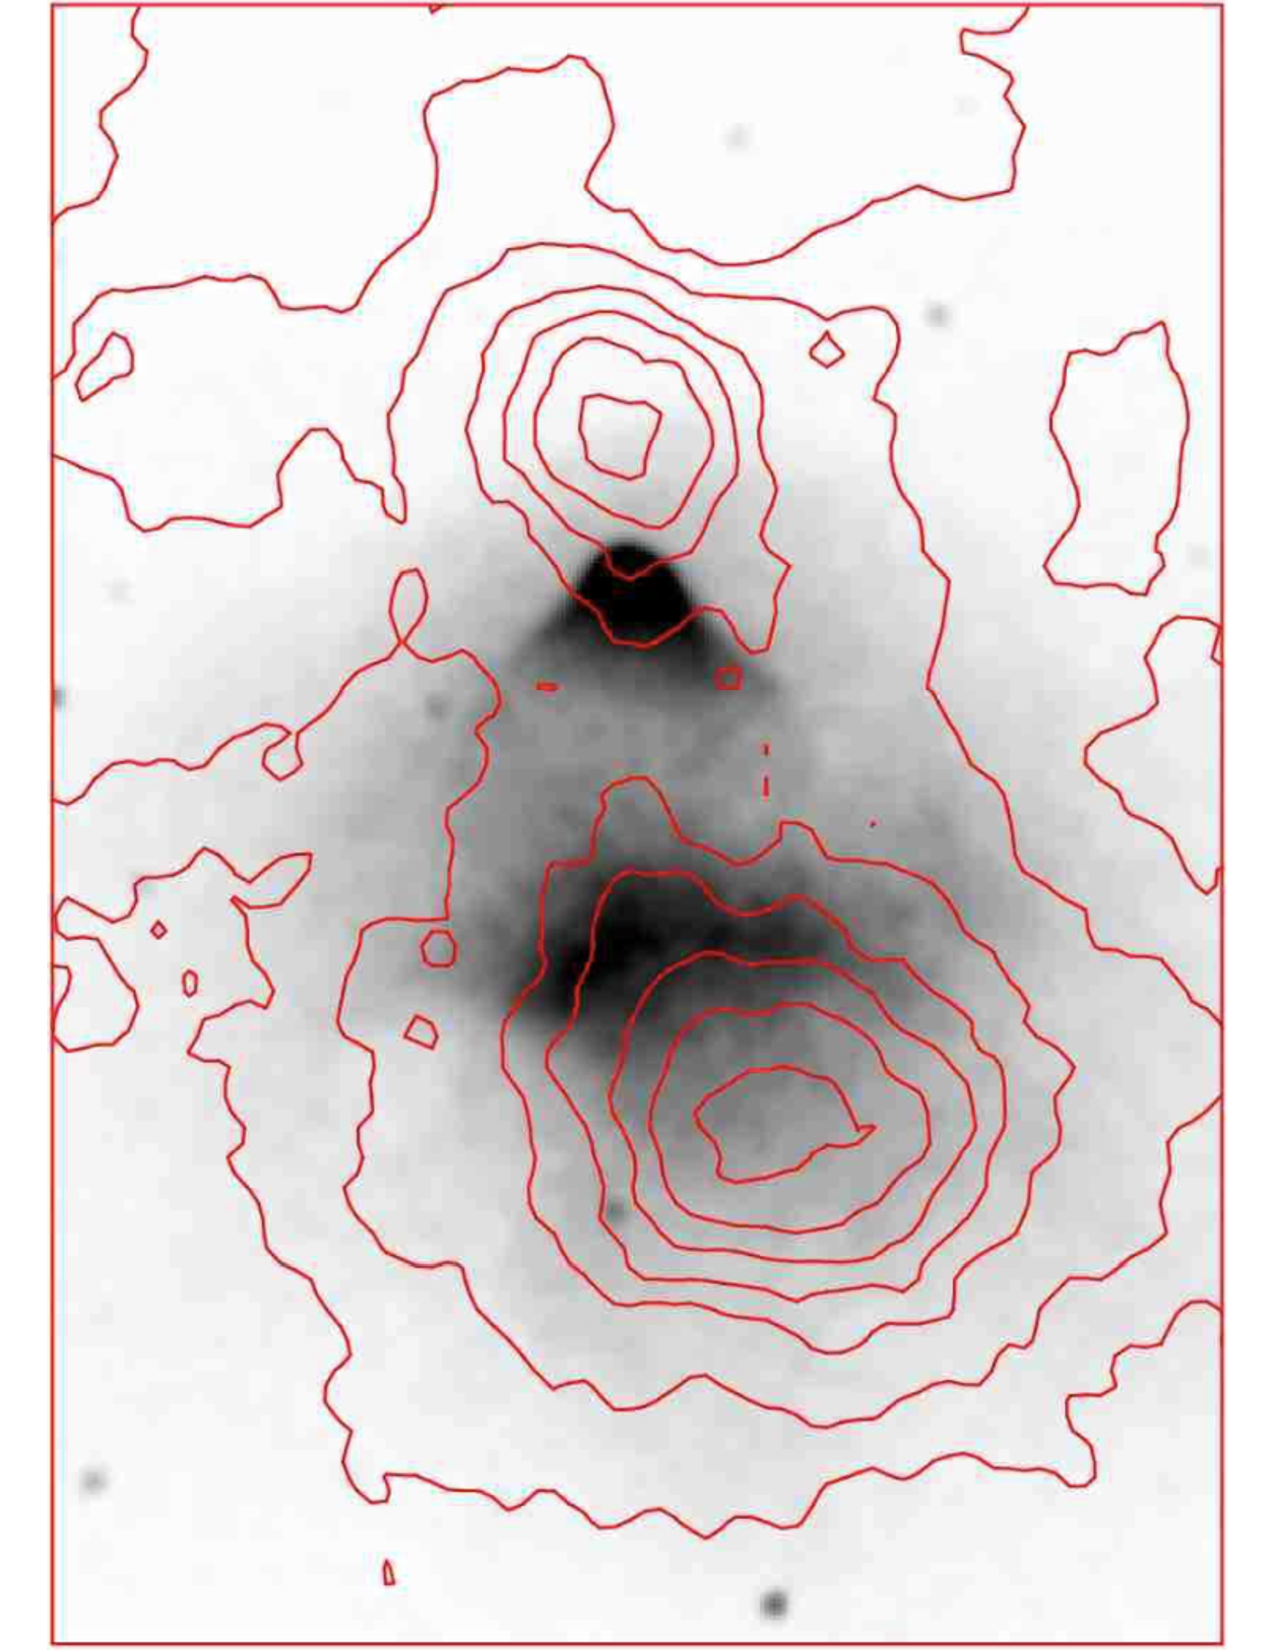
\includegraphics[width=0.46\linewidth]{figures/SM/DMConts.pdf}
}
}
\caption{Subfigure (a) \cite{vanAlbada:1984js} shows the orbital velocity of objects in galaxy NGC 3198 vs their distance from the galactic center. Subfigure (b) \cite{Clowe:2006xq} shows an X-ray photograph taken by the Chandra X-ray observatory of the aftermath of the collision of two galaxy clusters, 1E0657-558, overlaid on a contour map of the gravitation lensing magnitude factor $\kappa$ derived from a separate image taken by the Magellan 6.5 m telescope. } 
\label{fig:DM}
\end{figure}
The best-motivated explanation for this perceived excess is that some yet-undiscovered type of matter exists in abundance within galaxies, but doesn't emit or absorb light (and hence the moniker, ``dark matter''), and therefore has, at most, weak interactions. 

This inferred dark matter may come in the form of new particles, particles not described by the standard model, which may interact with the standard model particles at very high energy scales. This hypothesis is supported by observations of the speed of objects in galaxies as a function of their distance from the galactic center (see Fig. \ref{fig:DM} a). 
The expected speed of objects moving in the nearby galaxy NGC 3198 is given as a function of the orbital radius for the baryonic matter-only hypothesis (solid line peaking at 5 kpc), as well as for the  the baryonic matter+dark matter hypothesis (top solid line). The data (black points) show excellent agreement with the non-interacting dark matter hypothesis. Furthermore, it is claimed that direct evidence of dark matter is evident in the overlay in Figure \ref{fig:DM} (b), in which the aftermath of the collision of two galaxy clusters has been observed. The points of maximum baryonic matter density, represented in black, are displaced from the points of maximum total mass density as determined by the magnitude of gravitational lensing, indicated by the red contours. The interpretation is that the collision of the clusters caused the baryonic matter to collide and slow down, while the dark matter passed through the collision without slowing, resulting in the separation of the two populations of matter.

Dark matter may be discovered by direct or indirect detection experiments (see Ref.~\cite{Undagoitia:2015gya} for a review) or collider experiments like ATLAS \cite{Aad:2008zzm} and CMS \cite{Chatrchyan:2008aa}. A number of theories have been proposed as possible explanations of cosmological dark matter, including certain supersymmetric extensions of the standard model (discussed in Chapter \ref{chap:susy}).


Other observations requiring some explanation beyond the standard model include the fact that there is an abundance of matter in the cosmos but almost no anti-matter (baryon asymmetry), and the existence of the dark energy that accounts for the accelerating expansion of the universe \cite{Goldhaber:2009qu}.

\subsection{Fine tuning and unexplained patterns in the standard model}
\label{sec:finetune}
In a scientific context, tuning is the notion that the parameters of a model can either take on seemingly random values, or they can appear to follow some pattern. An un-tuned (or ``natural'') model refers to the former, and a highly-tuned (or fine-tuned) model refers to the latter. When an apparent pattern has been observed, centuries of science practice and common sense suggests that there should be a reason for the pattern. When a model seems to be fine-tuned, one of two possible, scientifically acceptable explanations must be the case:  
\begin{itemize}
\item{Either there are enough randomized versions (near copies) of the model that the chance emergence of such a pattern is a statistical inevitability; simultaneously, some kind of selection bias has lead the observer to examine the particular instance of the model that exhibited the pattern; or}
\item{there exists some mechanism that generates the observed pattern. }
\end{itemize}
For example, suppose you are shown a piece of toast with the pattern of a religious figure on the face, as in Figure \ref{fig:toast} (a) or (b). 
\begin{figure}[h]
\makebox[\textwidth][c]{
\centering
\subfloat[]{
  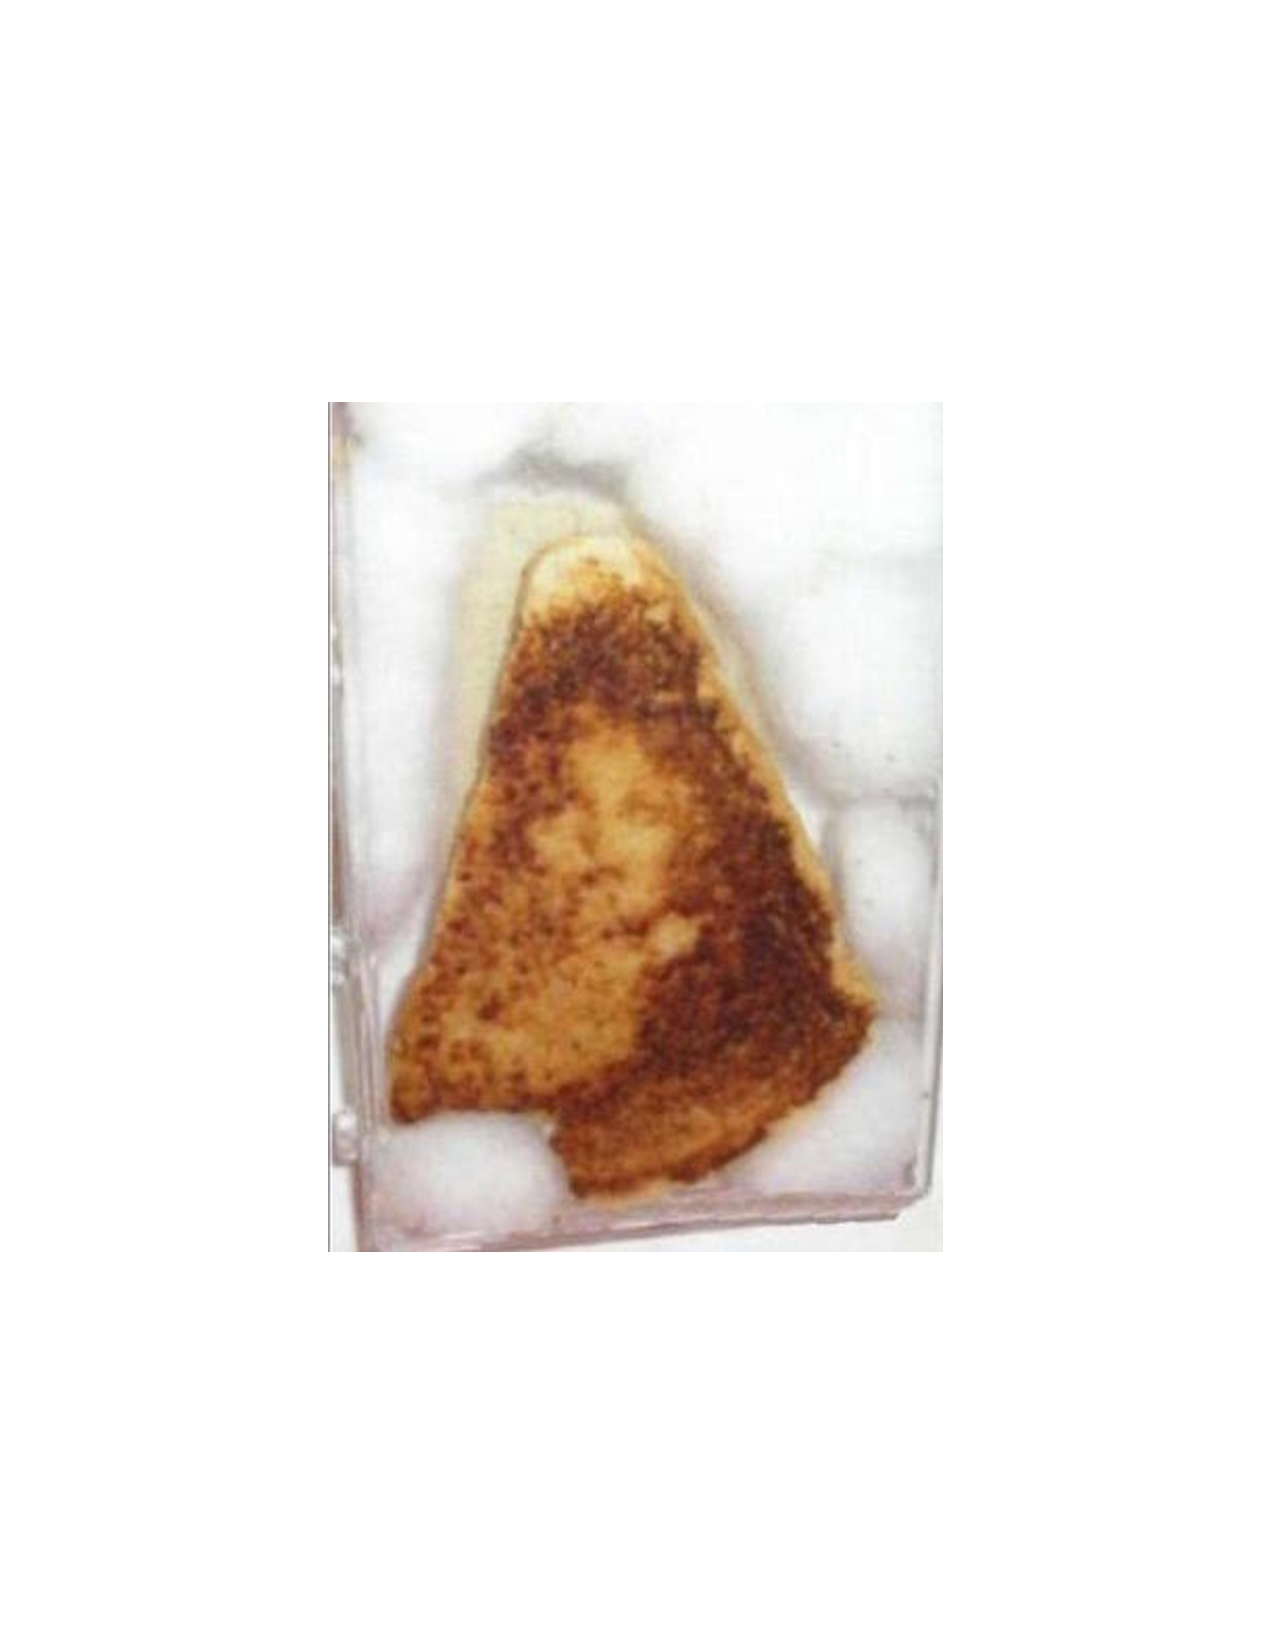
\includegraphics[width=0.3\linewidth]{figures/SM/Mary.pdf}
}
\hspace{-.2cm}
\subfloat[]{
  \vspace{2cm}
  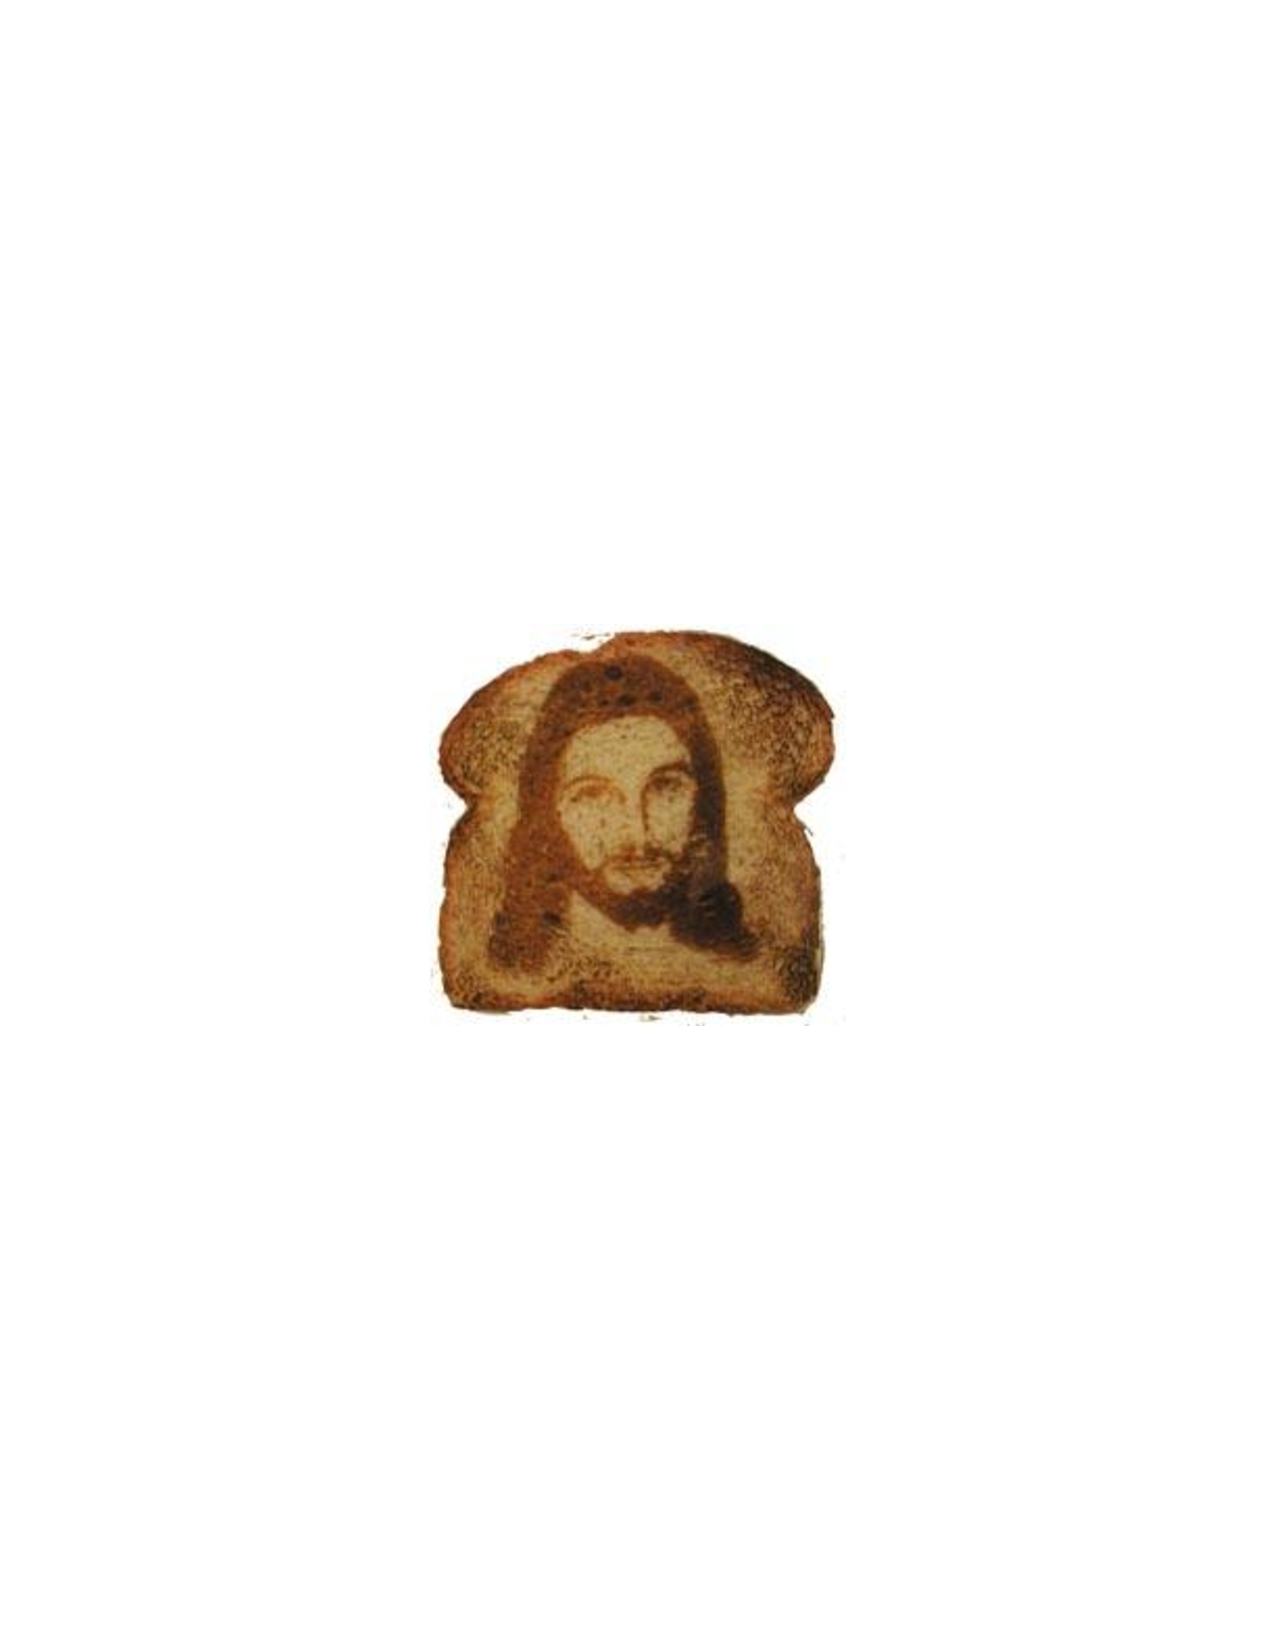
\includegraphics[width=0.33\linewidth]{figures/SM/Jesus.pdf}
}
\hspace{-.2cm}
\subfloat[]{
  \vspace{2cm}
  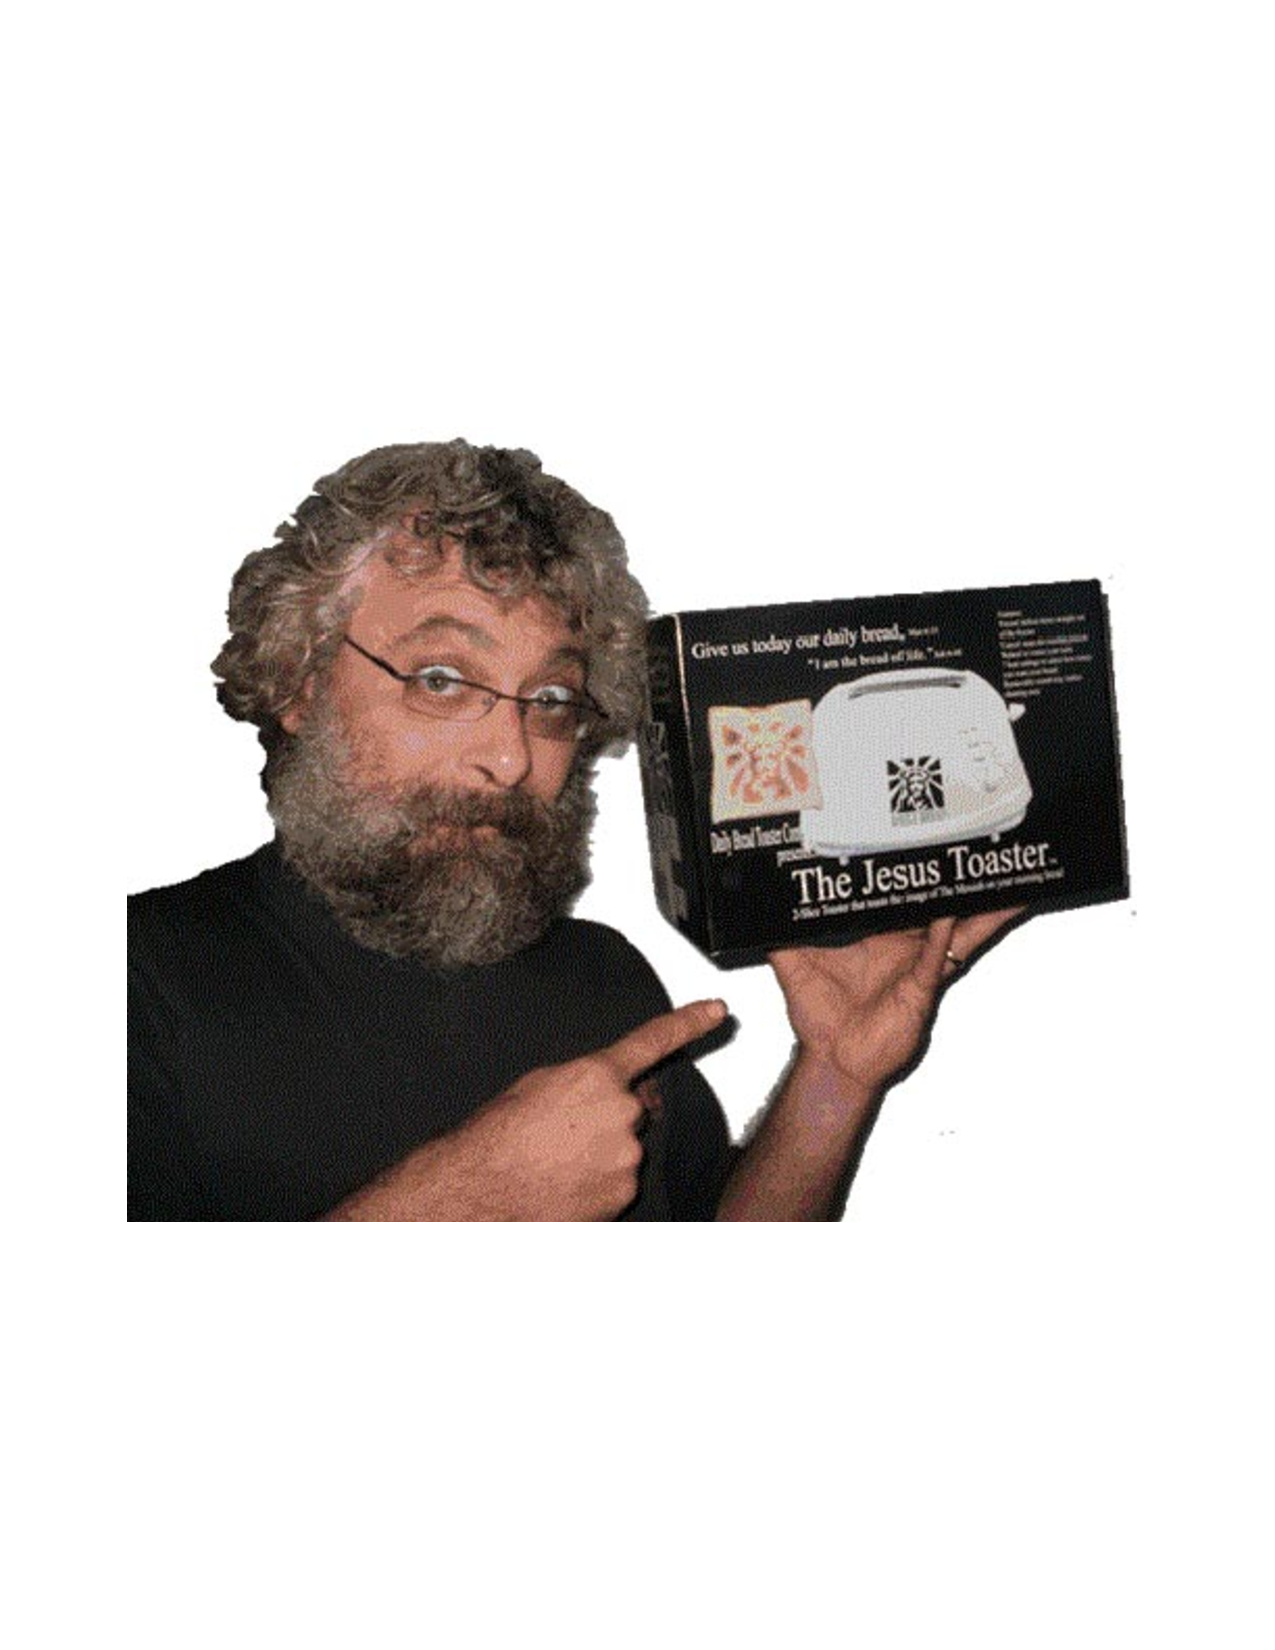
\includegraphics[width=0.39\linewidth]{figures/SM/JesusToaster.pdf}
}
}
\caption{[This figure may not be in the final version] Examples of patterns whose reason for emerging is given by each of the scientifically acceptable explanations. } 
\label{fig:toast}
\end{figure}
Both Figs. \ref{fig:toast} (a) and (b) are examples of patterns arising in systems. The scientifically acceptable explanation for the face seen in Fig. \ref{fig:toast} (a) is the first; namely, that enough pieces of toast are made every year that the appearance of such a face on one piece is a statistically inevitability; you see the face in the toast because a selection bias has arisen: the toast some time ago caught the attention of the media, who delivered it to the public consciousness. The pattern seen in Fig. \ref{fig:toast} (b) is justified by the second scientifically acceptable explanation, namely that some mechanism exists, namely, the mechanism featured in Fig. \ref{fig:toast} (c), to bring about the observed pattern.

\begin{figure}[h]
\makebox[\textwidth][c]{
\centering
\subfloat[]{
  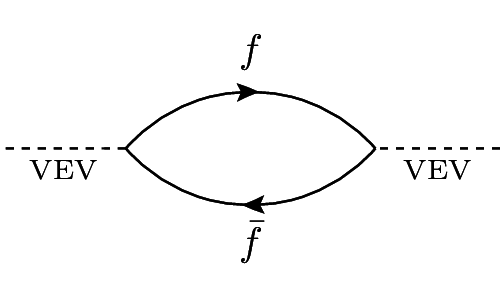
\includegraphics[width=0.5\linewidth]{figures/SM/VevFermionLoop.png}
}
\subfloat[]{
  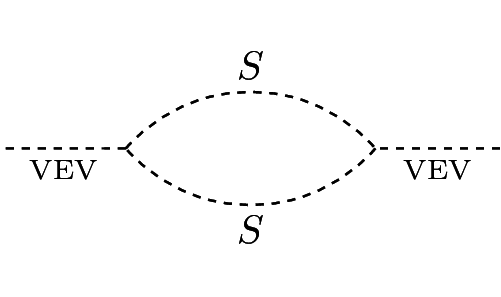
\includegraphics[width=0.5\linewidth]{figures/SM/VevScalarLoop.png}
}
}
\caption{Diagrams for the one-loop corrections to the VEV from a generic fermion (a) and a generic scalar (b).} 
\label{fig:VevLoops}
\end{figure}
The standard model has a number of examples of unexplained fine tuning. Notably, it features a pattern of masses that is quite unusual. As discussed, the origin of particle mass originates from the VEV acquiring a non-zero value through spontaneous symmetry breaking. However, although the VEV is measured to be greater than 200 GeV, it is astonishingly small compared with the natural expectation, and the reason is the following.  The VEV, while normally viewed as a constant in the Lagrangian, actually carries the quantum numbers of the Higgs scalar field, and so interacts with all massive particles. These interactions lead to Feynman diagrams that contain internal loops of the particles. Such diagrams, as in Fig. \ref{fig:VevLoops}, lead to corrections to the value of the VEV given by
\begin{align}
{\rm fermion\hspace{-.1cm}:\ \ }(\Delta {\rm VEV})^2 =& -\frac{\lambda_f^2}{8\pi^2}\cutoff^{2},\label{eq:FermLoop}\\
{\rm scalar\hspace{-.1cm}:\ \ }(\Delta {\rm VEV})^2 =& \hphantom{-} \frac{\lambda_{S}^2}{16\pi^2}[\cutoff^{2}-2m_{S}^2{\rm ln}(\cutoff / m_s)],
\label{eq:ScalarLoop}
\end{align}
where $\lambda_f$ and $\lambda_S$ are the Yukawa coupling and scalar coupling constants, and $\cutoff$ is the cutoff energy of the ultraviolet theory. Every massive particle in the standard model, and in principle any other particle that may occupy the electroweak vacuum, contributes such a correction term. Because $\cutoff$ is near the Planck scale, the VEV receives large corrections that are to $10^{15}$ times larger than the VEV itself. This series of huge numbers is somehow summing to a small number, in a striking example of fine tuning. There is not as yet a scientifically acceptable explanation, since there is no identified mechanism, and no copies of the standard model have been found.

The unexplained cancelation of the 1-loop contributions to the VEV is known as the hierarchy problem, and it impacts nearly every aspect of the standard model. Were the VEV to assume a natural value, the entirety of the particle spectrum of the standard model would be pushed up to the GUT scale. This mystery is especially relevant in the era of TeV-scale particle colliders like the LHC, because a mechanism that could explain the pattern of cancelations is expected to emerge at the electroweak energy scale.  If there is no such mechanism, then we are all but forced to accept the premise that there somehow exists a multitude of versions of the standard model ``somewhere'' in order to make the emergence of such a pattern statistical inevitable. But even in such a case, it is not clear where these copies are, or what selection bias might be responsible for our observing the pattern that is seen. 

\section{This document}

The subject of this dissertation is a symmetry, that, if realized in the context of the $\sm$, may resolve a number of the above mentioned riddles, including the hierarchy problem. The symmetry, known as $\SUSY$ \cite{Martin:1997ns}, is the only remaining spacetime symmetry not yet found in nature. Supersymmetry offers a potentially viable explanation for the existence of dark matter, and if ever discovered, could motivate certain models of grand unification, theories of everything, and string theories. 

This document summarizes work that has been carried out to shed light on the question of whether a supersymmetric extension of the $\sm$ is possible given the observations made so far by the Compact Muon Solenoid (CMS), and if not, whether a definitive answer can be expected from analysis of current and future experimental data. Additionally, analysis techniques are discussed that have been applied to the Run 2 (2015) dataset. I have authored the text in a style suitable for a graduate student interested in contributing to the effort of globally understanding the experimental viability of supersymmetry, and in developing new techniques to search for  supersymmetry at the Large Hadron Collider (LHC).

The body of this document is organized as follows. I proceed with a brief description of supersymmetry and how it may manifest itself at the LHC.  Chapter \ref{chap:lhc} gives a description of the LHC, and Chapter \ref{chap:cms} provides a description the Compact Muon Solenoid (CMS). During the discussion of the CMS detector, I make short forays into studies and techniques I have developed while contributing to a number of technical upgrades within CMS. 

In Chapter \ref{chap:run1pmssm}, I describe an analysis~\cite{Khachatryan:2016nvf} I helped perform within CMS to understand how the hypothesis of supersymmtry is constrained by the data that has been collected and analyzed by CMS and other experiments. The analysis is a global interpretation of a representative set of CMS SUSY searches in the context of a general model of supersymmetry that is a proxy for the 120-parameter model called the minimal supersymmetric standard model. The submodel is called the phenomenological MSSM (pMSSM). The goal of the chapter is to summarize what lessons have been learned about the viability of supersymmetric hypotheses based on LHC results. 

In Chapter \ref{chap:susysearches}, I proceed to describe various analysis techniques that I have developed to improve the sensitivity of CMS searches to supersymmetry models that have not been excluded by the CMS Run 1 (2011-2012) analyses. This includes novel methods for modeling of Standard Model QCD and $\zinv$ processes, which are dominant sources of background in searches that look for evidence of supersymmetry, as well as novel techniques for modeling triggers (triggers are defined in Chapter \ref{chap:cms}) useful for analyses that are brave enough to hunt for supersymmetry in kinematic regions where the background is dominant. I also give key details about two 2015 and 2016 analyses that I contributed to while developing the mentioned techniques \cite{Khachatryan:2016kdk}\cite{CMS:2016nhb}. The chapter ends with a proof of principal demonstration of a bold strategy for searching for evidence of supersymmetry, namely, the feasibility of employing multivariate discriminants to maximize sensitivity to models of supersymmetry.

Chapter \ref{chap:ma5} summarizes contributions I made to a project~\cite{Dumont:2014tja} outside the CMS collaboration that has the goal of making the results of CMS and ATLAS SUSY searches more accessible to the theoretical physics community. 

\chapter{Supersymmetry}
\label{chap:susy}
Supersymmetry was originally developed out of an attempt to understand why all particle interactions seem to obey Poincar{\'e} symmetries, but not all interactions allowed by the Poincar{\'e} group are are manifest in nature \cite{Golfand:1971iw, Wess:1974tw}. The idea that a larger symmetry may exist, one that governs which interactions are allowed and which are not, was a prevailing source of curiosity at the time, and remains so today. 

Because the ten generators of the Poincar{\'e} group have been mapped to the non-spin related spacetime symmetries (four translations, three rotations, and three boosts), it is natural to suppose that any larger symmetry containing the Poincar{\'e} group should involve the only remaining degrees of freedom, namely spin. Such a symmetry, which is called a supersymmetry, would generate transformations that shift quantum states by a fundamental unit of spin, $\hbar$/2, modeled as the action of an operator $\hat{Q}$ such that
\begin{equation}
\label{eq:SusyOperators}
\hat{Q}\ket{\text{boson}}=\ket{\text{fermion}},\text{\ \ \ } \hat{Q}\ket{\text{fermion}}=\ket{\text{boson}}.
\end{equation}
Since the $\ket{\text{boson}}$ and $\ket{\text{fermion}}$ states differ by a spin of $\hbar$/2, conservation of angular momentum requires that the operator $\hat{Q}$ itself carry spin $\hbar$/2, and so $\hat{Q}$ is identified as a fermionic operator obeying the fermion anti-commutation relations
\begin{equation}
\acomm{\hat{Q}_\alpha}{\hat{Q}_{\dot{\beta}}^\dag}=-2\sigma^{\mu}_{\alpha \dot{\beta}}\hat{P}_\mu,\\
\end{equation}
\begin{equation}
\acomm{\hat{Q}_\alpha}{\hat{Q}_{\beta}}=0,\ \ \  \acomm{\hat{Q}_{\dot{\alpha}}^\dag}{\hat{Q}_{\dot{\beta}}^\dag}=0.\footnote{Here, $\hat{P}_\mu$ is the generator of momentum translations, $\sigma^\mu$ is a four-vector of SU(2) rotation generators (Pauli matrices), and $\alpha$ and $\beta$ denote spinor indexes.}
\end{equation}
The pair of states in (\ref{eq:SusyOperators}), $\ket{\text{boson}}$ and $\ket{\text{fermion}}$, form a single object called a supermultiplet, where the fermion state is considered to be a field and the boson state is the corresponding ``superfield'', or vice versa. As with all QFTs, the fields are quantized,  and each field begets a particle that carries the quantum numbers of the field. Thus, in a supersymmetric framework, there are always two particles, dubbed ``superpartners'', that are identical copies of each other\textemdash except for their spin, of course, which differs by a fundamental increment. In particular, since $\hat{Q}$ commutes with the gauge generators of the theory as well as the momentum generator,
\begin{equation}
\comm{\hat{Q}_{\alpha}}{\hat{T}^\mu}=0,\text{\ \ \ }\comm{\hat{Q}_\alpha}{\hat{P}^\mu}=0,
\end{equation}
the particle and superpartner possess the same charges under all gauge groups and also have the same mass. 

In a Lagrangian obeying supersymmetry, the terms involving the superfields only carry model parameters that appear in the non-supersymmetric portion of the Lagrangian. This means that all couplings, mixing angles, and masses associated with the superfields are either already set by the gauge symmetries, or can be measured once and for all through experiments that probe the non-supersymmetric sector of the theory. This is true, however, only if $\SUSY$ is an unbroken symmetry. As we'll learn shortly, if the laws of physics do exhibit any $\SUSY$ at all, it must be a broken $\SUSY$, at least at low energies close the vacuum state.

\section{Supersymmetry in our universe}

It was not until some time after its conception that $\SUSY$ began to be viewed as an idea to be taken seriously.  The idea became popular when it was learned that supersymmetry could potentially solve the hierarchy problem. The unnaturally small $\sm$ VEV receives large corrections from each boson and fermion that interacts with the vacuum (Section \ref{sec:finetune}). But there is some relief, or possibly a clue, in the fact that the bosons and fermions contribute with the opposite sign (compare \ref{eq:FermLoop} and \ref{eq:ScalarLoop}). If each $\sm$ fermion were to be paired with an equivalent boson and vice versa, the quadratic VEV corrections would all cancel, and the smallness of the VEV would be a consequence of symmetry.

Indeed, a supersymmetric framework would yield a set of particles that automatically induces this cancelation. Where each $\sm$ field generates a huge correction to the VEV,  the corresponding superfield would generate the opposite huge correction, resulting in no net change to the electroweak breaking scale (see Fig. \ref{fig:SusyCancelations}). Supersymmetry could be the mechanism to explain nature's unusual mass pattern.

\begin{figure}[h]
\makebox[\textwidth][c]{
\centering
\subfloat[]{
  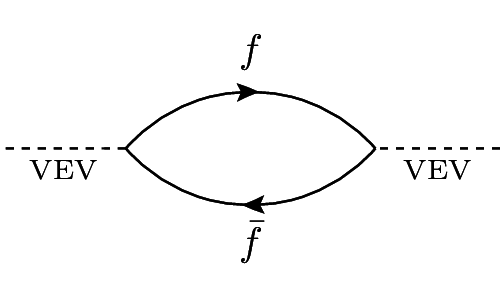
\includegraphics[width=0.5\linewidth]{figures/SM/VevFermionLoop.png}
}
\subfloat[]{
  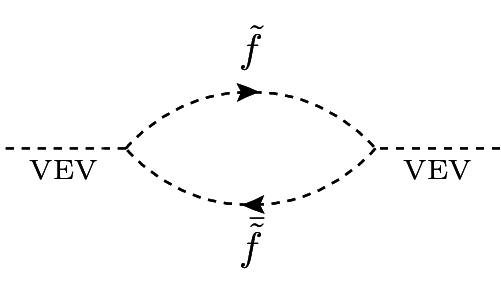
\includegraphics[width=0.5\linewidth]{figures/SUSY/VevSfermionLoop.png}
}
}
\caption{The cancelation.} 
\label{fig:SusyCancelations}
\end{figure}

But before $\SUSY$ can be seriously considered as a potential candidate, we must deal with the fact that the viability of a supersymmetric hypothesis in our universe faces two serious obstacles. They are:
\begin{enumerate}
\item{A supersymmetric $\sm$ could result in the proton being unstable.}
\item{Supersymmetry has not been observed in any experiment before.}
\end{enumerate}
Perhaps it is best to deal with these one by one.

\noindent
1. If supersymmetric interactions existed, protons would quickly decay because $\SUSY$ introduces interactions that break the accidental $\sm$ symmetries that conserve baryon and lepton numbers. Two quarks inside the proton could annihilate to form a lepton superpartner (slepton), and the proton would fly to pieces after a period of a few seconds to a year. However, experiments \cite{Miura:2009yma} have determined that the proton lifetime is greater than $10^{32}$ years, so clearly there is a spectacular discrepancy to be resolved. The situation can most easily be remedied by introducing an additional $\ztwo$ symmetry called $R$-parity \cite{Farrar:1982te}, which, as shown in Section \ref{sec:withztwo}, requires that superpartners always be produced or annihilate in pairs. This forbids the vertices involved in the proton's decay, thereby preserving proton stability. It should be noted that $R$-parity is not simply an ad hoc symmetry, but arises naturally out of many grand unification theories like SO(10), as well as out of continuous gauge symmetries that conserve B$-$L.

\noindent
2. If the $\sm$ exhibited an unbroken $\SUSY$, the masses of the superpartners would be identical to the masses of $\sm$ particles, and the superpartner of the electron would have been discovered perhaps a century ago. Supersymmetry has not been observed in any experiment so far; therefore, in order to be a viable hypothesis, it must be that the superpartners are much heavier than their $\sm$ counterparts, somehow. This can be arranged, so long as $\SUSY$ is a so-called ``softly'' broken symmetry, meaning that a certain set of terms can be added to the Lagrangian that violate $\SUSY$ by giving extra mass to the superpartners.

The fact that $\SUSY$ must be broken should not be taken as a strike against the hypothesis; as discussed in Section \ref{chap:SM}, the $\sm$ is already host to a very important symmetry that happens to be broken, namely, the electroweak $U(1)\times SU(2)$ symmetry.

As stated, even a broken $\SUSY$ will cure the $\sm$'s hierarchy problem, as long as the $\SUSY$ is only broken by a certain class of terms. Generically, these terms are of the form

\begin{equation}
\mathcal{L}_{SOFT}={\color{red}-\frac{1}{2}M_a\tilde{\lambda}_a\tilde{\lambda}_a}
{\color{Green}-\frac{1}{6}b_{ijk}\tilde{f}_i\tilde{f}_{j}\phi_k}
{\color{blue}-\frac{1}{2}b_{ij}\tilde{f}_i\tilde{f}_j}
{\color{orange}-m^2_{ij}\tilde{f}_{j}^*\tilde{f}_i}.
\label{eq:SoftBreak}
\end{equation}
The $\tilde{\lambda}$'s are the superpartner fields of gauge bosons (gauginos), the $\tilde{f}$'s are the superpartner fields of fermions (sfermions), and the $\phi$'s are scalar fields; repeated indices within a term imply a summation over species. The red and blue terms are responsible for endowing the superpartners with mass, and are needed to explain why $\SUSY$ so far has never been observed, solving problem 2. The green terms indicate the scalar trilinear interactions, and the orange are called the non-holomorphic terms~\cite{Peskin:1995ev}, which don't play a large role in this investigation but are included for completeness. I'll now explain how $\SUSY$, along with this generic set of soft breaking terms, could be realized in the the context of the $\sm$.

\section{The MSSM}
\label{sec:mssm}
Introducing supersymmetry into the $\sm$ yields the set of supermultiplets listed in Table \ref{tab:MSSM}. You'll notice that there are two Higgs supermultiplets. The reason, in short, is that $\SUSY$ requires there to be a second Higgs doublet to prevent an electroweak gauge anomaly \cite{Martin:1997ns}. Represented here are the fields that make up the minimal supersymmetric $\sm$ (MSSM), which predicts the existence of 41 extra fields in addition the 33 fields of the $\sm$. That is 33 superfields matching to the known $\sm$ fields, and eight new fields arising from the second Higgs doublet. The supersymmetric Lagrangian containing these fields is given by
\begin{align}
W_{MSSM}=\bar{u}\textbf{y$_d$}QH_u-\bar{d}\textbf{y$_d$}QH_d-\bar{e}y_eLH_d+\mu H_uH_d.
\end{align}

Table \ref{tab:MSSM} summarizes the fields of the MSSM before symmetry breaking.
\begin{table}
\begin{centering}
\caption{The supermultiplets of the MSSM. }
\begin{tabular}{  l | c | c | c | c}
\hline
\hline
Supermultiplets & spin 0 & spin 1/2 & spin 1 & number of fields/2 \\
\hline
\multirow{2}{*}{Higgs, Higgsino} & $H_u$  & $\tilde{H}_u$ &  & 2 \T\B\\
& $H_d$ & $\tilde{H}_{d}$ &  & 2 \T\B\\ 
\hline
& $\tilde{Q}_L$ & $Q_L$ &  & 6 \T\B\\
quark, squark& $\tilde{u}_{R}^*$ & $u_{R}^\dag$ &  & 3 \T\B\\
& $\tilde{d}_{R}^*$ & $d_{R}^\dag$ &  & 3 \T\B\\
\hline
\multirow{2}{*}{lepton, slepton} & $\tilde{L}_L$ & $L_L$ &  & 6 \T\B\\
& $\tilde{e}_{R}^*$ & $e_{R}^\dag$ &  & 3 \T\B\\
\hline
B boson, bino &  & $\tilde{B}$ & $B$ & 1 \T\B\\
W boson, wino &  & $\tilde{W}$  & $W$ & 3 \T\B\\
gluon, gluino &  & $\tilde{g}$ & $g$ & 8 \T\B\\
\hline
\hline
\end{tabular}
\label{tab:MSSM}
\end{centering}
\end{table}
As discussed, an unbroken supersymmetric $\sm$ doesn't exist. Therefore, to complete the description of the MSSM, the generic soft-breaking Lagrangian in Equation \ref{eq:SoftBreak} must be expressed in terms of the specific superfields listed in Table \ref{tab:MSSM}. Suppressing the chirality labels, one obtains
\begin{equation}
\begin{split}
\mathcal{L}_{\text{SOFT},\,\text{MSSM}}=
&{\color{red}-1/2(M_1\tilde{B}\tilde{B}+M_2\tilde{W}\tilde{W}+M_3\tilde{g}\tilde{g})}\\
&{\color{Green}-\tilde{\bar{u}}\hat{\textbf{a}}_u\tilde{Q}H_u-\tilde{\bar{d}}\hat{\textbf{a}}_d\tilde{Q}H_d-\tilde{\bar{e}}\hat{\textbf{a}}_e\tilde{Q}H_d}\\
&{\color{blue}-\tilde{Q}^\dag\hat{\textbf{m}}_{Q}^2\tilde{Q}-\tilde{L}^\dag\hat{\textbf{m}}_{L}^2\tilde{L}-\tilde{\bar{u}}\hat{\textbf{m}}_{u}^2\tilde{\bar{u}}^\dag-\tilde{\bar{d}}\hat{\textbf{m}}_{d}^2\tilde{\bar{d}}^\dag}\\
&{\color{blue}-\tilde{\bar{e}}\hat{\textbf{m}}_{e}^2\tilde{\bar{e}}^\dag-bH_uH_d}\\
&{\color{orange}-m^2_{H_u}H_u^*H_u-m_{H_d}^2H_d^*H_d},
\end{split}
\label{eq:SoftBreakMSSM}
\end{equation}
where the bold hatted symbols are complex $3\times3$ matrices in family space, and colors show the correspondence between similar terms in Equations \ref{eq:SoftBreak} and \ref{eq:SoftBreakMSSM}. In total, Equation \ref{eq:SoftBreakMSSM} contains 107 unknown parameters \cite{Dimopoulos:1995ju}, which along with the four parameters from the second Higgs doublet, span the 111 unknown free parameters of the MSSM. That is 111 new parameters that must in principle be measured in future experiments, if the MSSM is indeed a model that describes nature.

Unfortunately, the large number of free parameters renders the MSSM parameter space impossible to explore exhaustively, at least for now. But, the vast set of experimental observations collected at particle physics experiments over decades, as well as theoretical motivations, can be used to constrain the model space, and make studying the MSSM a possibility. A number of constrained submodels of the MSSM have been developed and studied, two of which are discussed now.

\section{The cMSSM}
The constrained MSSM, or cMSSM \cite{Wess:1984jr}, is a well-named submodel of the MSSM that makes many assumptions about the MSSM. This reduces enormously the dimensionality of the model. Sufficient assumptions are made to reduce the number of $\SUSY$ breaking parameters from 107 to just five. Central to these defining assumptions is the idea that at some energy near the GUT scale ($10^{16}$ GeV), the superpartners become mass degenerate, a feature motivated by certain grand unification scenarios. This allows for all the sfermion masses to be set to a single value at the selected high energy, and the same for the gaugino and Higgsino masses, that is,
\begin{align}
{\color{red}M_3}={\color{red}M_2}={\color{red}M_3} & \equiv m_{1/2},\\
{\color{blue}\hat{\textbf{m}}_Q^2}={\color{blue}\hat{\textbf{m}}_L^2}={\color{blue}\hat{\textbf{m}}_u^2}={\color{blue}\hat{\textbf{m}}_d^2} ={\color{orange}m_{H_u}^2\mathds{1}}={\color{orange}m_{H_d}^2\mathds{1}}& \equiv m_0^2\mathds{1},\\
{\color{Green}\hat{\textbf{a}}_{u,d,e}} & \equiv A_0\cdot{\color{cyan}y_{t,b,\tau}} \eightZeroMat,\\
{\color{blue}b} & \equiv B_0\cdot \text{sign}(\mu).
\end{align}
The five black symbols on the right hand side, $m_{1/2}$, $m_0$, $A_0$, $B_0$, and sign($\mu$) are the
free parameters of the cMSSM, and the cyan $y_{t,b,\tau}$ are the known $\sm$ values of weak hypercharge for the top quark, bottom quark, and tau lepton. Because most of these are matrix equations, there are many more constraints than equations; 102 constraints to be specific. As mentioned, the cMSSM has very low dimensionality, and as a result, the model can be readily used to interpret experimental data. However, most of the constraints responsible for the reduction in dimensionality are not particularly well motivated, as they amount to assumptions about the laws of physics at scales that have never been observed by humans. Furthermore, any conclusions made about the cMSSM based on data collected in particle experiments are highly contingent, since only a tiny fraction of the phenomenological possibilities within the MSSM are realized in the cMSSM.

This is not to say that models like the cMSSM have not played an important role in the evolution of our understanding of $\SUSY$. They have provided benchmarks against which to compare the past and present sensitivity of experiments that probe supersymmetric hypotheses. They may play an increasingly important role in the future, if a significant part of the superpartner spectrum is discovered, and hints of the true $\SUSY$ breaking mechanism begins to appear. Such a breaking scheme could be quite elegant, described by only a few independent parameters. That said, very constrained models that make many untested assumptions are less useful when, as yet, there is absolutely no hint of supersymmetry.

\section{The pMSSM}
\label{sec:pmssm}
The phenomenological MSSM (pMSSM) is another submodel of the MSSM, one based on far fewer assumptions than the cMSSM. In particular, the pMSSM makes no assumption about how the $\SUSY$ breaking parameters are related at the GUT scale. The pMSSM~\cite{Berger:2008cq} was developed with the aim of making as few assumptions about the MSSM as possible, while reducing the size of the model's parameter space to a level that is practicable and workable. The assumptions defining the pMSSM are:
\begin{itemize}
\item{there are no new flavor changing neutral currents;}
\item{there are no new sources of CP violation at tree level;}
\item{the first and second generation fermions masses are degenerate, and}
\item{the lightest of the superpartners is the neutralino.}
\end{itemize}
The first two assumptions are motivated by the observation that CP-violating processes are extremely rare, even at loop level (higher order than tree-level), and flavor changing neutral currents are not observed at all. The third assumption is borne of the expectation that a model with two independent fermion generations will be as phenomenologically complete as a model with three generations, particularly in the early phases of discovery when only part of the full superpartner spectrum has been detected. The final assumption ensures that the lightest superpartner is electrically neutral, which is strongly motivated by cosmological observations. This leaves the following 19 parameters free:
\begin{itemize}
\item{three gaugino mass parameters {\color{red}$M_1$}, {\color{red}$M_2$}, and {\color{red}$M_3$};}
\item{one higgsino mass parameter $\mu$ and one pseudo-scalar Higgs mass $m_A$;}
\item{ten sfermion mass parameters {\color{blue}$m_{\tilde{f}}$}, where $\tilde{f}=\tilde{Q}_1$, $\tilde{U}_1$, $\tilde{D}_1$, $\tilde{L}_1$,  $\tilde{Q}_3$, $\tilde{U}_3$, $\tilde{D}_3$, $\tilde{L}_1$, and $\tilde{E}_3$ (imposing $m_{\tilde{Q}1}=m_{\tilde{Q}2}=m_{\tilde{L}1}=m_{\tilde{L}2}$);}
\item{three trilinear couplings {\color{Green}$A_t$}, {\color{Green}$A_b$}, and {\color{Green}$A_\tau$}, and}
\item{the ratio of the two Higgs vacuum expectation values $\text{tan}(\beta)=\text{VEV}_A/\text{VEV}_h$.}
\end{itemize}
With the particle masses free to vary independently throughout the model space, the pMSSM captures most of the possible, experimentally relevant phenomenology of the MSSM.  Despite the still rather large dimensionality of 19 free parameters, the model has been successfully used for the interpretation of experimental results, as demonstrated in ``The pMSSM interpretation of CMS 7 and 8 TeV results'' \cite{Khachatryan:2016nvf}, as well as in \cite{Carena:2012he, Aad:2015baa}. An detailed account is given in Chapter \ref{chap:run1pmssm}.

\section{Dark matter candidate}
If $\SUSY$ is realized in Nature in the context of the $\sm$, and if $R$-parity is conserved, there exists a new heavy stable particle, called the LSP (lightest supersymmetric particle). If this particle is electrically neutral and colorless, it matches the criteria necessary to be dark matter. There are several such candidates, including the superpartners of Higgs boson, the Z boson, and the photon. This possibility serves as an additional motivation for searching for $\SUSY$ in particle colliders. 

\chapter{The Large Hadron Collider}
\label{chap:lhc}
The world's foremost tool for observing physics at the electroweak scale is a particle accelerator and collider facility called the Large Hadron Collider (LHC) \cite{Breskin:1244506}. Located at the European Organization for Nuclear Research (CERN) in Geneva, Switzerland, the LHC is the largest and perhaps most complex machine ever constructed, and the source of the world's most energetic laboratory-prepared particles. This machine offers our best chance of observing evidence of new structure that may describe our universe at the smallest scales, including perhaps the particles and fields of \SUSY.

\section{LHC key features}
The primary feature of the LHC is a meter-wide, 26.7 kilometer-long cryogenic vacuum cylinder forming a nearly circular path below ground in France and Switzerland. The LHC ring occupies a 4 meter-wide tunnel whose depth ranges between 45 and 170 meters beneath the surface. During normal operation, the LHC ring houses two counter-circulating beams of energetic protons, which are steered by superconducting magnets and brought to intersect at various points around the ring. There are four such crossing points, located at the centers of the four LHC experiments, ATLAS, ALICE, CMS, and LHC-b, where high energy protons collide. The layout of the LHC is shown in Figure \ref{fig:LHCLayout}. 

\begin{figure}[t]
\centering
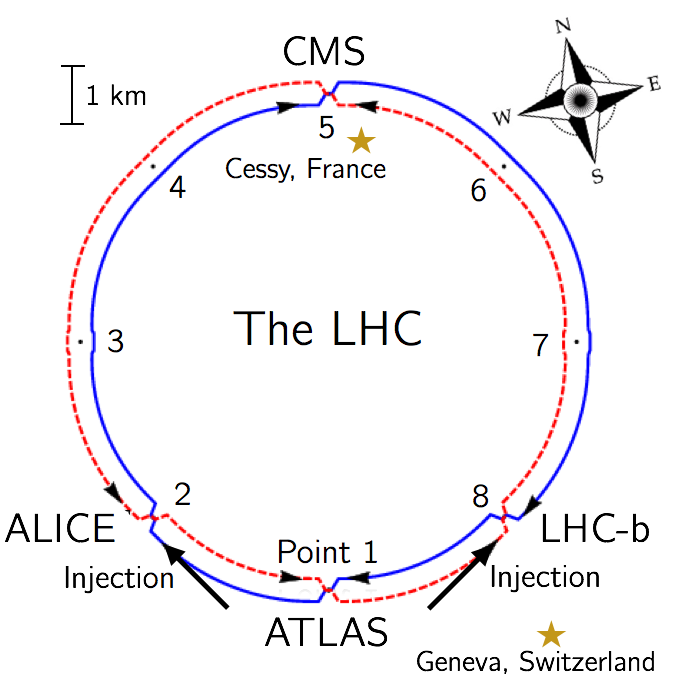
\includegraphics[width=.75\linewidth]{figures/LHC/LHC.png}
\caption{The layout of the Large Hadron Collider. The scale is approximate and the separation between the beams has been exaggerated to show the crossings of beam 1 (blue) and beam 2 (red) at interaction points 1, 2, 5, and 8.} 
\label{fig:LHCLayout}
\end{figure}

The LHC ring does not form a perfect circle, but rather is made of alternating curved and straight sections. The curved sections are 2500 meters long in arc length and are instrumented with superconducting dipole magnets. The straight sections are 530 meters long, and their centers (labeled as points 1-8 in Figure \ref{fig:LHCLayout}) have either been instrumented with hardware that serves necessary functions for the operation of the LHC, or with of the experimental facilities. 

The hardware and functionality of each of the LHC's eight points is summarized in Table \ref{tab:LHCPoints}.  The primary experimental facilities, mentioned above, observe high energy proton and heavy ion collisions and perform both $\sm$ measurements and searches for BSM physics. In addition to the four primary experiments, Table \ref{tab:LHCPoints} lists in parentheses a few additional experimental facilities that share interaction points with the primary four. TOTEM shares the experimental cavern with CMS on the LHC ring at point 5 and measures, among other observables, proton-proton elastic scattering cross sections; MOEDAL shares the interaction point 8 with LHC-b and performs searches for particles with magnetic monopole moments, and LHC-f is a future experiment that will share interaction point 1 with ATLAS and study particles that travel nearly parallel with the beam direction (the forward direction).


\begin{table}
\begin{centering}
\begin{tabularx}{\textwidth}{>{\setlength\hsize{0.11\hsize}\setlength\linewidth{\hsize}}X|>{\setlength\hsize{.45\hsize}\setlength\linewidth{\hsize}}X|>{\setlength\hsize{.7\hsize}\setlength\linewidth{\hsize}}X}
\hline
\hline
point & hardware & functionality \\
\hline
\vspace{-3.00mm} 1 & \vspace{-3.00mm} ATLAS experiment \cite{Aad:2012naa}& 
\vspace{-7.5mm}
\begin{itemize}
\item full coverage particle detector
\item proton-proton collisions
\item performs \SM~measurements and performs searches for evidence of new particles
\end{itemize}\\
&\vspace{-4mm}LHC-f experiment \cite{Adriani:2008zz}&
\vspace{-7mm}
\begin{itemize}
\item forward particle detector
\end{itemize}\\
\hline
\vspace{-3.00mm} 2 & \vspace{-3.00mm} ALICE experiment \cite{Leistam:644017}& 
\vspace{-7.5mm}
\begin{itemize}
\item partial coverage particle detector
\item heavy ion collisions
\item studies the \SM~and performs searches for new particles
\end{itemize}\\
\hline
\vspace{-3.00mm} 3 & \vspace{-3.00mm} RF cavities & 
\vspace{-7.5mm}
\begin{itemize}
\item momentum cleaning
\end{itemize}\\
\hline
\vspace{-3.00mm} 4 & \vspace{-3.00mm} sextupole magnets & 
\vspace{-7.5mm}
\begin{itemize}
\item acceleration
\end{itemize}\\
\hline
\vspace{-3.00mm} 5 & \vspace{-3.00mm} CMS experiment \cite{Chatrchyan:2008aa}& 
\vspace{-7.5mm}
\begin{itemize}
\item full coverage particle detector
\item proton-proton collisions
\item performs \SM~measurements and performs searches for new particles
\end{itemize}\\
\vspace{-0.0cm}
&\vspace{-4mm}TOTEM  experiment \cite{Anelli:2008zza}&
\vspace{-7mm}
\begin{itemize}
\item forward particle detector
\end{itemize}\\
\hline
\vspace{-3.00mm} 6 & \vspace{-3.00mm} quadrupole magnets & 
\vspace{-7.5mm}
\begin{itemize}
\item beam focusing
\end{itemize}\\
\hline
\vspace{-3.00mm} 7 & \vspace{-3.00mm} sextupole magnets & 
\vspace{-7.5mm}
\begin{itemize}
\item betatron cleaning
\end{itemize}\\
\hline
\vspace{-3.00mm} 8 & \vspace{-3.00mm} LHC-b experiment \cite{Alves:2008zz}& 
\vspace{-7.5mm}
\begin{itemize}
\item partial coverage particle detector
\item heavy ion collisions
\item studies the \SM~and searches for evidence of new particles
\end{itemize}\\
&\vspace{-4mm}\small MOEDAL\normalsize~experiment~\cite{Pinfold:2015laa}&
\vspace{-7mm}
\begin{itemize}
\item forward physics
\end{itemize}\\
\hline
\hline
\end{tabularx}
\caption{The hardware at the interaction points of the LHC.}
\label{tab:LHCPoints}
\end{centering}
\end{table}

Figure \ref{fig:BeamCS} shows a typical cross section of the LHC ring. Within the outer steel casing are not only the two proton beams, but also the magnets and other instrumentation required to control and manipulate the beams. A continuous ultra high vacuum is maintained in the outer volume in order to thermally insulate the inner volume. The inner volume is filled with an iron yoke and held at a temperature of 1.9 K by supercooled liquid helium, which flows through the heat exchanger pipe. Inside the yoke and in thermal equilibrium with the iron is a twin bore assembly of niobium titanium superconducting coils that produce magnetic fields with strengths of up to 9 Tesla (T). Within the focus of the coils are the two parallel evacuated beam pipes, highways for subatomic particles.


\begin{figure}[t]
\centering
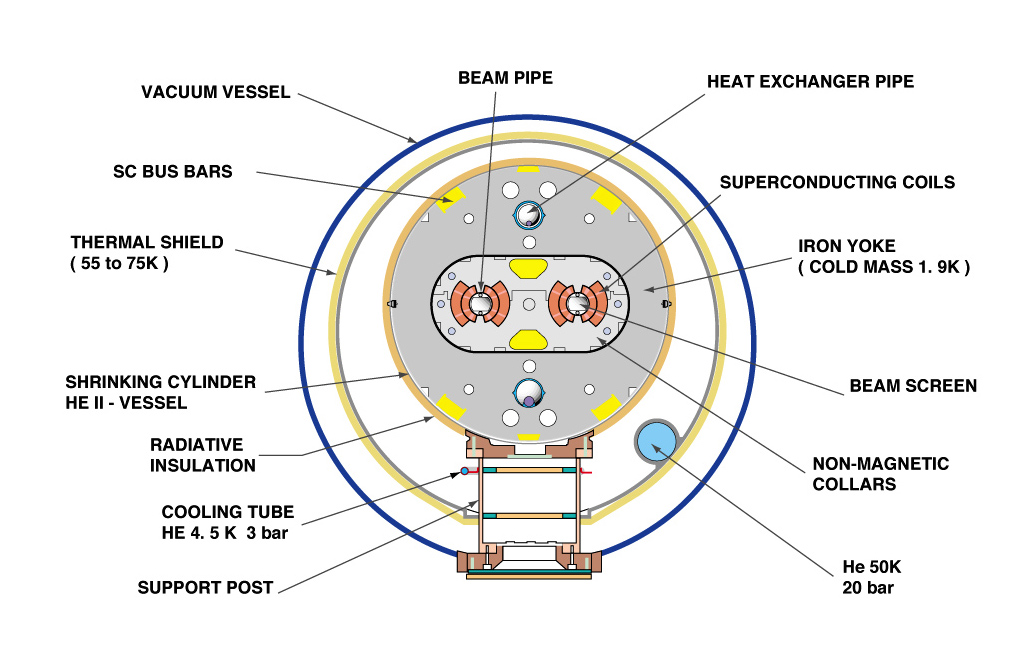
\includegraphics[width=1.0\linewidth]{figures/LHC/LHCDipole.jpg}
\caption{Cross section of a cryodipole, the most common segment of the LHC \cite{Jean-Luc:841539}. } 
\label{fig:BeamCS}
\end{figure}


The LHC's superconducting coils produce various magnetic field geometries to serve different functions. About 1200 cryodipole magnets are positioned in the curved LHC segments and produce dipole fields that bend the protons along their arched trajectories;  about 400 magnets located in the LHC's short straight sections produce quadrupole fields that are used to focus the beams, and thousands of additional magnets produce sextupole, octopole and decapole fields that purify and adjust the beams in various ways. 

Additional systems are responsible for the refrigeration of liquid helium, the powering and protection of the superconducting coils, and the maintenance and dumping of the particle beams. 

\section{The injection sequence}
Long before they reach the LHC beam pipes, protons are accelerated and focused by a multi-staged process. Initially the protons are stored as the nuclei of gaseous hydrogen atoms, kept in a sealed bottle at the CERN accelerator complex. When the LHC operators begin the procedure of filling the machine with protons, the hydrogen in the bottle is injected into a duoplasmatron~\cite{Breskin:1244506}, which subjects the hydrogen to an electric field and a bombardment of electrons. The electrons ionize the hydrogen atoms, and the electric field carries the liberated hydrogen nuclei (protons) through the duoplasmatron cavity, providing them with 100 keV of kinetic energy. Upon leaving the duoplasmatron, the protons are gathered by a quadrupole magnet and guided into the aperture of a linear accelerator called LINAC2, where they are accelerated by radio frequency (RF) cavities up to an energy of 50 MeV. LINAC2 discharges the protons into a cyclotron called the Proton Synchrotron Booster (PSB), which accelerates the protons repeatedly as they cycle around a 20-meter circular path. After reaching an energy of 1.4 GeV within the PSB, the protons are injected into a larger cyclotron called the Proton Synchrotron (PS). The PS elevates the protons' kinetic energy to 25 GeV before passing them to the world's second largest particle accelerator, the Super Proton Synchrotron (SPS), which takes the protons up to an energy of 450 GeV. The energy is now high enough for the protons to be injected into the LHC. 

Protons are injected into the LHC at 450 GeV and accelerated up to the highest energy ever achieved at a laboratory, 6.5 TeV. The beams are collided head-on, yielding a collision energy of 13 TeV in the proton-proton center of mass frame. To understand why it is necessary to push the energy frontier in this way, it is necessary to explain the goals of the LHC.


\section{The goals of the LHC}
One of the goals of the LHC is to produce and observe new, heavy particles in the collisions of protons. This of course assumes that such particles actually exist. Assuming they exist, and for concreteness, that the new particles are the particles of \SUSY, there are two main ingredients required to produce \susy~particles, both of which can be understood by examining the expression that governs how many proton-proton collisions are expected to result in the creation of \susy~particles:
\begin{equation}
N_{\rm SUSY} = \lumi\cdot \sigma_{\rm SUSY}.
\end{equation}
Here, $N_{\rm SUSY}$ is the number of events in which \susy~particles are present, where ``event'' is defined as the collection of particles emanating from a single collision. The quantity $\sigma_{\rm SUSY}$ is the interaction cross section, a measure of the probability for a supersymmetric interactions to occur during a collision
\begin{equation}
\sigma_{\rm SUSY} = \sum_{f}|M_{fi}|^2,
\end{equation}
where the sum runs over all final states $\ket{f}$ containing supersymmetric particles, and $|M_{fi}|$ is the amplitude (Section \ref{sec:Amp}) for a system to evolve from an initial state $\ket{i}$ containing two incoming protons into the given final state $\ket{f}$. The symbol $\lumi$ stands for the integrated luminosity, and is a measure of the total number of protons collided:
\begin{equation}
\lumi = \frac{N_{\rm collisions}}{\sigma_{\rm pp}}.
\end{equation} 
Here, $N_{\rm collisions}$ is the total number of collisions achieved at the LHC and $\sigma_{\rm pp}$ is the cross section for protons to interact. Clearly, since the goal is to maximize $N_{\rm SUSY}$, it is important to maximize both $\sigma_{\rm SUSY}$ and $\lumi$. The maximization of $\sigma_{\rm SUSY}$ is achieved by imparting as much kinetic energy as possible to the protons.  The maximization of $\lumi$ is achieved by making the beam intensities, i.e., the number of protons per unit volume and time as possible. A few details on these two objectives are now given.

\subsection{The objective of high energy}

Owing to energy conservation, the probability of producing a supersymmetric particle gets lower as the hypothetical mass of the particle increases.  However, this limitation can be overcome by increasing the energy of the colliding protons. In other words, $\sigma_{\rm SUSY}$, and thus $N_{\rm SUSY}$, increase as a function of the proton energy. This is why the primary objective of the LHC is to achieve high energy collisions.


\subsection{The objective of high luminosity}
While high energy is the primary goal of the LHC, the other essential goal is to provide as large a beam intensity as possible. This is achieved by maximizing $N_{\rm collisions}$, by colliding as many protons as possible within a given period of time. To this end, the proton beams are not continuous beams, but are segmented into bunches, which are groups of a few billion protons, where the bunches are spaced apart in time intervals of 50 ns (25 ns) in Run 1 (Run 2). Maximizing the number of observed collisions is important because new physics processes are expected to be very rare, and as few as one in 10 billion collisions might contain the kind of new physics that is being looked for. The design luminosity of the LHC is $\mathcal{L}=10^{34}$ cm$^{-2}$s$^{-1}$.


\chapter{The Compact Muon Solenoid}
\label{chap:cms}
Centered at collision point 5 of the LHC, and located 100 meters below the town of Cessy, France, is an underground cavern that houses a particle detector called the Compact Muon Solenoid (CMS)~\cite{Breskin:1244506}~\cite{Chatrchyan:2008aa}. Weighing 12,500 tonnes and occupying a volume of 3600 cubic meters, CMS (shown in Fig. \ref{fig:CmsPulledApart}) is the most massive particle detector to be constructed at a collider experiment. The experimental collaboration that built, operates and uses the data collected by the detector is called the CMS collaboration, and comprises over 3000 participants from 199 institutions in 43 countries. 

The CMS detector was designed to study, among other things, particles produced through rare electroweak processes. At the LHC, such processes occur amid an overwhelming number of QCD dijet events (events with two  hadronic showers that recoil back-to-back) in an environment of high instantaneous luminosity. To reconstruct and identify particles amid the large background, the various sub-detectors of CMS measure various properties of the particles emerging from the collisions, and this information is used to form particle candidates. The properties that can be measured include the electric charge, energy, momentum, direction of motion, particle identity (ID), and the decay lifetime of particles. The ability to use information from the various sub-detectors to identify and characterize individual particles is made possible by CMS's fine granularity, meaning the sub-detectors are composed of small, closely-spaced units, or cells. The fine granularity is key to accurately measuring the position of particles passing through the detector, and minimizing the chances that the same cell will be activated by two particles simultaneously, which can complicate the reconstruction. This complication is enhanced by the fact that the high instantaneous luminosity of the LHC leads to, in most cases, the occurrence of multiple simultaneous collisions per bunch crossing rather than just a single collision, an effect called pile-up. A precise determination of the momentum of particles is made possible by a high magnetic field that fills the space of the inner sub-detectors, the tracker and electromagnetic calorimeter, described below. The global analysis of each event and its constituent particles is performed by an algorithm called particle flow \cite{Beaudette:2014cea}, some details of which are provided in the sections below.

\begin{figure}[h]
\centering
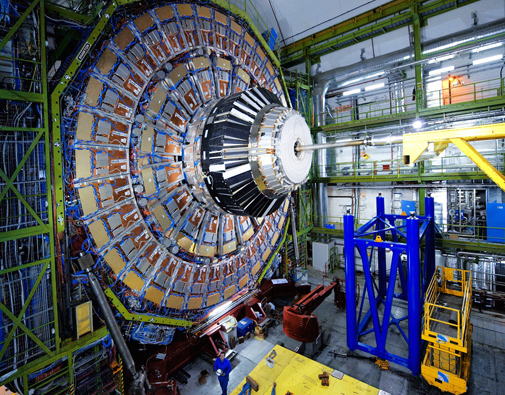
\includegraphics[width=0.6\linewidth]{figures/CMS/CMSBetter.jpg}
%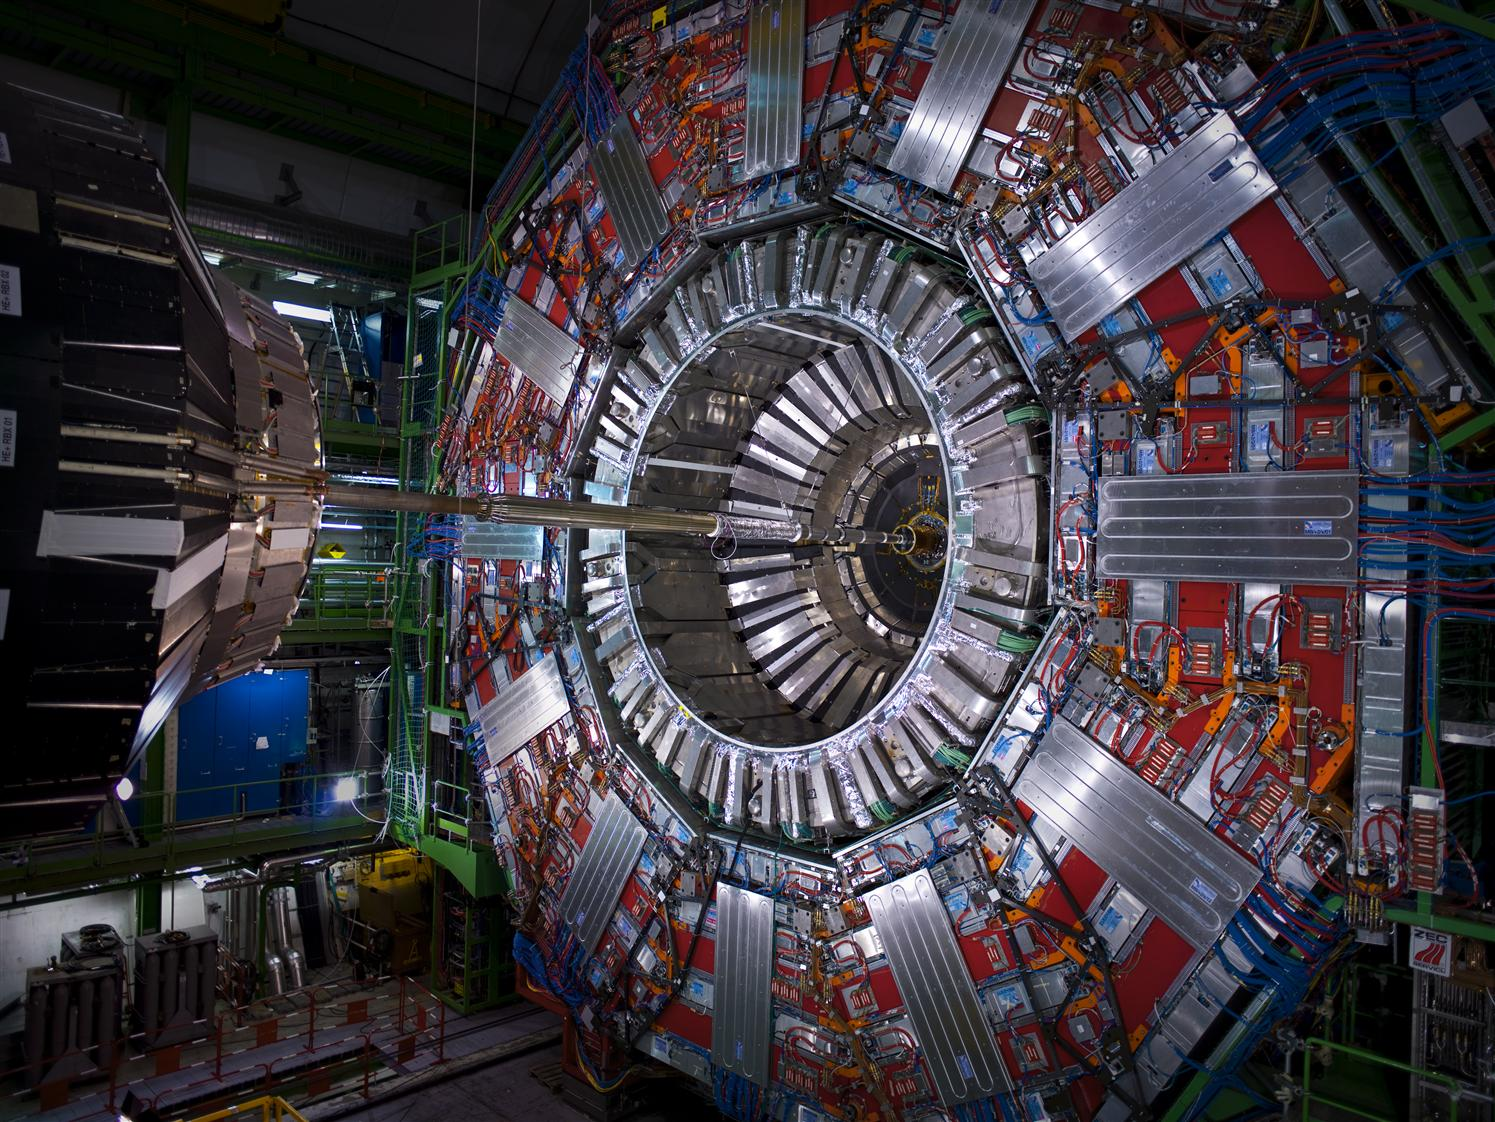
\includegraphics[width=1.0\linewidth]{figures/CMS/CMS1.jpg}
\caption{The CMS detector, pulled apart during the long shutdown of 2014. } 
\label{fig:CmsPulledApart}
\end{figure}
A photograph of the CMS detector is given in Fig. \ref{fig:CmsPulledApart}. The sub-detectors are nested cylindrically around the LHC beams, centered on the interaction point. A description of the coordinate system used by CMS, as well as a set of key observables that CMS is capable of reconstructing, is given in the following section. Then, the main systems are described, starting from the inside (closest to the beam lines) and moving outward.

\section{Coordinates and observables}
The CMS detector makes use of both a right-handed cartesian coordinate system as well as an approximately Lorentz invariant spherical coordinate system (HEP coordinate system). In the cartesian system, $\hat{x}$ points toward the center of the LHC, $\hat{y}$ points up, and $\hat{z}$ points in the direction of the counterclockwise rotation of the LHC beam pipe as viewed from above. The HEP coordinate system is spanned by the basis vectors $\pt$ (transverse momentum), $\eta$ (pseudorapidity), and $\phi$ (azimuthal angle), which translate to the right-handed cartesian coordinate system through the relations:
\begin{align}
\pt &= \sqrt{(p_{x})^2+(p_{y})^2}\\
\eta &= -\text{ln}[\text{tan}(\theta/2)]\\
\phi &= \hphantom{-}\text{tan}^{-1}(p_{\text{y}}/p_{\text{x}}),
\end{align}
where $\theta$ is the polar angle from the positive $\hat{z}$ axis.

The missing transverse momentum $\METvec$ is defined as the negative of the vector sum of the momenta of all visible particles in an event, projected on the plane transverse to the beam:
\begin{equation}
\METvec\!\equiv\!-\sum\limits_{i}^n(\vec{p}_T)_i.
\end{equation}
The $\METvec$ has magnitude $|\METvec|$, or just $\met$, and direction $\phimiss$, and is an estimate of the transverse momentum of the invisible particles. Since the true mass of an invisible particle is not observable, such masses are conventionally assumed to be zero, and the magnitude of the $\METvec$ vector is thus equated with the missing transverse energy \MET. The $\METvec$ can be used to construct the four-vector
\begin{equation}
(p_{\text{T}}^{\text{miss}})^\mu\equiv\!(E_T^{\text{miss}},\METvec)^\mu.
\end{equation}

Another key observable, $\Ht$, is a measure of the total hadronic energy in an event, and is defined as the scalar sum of the transverse momenta of jets in an event, or 
\begin{equation}
\Ht\!\equiv\!-\sum\limits_{i}^n(p_T)_i.
\end{equation}



\section{Silicon tracker}
The innermost system of CMS, immediately encountered by particles emerging from collisions, is the tracker \cite{Veszpremi:2014hpa}. Shown in Fig. \ref{fig:CmsTracker}, the tracker consists of two subsystems: a 600 cm-long inner pixel detector extending out to a radius of 11 cm, and a 5.8 m-long outer strips tracker extending out to a radius of 1.2 m.  The pixel detector is made of 66 million silicon pixels, and the strips detector contains 10 million silicon strips. The density of readout channels is highest within the innermost detector elements because the intensity of particle flux is highest in this region. Tracks left by muons (hadrons) are reconstructed with a very high efficiency of greater than 99\% (90\%) with a fake rate as low as 1\%, for transverse momenta as low as 150 MeV.
\begin{figure}[h]
\centering
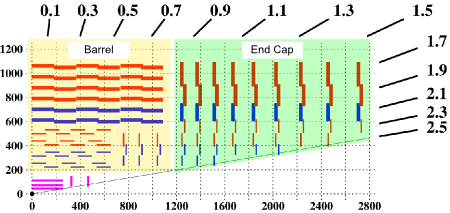
\includegraphics[width=0.75\linewidth]{figures/CMS/TrackerLayout.png}
\caption{A schematic view of the CMS tracker. The direction of view is toward the center of the LHC.} 
\label{fig:CmsTracker}
\end{figure}
At the design luminosity of the LHC of $10^{34}$ cm$^{-2}$s$^{-1}$, approximately 1,000 particles are created each 25 ns bunch crossing. This means that during the reconstruction, the innermost pixel layer is responsible for disentangling the tracks of about one million particles per mm$^2$ each second. The pixel detector is also responsible for resolving each particle's impact parameter, which is the distance of closest approach of the particle's trajectory to the point of the proton-proton collision, which is called the primary vertex. This task will be particularly challenging when the LHC enters its high luminosity phase, since the occurrence of multiple collisions within the same bunch crossing, will become much more prevalent. 

\section{Electromagnetic calorimeter}
Upon reaching the outer edge of the CMS tracker, particles enter the electromagnetic calorimeter (ECAL). The ECAL is made of 72,000 lead tungstate (PbWO$_4$) crystals, like the one shown in Fig. \ref{fig:CmsTracker}. 
\begin{figure}[h]
\centering
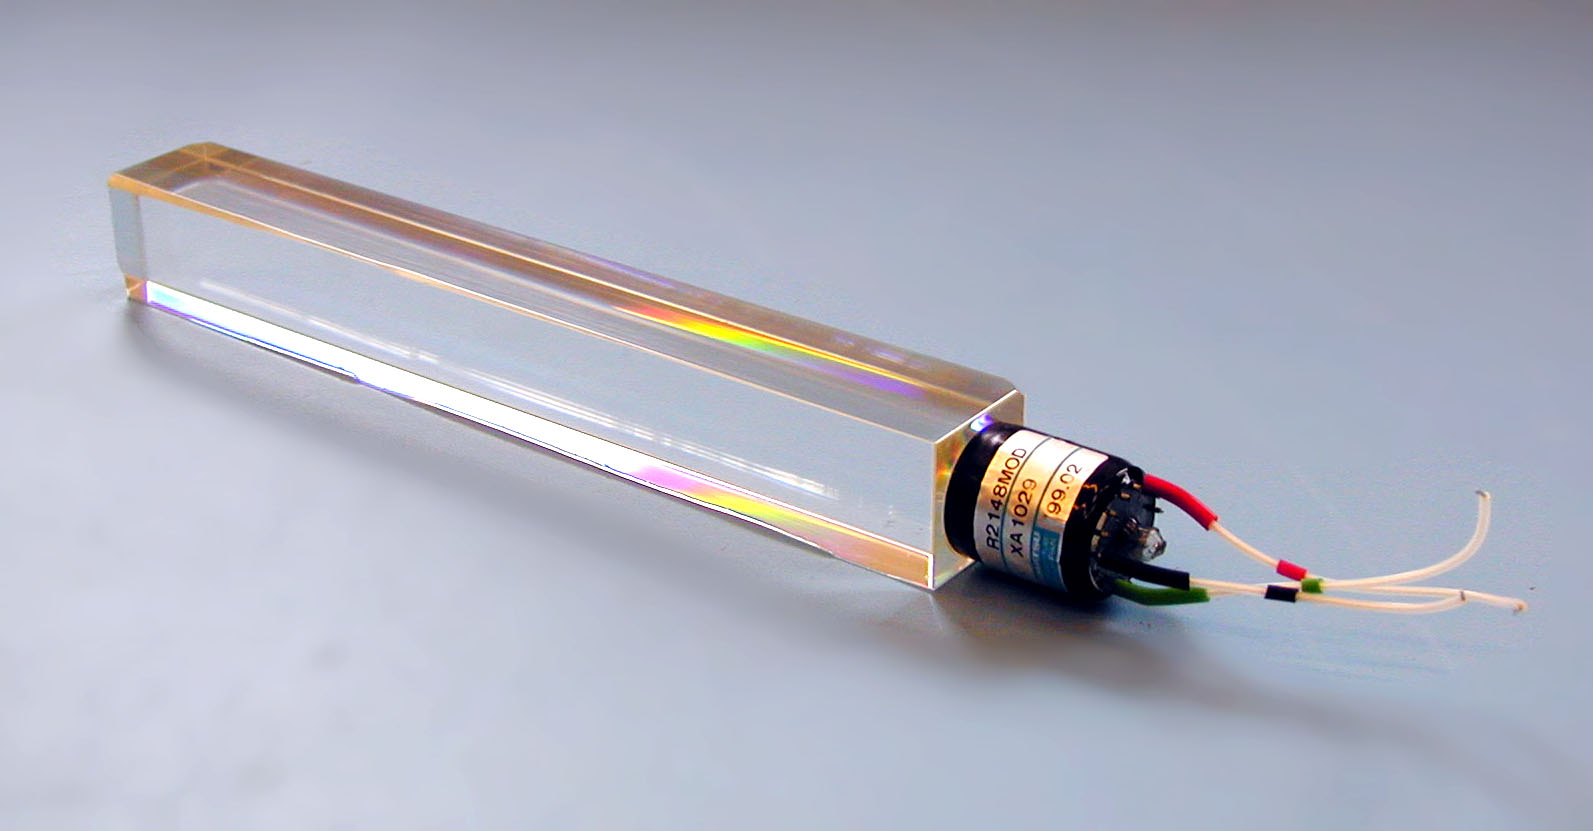
\includegraphics[width=0.75\linewidth]{figures/CMS/PbWO4.jpg}
\caption{An ECAL endcap PbWO$_4$ crystal, length 220 mm (24.7 X$_0$).} 
\label{fig:CmsTracker}
\end{figure}
The material was chosen for its high density and high optical transparency, which, respectively, guarantee a short radiation length (X$_0$ = 0.89 cm) and efficient transmission of light. Highly-relativistic charged  particles emit bremsstrahlung radiation as they traverse the crystals, resulting in electromagnetic showers, and the light is collected by photodetectors mounted on the backs of the ECAL crystals. The amount of radiation produced is proportional to the energy of traversing particles, which key to determining the energy of particles during the event reconstruction. PbWO$_4$ is also chosen for its small Moli\`{e}re radius of 2.2 cm, which results in an improved spatial resolution of particles over that possible with other materials.
\begin{figure}[t]
\makebox[\textwidth][c]{
\centering
\subfloat[]{
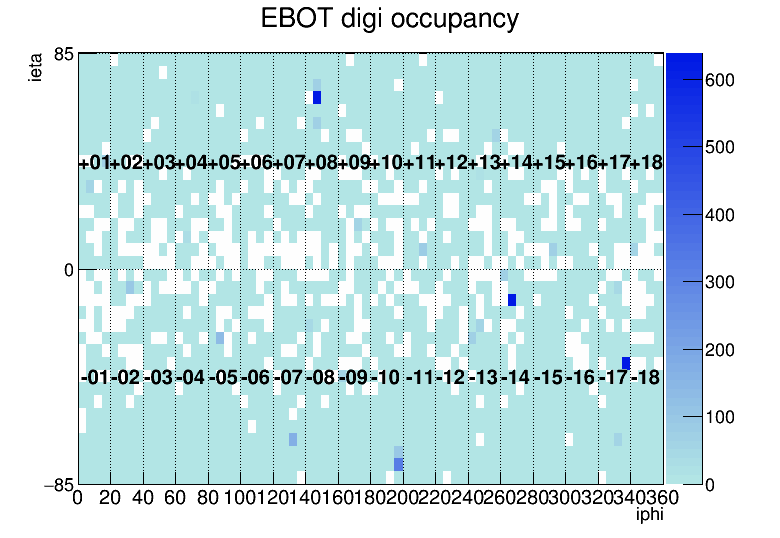
\includegraphics[width=0.7\linewidth]{figures/CMS/EBOccupancy.png}
}
}
\makebox[\textwidth][c]{
\centering
\subfloat[]{
  \vspace{2cm}
  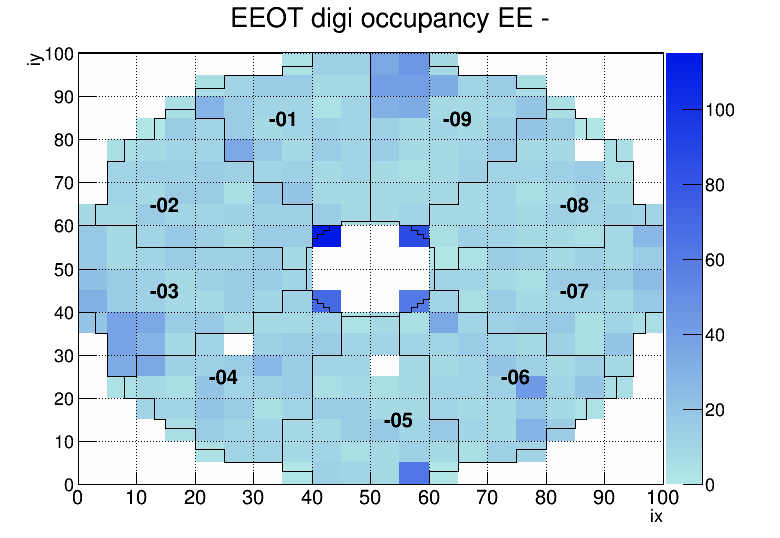
\includegraphics[width=0.5\linewidth]{figures/CMS/EB-Occupancy.png}
  }
  \subfloat[]{
  \vspace{2cm}
  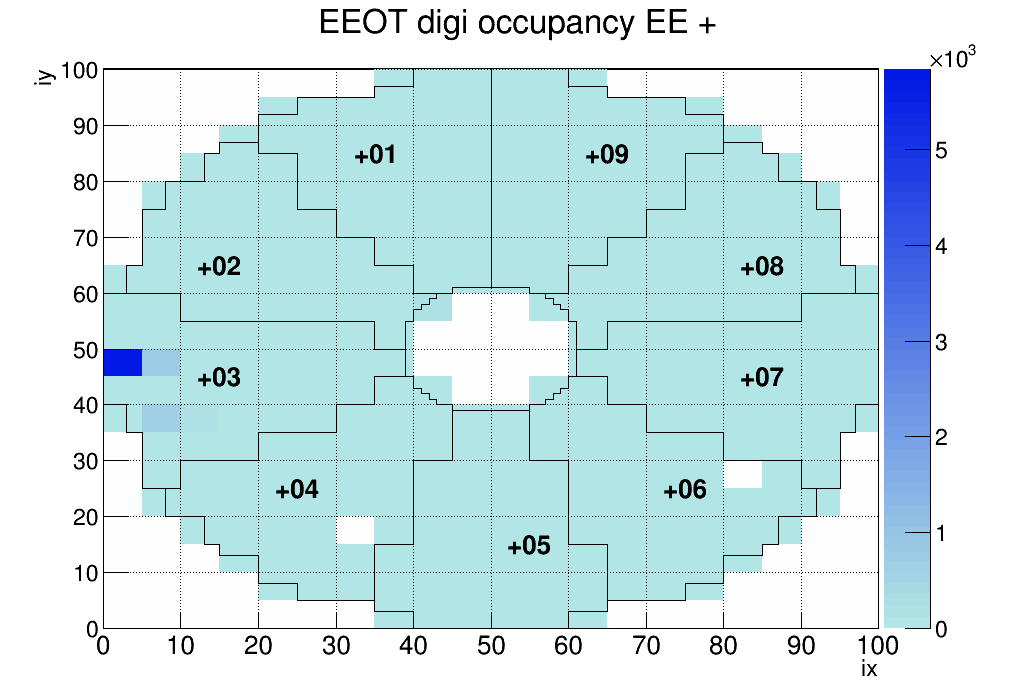
\includegraphics[width=0.5\linewidth]{figures/CMS/EB+Occupancy.png}
}
}
\caption{The layout of the ECAL barrel (a) in $\eta$-$\phi$ coordinates, and the forward (c) and rear (b) ECAL endcaps in cartesian coordinates. The shading shows the occupancy of a given run. OT stands for out-of-time, indicating that the occupancy shown in the color plot is of energy deposits that were detected out of time with the LHC bunch crossings.} 
\label{fig:EcalLayout}
\end{figure}
\FloatBarrier

In the barrel, crystals are organized into rectangular modules composed of 400 or 500 crystals each, and modules are arranged in groups of four to form supermodules. There are 36 supermodules in total, which combine to cover a large rectangular area in the space of $\eta$ and $\phi$, as shown in Fig. \ref{fig:EcalLayout} (a). This large rectangle covers all values of $\phi$ and reaches an $\eta$ of $\pm$ 1.48. In the endcaps, crystals are arranged in groups whose number varies depending on the location. The modules combine to form sectors, of which there are a total of 18, shown in Fig. \ref{fig:EcalLayout} (b) and (c). Sectors, as well as supermodules, are each read out by a front end digitizer (FED).

Deposits in the calorimeters are analyzed in the reconstruction to yield calorimeter clusters. A calorimeter cluster is composed of cells corresponding to a relative maximum in the amount of energy deposited, and the cluster energy is equal to the energy deposited in the central cell summed with the energy deposited in neighboring cells, provided that a neighboring cell has an energy deposit exceeding 1 GeV. The ECAL is capable of determining the energy of photons and electrons with a resolution of 1$-$5\%, depending on the pseudorapidity, and charged hadrons with a resolution of about 10\%. 



\subsection{ECAL calibration}
Ensuring an equivalent and accurate response among the various crystals (channels) requires a detailed calibration procedure. The ECAL is calibrated {\it in situ}, or while the detector is operating, and a number of methods are employed. The first method exploits the the principle of the $\phi$-invariance of collisions. Since the primary proton beams are unpolarized, outgoing particles are distributed isotropically in the azimuthal angle $\phi$, and this allows channels with different $\phi$ locations but within a small $\eta$ region to be checked against one another. The second method, which is the most important, relies on the tracker to give an accurate estimate of the momentum of isolated electrons. The momentum of the tracks can be used to scale the response of the ECAL signal to the appropriate value. This method makes use of electrons from events in which a W boson is produced and decays to e + $\nu_{\text{e}}$, in which the outgoing electrons exhibit a broad $p_T$ spectrum that peaks around 40 GeV. The third method employs tag and probe methods~\cite{Beaudette:2014cea} in which neutral mesons decay to two $\gamma$ particles. 

The second method relies on the clean measurement of the momenta of electrons from the tracker, but as will be explained in Section \ref{sec:Trigger}, information from the tracker is not available to the CMS level 1 (L1) trigger (Section \ref{sec:Trigger} gives a description of the L1 trigger). Therefore, the collection (triggering) of events to be used for calibration must rely on information from the ECAL itself, as well as the hadronic calorimeter (HCAL), the system described in the next section. It is crucial to ensure that enough events with low-energy electrons are triggered in order to calibrate the ECAL, while preventing the large background of charged pions from overwhelming the calibration sample. For this, a selection is applied to events containing e/$\gamma$ candidates, which is a collection of four-vectors that contain nearly all electrons and charged pions. The goal is to discriminate between the pion background and the electrons to be used for calibration, and ultimately reject as many candidates believed to be pions as possible, while reconstructing enough electrons to calibrate the ECAL. The fundamental triggering information used in the selection are the called trigger primitives, and are:
\begin{itemize}
\item et2x1: the energy of the e/$\gamma$ candidate, equal to the summed energy deposited in the two adjacent ECAL trigger towers, which are $5\times5$ arrays of crystals, closest to the crystal with maximum energy deposit.
\item et12x12: the energy of a jet candidate, equal to the sum of all ECAL and HCAL energy in the 12$\times12$ array of trigger towers surrounding the e/$\gamma$ candidate, multiplied by 4.
\end{itemize}
The simulated distributions of these primitives for signal and background e/$\gamma$ candidates is shown in Fig. \ref{fig:TriggerObservables} (a), where a proximity matching has been applied between the e/$\gamma$ candidates and the parton-level, often referred to as ``truth"-level, particles.  These primitives are the building blocks of observables designed to give good signal/background discrimination when used in a cut-based, that is, threshold-based, selection, which are:
\begin{itemize}
\item hadronic energy fraction (H/E): The ratio of the energy deposited in the of the 3x3 array of HCAL towers centered on the e/$\gamma$ seed to that deposited in the corresponding 3x3 array of ECAL towers:
\begin{equation}
\text{H/E} = \sum_{3\times3}{\text{HCAL}}/\sum_{3\times3}\text{ECAL};
\end{equation}
\item isolation: The sum of the energy deposits surrounding the ECAL seed divided by the energy of the seed:
\begin{equation}
\text{isolation} = (0.25\times\text{et12x12} - \text{et2x1})/\text{et2x1}.
\end{equation}
\end{itemize}
Simulated distributions of these observables are shown for signal and background e/$\gamma$ candidates in Fig. \ref{fig:TriggerObservables} (b). 
\begin{figure}[t]
\makebox[\textwidth][c]{
\centering
\subfloat[]{
  \vspace{2cm}
  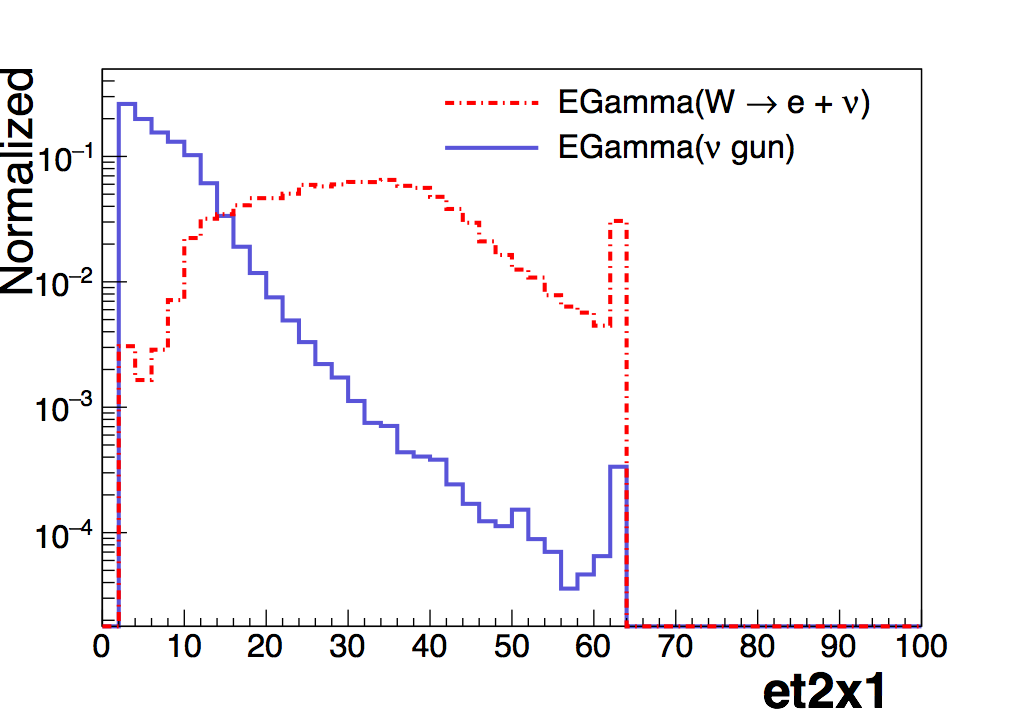
\includegraphics[width=0.5\linewidth]{figures/CMS/ECALPrimitives1.png}
    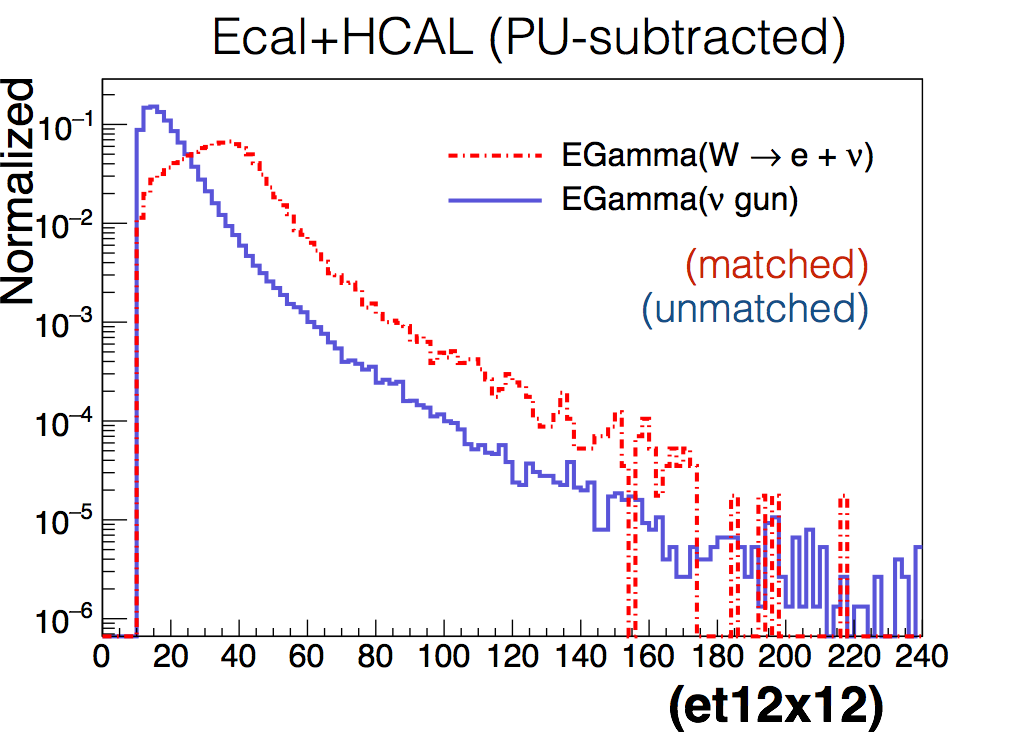
\includegraphics[width=0.5\linewidth]{figures/CMS/ECALPrimitives2.png}
  }
  }
  \makebox[\textwidth][c]{
  \subfloat[]{
  \vspace{2cm}
  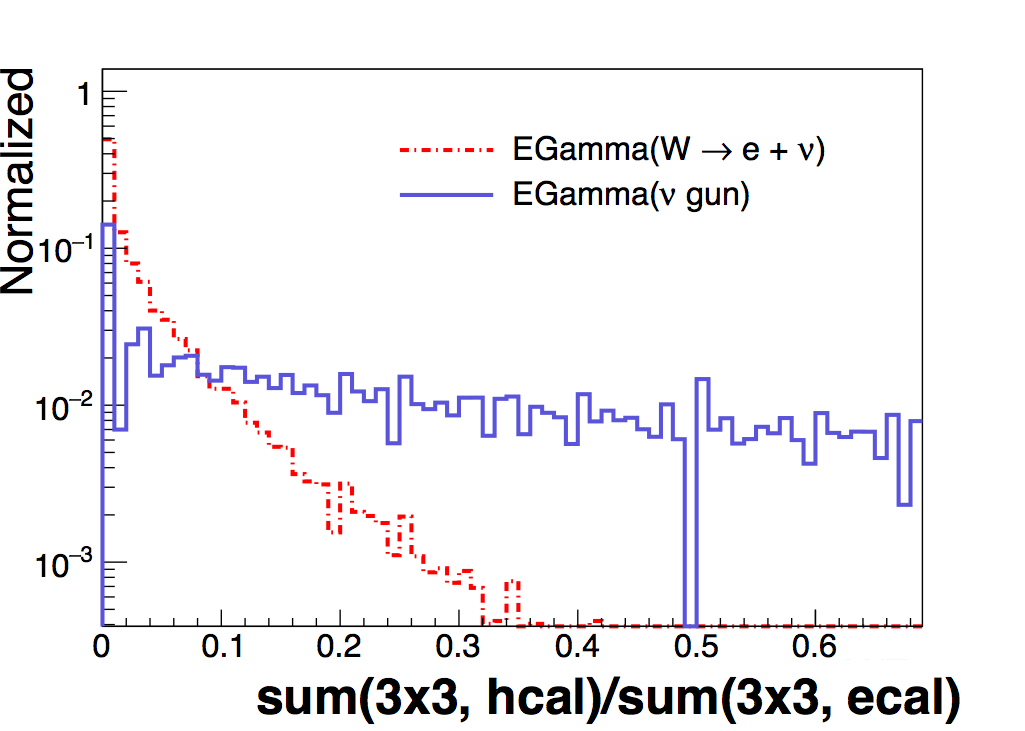
\includegraphics[width=0.5\linewidth]{figures/CMS/ECALHoE.png}
    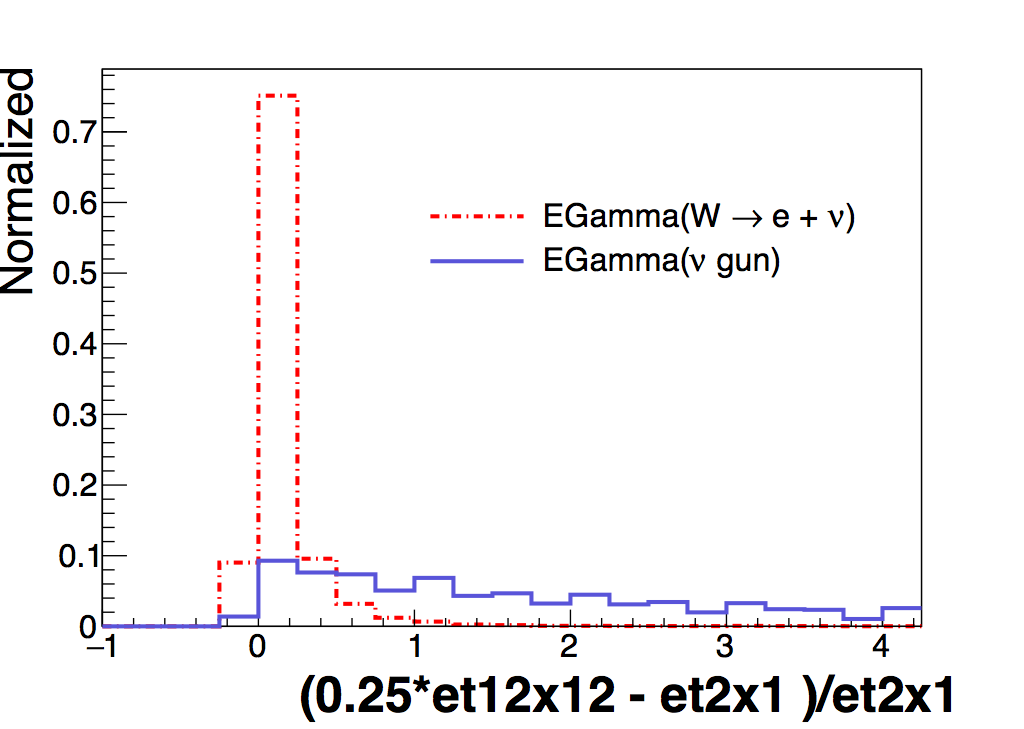
\includegraphics[width=0.5\linewidth]{figures/CMS/ECALIso.png}
}
}
\caption{The trigger primitives available from the calorimeters available to the CMS L1 trigger (a), and the observables derived from the primitives designed to discriminate between signal and background e/$\gamma$ candidates.} 
\label{fig:TriggerObservables}
\end{figure}\FloatBarrier

The efficiency, or fraction of e/$\gamma$ candidates matched to true electrons that are selected by the baseline selection of 
\begin{itemize}
\item isolation < 2.0
\item H/E < 0.5,
\end{itemize}
is shown in Fig. \ref{fig:EGammaEfficiencies} for various thresholds, shown in the figure.
\begin{figure}[h]
\makebox[\textwidth][c]{
\centering
  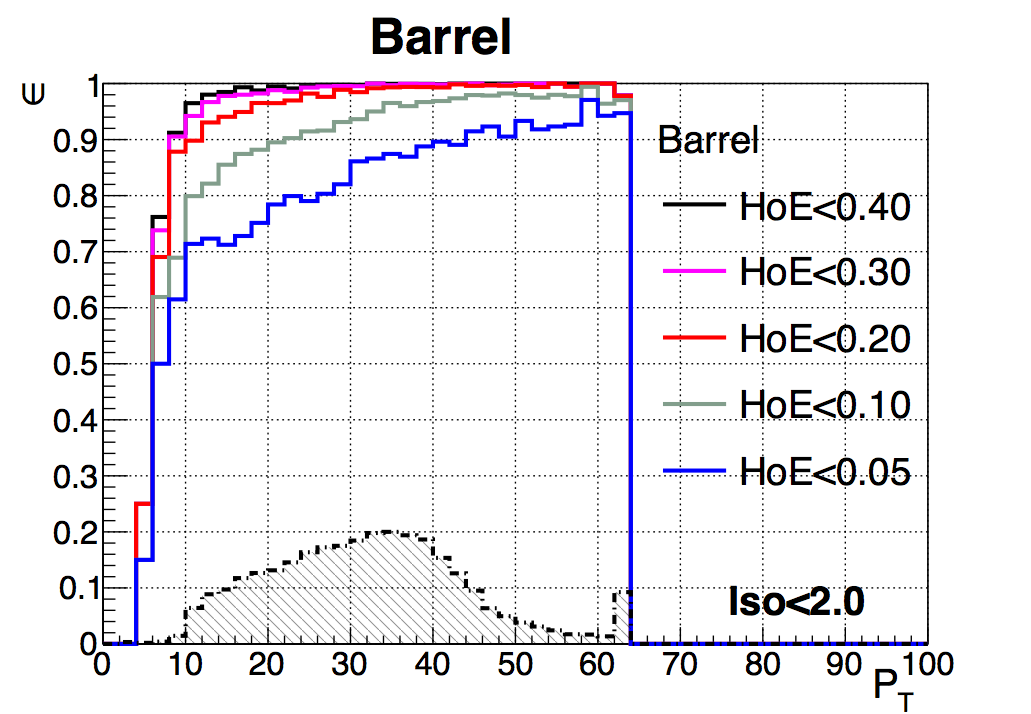
\includegraphics[width=0.49\linewidth]{figures/CMS/EcalEffIsoBarrel.png}
  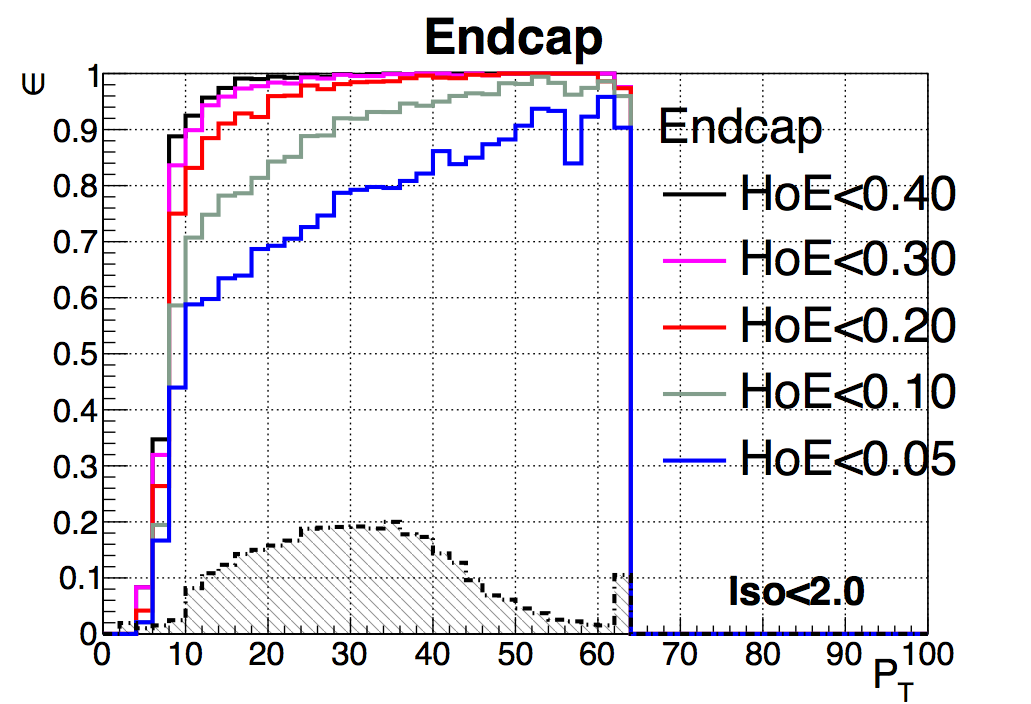
\includegraphics[width=0.49\linewidth]{figures/CMS/EcalEffIsoEndcap.png}
  }
  \makebox[\textwidth][c]{
\centering
  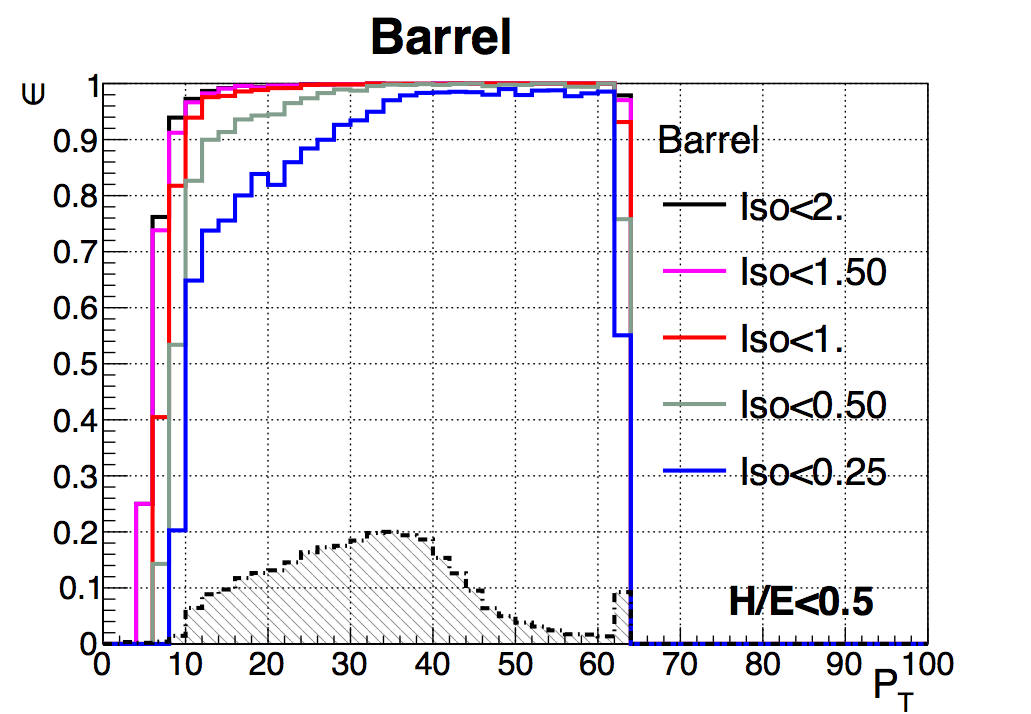
\includegraphics[width=0.49\linewidth]{figures/CMS/EcalEffHoEBarrel.png}
  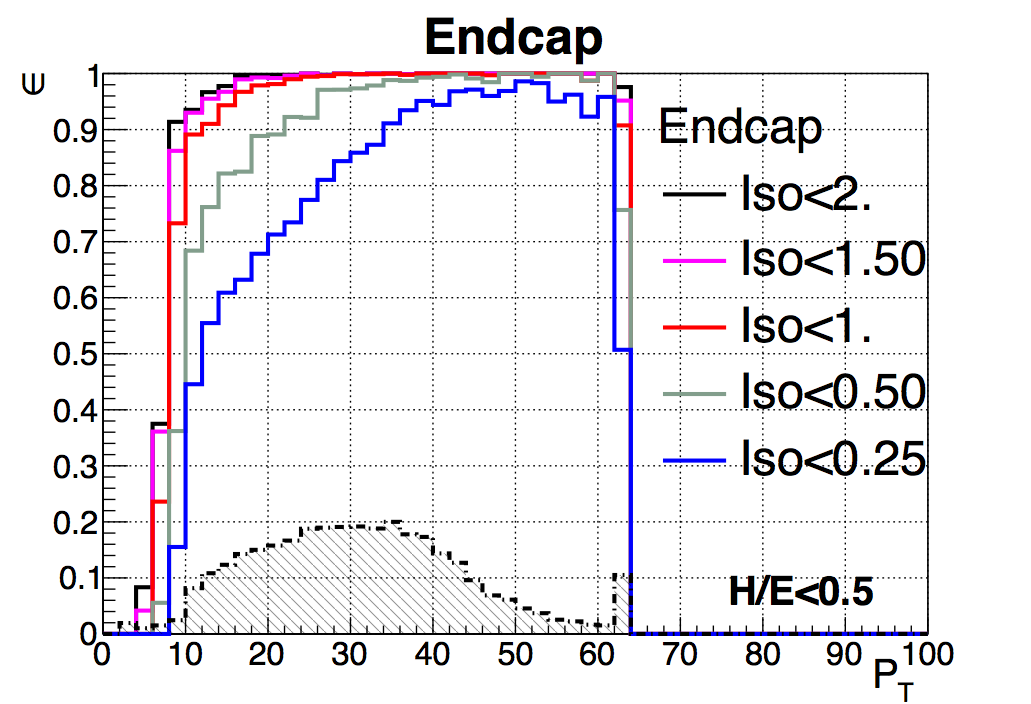
\includegraphics[width=0.49\linewidth]{figures/CMS/EcalEffHoEEndcap.png}
}
\caption{The signal efficiency in the barrel and endcap as a function of the $p_T$ of the e/$\gamma$ candidates for various thresholds on the H/E and isolation.} 
\label{fig:EGammaEfficiencies}
\end{figure}
\FloatBarrier

The performance of the currently applied cut-based selection was investigated by comparing the existing performance with that obtained through the use of an idealized discriminator. The idealized discriminator chosen was a boosted decision tree (BDT)~\cite{Hocker:2007ht} whose input variables are the observables H/E and isolation. The BDT was trained using half of the available simulated signal candidates and half of the background candidates, while half of both collections was set aside as an independent test sample. Figure \ref{fig:ECALMva1} characterizes the performance of the cut-based and BDT selection, showing the trade-off between the signal efficiency and background contamination in the test sample. The performance of the idealized discriminant is comparable to the performance of the selected working points of the cut-based approach, indicating that the values of the currently-employed selection is well-optimized. 
\begin{figure}[h]
\centering
  \includegraphics[width=0.79\linewidth]{figures/CMS/ECALMva1.png}
\caption{The background efficiency vs the signal efficiency for cut-based selection and the selection of the BDT based whose inputs are the cut-based observables. The ideal point is indicated by the gold circle located at full signal efficiency and zero background efficiency. For a given background efficiency, the cut-based signal efficiency is within a few percent of the BDT efficiency.}
\label{fig:ECALMva1}
\end{figure}

The addition of new observables in the selection was also investigated. For example, the centrality, explained in  called the centrality, explained in Fig. \ref{fig:centrality}
\begin{figure}[h]
\centering
  \includegraphics[width=0.95\linewidth]{figures/CMS/EcalCentrality.png}
\caption{The definition of the centrality (left), along with the distributions of the centrality for signal and background e/$\gamma$ candidates in simulation (right). }
\label{fig:centrality}
\end{figure}
The change in performance of the BDT with the centrality is shown in Fig. \ref{fig:ECALMva3}. Including the centrality improves the performance by about 10-15\%, which implies a 10-15\% reduction in the background rate  for a given signal efficiency. This result has been presented to the ECAL DPG working group and is available if a 10-15\% reduction in the trigger rate is required for calibrating in subsequent runs. A cut-based selection on this observable would need to be applied, since the use of multivariate discriminants is not possible, at present, in the L1 trigger.
\begin{figure}[h]
\centering
  \includegraphics[width=0.79\linewidth]{figures/CMS/ECALMva3.png}
\caption{The background efficiency vs the signal efficiency for cut-based selection, the plane BDT selection, and the selection of the BDT trained with the addition of the centrality variable. The ideal point is indicated by the gold circle located at full signal efficiency and zero background efficiency. For a given signal efficiency, a suppression of the background on the order of 10-15\% is possible. }
\label{fig:ECALMva3}
\end{figure}
\FloatBarrier


\section{Hadronic calorimeter}
Immediately surrounding the CMS ECAL and inside the CMS solenoid magnet is a sampling hadronic calorimeter (HCAL), shown in Fig. \ref{fig:HCalLayout}. Constructed from plates that alternate between steel, brass, and plastic scintillating material, the HCAL comprises a barrel with 36 azimuthal wedges covering the range $|\eta|<1.3$, and two endcaps covering the range $1.3<|\eta|<3$. The number of interaction lengths ($\lambda_{0}$) in the barrel ranges between 5 to 10 $\lambda_{0}$, and about 10 $\lambda_{0}$ in the endcaps. The geometry of the 36 barrel wedges closely matches the geometry of the 36 ECAL supermodules. An individual HCAL cell subtends the solid angle of a $5\times5$ array of ECAL crystals. The geometry of the endcaps differs from that of the ECAL.
\begin{figure}[h]
\centering
\includegraphics[width=0.95\linewidth]{figures/CMS/HCalLayout.jpg}
\caption{A schematic view of the CMS HCAL. The direction of view is toward the center of the LHC.} 
\label{fig:HCalLayout}
\end{figure}
\FloatBarrier


\section{Superconducting solenoid}
Dividing the inner detector from the outer is a 12-m long, 6-m-diameter superconducting solenoid magnet, the system most critical for the functionality of the CMS detector. Niobium Titanium coils, kept at a temperature of 3.2 K and carrying a stored energy of 2.6GJ, are responsible for filling the inner detector with a uniform 3.8 T magnetic field. The superconducting coils are cooled by liquid helium that is supplied and cooled via a multistage cryogenic system that is managed by the External Cryogenics Group of the LHC. Oil contamination in this system resulted in sub-optimal performance of the CMS solenoid in 2015, and led to a 20\textemdash30\% loss in the data collected.

 
\section{Muon system}
The outermost subdetector of CMS is the muon system. The rest of the CMS detector, 
which is nested within the muon systems, amounts to 16 interaction lengths of material, 
and so the only particles that are able to interact with the muon system are muons. Like 
the other subdetectors, the muon system coheres to the azimuthal symmetry of the CMS 
solenoid. Composed of a barrel and two endcaps, the muon system provides complete 
pseudorapidity coverage in the range $|\eta|<2.4.$ The muon detector, shown in Fig. 
\ref{fig:MuonSystem}, is made of 4 concentric, cylindrical stations, and each station is 
composed of 12 ionizing drift chambers~\cite{Breskin:1244506}. On its own, the muon system 
is capable of determining the momentum of muons with a $p_{\text{T}}$ of up to 1 TeV with 
a resolution of 15\% in the barrel and 40\% in the endcaps. When utilizing information from 
both the muon system and the inner tracker, muon momentum can generally be determined 
to within 5\%.
\begin{figure}[h]
\centering
\includegraphics[width=0.5\linewidth]{figures/CMS/MuonSystem.png}
\caption{An event display of the CMS muon system. Two muons are reconstructed in the muon system.} 
\label{fig:MuonSystem}
\end{figure}
\FloatBarrier

\section{Trigger and DAQ}
\label{sec:Trigger}

The two most critical components for the CMS detector to take data are the trigger and the data acquisition system (DAQ).  The trigger's purpose is to analyze one billion proton-proton collisions per second and quickly decide which events are to be written to disk, and which are discarded. Because of the finite computing speed and storage capacity, a maximum of about 1000 collision events per second can be recorded. Therefore, the vast majority of collisions are never reconstructed.

In order to reduce the number of events by 6 orders of magnitude, CMS employs a two-level trigger system. The two logically sequential trigger stages are: the level-1 (L1) trigger, and the high level trigger (HLT), each of which lowers the rate of events by a factor of a thousand. The L1 trigger is based on custom-manufactured programmable electronics and is responsible for analyzing each collision immediately after every bunch crossing, and discarding 99.9\% of the events. This trigger has access to coarse information from the calorimeters and muon system, namely, energy deposits in the calorimeters and hits in the muon chambers, collectively called trigger primitives. The L1 trigger uses these primitives to compute estimates of the four-vectors of $\mu$ candidates and e/$\gamma$ candidates, as well as estimates of the $\Ht$ and $\met$. The L1 trigger is allowed about 3 $\mu$s to analyze each event, and if it accepted, the event is passed to the HLT. 

The HLT, which is based in software, is capable of analyzing events with a much greater degree of sophistication than the L1. The information available to the high level trigger includes information from the CMS tracker, finely-granulated calorimetric depositions, and global objects that are constructed from the combination of all detectors.  The determination of the objects such as the $\Ht$ and $\met$ is much more precise in the HLT than in the L1, but less precise than the in the offline reconstruction.  Thus, at the analysis level, the trigger efficiency must be measured using the offline information.

The DAQ is the computer system responsible for storing information about events that have been accepted by the trigger. It is capable of processing 100 Gigabytes, or 100 events per second on average. The DAQ  integrates and analyzes the signals from about 55 million channels within the CMS detector, which are sent from about 600 independent front-end readout drivers. After processing, the DAQ sends the event information into mass storage on the CMS Tier-0 computing  enter, hosted by the CERN Data Centre.

\section{Particle and event reconstruction}
\label{sec:reconstruction}
The reconstruction of particles and event-level observables is performed by the particle flow algorithm~\cite{Beaudette:2014cea}. Particle flow analyzes the basic elements from each detector system (tracks in the tracker, calorimeter clusters, and muon tracks), and associates the elements to form single particle candidates. The final result is a global event description that attempts to characterize every particle in each event. Jets and event-level observables such as the missing transverse energy $\met$ are constructed from these particles. 

Muons are identified based on information from the muon system and the inner tracker.  Specifically, a muon is identified as a track in the muon system that is consistent in energy and direction with a track in the inner tracker. A selection is made on the $\chi^2$ of a fit of the muon track to the combined hits in the tracker and muon system, and the momentum estimated by the muon system is required to fall within three standard deviations of the estimate made by the tracker.  

Electrons are identified as tracks in the inner tracker that are spatially and energetically consistent with energy clusters in the ECAL. Because electrons can emit photons when traversing the tracker, their trajectories can exhibit abrupt changes. Therefore, a special tracking algorithm called a Gaussian Sum Filter~\cite{Beaudette:2014cea} is used to model the trajectories of electron tracks in a realistic way. The algorithm that reconstructs energy clusters in the ECAL accounts for photon emission by identifying energy deposits consistent with possible trajectories of emitted photons, and adding them to the total cluster energy.  After the track is associated with an ECAL cluster, information from the ECAL and tracker is used to identify electrons, including the quality of the fit associated with the reconstructed track,  properties related to the distribution of the energy deposited in the ECAL, the ratio of the energy deposited in the HCAL behind the relevant ECAL cluster to that deposited in the ECAL, and the individual momentum estimates from the tracker and ECAL. Charged hadrons are identified as the set of track candidates matched to ECAL clusters that did not pass the electron identification criteria. 

Photons are identified in a similar manner as electrons, but it is required that no track point in the direction of the electromagnetic energy cluster, and little or no energy deposited in the HCAL. Remaining energy deposits in the HCAL are identified as neutral hadrons. 

The result of the above algorithm is a set of particles, called particle flow candidates, representing all identified particles in the event. Jets are reconstructed by applying the anti-k$_{\text{T}}$ algorithm \cite{Cacciari:2008gp}, with a distance parameter of 0.4 or 0.5, to the particle flow candidates. Estimates of the jet energy are corrected for effects of pile-up and for non-uniformities in the detector. The jet energy resolution ranges from 5$-$20\%, depending on the jet momentum and direction. The $\met$ is computed as the magnitude of the vectorial sum of the four-momenta of all particle flow candidates and jets in the event, after the energy corrections have been applied to the jets.

\label{sec:Trigger}


\section{Phase II upgrade}
In the year 2023, the high luminosity LHC (HL-LHC) will begin operations of what is referred to as Phase II of the LHC. At that stage, the instantaneous luminosity will increase by a factor of 10 from its Run 1 design value, up to $\mathcal{L}\approx10^{35}$ cm$^{-2}$s$^{-1}$. A primary motivation for this transformation is to make it possible to study in great detail whatever phenomena may be discovered in the current phase of operation. This LHC upgrade will be accompanied by an upgrade in the hardware of the CMS detector, including improvements to various subsystems, and in some cases, the replacement of the old subsystems with new detectors. The tracker will likely be extended to cover the pseudorapidity range up to $|\eta|<4$, the muon system will likewise be extended into the forward region, the level 1 trigger system will be modified so that it considers information from the tracker in addition to the calorimeters and muon system, and the ECAL and HCAL endcaps will be replaced by more sophisticated detectors. 

Work has been carried out in preparation for the last item in this list, the calorimeter endcap upgrade. This section describes a portion of this work that I carried out. Some of the results were shown at the 2014 CMS upgrade Jamboree, and were included as part of the information that informed the decision of the down-select, in which one endcap design was selected for construction. 

\subsection{Calorimeter research and development}

Two options were considered for the set of detectors that will replace the CMS endcaps during the Phase II upgrade \cite{Bilki:2015rla}: a sampling ``shashlik'' calorimeter, and a high granularity calorimeter (HGCAL). Ultimately, the HGCAL design was chosen for construction. The shashlik calorimeter, in design, is composed of towers 114 mm in length with square cross sections of $14\times14$ mm. Each tower (Figure \ref{fig:shashtower})
\begin{figure}[h]\centering
\includegraphics[width=0.6\linewidth]{figures/CMS/Upgrade/ShashlikTower.png}\\
\caption{A shashlik calorimeter tower. }
\label{fig:shashtower}
\end{figure}
is composed of 28 layers of Tungsten alternating with 29 layers of LYSO, where LYSO (LuYSiO$_5$(Ce)) is a high density (7.1 g/cm$^3$) scintillating material largely developed for use in particle detectors by Caltech \cite{Chen:2007bb}. The HGCAL is a sampling calorimeter that will be built from alternating lead and copper sampling layers, with signal readout from silicon photosensors. The HGCAL design is notable for its ability to provide longitudinal as well as lateral information about the distribution of energy deposited by high-energy particles.

In April-May of 2014 and July-August, 2014, test beam experiments were held at Fermilab at the M-Test facility~\cite{Fermi:T1041} to study and characterize a prototype module of the shashlik calorimeter (Figure \ref{fig:shashscatter} illustrates the prototype structure). 
\begin{figure}[h]\centering
\includegraphics[width=0.6\linewidth]{figures/CMS/Upgrade/TopoMap.png}\\
\caption{A scatter plot of the accumulated track positions weighted by the in-time energy deposited in the shashlik tower, for a set of muon runs recorded in July, 2014. The $4\times4$ tower array structure, the gaps between towers, and the holes bored for the WLS fibers can be seen as green features.}
\label{fig:shashscatter}
\end{figure}
The testbeam facility provided access to beams of particles with an energy per particle ranging from 1 to 120 GeV. Several characteristics of the beam could be chosen in real time, such as the species of particles populating the beam, as well as the energy per particle.  The facility also provided the use of two wire chambers, which were used to determine the time and position of incident particles.The shashlik prototype consisted of a $4\times4$ array of towers, and each tower (Figure \ref{fig:shashtower})
\ref{fig:shashtower})
was read out by four wavelength-shifting (WLS) fibers fed longitudinally through the towers and connected to silicon photomultiplier sensors (SiPMs). 

While working help set up and manage the testbeams, I authored an interactive event display that was used to view data as it was being collected. The event display is a flexible, python-based program with a graphical user interface (GUI) that can be be used to view both live as well as stored data. The GUI is largely based on the TEve class of the Root software package \cite{Brun:1997pa}, which makes use of a slots and signals framework to enable communication between objects defined in the program. Signals carry information related to one or several user-defined objects, can be produced as a result of various actions taken by the user or from the data stream, while slots are a class of objects that are capable of receiving this information and initiating changes to their associated user-defined objects. For a concrete example, after processing the tracking information for a given event, the program produces a signal that is received by the module that projects a 3-dimensional event view, which is updated to display a set of tracks.

The event display contains several view panels, including 
\begin{itemize}
\item a heat map (color plot) of the maximum analog-to-digital count (ADC) recorded by each channel during an event in real space, as shown in Fig. \ref{fig:HeatMaps} (top);
\item a display of the readout and $\chi^2$ of the samples by channel, and a display of the pedestal noise, as shown in Fig. \ref{fig:HeatMaps}, (bottom);
\item a display of the pedestal noise by channel, where the pedestal is the expected number of ADC counts in the absence of any signal, as shown in Fig. \ref{fig:NoiseAndWires};
\item a view of the in time hits in the wire chambers, where ``in time'' refers to the criterion that the recorded time of the signal be consistent with the time of the recorded energy deposited in the calorimeter, as shown in Fig. \ref{fig:NoiseAndWires}, and
\item a 3-dimensional view of of the hits, tracks, wire chambers, and the shashlik calorimeter with color corresponding to the estimated energy deposited in each tower, as shown in Fig. \ref{fig:Shashlik3d}.
\end{itemize}
\begin{figure}[h]\centering
\includegraphics[width=0.85\linewidth]{figures/CMS/Upgrade/MuonHeatMap.pdf}\\
\vspace{-1cm}
\includegraphics[width=0.85\linewidth]{figures/CMS/Upgrade/HealthyPulses.pdf}
\caption{Top: heat maps of the ADC counts recorded at the upstream and downstream faces of the shashlik module. Bottom: Diagnostic displays of channel-by-channel information from the shashlik module. The "Chi2 Vs. Channel" display is effective at revealing noisy channels, that is, channels with a large ADC count generated by electronic noise rather than a genuine particle signal.}
\label{fig:HeatMaps}
\end{figure}
\begin{figure}[h]\centering
\includegraphics[width=0.8\linewidth]{figures/CMS/Upgrade/PedestalNoise.pdf}\\
\vspace{-1cm}
\includegraphics[width=0.8\linewidth]{figures/CMS/Upgrade/WireChambers.pdf}
\caption{Top: The pedestal noise by channel. Bottom: A scatter plot of the positions of accumulated hits and tracks recorded by the wire chambers; quality hits are colored red, and refer to hits consistent with a particle track.}
\label{fig:NoiseAndWires}
\end{figure}
\begin{figure}[h]\centering
\includegraphics[width=0.8\linewidth]{figures/CMS/Upgrade/3D_50.png}\\
\vspace{0.8cm}
\includegraphics[width=0.8\linewidth]{figures/CMS/Upgrade/3D_14.png}
\vspace{0.8cm}
\caption{Three-dimensional views of reconstructed tracks and calorimetric energy deposits in events containing a 120 GeV proton. The view can be rotated by the user, allowing different viewing perspectives of the event, as illustrated in the top and bottom figures.}
\label{fig:Shashlik3d}
\end{figure}
\noindent
The event display has since been adopted for use at testbeam experiments dedicated to studying the HGCAL, where a prototype of the future calorimeter is being characterized. The software for the event display can be obtained at the url in Ref.~\cite{bib:EventDisplay}. 

\subsubsection{Jet/\MET analysis}
After testbeam operations, I and my colleague Arka Santra performed analysis of the data collected, as well as of simulated events. The energy resolution of jets in the CMS endcaps for various phases of the CMS detector are shown in Fig. \ref{fig:ShashlikResolution}.
\begin{figure}[h]
\centering
\includegraphics[width=0.9\linewidth]{figures/CMS/Upgrade/ChsJetPerformanceEndcapTT.pdf}
\caption{The jet response (left) and energy resolution (right) in the shashlik endcap as a function of simulated jet $p_T$ in a sample of simulated $t\bar{t}$ events. The red distributions correspond to the scenario without pile-up, and pink to that with pile-up of 140 (an average of 140 collisions per bunch crossing), which is the expected amount of pile-up during the post-Phase II LHC operations. }
\label{fig:ShashlikResolution}
\end{figure}
At large $p_T$, the energy resolution in PU 140 events is seen to drop below 10\%, indicating an excellent level of performance that surpasses that described in Ref.~\cite{Bilki:2015rla}.

\FloatBarrier






%\input{inputs/Trigger.tex}
\chapter{The Viability of SUSY: The pMSSM Interpretation}
\label{chap:run1pmssm}
CMS has performed many searches for evidence of SUSY at the LHC. To assess the impact of a representative set of these searches on the MSSM, an interpretation has been performed in the framework of the phenomenological MSSM (pMSSM), taken as a proxy for the MSSM (see Section~\ref{sec:pmssm} for an introduction to the pMSSM).  A global Bayesian analysis is performed, incorporating results from a broad range of CMS searches, as well as constraints from other experiments. Because the pMSSM incorporates several well-motivated assumptions that reduce the 120 parameters of the MSSM to just 19 parameters defined at the electroweak scale, it is possible to assess the how the MSSM is constrained in a relatively straightforward way. 

This chapter begins with a brief introduction to Bayes' theorem, and follows with modified excerpts from the paper \cite{Khachatryan:2016nvf}. These sections are augmented by additional key details not discussed in the paper, including a discussion of the robustness of the results with respect to the choice of prior (prior is defined in the next section), and an expanded discussion of the non-excluded regions. But first, a short introduction to Bayes' theorem.

\section{Bayes' theorem}
Bayes' theorem, or ``the Pythagorean theorem [of] probability,'' according to eminent statistician Harold Jeffreys~\cite{Jeffreys:Inference}, is a fundamental statement in probability theory relating conditional and absolute probabilities. If A and B represent two potentially true statements, 
\begin{itemize}
\item P(A) and P(B) are the absolute probabilities of A and B being true, respectively, and
\item P(A|B) is the conditional probability of A being true given that B is true,
\end{itemize}
then Bayes' theorem is
\begin{equation}
\text{P(A|B)}=\frac{\text{P(B|A)P(A)}}{\text{P(B)}}.
\end{equation}
Bayes' theorem is applicable in many physics problems as a means of inference, namely, as a way of inferring knowledge about a theory given data:
\begin{equation}
\text{P(theory|data)}=\frac{\text{P(data|theory)P(theory)}}{\text{P(data)}}=\text{P(data|theory)P(theory)},
\end{equation}
where P(data) has been set to 1. In this expression, the factor P(theory) is called the prior probability density, and incorporates knowledge about a given theory prior to the consideration of the data at hand;  \text{P(data|theory)} is referred to as the likelihood, and incorporates the data into our knowledge about the theory; P(theory|data) is called the posterior probability density, and represents our state of knowledge about the theory given all information available. If the posterior density for a given parameter differs significantly from its prior density, then the data have provided useful information about the parameter. To make meaningful conclusions, it is necessary to start with a prior that encodes as much relevant information as possible. Bayesian inference is used in the following sections, as well as in the Chapter \ref{chap:susysearches} in the context of QCD background estimation.

\section{The pMSSM interpretation}
The purpose of this work is to assess how the current data constrain the MSSM using the more tractable pMSSM as a proxy.  The conclusions are based on the observations of a representative subset of CMS search results that analyzed data corresponding to  integrated
luminosities of 5.0 $\text{fb}^{-1}$ at 7 TeV and  19.5 $\text{fb}^{-1}$ at 8 TeV.
The considered searches include hadronic searches, both general searches and searches
targeting top squark production; also included are searches with
leptonic final states, both general and EW-targeted, as well as monojet searches. For a selected set of pMSSM parameter points, event samples were simulated using the CMS fast detector simulation \cite{fastsim} and analyzed. 
The 7 and 8 TeV data are treated consistently; in particular, the same set of points in the pMSSM model phase space are used in the analysis of all searches. This approach greatly facilitates the combination of the results from the 7 and 8 TeV (Run 1) data. The points were chosen randomly from a larger set of points that are consistent with pre-LHC experimental results and basic theoretical constraints.

The statistical analysis is based largely on the Bayesian approach of Refs. \cite{Bayes:1, Bayes:2}. The work is an extension of Ref.~\cite{Sekmen:2011cz}, which interpreted three independent CMS
analyses based on an integrated luminosity of about 1 $\text{fb}^{-1}$ of
data~\cite{Chatrchyan:2011zy,Chatrchyan:2011gqa,Chatrchyan:2012te} in
terms of the pMSSM, confirming that the approach is both feasible and
more successful in yielding general conclusions about SUSY than those based on constrained SUSY models.
Furthermore, the diversity of phenomena covered by the pMSSM is also helpful
in suggesting new approaches to searches for SUSY at the LHC. A similar study has been performed by the ATLAS experiment~\cite{Aad:2015baa}.


\section{Methods for the combination CMS analyses}
\label{sec:anl}
The results from the selected CMS analyses are used to construct posterior densities of model
parameters, masses, and observables. The posterior density of the
model parameters, which are denoted by $\theta$, is given by 
\begin{equation}
	p(\theta|D^\textrm{CMS}) \propto L(D^\textrm{CMS} | \theta\, ) \, p^\textrm{non-DCS}(\theta),
	\label{eq:posterior}
\end{equation}
where $D^\textrm{CMS}$ denotes the data analyzed by the direct CMS
SUSY searches, $L(D^\textrm{CMS} | \theta\, )$ is the associated CMS
likelihood that
incorporates the impact of these direct CMS searches, and
$p^\textrm{non-DCS}(\theta)$ is the prior density constructed from
results not based on direct CMS SUSY searches (non-DCS results).
The posterior density for a single observable $\lambda$ is obtained by integrating the full posterior density over the parameters,
\begin{equation}
	p(\lambda|D^\textrm{CMS}) = \int \delta[\lambda- \lambda^\prime(\theta)] \, p(\theta| D^\textrm{CMS}) \, d\theta,
	\label{eq:lambda}
\end{equation}
where $\lambda^\prime(\theta)$ is the value of the observable as
predicted by model point $\theta$ ($\theta$ identifies the model point). Equation~\ref{eq:lambda} is approximated using Monte Carlo (MC) integration.  

\subsection{Construction of the prior}
\label{sec:prior}
The prior $p^\textrm{non-DCS}(\theta)$
encodes the boundaries of the considered parameter space, the constraints from non-DCS data, and several theoretical conditions. It is formulated as a product of four factors,
\begin{align}
	p^\textrm{non-DCS}(\theta) &\propto \left [ \prod_j L(D_j^\textrm{non-DCS} | \lambda_j(\theta)) \right] \,
		\cdot p(c\tau(\tilde{\chi}^\pm) < \textrm{10 mm}|\,\theta\,) \,
		 \cdot p(\textrm{theory}|\theta\,) \,
		 \cdot p_0(\theta),
		\label{eq:prior}
\end{align}
which I will explain one by one.

The initial prior $p_0(\theta)$ is taken to be uniform in the pMSSM sub-space (see Section \ref{sec:pmssm} for definitions of the parameters),
\begin{eqnarray}
	&-3 \le M_1, M_2 \le 3 ~ TeV,& \nonumber\\
	&0 \le M_3 \le 3 ~ TeV,			& \nonumber\\
	&-3 \le \mu \le 3 ~ TeV,		& \nonumber\\
	&0 \le m_{\rm A} \le 3 ~ TeV,			& \nonumber\\
	&2 \le \tan\beta \le 60,		& \nonumber\\
	&0 \le m_{{\tilde{\text{Q}}_{1,2}}}, m_{{\tilde{\text{U}}_{1,2}}}, m_{{\tilde{\text{D}}_{1,2}}}, m_{{\tilde{\text{L}}_{1,2}}}, m_{{\tilde{\text{E}}_{1,2}}}, m_{{\tilde{\text{Q}}_3}}, m_{{\tilde{\text{U}}_3}}, m_{{\tilde{\text{D}}_3}},m_{{\tilde{\text{L}}_3}}, m_{{\tilde{\text{E}}_3}} \le 3 ~ TeV,	& \nonumber\\
	&-7 \le A_{\text{t}}, A_{\text{b}}, A_\tau \le 7 ~ TeV,
\label{eq:subspace}
\end{eqnarray}
and the formally unbounded 
SM subspace defined by $m_{\rm t}$, $m_{\rm b}(m_{\rm
  b})$, and $\alpha_{\rm s}(m_{\rm Z})$; the non-DCS measurements, which are listed in Table~\ref{tab:preCMS}, constrain these SM parameters to narrow ranges.   
The sub-space defined in Eqs. (\ref{eq:subspace}) 
covers the 
phenomenologically viable parameter space for the LHC and 
is large enough to cover sparticle masses to which the LHC might
conceivably be 
ultimately sensitive.  
The term $p(\textrm{theory} |\,\theta\,)$  imposes the theoretical constraints listed at the end of Section~\ref{sec:pmssm}. In this study, signal events were simulated using a fast detector simulation program~\cite{fastsim} that does not accurately model the detector response to massive long-lived charged particles traversing the calorimeters. Therefore, the parameter space considered has been restricted to the set of model points for which the chargino decays quickly, having a mean lifetime of $c\tau(\tilde{\chi}^\pm)<10\text{ mm }$.  The factor $p(c\tau(\tilde{\chi}^\pm)<10\text{ mm } |\, \theta\,)$ imposes this requirement. Both  $p(\textrm{theory} |\, \theta\,)$ 
and $p(c\tau(\tilde{\chi}^\pm)<10\text{ mm } |\,\theta\,)$ are unity if the
inequalities are satisfied and zero otherwise. 


The product of likelihoods $L(D^\mpreCMS|\lambda(\theta))$ in
Equation (\ref{eq:prior}) over measurements $j$ is associated with \preCMS~ data, $D^\mpreCMS$,
which imposes constraints from precision measurements and a selection
of pre-LHC searches for new physics. The measurements used and their associated likelihoods are listed in Table~\ref{tab:preCMS}.
Data from DM experiments has not been included in the prior in order to avoid bias from cosmological assumptions (e.g., DM density and distribution, assumption of one thermal relic, no late entropy production, etc.).
%\subsubsection{Sampling of prior}

Since the explicit functional dependence of the prior $p^\textrm{\preCMS}(\theta)$ on
$\theta$ is not available \emph{a priori}, but the predictions $\lambda(\theta)$ are available point by point, it is natural to represent the prior as a set of points sampled from it.  Owing to the complexity of the parameter space, the sampling is performed
using a Markov chain Monte Carlo (MCMC) 
method~\cite{MCMC1,MCMC2,MCMC3,MCMC4,Bayes:2}. 


% The \preCMS data included in the prior are shown in
% Table~\ref{tab:preCMS}.  All data except Higgs signal strenths $\mu_h$
% were used in the original MCMC scan.  However, measurements marked
% "reweight" in the last column were updated during this study, and the
% scanned points were reweighted to take into account the updated
% effects, as described in Appendix~\ref{sec:mcmcorigvars}, along with
% the original measurement values.


All data in Table~\ref{tab:preCMS} except the Higgs boson signal strengths $\mu_{\rm h}=\sigma/\sigma_{\text{SM}}$ were used in the
original MCMC scan. The $\mu_{\rm h}$ measurements were incorporated into the prior post-MCMC.    
A number of measurements, marked ``reweight'' in the last column, were updated during the course of this study as new results
became available.  The weights, applied to the subset of scan points which were selected for simulation, were computed as the ratio of the likelihoods of the new measurements shown in
Table~\ref{tab:preCMS} to the previous measurements.    
%the original ones used in the MCMC sampling and the reweighting procedure are detailed in Appendix~\ref{sec:mcmcorigvars}. 

\begin{table}[htb]
\caption{The measurements that are the basis of the \preCMS prior
  $p^\mpreCMS(\theta)$ for the pMSSM parameters, their observed values and likelihoods. The observables are the decay branching fractions ${\cal B}({\rm b} \rightarrow
  {\rm s}\gamma)$ and ${\cal B}({\rm B}_{\rm s} \rightarrow \mu \mu)$,
  the SUSY to SM ratio for the
  branching fraction of the decay B$^{\rm +}\rightarrow \tau \nu$ (R$[$B$^{\rm +}\rightarrow \tau \nu])$,
  the difference in the muon anomolous magnetic moment from its SM
  prediction $\Delta a_\mu$, the strong coupling constant
  at the Z boson mass $\alpha_{\rm s}(m_{\rm Z})$,  the top and bottom quark masses
  $m_{\rm t}$ and $m_{\rm b}(m_{\rm b})$, the Higgs boson mass $m_{\rm h}$ and signal strength $\mu_{\rm h}$, and sparticle mass limits from LEP.  All data except $\mu_{\rm h}$ were used in the initial MCMC scan. See text for details.}
\vspace{1ex}
%\resizebox{\textwidth}{!}{
\begin{center}
\begin{tabular}{c|r|r|r|r}
\hline
$i$     & Observable    & Constraint   & Likelihood function & Comment \\
        & $\mu_i(\theta)$  & $D^\mpreCMS_i$  &  $L[D^\mpreCMS_i|\mu_i(\theta)]$ & \\
\hline\hline
1 & ${\cal B}({\rm b} \rightarrow {\rm s}\gamma)$~\cite{Amhis:2014hma} & $(3.43 \pm 0.21^{\rm
  stat} \pm 0.24^{\rm th} \pm 0.07^{\rm sys})\times 10^{\rm -4}$ & Gaussian & reweight \\
\hline
2 & ${\cal B}({\rm B}_{\rm s} \rightarrow \mu \mu)$~\cite{CMS:2014xfa} & $(2.9 \pm
0.7 \pm 0.29^{\rm th})\times 10^{-9}$ & Gaussian & reweight \\
\hline
3 & R(B$^{\rm +}\rightarrow \tau \nu$)\cite{Amhis:2014hma} & $1.04\pm 0.34$ & Gaussian & reweight \\
\hline
4 & $\Delta a_\mu$~\cite{Hagiwara:2011af} & $(26.1 \pm 6.3^{\rm
  exp}\pm 4.9^{\rm SM} \pm 10.0^{\rm SUSY})\times 10^{\rm -10}$ & Gaussian & \\
\hline
5 & $\alpha_{\rm s}(m_{\rm Z})$~\cite{Agashe:2014kda} & $0.1184 \pm 0.0007$ & Gaussian & \\
\hline
6 & $m_{\rm t}$~\cite{CDF:2013jga} & $173.20\pm0.87^{\rm stat}\pm1.3^{\rm sys}$~GeV & Gaussian & reweight \\
\hline
7 & $m_{\rm b}(m_{\rm b})$~\cite{Agashe:2014kda} & $4.19^{\rm +0.18}_{\rm -0.06}$~GeV & Two-sided Gaussian & \\
\hline
\multirow{2}{*}{8} & \multirow{2}{*}{$m_{\rm h}$} & \multirow{2}{*}{LHC: $m_{\rm h}^{\rm low} = 120$\GeV, $m_{\rm h}^{\rm high} = 130$\GeV }& 1 if
$m_{\rm h}^{\rm low} \le m_{\rm h} \le m_{\rm h}^{\rm high}$ & \multirow{2}{*}{reweight} \T\B\\
   &             &                               & 0 if $m_{\rm h} <
   m_{\rm h}^{\rm low}$ or $m_{\rm h} > m_{\rm h}^{\rm high}$ & \B\\
\hline
9 & $\mu_{\rm h}$ & CMS and ATLAS in LHC Run 1, Tevatron & {\sc Lilith} 1.01~\cite{Bernon:2014vta,Bernon:2015hsa} & post-MCMC \\
\hline
\multirow{2}{*}{10} & Sparticle & LEP \cite{lepsusy} & 1 if allowed & \\
   & masses & (via {\sc micrOmega}~\cite{Belanger:2001fz,Belanger:2004yn,Belanger:2008sj}) & 0 if excluded &  \\
\hline
\end{tabular}
%}
\end{center}
\label{tab:preCMS}
\end{table}


For a given point $\theta$, the predictions $\lambda(\theta)$ --- including those needed
to calculate the likelihoods $L(D^\mpreCMS|\lambda(\theta))$ --- are obtained as follows. 
The physical masses and interactions are calculated 
using the SUSY spectrum generator {\sc SoftSUSY} 3.3.1~\cite{Allanach:2001kg},
with the input parameters $\theta$ defined at $M_{\rm SUSY}=\sqrt{m_{\tilde{\text{t}}_{1}}m_{\tilde{\text{t}}_{2}}}$. 
This calculation includes 1-loop corrections for sparticle masses and mixings, 
as well as 2-loop corrections for the small Higgs boson mass.
Low-energy constraints are calculated with {\sc SuperIso}
v3.3~\cite{Mahmoudi:2008tp}. {\sc micrOMEGAs} 2.4.5~\cite{Belanger:2001fz,Belanger:2004yn,Belanger:2008sj} is used 
to check the compatibility of pMSSM points with sparticle mass limits from LEP and other pre-LHC experiments. {\sc micrOMEGAs} is also used to compute the DM relic density, and the spin-dependent and spin-independent DM-nucleon scattering cross sections; these observables are not used in the construction of the prior, but it is shown how they are affected by the CMS searches. The program  {\sc SDECAY} 1.3~\cite{Muhlleitner:2003vg} is used to generate sparticle decay tables and 
{\sc HDECAY} 5.11~\cite{Djouadi:1997yw} to generate Higgs boson decay tables.
The program {\sc Lilith} 1.01~\cite{Bernon:2014vta,Bernon:2015hsa} is used for evaluating the Higgs boson signal likelihood based on ATLAS~\cite{ATLAS-CONF-2014-009}
and CMS~\cite{Khachatryan:2014jba} measurements, following the approach
explained in Section~2.3 of Ref.~\cite{Dumont:2013npa}. The experimental results used in {\sc Lilith} are the signal strengths
of the Higgs boson decay modes $Y=(\gamma\gamma,\,{\rm WW}^*,\,{\rm ZZ}^*,{\rm
  b}\bar {\rm b},\tau\bar{\tau})$ in terms of the primary Higgs boson production modes
gluon-gluon fusion (ggF), vector boson fusion (VBF), associated
production with a W or Z boson (Wh and Zh, commonly denoted as
Vh), and associated production with a top-quark pair (t$\bar{\text{t}}$h) as
published by ATLAS, CMS,
and Tevatron experiments.
When these signal strengths are given as 2-dimensional (2D) confidence level (CL) contours in, e.g., the
$\mu_{\rm ggF+tth}(Y)$ versus $\mu_{\rm VBF+Vh}(Y)$ plane, the
likelihood is approximated by fitting a 2D Gaussian function to the 68\%~CL
contour provided by the experiments.
For each experiment, a $\chi^2$ is computed using $- 2 \log L_Y
= \chi_Y^2$ for each decay mode $Y$, and the combined $\chi^2$ is
then obtained by summing over all the individual $\chi_Y^2$ values.
Additional information on signal strengths (and invisible decays) in
one dimension is included analogously, using the published likelihood function
when available or else the Gaussian approximation.
 
The uncertainty in the anomalous magnetic moment of the muon includes a component that accounts for theoretical uncertainties in the SUSY calculations.

The large window on the Higgs boson mass of 120--130 GeV covers the theoretical uncertainty in the Higgs boson
mass calculation in the MSSM. All tools use the SUSY Les Houches accord~\cite{Skands:2003cj} for
data entry and output.  Approximately 20 million points are sampled from $p^\textrm{non-DCS}(\theta)$ using multiple MCMC chains, but omitting the prompt chargino requirement. When that requirement is imposed, the number of sampled points is reduced by 30\%, and the fraction of bino-like LSPs (see Chapter \ref{chap:susy} Section \ref{sec:mssm}) is enhanced from about 40 to 50\%. A random subsample of 7200 points is selected for simulation studies. Given the large dimensionality of the model, this is a rather sparse scan. Nevertheless, the scan density is sufficient to learn much about the viability of the pMSSM model space. Distributions of model parameters in this subsample were compared with distributions from independent subsamples of similar size, as well as distributions from the original large sample, and consistency between distributions was observed within statistical uncertainties. 




\subsection{Incorporation of the CMS data}
\label{sec:cmslhd}
The analyses considered in this work are those listed in Table~\ref{tab:CMS}, and explore final-states 
characterized by a variety of event-level observables:
the scalar sum of the transverse momenta of jets (\HT{}); the magnitude of the vector sum of 
the transverse momenta of final-state particles (\MET{} or \MHT{}); a measure of the transverse
mass~\cite{Lester:1999tx} (see Appendix \ref{app:discriminators} for more details) in events in which two particles each decay to one invisible and one reconstructed particle (\MTtwo{}); the multiplicity of jets identified as originating from a b quark (b-jets); and a
range of lepton multiplicities, including opposite-sign (OS) and
like-sign (LS) lepton pairs.  Other analyses that were not included in this study but which may impose additional constraints on the model space include  searches for SUSY in the single lepton channel with one or multiple b-jets~\cite{Chatrchyan:2013iqa} and searches for top squark production~\cite{Chatrchyan:2013xna} in the single lepton channel. The searches considered comprise hundreds of signal regions and address a large diversity of possible signal topologies.

\begin{table}[htb]
\caption{The CMS analyses considered in this study.  Each row gives the analysis description, the center-of-mass energy at which data were collected,
  the associated integrated luminosity,
  the likelihood used,
  and the reference to the analysis documentation.
  %Except where indicated otherwise, all analysis channels are taken into account.
  }
\begin{center}
\begin{tabular}{l|l|l|l}
\hline
\multicolumn{1}{c|}{Analysis} & \multicolumn{1}{|c|}{$\sqrt{s}$ [TeV]} & \multicolumn{1}{|c|}{$\mathcal{L}$ [fb$^{-1}$]} & \multicolumn{1}{|c}{Likelihood} \\
\hline
Hadronic \HT{} + \MHT{} search \cite{SUS12011} & 7  & 4.98 & counts \\
Hadronic \HT{} + \MET{} + b-jets search  \cite{SUS12003} & 7  & 4.98 & counts\\
Leptonic search for EW prod. of $\widetilde{\chi}^0$,
$\widetilde{\chi}^{\pm}$, $\tilde{\rm l}$ \cite{SUS12006} & 7  & 4.98 & counts \\
\hline
Hadronic \HT{} + \MHT{} search \cite{SUS13012} & 8  & 19.5 & counts\\
Hadronic \MTtwo{} search \cite{Chatrchyan:2012jx} & 8 & 19.5 & counts\\
%expected: $\alpha_\mathrm{T}$ search &?&?&?&\\
Hadronic \HT{} + \MET{} + b-jets search \cite{SUS12024} & 8 & 19.4 & $\chi^2$\\
Monojet searches \cite{Khachatryan:2014rra} & 8  & 19.7 & binary\\
Hadronic third generation squark search \cite{Khachatryan:2015wza}  & 8 & 19.4 & counts\\
%expected: razor+b search &?&?&?&\\
OS dilepton (OS ll) search \cite{Khachatryan:2015lwa} & 8 & 19.4 & counts\\
(counting experiment only) & & & \\
LS dilepton (LS ll) search \cite{SUS13013} & 8 & 19.5 & counts\\
(only channels w/o third lepton veto)& & & \\
Leptonic search for EW prod. of $\widetilde\chi^0$,
$\widetilde{\chi}^{\pm}$, $\tilde{\rm l}$ \cite{SUS13006} & 8 & 19.5 & counts\\
(only LS, 3 lepton, and 4 lepton channels)& & &\\
\hline
Combination of 7 TeV searches & 7 & - & binary  \\
Combination of 7 and 8 TeV searches & 7,8 & - & binary  \\
\hline
\end{tabular}
\label{tab:CMS}
\end{center}
\end{table}
 

The CMS likelihoods $L(D^\mCMS|\,\theta)$ are calculated for each of these analyses (or combinations of analyses), using different forms of likelihood depending on the nature of the results that are available.
The first form of likelihood (\emph{counts}) uses observed counts,
$N$, and associated background estimates, $B \pm \delta B$; the second
($\chi^2$) uses profile likelihoods (Section \ref{sec:freqcheck} gives a discussion on profile likelihoods), 
$T(\mu, \theta)$, where $\mu =
\sigma / \sigma^\textrm{SUSY}(\theta)$ is the signal strength modifier
and $\sigma$ and $\sigma^\textrm{SUSY}(\theta)$ are the observed and
predicted SUSY cross sections, respectively, while the third
(\emph{binary}) joins either of the first two kinds of result together
with a signal significance measure $Z$, and is used for combining
results from overlapping search regions. The three forms of the
likelihood used and the signal significance measure $Z$ are described in the following.

%Details of these likelihoods and the signal significance measure are given in Appendix~\ref{sec:likelihoods}.

\textbf{Counts likelihood}
For a single-count analysis, the likelihood is given by  
\begin{equation}
L(D^\mCMS|\theta\,) = \int \textrm{Poisson}(N | s(\theta) + b) \, p(b|B, \delta B) db,
\label{eq:lhd_counts}
\end{equation}
where $N$ is the observed count,
$s(\theta)$ and $b$ are the expected number of signal and background counts, respectively,
and $B \pm\delta B$ is the estimated number of background event counts and its uncertainty.
The prior density for $b$, $p(b|B, \delta B)$, is modeled as a gamma density, 
$\textrm{gamma}(x;\alpha,\beta) = \beta \exp(-\beta x)  (\beta x)^{\alpha-1}/\Gamma(\alpha)$,
with $\alpha$ and $\beta$ defined such that the mode and variance of the gamma density are  $B$ and $(\delta B)^2$, respectively. 
%This likelihood provides an accurate description of statistical uncertainties and
%describes systematic uncertainties in an approximative way.
For analyses that yield multiple independent counts, the likelihood is
the product of the likelihoods of the individual counts. For analyses
with multiple counts, the background predictions for the different search regions are treated as uncorrelated.  Systematic effects on the signal counts are taken into account by varying the signal yield by multiplying it with a signal strength modifier $\mu$ with values $1-\delta\mu, 1, 1+\delta\mu$, where $\delta\mu$ is the fractional value of the systematic uncertainty.

\textbf{$\chi^2$ likelihood}
This likelihood is used for CMS searches that provide profile
likelihoods, $T(\mu,\theta) \equiv
L(D^\mCMS|\mu,\theta,\hat\nu(\mu,\theta))$, for the signal strength
modifier $\mu$, where $\nu$ represents the nuisance parameters and
$\hat\nu(\mu,\theta)$ their conditional maximum likelihood
estimates. Taking $\hat\mu$ to be the signal strength modifier that
maximizes $T(\mu,\theta)$, it can be shown that the quantity $t =
-2\ln\left[T(1,\theta)/T(\hat\mu,\theta)\right]$ follows a $\chi^2$
density with one degree of freedom in the
asymptotic limit~\cite{Wilks:1938dza},
\begin{eqnarray}
L(D^\mCMS|\theta\,) & \approx &\exp(-t/2) / \sqrt{2\pi t}, 
  ~\label{eq:lhd_chi2}
\end{eqnarray}
which is adopted as the CMS likelihood in this case. The systematic uncertainties in the signal yield can again be incorporated by varying the values of $\mu$.
%This likelihood provides a good description of systematic and statistical uncertainties.

\textbf{$Z$-significance}
This study uses a signal significance measure defined by 
\begin{align}
  Z(\theta) = \textrm{sign} [\ln B_{10}(D, \theta )] \sqrt{2 | \ln B_{10}(D, \theta )|} ,
  \label{eq:Zsingle}
\end{align}
where 
\begin{equation}
  B_{10}(D, \theta) = \frac{L(D | \theta, H_1)}{L(D | H_0)} 
  \label{eq:B10}
\end{equation}
is the local Bayes factor for data $D$, at point $\theta$, and $L(D | \theta, H_1)$ and $L(D  | H_0)$
are the likelihoods for the signal plus background ($H_1$) and background only ($H_0$) hypotheses, respectively.  The function $Z(\theta)$ is a signed Bayesian analog of the frequentist ``$n$-sigma".
The case $Z \gg 0$ would indicate the presence of a signal 
at a significance of $Z$ standard deviations, while the case $Z \ll 0$ would indicate the absence of signal, i.e., an \emph{exclusion} at a significance of $Z$ standard deviations.  The $Z$-significance is the basis of the binary likelihood.

\textbf{Binary likelihood}
This likelihood is used for combining results from search regions in
which data may not be independent, for example, multiple counts from
overlapping search regions.  The data are first divided into subsets for
which either a count or $\chi^2$ likelihood can be calculated.  For
each subset $j$, with data $D_j$, $Z_j(\theta)$ is computed using Equation 
(\ref{eq:Zsingle}).  An overall significance measure that includes all subsets under consideration is defined by
\begin{equation}
  Z(\theta) \equiv  Z_{j_{\rm max}}(\theta),
  \label{eq:Zmulti}
\end{equation}
where $j_{\rm max}$ is the index of the maximum element in the set \{$|Z_j(\theta)|$\}.
This quantity is used to define the binary likelihood as follows,
\begin{equation}
  L(D^\mCMS|\theta\,) =
  \begin{cases}
    1 & \text{if } Z(\theta) > -1.64, \\
    0 & \text{if } Z(\theta) \leq -1.64,
  \end{cases}
  \label{eq:lhd_binary}
\end{equation}
where $Z(\theta)=-1.64$ corresponds to the frequentist threshold for
exclusion at the 95\% CL. Systematic uncertainties are incorporated by computing each $Z_j(\theta)$ with varying  values of $\mu$, and using these recalculated $Z_j(\theta)$ to compute the binary likelihood.  
Although use of the binary likelihood entails a loss of information, it is a convenient approach in cases of non-disjoint data, where a proper likelihood calculation is not feasible without more information.  In this study, binary likelihoods are used for the monojet searches, which have overlapping search regions, and for combining the 7 TeV, and 7$+$8 TeV results, where the analyses use non-disjoint data.

To compute likelihoods and $Z$-significances,  expected signal counts for
the search regions of each analysis are computed
for the 7200 pMSSM points. The simulated events for each model point, which were generated using {\sc pythia} 6.4~\cite{Sjostrand:2006za} and processed with the CMS fast detector simulation program~\cite{Abdullin:2011zz}, are passed through the analysis procedures in order to determine the counts.  For each pMSSM point, 10,000 events have been simulated.  

%%%%%%%%%%%%%%%%%%
% gluino mass
%%%%%%%%%%%%%%%%%%
\section{Results}
\label{sec:results}

The results of the study are presented in terms of three types of comparisons. The first type of comparison is of the distribution of the $Z$-significance for different combinations of analyses.
The second comparison is between the prior and posterior densities of the pMSSM parameters.
The third comparison is between the total number of points in the pMSSM parameter space, and the number of points that survive the CMS analyses considered. For the last comparison, the survival probability is shown as a function of model parameters, where the survival probability in a region $\Theta$ of the pMSSM parameter space, is defined by
\begin{equation}
  \frac{\int_\Theta p^\textrm{non-DCS}(\theta)H(Z(\theta) + 1.64)d\theta}{\int_\Theta p^\textrm{non-DCS}(\theta) \, d\theta},
  \label{eq:Survive}
\end{equation}
where $H$ is the Heaviside step function with a threshold value $Z = -1.64$, which
again is the threshold for exclusion at the 95\% CL. 

%%%%%%%%%%%%%%%%%%
% Z
%%%%%%%%%%%%%%%%%%
\subsection{Global significance}
Distributions of $Z$-significance are shown in Fig. \ref{fig:Z} for all the CMS
searches included in this study: 8 TeV searches, combinations of 7 TeV searches, and combinations of
7$+$8 TeV searches. The farther a $Z$ distribution is from zero, the
greater the impact of the analysis on the pMSSM parameter space.   As
noted in Section \ref{sec:anl}, negative and positive values indicate a preference for the background only ($H_0$) and the signal plus background ($H_1$) hypotheses, respectively.

All 8 TeV searches lead to distributions with negative tails,
indicating that each disfavors some region of the pMSSM parameter space.
The searches making the greatest impact are the \HT{}$+$\MHT{} and \MTtwo{}
searches, which disfavor a significant portion of the parameter space.
The \MTtwo{}, \HT{}$+$\MET{}$+$b-jets, EW, and OS dilepton searches,
which yield modest excesses over the SM predictions, have
$Z$-significances up to 4.

As expected, the combined 7$+$8 TeV result has a greater impact than any individual analysis. 
Overall, the impact of the 7 TeV combined result is relatively small as indicated by the high peak around zero. 


\begin{figure}[t]
\centering
\resizebox{0.8\linewidth}{!}{
  \begin{tabular}{c}
  \incfigNum{(a)}{inclusive.pdf}
  \incfigNum{(b)}{hadExcl.pdf} \\
  \incfigNum{(c)}{leptonic.pdf} 
  \incfigNum{(d)}{combined.pdf}
  \end{tabular}
}
\vspace{1mm}
\caption{The distribution of model points, weighted by the \preCMS~ prior density, of the $Z$-significance for the individual 8 TeV searches (a--c), and for 7 TeV combined and 7$+$8 TeV combined searches (d). The leftmost bins contain the underflow entries.}
\label{fig:Z}
\end{figure}
\FloatBarrier
%%%%%%%%%%%%%%%%%%
% gluino mass
%%%%%%%%%%%%%%%%%%
\subsection{Impact on parameters}
Figure \ref{fig:mg} shows the impact of the CMS searches on our
knowledge of the gluino mass. Figures \ref{fig:mg} (a)-(d) show marginalized
distributions of the gluino mass.  Posterior distributions obtained
using three  signal strength modifier values $\mu = 0.5, 1.0, 1.5$
illustrate the effect of a $\pm50$\% systematic uncertainty in the
predicted SUSY signal yields.  Since the uncertainty in the signal efficiency typically varies between 10 and 25\%, and the uncertainty in the signal cross section ranges between 30 and 50\%, this prescription is considered to be conservative. Figure \ref{fig:mg} (a) shows the strong impact of
the hadronic analyses on the gluino mass distribution.  The
\HT{}$+$\MHT{} search strongly disfavors the region below 1200~\GeV,
while the \MTtwo{} search leads to a distribution with two regions of peaking probability, one at relatively low mass, around 600 to 1000~\GeV, and one
above 1200~\GeV.  In Fig. \ref{fig:mg} (b), the other hadronic
analyses also disfavor the low-mass region, though to a lesser degree,
 and two of these analyses (the \HT{}$+$\MET{}$+b$-jets and the
 hadronic third generation) also exhibit secondary
 preferred regions around 1100~\GeV, while Fig. \ref{fig:mg} (c) shows that the EW, OS dilepton, and LS dilepton searches have little impact on the gluino mass distribution.
Figure \ref{fig:mg} (d) compares the  prior distribution to posterior distributions after inclusion of the combined 7 TeV and combined 7$+$8 TeV data.  The 7 TeV data already have sufficient sensitivity to exclude much of the low-mass gluino model space, and the 8 TeV data further strengthen this result. The enhancements induced by the hadronic
searches in the 800\textendash1300~\GeV~ range disappear in the combination
since the observed excesses driving the enhancements are not
consistent with a single model point or group of model points.


\begin{figure}[t]
    \sixpackNum{mg}
\vspace{1mm}
    \caption{\captionOneD{gluino mass}{gluino mass}}
    \label{fig:mg}
\end{figure}

Figure \ref{fig:mg} (e) shows the survival probability (Equation \ref{eq:Survive}) as a function of gluino mass
for the combined 7~ TeV, and 7$+$8 TeV results. 
The CMS searches exclude all the pMSSM points with a gluino mass below 500~\GeV, and can probe scenarios up to the highest masses covered in the scan.  As may be expected, masses of order 3 TeV are not probed directly but rather through the production of lighter particles in the model.   
Finally, Fig. \ref{fig:mg} (f) shows the $Z$-significance versus gluino mass.  A
slight negative correlation for positive $Z$ values and gluino masses
is observed below 1200~\GeV; $Z$ declines slightly as mass
increases, which indicates that some small excesses of events observed by the various searches are consistent with models with light gluinos.  

%%%%%%%%%%%%%%%%%%
% squark LCSP mass
%%%%%%%%%%%%%%%%%%

Figures \ref{fig:mq} and~\ref{fig:mLCSP} similarly summarize the impact
of searches on the first- and second-generation left-handed up squark mass and the mass of the lightest colored SUSY particle (LCSP), respectively.  The picture is similar to that for the gluino mass.  For both $\suL$ and the LCSP, the \MTtwo{} search shows a preference for masses from 500 to 1100~\GeV.  The overall impact of the searches on $\suL$ is less than the impact on the gluino mass owing to the more diverse gluino decay structure that can be accessed by a greater number of searches.  For the LCSP, the overall impact is the least  because the LCSP has the fewest decay channels; nevertheless CMS searches exclude about 98\% of the model points with an LCSP mass below 300~\GeV; in the surviving 2\% of these model points (6 points), the LCSP is always the $\tilde{d}_{\rm R}$.  The searches can be sensitive to scenarios with LCSP masses up to $\sim$1500~\GeV.  Again, the
Higgs boson results  make a negligible contribution. In each case a negative correlation is observed between the $Z$-significance and the sparticle mass for positive $Z$ values and masses below 1200~\GeV; this is most pronounced for the LCSP.

\begin{figure}[t]
    \sixpackNum{muL}
    \vspace{1mm}
    \caption{\captionOneDReduced{$\suL$ mass (equivalently, the $\scL$ mass)}{$\suL$ mass}}
    \label{fig:mq}
\end{figure}

\begin{figure}[t]
    \sixpackNum{mLCSP}
    \vspace{1mm}
    \caption{\captionOneDReduced{mass of the lightest colored SUSY particle (LCSP)}{LCSP mass}}
    \label{fig:mLCSP}
\end{figure}

%%%%%%%%%%%%%%%%%%%%%%%
% stop mass
%%%%%%%%%%%%%%%%%%%%%%%

Figure \ref{fig:mt1} illustrates what information the searches provide about the mass of the lightest top squark $\stl$.   
The difference between the prior and posterior distributions is minor. The reason is that the low-energy measurements such as 
 the b $\to$ s $\gamma$ branching fraction (see 
Table \ref{tab:preCMS}) impose much stronger constraints on the mass of the $\stl$ than do the analyses. 
This is not to say the CMS analyses are insensitive to top squark masses. The posterior distribution for the \MTtwo{} 
search exhibits an enhancement at $m_{\stl}<1~$ TeV relative to the \preCMS~distribution. This enhancement does not 
appear in the combined posterior density because it is suppressed by observations of other more sensitive searches, which is a good illustration of the importance of doing global analyses.  
 In the distribution of $m_{\stl}$ versus $Z$, the positive (negative) $Z$ values have a slight negative (positive) 
correlation with the $\stl$ mass below 1~ TeV, indicating that the CMS analyses have some 
direct sensitivity to top squarks with masses up to 1~ TeV. The overall conclusion is that light top squarks 
with masses of the order of 500 GeV cannot be excluded.
 
\begin{figure}[t]
    \sixpackNum{mt1}
    \vspace{1mm}
    \caption{\captionOneDReduced{$\stopi$ mass}{$\stopi$ mass}}
    \label{fig:mt1}
\end{figure}
%%%%%%%%%%%%%%%%%%%%%%%
% mz1 and mLNDw
%%%%%%%%%%%%%%%%%%%%%%%

Turning now to the EW sector, 
Fig. \ref{fig:mz1} shows the effect of the CMS data on our knowledge of the
mass of the lightest neutralino $\chiz$.  The hadronic 
searches disfavor low $\chiz$ masses; the hadronic
searches targeting specific topologies also have an effect, although
smaller, and the leptonic searches have a marginal impact.  The
7$+$8 TeV combined distribution is very similar to the \MTtwo{}
distribution, especially in the lower mass region, indicating that this search is the most sensitive to the
$\chiz$ mass.  The main constraint 
on the $\chiz$ mass arises indirectly through correlations with other sparticle masses.  Since $\chiz$ is
the LSP, its mass is constrained by the masses of
the heavier sparticles.  As CMS searches push the probability
distributions for the colored particles to higher values, more phase
space opens for $\chiz$ and the $\chiz$ distributions shift to higher
values.  The survival probability distribution shows that no $\chiz$
mass is totally excluded at the 95\% CL by CMS.  In general, the non-excluded points with light $\chiz$ are those with heavy colored sparticles.  The fact that the survival probability decreases below a $\chiz$ mass of $\sim$700~\GeV~ shows that CMS searches are sensitive up to this mass value.
%{\color{red} Question from JG: What is the definition of sensitive, and why 700~\GeV~?}
The Higgs boson data disfavor neutralino masses below about 60~\GeV, that is,
the mass range in which invisible decays
$h\to\tilde\chi^0_1\tilde\chi^0_1$ could occur; this is visible in the
first bin in Fig. \ref{fig:mz1} (d) (see Ref.~\cite{Bernon:2014vta}).

\begin{figure}[t]
    \sixpackNum{mz1}
    \vspace{1mm}
    \caption{\captionOneDReduced{$\chiz$ mass}{$\chiz$ mass}}
    \label{fig:mz1}
\end{figure}

In the MSSM, the lightest chargino becomes degenerate with the lightest neutralino when 
$|M_1| \geq \min(|M_2|,|\mu|)$.  
Therefore, it is informative to examine the impact of searches on 
the lightest non-degenerate (LND) chargino, defined as
\begin{equation}
    \mathrm{LND~}{\chi^\pm} =
    \begin{cases}
        \tilde{\chi}^\pm_1 & \mbox{if~~~} |M_1| < \min(|M_2|,|\mu|) \\
        \tilde{\chi}^\pm_2 & \mbox{if~~~} |M_1| > \min(|M_2|,|\mu|).
    \end{cases}
\end{equation}
Figure \ref{fig:mLNDw} summarizes what information has been gained about the mass of the 
LND chargino. 
%{\color{red} SS: Sabine or Jack, is the LND content ok?}.
Again, the impact of the CMS searches is found to be rather limited and no chargino mass
can be reliably excluded.
%We note the rather limited impact of the CMS data.
It is worth noticing the impact of the leptonic searches.
In Fig. \ref{fig:mLNDw} (c), the distributions differ from the \preCMS~ distribution,
while these searches have negligible impact on most of the other  SUSY observables and parameters. The survival probability is lowest in the first bin where the LND mass is between 0 and 200~\GeV, but a small percentage of points still survive.

\begin{figure}[t]
  \sixpackNum{mLNDw}
  \vspace{1mm}
  \caption{\captionOneDReduced{the mass of the lightest non-degenerate (LND) chargino}{LND $\widetilde{\chi}^\pm$ mass} }
  \label{fig:mLNDw}
\end{figure}
%%%%%%%%%%%%%%%%%%%%%%%
% xsect
%%%%%%%%%%%%%%%%%%%%%%%

A more generic view is possible by looking at the overall CMS impact on the inclusive SUSY production cross section for 8 TeV, which is shown in Fig. \ref{fig:xsect}. 
The most probable total sparticle cross section in the \preCMS~prior is
approximately 100\,$\fb$. The effect of the CMS SUSY searches is to reduce this
value by an order of magnitude.  The \HT{}$+$\MHT{} search
has the largest individual contribution to this because of its ability to address a great diversity of final states comprising different sparticle compositions.  The survival probability distribution confirms that CMS is sensitive to SUSY scenarios with total cross sections as low as 1\,$\fb$. 
%\sigma^{8~ TeV}_{\rm SUSY}
\begin{figure}[t]
    \sixpackNum{log10_xsect_8TeV}
    \vspace{1mm}
    \caption{\captionOneDReduced{the logarithm of the cross
        section for inclusive sparticle production in 8 TeV pp
        collisions, $\log_{10}(\sigma^{8~ TeV}_{\rm SUSY})$,}{$\log_{10}(\sigma^{8~ TeV}_{\rm SUSY})$} In plot (d), the apparent enhancement of the left tail of the posterior density with respect to the prior is due to the suppression of the right tail and an overall renormalization. }
    \label{fig:xsect}
\end{figure}


%%%%%%%%%%%%%%%%%%%%%%%
% more 1D
%%%%%%%%%%%%%%%%%%%%%%%

In Fig. \ref{fig:more1D}, the  \preCMS~ and post-CMS distributions are
compared after 7 and 7$+$8 TeV data for several other
observables.  The impact of the CMS data on the
first and second generation right-handed up squarks is lower than on the
corresponding left-handed up squarks. This is because left-handed up squarks in
the MSSM form doublets with mass-degenerate left-handed down squarks, while
the right-handed up and down squarks are singlets and their
masses are unrelated.  Therefore, the 
sensitivity to left-handed up squarks of a given mass is increased by the left-handed down squarks of the same mass.  A mild impact on the bottom
squark mass is observed, where CMS disfavors masses below 400~\GeV.  The
searches also have some sensitivity to the selectron and stau masses,
which comes from the leptonic searches.  The impact on $\chitz$ and
$\chipm$ masses is relatively larger, mostly due to the dedicated EW
analyses. The searches have little or no impact on the masses of the light and heavy pseudoscalar Higgs
bosons. The preference of the Higgs data for negative values of the higgsino mass parameter $\mu$ comes primarily from the fact that the measured signal 
strength normalized to its SM value for Vh$\to$b$\bar{\text{b}}$ (where V is a W or a Z boson) is currently slightly below one. Models with negative values of $\mu$ give rise to radiative corrections that reduce the bottom Yukawa coupling, thereby creating a preference for $\mu<0$~\cite{Dumont:2013npa}. The $\tan\beta$ distribution is largely unaffected by both the SUSY searches and the current Higgs boson data evaluated via {\sc Lilith} 1.01. 

The impact of CMS searches on some observables
related to dark matter are also investigated. Figure~\ref{fig:more1D_dm}  shows distributions of the
dark matter relic density, the spin-dependent (SD) direct detection cross section,
and spin-independent (SI) direct detection cross section. In Fig.~\ref{fig:more1D_dm} (a),
 the relic density is seen to take on a bimodal probability density.
The lower peak corresponds primarily to model points with bino-like LSPs,
and the upper peak is mainly due to points with wino- and higgsino-like LSPs. The combined CMS searches lead to a noticeable enhancement of the lower peak. In Fig.~\ref{fig:more1D_dm} (b) and (c), minor differences are seen between the prior and posterior densities for the direct detection cross section.
%{\col{red} TODO - SS: Sabine, I leave this to you.}

\begin{figure}[p]
\centering
\makebox[.33\textwidth][c]{
\incfigNum{(a)}{combined_higgs/combined_higgs_muR_rebin.pdf}
\incfigNum{(b)}{combined_higgs/combined_higgs_mb1_rebin.pdf}
\incfigNum{(c)}{combined_higgs/combined_higgs_meL_rebin.pdf}
}\\
\makebox[.33\textwidth][c]{
\incfigNum{(d)}{combined_higgs/combined_higgs_mtau1_rebin.pdf}
\incfigNum{(e)}{combined_higgs/combined_higgs_mz2_rebin.pdf}
\incfigNum{(f)}{combined_higgs/combined_higgs_mw1_rebin.pdf}
}\\
\makebox[.33\textwidth][c]{
\incfigNum{(g)}{combined_higgs/combined_higgs_mu.pdf}
\incfigNum{(h)}{combined_higgs/combined_higgs_tanb_rebin.pdf}
\incfigNum{(i)}{combined_higgs/combined_higgs_mA_pole_rebin.pdf}
}
\vspace{1mm}
\caption{Comparison of prior and posterior distributions after several combinations of data from the CMS searches for the
$\suR,\scR$ mass, $\sb_{1}$ mass, $\seL,\smuL$ mass, $\stauOne$ mass, $\chitz$ mass, $\chipm$ mass, the higgsino mass parameter $\mu$, $\tanb$, and A mass.}
\label{fig:more1D}
\end{figure}

\begin{figure}[htbp]
  \centering
  \makebox[.33\textwidth][c]{
  \incfigNum{(a)}{combined_higgs/combined_higgs_log10_omgh2_rebin.pdf}
  \incfigNum{(b)}{combined_higgs/combined_higgs_log10_sigSD_rebin.pdf}
  \incfigNum{(c)}{combined_higgs/combined_higgs_log10_sigSI_rebin.pdf}}\\
        \vspace{1mm}
    \caption{Comparison of prior and posterior distributions after several
  combinations of data from the CMS searches for $\Omega_{\tilde{\chi}^{0}_{1}}$, $\xi\sigma^{\text{SD}}(p\tilde{\chi}_{1}^{0})$, and $\xi\sigma^{\text{SI}}(p\tilde{\chi}_{1}^{0})$.}
    \label{fig:more1D_dm}
\end{figure}
\FloatBarrier

\subsection{Correlations among pMSSM parameters}
A virtue of high-dimensional models like the pMSSM is that they
enable the examination of correlations among parameters not 
possible in the context of more constrained models.

Figure \ref{fig:twoD} compares marginalized distributions in two dimensions of \preCMS~ (left) and post-CMS distributions (middle), and also shows the post-CMS to \preCMS~ survival probability (right) for several observable pairs.  The first two rows of distributions show that the CMS impact on our knowledge of 
the $\chiz$ mass is strongly correlated with the gluino or the LCSP mass.  Since $\chiz$ is the LSP,  light colored particles imply a light $\chiz$.
% and therefore the exclusion of scenarios with light colored particles.  
Consequently, the disfavoring of light colored sparticles implies the disfavoring of a light $\chiz$.  In the last row, it is seen that the $\chiz$ mass is correlated most strongly with the cross section and that light $\chiz$ LSPs are indeed disfavored for the reason just given.  
However, scenarios with $\chiz$ masses around 100~\GeV~
can still survive even though they have cross sections above 1\,pb! These and other high cross section model points are discussed in Section \ref{sec:unexplored}.
The probability distributions and survival
probability for $\chiz$ versus $\stl$ mass are shown in the third row.  Although the
post-CMS probabilities shift towards higher values, the survival
probabilities never really go to zero.  Although current simplified model
scenarios exclude large parts of the $\stl$-$\chiz$ plane, 
pMSSM scenarios with relatively low $\stl$ masses (500~\GeV) are
not significantly disfavored by the CMS searches. 

\begin{figure}[p]
  \centering
  \figTwoD{mg_rebin_VS_mz1_rebin}\\
  \figTwoD{mLCSP_rebin_VS_mz1_rebin}\\
    \figTwoD{mt1_rebin_VS_mz1_rebin}\\
  \figTwoD{log10_xsect_8TeV_rebin_VS_mz1_rebin}
\vspace{1mm}
  \caption{Marginalized \preCMS~ distributions (first column),
    compared with posterior distributions (second column)
    and survival probabilities (third column) after inclusion of the combined CMS searches,
    are shown for the
    $\chiz$ mass versus gluino mass (first row), the LCSP mass
    (second row), the top squark mass (third row),  and the
    logarithm of the cross section for inclusive sparticle production at 8 TeV (bottom row).
  }
  \label{fig:twoD}
\end{figure}

As is true of any Bayesian analysis, the results depend both on the likelihood and the prior. Studies were therefore performed to assess how the conclusions would change if a 
different choice of initial prior had been made. A log-uniform prior ($p_0(\theta)$ in Equation \ref{eq:prior}) is found to yield posterior densities very similar to those using the uniform prior. The most significant exception are 
the densities for the masses of the $\chiz$ and  $\chipm$, which are shifted 10\textendash20\% 
toward higher values with respect to the densities derived from the
uniform prior. It is found that the marginalized 
likelihood distributions are consistent with the profile likelihoods, suggesting that a 
frequentist analysis based on the profile likelihoods would yield similar conclusions. More details are given in the next section. Details of these studies are provided in Appendix \ref{app:pMSSMstudies}.
\FloatBarrier

\section{Nonexcluded regions in the pMSSM parameter space}
\label{sec:unexplored}

Of the 7200 pMSSM points considered in this study, about 3700 cannot be
excluded by CMS analyses based on their $Z$-significance (Fig.~\ref{fig:Z} (d)), although more
than half of these nonexcluded points have a total cross section greater than 10 fb at $\sqrt{s}$ = 8~\TeV.
Given this unexpected result, it is of interest to characterize this nonexcluded
subspace in order to shed light on why the CMS analyses are not
sensitive to these points, which can help guide the design of future analyses. To this end, the nonexcluded subspace is decomposed into the dominant physical processes, and an idealized analysis of final state
observables is performed.

\subsubsection{Decomposition into processes}
For the decomposition, signal events are analyzed at the generator
level for each model point, and the pair of SUSY particles most frequently produced directly
from the proton-proton interaction is taken as the production 
mode for that model point. Then the principal (dominant) process for
the point is built as a tree diagram starting from the pair of SUSY mother
particles and following the decay modes with the highest branching
fractions until endpoints consisting of only SM particles
and LSPs are reached. Indices of particle charge, flavor,  and chirality are ignored in the
construction, with the exception of the flavor of the third-generation squarks and quarks.
Over 100 distinct principal processes are found
among the total 7200 studied points, of which the first twelve
are listed in Fig.~\ref{fig:diagrams1}. Many
of the principal processes are seen to correspond to common SMS scenarios, while others
depict more unusual scenarios with long decay chains. 

\begin{figure}[tb!]
\centering
%\renewcommand*\thesubfigure{\arabic{subfigure}}
\hspace{0mm}
  \makebox[.21\textwidth][c]{
        \setlength{\unitlength}{\linewidth}
        \begin{picture}(.21,.21)
         \put(0,0){\includegraphics[width=.21\unitlength]{figures/pMSSMpaper/topologies/1_T2qq.png}}
         \put(0.11,-0.015){\makebox(0,0){\small (1) $\tilde{\rm q}\tilde{\rm q}(\tilde{\rm q} \hspace{-1mm}\rightarrow \hspace{-1mm}{\rm q}\tilde{\chi}_{1}^{0})$}}
        \end{picture}
}
\hspace{0mm}
  \makebox[.21\textwidth][c]{
        \setlength{\unitlength}{\linewidth}
        \begin{picture}(.21,.21)
         \put(0,0){\includegraphics[width=.21\unitlength]{figures/pMSSMpaper/topologies/2_C1qq.png}}
         \put(0.11,-0.015){\makebox(0,0){\small (2) $\tilde{\chi}^{\pm}_{1}\tilde{\chi}^{0}(\tilde{\chi}^{\pm}_{1} \hspace{-1mm}\rightarrow \hspace{-1mm}{\rm W}^{\pm}\tilde{\chi}_{1}^{0})$}}
        \end{picture}
}
\hspace{0mm}
  \makebox[.21\textwidth][c]{
        \setlength{\unitlength}{\linewidth}
        \begin{picture}(.21,.21)
         \put(0,0){\includegraphics[width=.21\unitlength]{figures/pMSSMpaper/topologies/3_TChiWB.png}}
         \put(0.11,-0.015){\makebox(0,0){\small (3) $\tilde{\chi}^{\pm}_{1}\tilde{\chi}^{0}_{2}(\tilde{\chi} \hspace{-1mm}\rightarrow \hspace{-1mm}{\rm V/h}\tilde{\chi}_{1}^{0})$}}
        \end{picture}
}
\hspace{0mm}
  \makebox[.21\textwidth][c]{
        \setlength{\unitlength}{\linewidth}
        \begin{picture}(.21,.21)
         \put(0,0){\includegraphics[width=.21\unitlength]{figures/pMSSMpaper/topologies/4_T2bb.png}}
         \put(0.11,-0.015){\makebox(0,0){\small (4) $\tilde{\rm b}\tilde{\rm b}(\tilde{\rm b} \hspace{-1mm}\rightarrow \hspace{-1mm}{\rm b}\tilde{\chi}_{1}^{0})$}}
        \end{picture}
}
\centering
\vspace{1.5cm}
\hspace{0mm}
  \makebox[.21\textwidth][c]{
        \setlength{\unitlength}{\linewidth}
        \begin{picture}(.21,.21)
         \put(0,0){\includegraphics[width=.21\unitlength]{figures/pMSSMpaper/topologies/5_T1.png}}
         \put(0.11,-0.015){\makebox(0,0){\small (5) $\tilde{\rm g}\tilde{\rm g}(\tilde{\rm g} \hspace{-1mm}\rightarrow \hspace{-1mm}{\rm qq}\tilde{\chi}_{1}^{0})$}}
        \end{picture}
}
\hspace{0mm}
  \makebox[.21\textwidth][c]{
        \setlength{\unitlength}{\linewidth}
        \begin{picture}(.21,.21)
         \put(0,0){\includegraphics[width=.21\unitlength]{figures/pMSSMpaper/topologies/6_T3qqq.png}}
         \put(0.11,-0.015){\makebox(0,0){\small (6) $\tilde{\rm g}\tilde{\rm q}(\tilde{\rm g} \hspace{-1mm}\rightarrow \hspace{-1mm}\tilde{\rm q}{\rm q}\tilde{\chi}_{1}^{0})$}}
        \end{picture}
}
\hspace{0mm}
  \makebox[.21\textwidth][c]{
        \setlength{\unitlength}{\linewidth}
        \begin{picture}(.21,.21)
         \put(0,0){\includegraphics[width=.21\unitlength]{figures/pMSSMpaper/topologies/7_T4qqww.png}}
         \put(0.11,-0.015){\makebox(0,0){\small (7) $\tilde{\rm q}\tilde{\rm q}(\tilde{\rm q} \hspace{-1mm}\rightarrow \hspace{-1mm}{\rm q}\tilde{\chi}^{\pm}_{1})^{\text{*}}$}}
        \end{picture}
}
\hspace{0mm}
 \makebox[.21\textwidth][c]{
        \setlength{\unitlength}{\linewidth}
        \begin{picture}(.21,.21)
         \put(0,0){\includegraphics[width=.21\unitlength]{figures/pMSSMpaper/topologies/8_T1bb.png}}
         \put(0.11,-0.015){\makebox(0,0){\small (8) $\tilde{\rm g}\tilde{\rm g}(\tilde{\rm g} \hspace{-1mm}\rightarrow \hspace{-1mm}{\rm bb}\tilde{\chi}_{1}^{0})$}}
        \end{picture}
}
\centering
\vspace{1.5cm}
\hspace{0mm}
 \makebox[.21\textwidth][c]{
        \setlength{\unitlength}{\linewidth}
        \begin{picture}(.21,.21)
         \put(0,0){\includegraphics[width=.21\unitlength]{figures/pMSSMpaper/topologies/9_T4zz.png}}
         \put(0.11,-0.015){\makebox(0,0){\small (9) $\tilde{\rm q}\tilde{\rm q}(\tilde{\rm q} \hspace{-1mm}\rightarrow \hspace{-1mm}{\rm q}\tilde{\chi}^{0}_{2})^{\text{*}}$}}
        \end{picture}
}
\hspace{0mm}
 \makebox[.21\textwidth][c]{
        \setlength{\unitlength}{\linewidth}
        \begin{picture}(.21,.21)
         \put(0,0){\includegraphics[width=.21\unitlength]{figures/pMSSMpaper/topologies/10_NN.png}}
         \put(0.11,-0.015){\makebox(0,0){\small (10) $\tilde{\chi}^{0}_{1}\tilde{\chi}^{0}_{1}$}}
        \end{picture}
}
\hspace{0mm}
 \makebox[.21\textwidth][c]{
        \setlength{\unitlength}{\linewidth}
        \begin{picture}(.21,.21)
         \put(0,0){\includegraphics[width=.21\unitlength]{figures/pMSSMpaper/topologies/11_T2tt.png}}
         \put(0.11,-0.015){\makebox(0,0){\small (11) $\tilde{\rm t}\tilde{\rm t}(\tilde{\rm t} \hspace{-1mm}\rightarrow \hspace{-1mm}{\rm t}\tilde{\chi}_{1}^{0})$}}
        \end{picture}
}
\hspace{0mm}
\makebox[.21\textwidth][c]{
        \setlength{\unitlength}{\linewidth}
        \begin{picture}(.21,.21)
         \put(0,0){\includegraphics[width=.21\unitlength]{figures/pMSSMpaper/topologies/12_LSnu.png}}
         \put(0.11,-0.015){\makebox(0,0){\small (12) $\tilde{\rm l}^{\pm}\tilde{\nu}(\tilde{\rm l} \hspace{-1mm}\rightarrow
\hspace{-1mm}{\rm l}\tilde{\chi}_{1}^{0})$}}
        \end{picture}
}
\vspace{6 mm}
\caption{The twelve most common principal processes in the pMSSM, listed in order 
of their frequency before the constraints of the CMS searches. Both on-shell and off-shell states are included.
 Indices of particle charge, flavor, and chirality are ignored in the construction, with the exception of the flavor of the third-generation squarks and quarks. Asterisks in the labels indicate where process names involving long decay chains have been abbreviated.}
\label{fig:diagrams1}
\end{figure}


The distribution of principal processes for excluded and nonexcluded
points is given in Fig.~\ref{fig:TopoHisto} (a).  It is seen that processes
involving direct gluino production (5 and 8) are excluded with
a much higher
frequency than they survive, and those with EW
gaugino production (2, 3, and 10) survive with a higher frequency than they are
excluded. Processes with first-generation squark production (1 and 7) survive
and are excluded at similar rates, and processes with
slepton production (12) have exceptionally high survival rates. 
These trends are likely attributable to the difference in the
production cross section between colored and noncolored particles for
a given SUSY mass scale. 
The overflow bin (other), which contains many principal
processes, including modes of colored and noncolored particle
production, indicates a survival rate approximately equal to the
exclusion rate.  
The dominance is defined for each model point
as the ratio of the cross section of the principal process to the total SUSY
production cross section at 8~\TeV, 
 \begin{equation}
  {\rm dominance} \equiv \sigma^{8~\TeV~}_{\rm principal}/\sigma^{8~\TeV~}_{\rm tot},
  \label{eq:dominance}
\end{equation}
and is shown in Fig.~\ref{fig:TopoHisto} (b). Most values of the dominance are in the
range 0.05\textendash0.60. The excluded and nonexcluded values for the
dominance are seen to agree within the RMS of the distributions, indicating that the
presence of multiple event types within a single model
hypothesis does not
significantly impact our ability to exclude such a model point.
\begin{figure}[tb!]
  \centering
  \makebox[.647\textwidth][c]{
        \setlength{\unitlength}{\linewidth}
        \begin{picture}(.647,.647)
         \put(0,0){\includegraphics[width=.647\unitlength]{figures/pMSSMpaper/topologies/PrincipalProcesses.pdf}\label{fig:TopoHistoA}}
         \put(0.375,-.0){\scriptsize (a)}
        \end{picture}
}
  \makebox[.344\textwidth][c]{
        \setlength{\unitlength}{\linewidth}
        \begin{picture}(.344,.344)
         \put(0,0){\includegraphics[width=.344\unitlength]{figures/pMSSMpaper/topologies/Dominance.png}\label{fig:TopoHistoB}}
         \put(0.145,-.0){\scriptsize (b)}
        \end{picture}
        }
    \caption{(a) shows the fraction of excluded
  (dark) and nonexcluded (light) points out of all considered points,
  by principal process. Color is assigned to the processes that are most common after the constraints of the CMS searches, which are selected for further study. The dominance
  of principal processes, as defined in Eq.~\ref{eq:dominance}, is given in (b) where the bands show the
  RMS range of the dominance. }
    \label{fig:TopoHisto}
\end{figure}
\FloatBarrier

Dedicated searches exist that correspond to some of the most frequent principal processes, indicating areas where the SMS approach is likely well optimized. For example, points with principal processes 1, $\tilde{\rm q}\tilde{\rm q}(\tilde{\rm q} \hspace{-1mm}\rightarrow \hspace{-1mm}{\rm q}\tilde{\chi}_{1}^{0})$, and 4, $\tilde{\rm b}\tilde{\rm b}(\tilde{\rm b} \hspace{-1mm}\rightarrow \hspace{-1mm}{\rm b}\tilde{\chi}_{1}^{0})$, enjoy searches that target these processes explicitly.   A few principal processes have not been explicitly targeted by the host of CMS SUSY searches, including processes 2, $\tilde{\chi}^{\pm}_{1}\tilde{\chi}^{0}(\tilde{\chi}^{\pm}_{1} \hspace{-1mm}\rightarrow \hspace{-1mm}{\rm W}^{\pm}\tilde{\chi}_{1}^{0})$, and 3, $\tilde{\chi}^{\pm}_{1}\tilde{\chi}^{0}_{2}(\tilde{\chi} \hspace{-1mm}\rightarrow \hspace{-1mm}{\rm V/h}\tilde{\chi}_{1}^{0})$, the asymmetric EW gaugino production modes. New searches that target these or the other overlooked processes may serve to broaden the overall sensitivity to the pMSSM.


\subsection{Characterization of signal events}
Next, the nonexcluded model space is characterized by the predicted
final states in order to shed light on what signatures may serve to target the nonexcluded points in Run 2.  A loose set of baseline physics objects and event 
variables are defined at the generator level, as follows:
\begin{itemize}
\item Leptons: electrons, muons, or taus having a transverse momentum $p_{\rm T}$ greater than 5 GeV and an isolation less than 0.2. Here, isolation  =
$[(\Sigma_{i}{p_{\rm T}}_i) - p_{\rm T}]/\Sigma_{i}{p_{\rm T}}_i$,
where the sums run over all detector-visible particles $i$ within a
$\Delta$R cone of 0.5 around the object, with $\Delta$R = $\sqrt{(\Delta\eta)^2+(\Delta\phi)^2}$;
%\item Photons: photons having a $p_{\rm T}$ greater than 5\GeV and an isolation less than 0.2, with the same definition of isolation as for leptons;
\item Jets: particles clustered with the anti-kT jet algorithm \cite{Cacciari:2008gp} with distance parameter 0.5. The jets are required to have a $p_{\rm T}$ greater than 20 GeV;
\item b-jets: jets matched to a b hadron within a $\Delta$R of 0.5;
\item \MET{}: the missing transverse energy, calculated as the magnitude
  of the vector sum of the transverse momenta of
 visible particles with $p_{\rm T} >$ 5 GeV; 
\item \HT{}: the scalar sum of the $p_{\rm T}$ of the jets with
  a $p_{\rm T}>$ 50 GeV.
%\item MHT: the scalar sum of the transverse momenta of the jets with a $p_{\rm T}>$ 30\GeV
%\item $\Delta \phi($MHT$, jet_{1})$: The average azimuthal separation between the leading jet and the 
%missing \HT{} for events with at least three 50\GeV jets and no isolated leptons or photons.
\end{itemize}

A parallel coordinates visualization technique is used that enables the
display of multiple dimensions (as introduced in Chapter \ref{chap:SM}). Figure~\ref{fig:parcor},
shows nonexcluded points corresponding to the six selected
principal processes (those denoted by color in Fig.~\ref{fig:parcor}).
Vertical axes are chosen to represent meaningful properties of the model
points, and each model point is represented as a curved line traversing the plot from left to right, intersecting each axis at the parameter value taken by the model point. The curvature of the lines is added to help distinguish between similar pMSSM points, but the trajectories of the lines between the axes do not carry physical information. A number of distinct scenarios are seen to have survived the CMS
analyses.  A minimum threshold of 20 fb has been applied to the 8~\TeV~ signal
cross sections to limit the scope to those
points that could potentially still be probed with the Run 1 data set
using an expanded set of analyses and techniques.


\begin{figure}[tb!]
  \centering
         \includegraphics[width=1.0\linewidth]{figures/pMSSMpaper/parallel_coordinates/ParCorTopos.pdf}
    \caption{A parallel coordinates plot showing several hundred
      selected nonexcluded model points for the six most common
      principal processes, with seven key properties.
      From the left, the selected properties are: the principal
      process, the 8~\TeV~ signal production cross section (in
      log$_{\text{10}}$ scale), the average value of the \MET{}, the average number of
      b-jets, leptons, and jets, and finally, the average $p_{T}$
      momentum of the leading jet. Color is assigned based on the
      principal process. Orange codes for process 1, blue for
      process 2, green for 3, red for 4, violet for 7, and 
      cyan for 10.  Lines
      arching toward higher vertical positions typically indicate more
      ``discoverable'' scenarios. }
    \label{fig:parcor}
\end{figure}


The nonexcluded points associated with principal processes 1, $\tilde{\rm q}\tilde{\rm q}(\tilde{\rm q} \hspace{-1mm}\rightarrow \hspace{-1mm}{\rm q}\tilde{\chi}_{1}^{0})$, and 4, $\tilde{\rm b}\tilde{\rm b}(\tilde{\rm b} \hspace{-1mm}\rightarrow \hspace{-1mm}{\rm b}\tilde{\chi}_{1}^{0})$, are seen to give rise to large average \MET{}, jet multiplicities between 2 and 4, and moderate to low cross sections due the the large masses of the squarks. Given the
higher cross sections in Run 2, these high \MET{} scenarios will become increasingly more accessible.

Model points with principal processes 2, $\tilde{\chi}^{\pm}_{1}\tilde{\chi}^{0}(\tilde{\chi}^{\pm}_{1} \hspace{-1mm}\rightarrow \hspace{-1mm}{\rm W}^{\pm}\tilde{\chi}_{1}^{0})$, and 3, $\tilde{\chi}^{\pm}_{1}\tilde{\chi}^{0}_{2}(\tilde{\chi} \hspace{-1mm}\rightarrow \hspace{-1mm}{\rm V/h}\tilde{\chi}_{1}^{0})$, typically predict large cross sections, in the range 100 fb pb, 
but a limited number of physical observables, primarily due to compression in the mass spectrum between the LSP and the other EW gauginos. These points peak low in the average multiplicity of jets, leptons, and in average \MET{}. They could potentially be probed with searches that involve events with initial state radiation and soft boson decay products that are aligned with the \MET{}.

Points with principal processes 3, $\tilde{\chi}^{\pm}_{1}\tilde{\chi}^{0}_{2}(\tilde{\chi} \hspace{-1mm}\rightarrow \hspace{-1mm}{\rm V/h}\tilde{\chi}_{1}^{0})$, and 10, $\tilde{\chi}^{0}_{1}\tilde{\chi}^{0}_{1}$, tend to follow the trend profiled
by process 2, $\tilde{\chi}^{\pm}_{1}\tilde{\chi}^{0}(\tilde{\chi}^{\pm}_{1} \hspace{-1mm}\rightarrow \hspace{-1mm}{\rm W}^{\pm}\tilde{\chi}_{1}^{0})$, differing primarily in the lepton multiplicity and, in the case of at least one lepton, in the average $\pt$ of the highest-$\pt$ lepton (leading lepton). The close resemblance of
processes 10 and 2  is mostly due to the fact that the mass
difference between the $\tilde{\chi}_{1}^\pm$ and
$\tilde{\chi}_1^0$ is frequently very small (less than 1 GeV), causing the ensuing off-shell W 
boson of process 2 to produce undetectably soft particles.

Points with principal processes 5, $\tilde{\rm g}\tilde{\rm g}(\tilde{\rm g} \hspace{-1mm}\rightarrow \hspace{-1mm}{\rm qq}\tilde{\chi}_{1}^{0})$, and 6, $\tilde{\rm g}\tilde{\rm q}(\tilde{\rm g} \hspace{-1mm}\rightarrow \hspace{-1mm}\tilde{\rm q}{\rm q}\tilde{\chi}_{1}^{0})$, the most frequent modes
involving gluinos, are not highlighted in Fig.~\ref{fig:parcor}, since their frequency among nonexcluded points is relatively small. Several of the nonexcluded models with very light gluino masses (less than 700 GeV) correspond to principal process 6, with mass differences between the $\tilde{\text{g}}$ and LSP that range around 100~\GeV. Sensitivity to these model points may be possible by considering final states with three or fewer jets and \MET{} thresholds that are lower than typically applied.

Points with principal process 7, $\tilde{\rm q}\tilde{\rm q}(\tilde{\rm q} \hspace{-1mm}\rightarrow \hspace{-1mm}{\rm q}\tilde{\chi}^{\pm}_{1})^{\text{*}}$, do not display distinct trends in the
properties selected, which is partly due to these points having a
low dominance of around 0.1. Such model points have a diverse set of
secondary processes, which are not directly examined here.

A general observation about the model points in Fig.~\ref{fig:parcor}
is the significant anticorrelation of observables, which
manifests as the criss-crossing of lines between the axes. For example,
model points with very high average \MET{} tend to have very low cross sections,
and vice versa. This is a consequence of the fact that, having observed no significant excess of events in data,
the surviving model points are those with very few experimentally accessible 
observables, or they would have been excluded.

\subsubsection{Signal fiducial cross sections}
With over 50\%
of all nonexcluded points corresponding to cross sections of
greater than 10 fb, it is critical to further examine why these points were not accessed in Run 1.  
To attempt to gain an
understanding, the signal is further characterized by evaluating fiducial cross sections corresponding to a
range of final-state observables. The fiducial cross section
$\sigma_{\text{f}}$ of a final-state is defined for each model point as 
 \begin{equation}
   \sigma_{\text{f}} = \sigma_{\text{tot}}^{\text{8 TeV}}A,
\end{equation}
where {\it A} is the acceptance times signal efficiency
computed as the fraction of simulated signal events
passing a set of event-level criteria. 
A set of final-state observables are examined that loosely correspond to trigger thresholds or
signal regions of the examined searches. Figures
\ref{fig:parcorMET}-\ref{fig:parcorBJet1} show the impact of adjusting
various thresholds on the fiducial cross sections of nonexcluded points.
\begin{figure}[tb!]
  \centering
         \includegraphics[width=0.9\textwidth]{figures/pMSSMpaper/parallel_coordinates/ParCorToposMET.pdf}
    \caption{A parallel coordinates plot of the nonexcluded pMSSM points
      with the axes set as the principal process, the average \MET{} (in GeV), and the 
    fiducial cross section (in linear scale) for various thresholds on the
    \MET{}. All nonexcluded points corresponding to processes 1, 2, 3,
    4, 7, and 10 that have a fiducial cross section greater than 100 fb are shown. Color is
    assigned to values of the principal process in the same manner as
    in Fig.~\ref{fig:parcor}.}
    \label{fig:parcorMET}
\end{figure}
\begin{figure}[tb!]
  \centering
         \includegraphics[width=0.9\textwidth]{figures/pMSSMpaper/parallel_coordinates/ParCorToposHT.pdf}
    \caption{A parallel coordinates plot of the nonexcluded pMSSM
      points with the axes set as the principal process, the average
      \HT{} (in GeV), and the 
    fiducial cross section (in linear scale) for various thresholds on the
    \HT{}. All nonexcluded points corresponding to processes 1, 2, 3,
    4, 7, and 10 that have a fiducial cross section greater than
    60 fb
    are shown. Color is assigned to
    values of the principal process in the same manner as in
    Fig.~\ref{fig:parcor}. }
    \label{fig:parcorHT}
\end{figure}
\begin{figure}[tb!]
  \centering
         \includegraphics[width=0.9\textwidth]{figures/pMSSMpaper/parallel_coordinates/ParCorToposJets.pdf}
    \caption{A parallel coordinates plot of the nonexcluded pMSSM
      points with the axes set as the principal process and the 
    fiducial cross section (in linear scale) for various thresholds on the
    multiplicity of jets. All nonexcluded points corresponding to processes 1, 2, 3,
    4, 7, and 10 that have a fiducial cross section greater than 200 fb are shown. Color is
    assigned to values of the principal process in the same manner as
    in Fig.~\ref{fig:parcor}. } 
    \label{fig:parcorNJets}
\end{figure}
\begin{figure}[tb!]
  \centering
   \includegraphics[width=0.9\textwidth]{figures/pMSSMpaper/parallel_coordinates/ParCorToposLep2.pdf}
    \caption{A parallel coordinates plot of the nonexcluded pMSSM
      points with the axes set as the principal process and the 
    fiducial cross section (in linear scale) for various thresholds on the
    sub-leading lepton $p_{\rm T}$ (in GeV). All nonexcluded points corresponding to processes 1, 2, 3,
    4, 7, and 10 that have a fiducial cross section greater than 30 fb are shown. Color is
    assigned to values of the principal process in the same manner as
    in Fig.~\ref{fig:parcor}. } 
    \label{fig:parcorLEP2}
\end{figure}
\begin{figure}[tb!]
  \centering
   \includegraphics[width=0.9\textwidth]{figures/pMSSMpaper/parallel_coordinates/ParCorToposBjet1.pdf}
    \caption{A parallel coordinates plot of the nonexcluded pMSSM
      points with the axes set as the principal process and the 
    fiducial cross section (in linear scale) for various thresholds on the
    leading b-tagged jet $p_{\rm T}$ (in GeV). All nonexcluded points corresponding to processes 1, 2, 3,
    4, 7, and 10 that have a fiducial cross section greater than 20 fb are shown. Color is
    assigned to values of the principal process in the same manner as
    in Fig.~\ref{fig:parcor}. } 
    \label{fig:parcorBJet1}
\end{figure}

Some principal processes can be associated with large fiducial
cross sections, depending on the final state considered. For example, points with mostly
first-generation squark production give rise to large
fiducial cross sections for events with high \HT{}, resulting in Fig.
\ref{fig:parcorHT} showing mostly orange-colored points; and points with production involving EW gauginos give rise to substantial
fiducial cross sections for events with a high multiplicity of soft leptons, which
explains the unaccompanied blue and green lines in Fig.~\ref{fig:parcorLEP2}.  Somewhat striking is the behavior of the \MET{} fiducial cross section
(Fig.~\ref{fig:parcorMET}), which can increase rapidly (by up to a
factor of ten) as the threshold
is relaxed from 200 to 100 GeV. It is apparent that many of the
nonexcluded regions are not accessible with thresholds of 200 GeV, 
a common criterion applied offline to achieve full efficiency
with the triggers. The fiducial cross section decreases noticeably as the
threshold is further increased from 200 to 300 GeV. Similar behavior is seen for the \HT{} fiducial cross section
(Fig.~\ref{fig:parcorHT}). Fiducial cross
sections are quite large for these final states when a
threshold of 300 GeV is applied, but fall off substantially for higher
thresholds. 

Of course, a loosening of the object thresholds would increase the background yield as well as signal yield. Therefore, a thorough survey of analysis techniques and specific backgrounds will be necessary 
to select optimal values for kinematic thresholds and other analysis techniques to probe the most difficult points. However, the lesson that nonexcluded pMSSM models have large cross sections in background-rich kinematic regions is an open invitation for the development of new techniques that improve signal to background discrimination and background modeling. If the MSSM is realized in one of these difficult regions, the hunt for SUSY will force us to either abandon the LHC, or become more creative. 

\FloatBarrier
\subsubsection{A note on low-mass gluinos}
Model points with gluino masses as low as 600 GeV survive CMS analyses, but these scenarios do not correspond to the top 12 processes listed in Fig. \ref{fig:diagrams1}. Such model points are characterized primarily by the processes shown in Fig. \ref{fig:diagrams2}. The intermediate EWkinos in the gluino decay chains serve to lower the $\pt$ of jets, and therefore $\Ht$, in signal events. Furthermore, the scenarios tend to have mass splittings between the gluino and LSP of less than a few hundred GeV, which leaves little kinetic energy available for the intermediate decay bosons, which are typically off shell. These features lead to a lowered signal efficiency in searches that require high jet multiplicity and large $\Ht$. These scenarios may be probed by searches with relatively low or moderate thresholds on the $\Ht$ and $\mht$, and by requiring initial state radiation to boost the SUSY particles into one single hemisphere. Then, requiring potentially soft decay products of the gluinos to be traveling in the direction of the $\met$ may serve to separating signal events from the number of QCD and $\zinv$ background events. In the case of Fig. \ref{fig:diagrams2} (b), requiring an identified track that disappears in the tracker,  a possible signature of the long-lived chargino, may greatly increase the sensitivity of searches in the case that the LSP and $\tilde{\chi}^{\pm}$ are sufficiently degenerate in mass.
\begin{figure}[tb!]
\centering
%\renewcommand*\thesubfigure{\arabic{subfigure}}
\hspace{0mm}
  \makebox[.25\textwidth][c]{
        \setlength{\unitlength}{\linewidth}
        \begin{picture}(.21,.21)
         \put(0,0){\includegraphics[width=.21\unitlength]{figures/pMSSMpaper/topologies/18_TLowGlue1.png}}
         \put(0.11,-0.015){\makebox(0,0){\small (18) $\tilde{\rm g}\tilde{\rm g}(\tilde{\rm g} \hspace{-1mm}\rightarrow \hspace{-1mm}{\rm 2qV}^0{\rm /h,\,}\tilde{\chi}_{1}^{0})$}}
        \end{picture}
}
\hspace{0mm}
  \makebox[.25\textwidth][c]{
        \setlength{\unitlength}{\linewidth}
        \begin{picture}(.21,.21)
         \put(0,0){\includegraphics[width=.21\unitlength]{figures/pMSSMpaper/topologies/34_TLowGlue2.png}}
         \put(0.11,-0.015){\makebox(0,0){\small (34) $\tilde{\rm g}\tilde{\rm g}(\tilde{\rm g} \hspace{-1mm}\rightarrow \hspace{-1mm}{\rm 2qW}^\pm{\rm /h,\,}\tilde{\chi}_{1}^{0})$}}
        \end{picture}
}
\vspace{6 mm}
\caption{The 18$^{\rm th}$ and 34$^{\rm th}$ most frequent principal process in the pMSSM. }
\label{fig:diagrams2}
\end{figure}

\chapter{CMS Searches for Supersymmetry at $\sqrt{s}=13$ TeV}
\label{chap:susysearches}
One of the findings of Chapter~\ref{chap:run1pmssm}, and seen in Fig.~\ref{fig:Z}, is that searches for SUSY events with purely hadronic final states have a particularly significant impact on our knowledge of the MSSM. Furthermore, it was found that SUSY models characterized by large fiducial cross sections corresponding to low thresholds on the $\met$, $\Ht$, and $\njets$ survived 7 and 8 TeV CMS searches. 

After making these findings, I contributed to CMS hadronic analyses \cite{Khachatryan:2016kdk} and \cite{CMS:2016nhb}, where I developed methods that increase the sensitivity of the searches to SUSY models that predict large numbers of events produced in the low-$\met$ and low-$\Ht$ regions. The primary backgrounds in these regions are multi-jet events arising from QCD interactions, and events arising from the electroweak production of a Z boson that decays into neutrinos, Z$\rightarrow\nu\bar{\nu}$. I developed a data-driven QCD event simulator, based on the rebalance and smear method, that allows the prediction of QCD background counts to be made with uncertainties that are lower than those of alternative methods by up to an order of magnitude. I developed and performed a data-driven $\zinv$ background estimation method that uses events in which a Z boson is produced and decays into two electrons or two muons as a proxy for $\zinv$ background events. I also built upon a technique that maximizes the usefulness of triggers in kinematic regions in which the trigger is not fully turned on. 

The above techniques are discussed generally in the following sections, that is, they are discussed as stand-alone methods, independent of a particular analysis, with only occasional reference made to the analyses in which the methods were applied. The aim of this approach is to accentuate the universality of the techniques. Moreover, special effort was paid to ensure that the methods remain valid in kinematics regions with lower $\met$ and $\Ht$ than the baseline regions of the hadronic analyses, and the methods are used in the next chapter in a new context. Section \ref{sec:2015results} discusses how these methods have been applied specifically in the context of two high-$\met$ hadronic searches: the multi-jet + $\mht$ search \cite{Khachatryan:2016kdk}, and the search for SUSY with top squarks \cite{CMS:2016nhb}. Section \ref{sec:2015results} gives a brief introduction to the analyses \cite{Khachatryan:2016kdk} and \cite{CMS:2016nhb}, a detailing of the baseline selection for each, a discussion of the background estimates and uncertainties obtained using the above methods, and the final results of the searches, namely, limits on sparticle masses set in the context of simplified models.  Then, in the chapter that follows, the use of multivariate techniques in background-dominated kinematic regions like the low-$\met$ region and the low-$\Ht$ region is explored as a way to probe nonexcluded pMSSM points. 


\section{Trigger methods}
\label{sec:anatrig}
\label{sec:hadronictrigger}
Triggers suitable for hadronic SUSY searches at the LHC typically manage to suppress the overwhelming QCD background by requiring events to have a large $\met$ as a criterion for firing the trigger. Additionally, a minimum amount of $\Ht$ can also be required, or, for that matter, some combination of $\met$ and $\Ht$. However, because   online calculations of observables must be extremely rapid, only rough approximations of the $\Ht$ and $\met$ can be obtained in real time. Substantial discrepancies can arise between the more approximate online objects and the more precise offline objects, the latter enjoying increased availability of time and computing resources, and can afford to be much more precise. In order to guarantee that a trigger fire on events with at least a given amount of $\met$, the trigger threshold on the online $\met$ must be sufficiently lower than the offline value ensure a 100\% probability that an event in the signal region would actually have been accepted by the trigger. This introduces the concept of a trigger turn-on curve, which is a monicker for a plot of the probability (efficiency) of a trigger to select an event as a function of an offline variable. $\met$ trigger turn-on curves have notoriously gradual slopes, since the calculation of the $\met$ is particularly sensitive to jet energy resolutions, which differ substantially in the offline and online event reconstruction.

There are two conditions that must be met in order for a trigger to be useful. First, it must have a sufficiently high efficiency for selecting signal events. And second, it must be possible to make an unbiased measurement of the trigger efficiency. The latter can be a non-trivial task, since in order to measure the efficiency without bias, one needs a sample of events, referred to as a reference sample, that is independent of the events that pass the trigger. Concretely, suppose the goal is to make a measurement of the efficiency of trigger A. One can make an unbiased measurement by obtaining a sample of events collected by trigger B, so long as the absolute probability of firing trigger A, P(A), is equal to the conditional probability of trigger A firing given that trigger B has also fired, P(A$|$B):
\begin{equation}
\text{P(A)} = \text{P(A|B)}.
\label{eq:trigcondition}
\end{equation}
In other words, trigger B should be chosen such that its triggering criteria are independent of those of trigger A. Whether or not Equation \ref{eq:trigcondition} holds can be verified in simulation. Finally, the unbiased estimate of the efficiency of trigger A is the fraction of events that fire trigger B that also fire trigger A:
\begin{equation}
\hat{\epsilon}_{\text{A}} = \frac{N_{\text{fire A and B}}}{N_{\text{fire B}}}.
\label{eq:trigeff}
\end{equation}
This is an estimate of P(A|B), with an expectation value equal to P(A) if, and only if, P(AB) = P(A)P(B), that is triggers A and B are independent.

In the case of the 2015 hadronic SUSY analyses, data were collected by a trigger named
\begin{itemize}
  \item \texttt{HLT\_PFHT350\_PFMET100\_*},
\end{itemize}
referred to as the primary trigger (trigger A). Here, PFHT and PFMET refer to the online $\Ht$ and $\met$ computed using the particle flow algorithm, and the numbers 350 and 100 refer to the respective triggering thresholds in units of GeV. The asterisk indicates that, for technical reasons, different versions of this trigger were used at different stages of data taking. I estimated the trigger efficiency as a function of the offline $\Ht$
and $\mht$, following the guidelines outlined for the example of trigger A above. 

I choose trigger B (the reference trigger) to be the trigger named
\begin{itemize}
  \item \texttt{HLT\_Ele27\_eta2p1\_WPLoose\_Gsf\_v*}, 
\end{itemize}
which selects events that contain a reconstructed electron with a $\pt$ greater than 27 GeV,
and take the base sample to be the subset of these events that have $\text{N}_{\text{jets}}>3$ and a single offline reconstructed electron.  A sample of simulated t$\bar{\text{t}}$ events is used to establish the validity of Equation \ref{eq:trigcondition}. First, the conditional probability of firing the primary trigger, given that the reference trigger fired, is computed as a function of the offline $\Ht$ and $\mht$. Then, the absolute probability of firing the primary trigger is computed by replacing the reference sample with the entire sample of simulated events, as a function of the same variables. The ratio of the conditional probability (``method'') to the absolute probability (``truth'') is shown in Fig. \ref{fig:2dEffRatio}. 
\begin{figure}[h]
  \begin{center}
    \includegraphics[width=0.95\linewidth]{figures/trigger/EfficiencyRatioMethodTruth.pdf}
    \caption{
      The ratio of the trigger efficiency for events passing the single
      electron reference trigger to the trigger efficiency for all
      events in a simulated $\ttbar$ sample, as a function of the offline $\Ht$
      and $\mht$. The ratio is consistent with 1 within the region of
      the baseline selection of $\Ht>500$ GeV and $\mht>200$ GeV of the CMS hadronic searches.
    }
    \label{fig:2dEffRatio}
  \end{center}
\end{figure}
It is seen that this method, namely, the choice of reference trigger, allows for an unbiased estimate of the trigger efficiency in the region $\mht>150$ GeV and $\Ht>500$, which fortunately includes the baseline selection of the analyses that used this trigger, which impose offline selections of $\mht>200$ GeV and $\Ht>500$ GeV or similar.
These searches, including the multi-jet + $\mht$ search~\cite{Khachatryan:2016kdk}, are briefly summarized in Section \ref{sec:2015results}). 

The efficiency, estimated without bias using Equation \ref{eq:trigeff}, is shown as a function of the offline $\Ht$ and $\mht$, each in 1-dimension, in Fig. \ref{fig:trigger-turnon} using the entire 2015 dataset. 
\begin{figure}[tbp]
  \begin{center}
    \includegraphics[width=0.49\linewidth]{figures/trigger/EffVsHt2_3InvFb.png}
    \includegraphics[width=0.49\linewidth]{figures/trigger/EffVsMht2_3InvFb.png}
    \caption{
      The trigger efficiency for \texttt{HLT\_PFHT350\_PFMET100*} 
      as a function of the search variables $\Ht$ and $\mht$. The dashed (solid) blue
      lines show the distributions of the denominator (numerator) samples. These results were used in the CMS PAS on the commissioning of 13 TeV observables for SUSY searches~\cite{CMS-DP-2015-035}.
      }
    \label{fig:trigger-turnon}
  \end{center}
\end{figure}
The statistical uncertainties in the plot are the 68\% CL Clopper-Pearson
intervals~\cite{Clopper:Pearson}. Additionally, a systematic uncertainty is assigned to the efficiency
equal to the difference between the efficiency obtained from applying the method described to a
sample of simulated $\ttbar$ events and that derived
from a set of simulated signal events. Such differences may arise due to any number of subtle differences in the content of the events in $\ttbar$ and signal samples. These uncertainties can be reduced or eliminated by more intelligently choosing a set of observables on which the efficiency estimation depends, in this case the $\Ht$ and $\mht$. This is discussed below under the subsection heading ``Multivariate trigger techniques,'' in the context of more advanced techniques for determining the trigger efficiency. 
\FloatBarrier

\subsubsection{A better trigger: monojet trigger}
There is little reason that the trigger named
\begin{itemize}
  \item \texttt{HLT\_PFMETNoMu90\_PFMHTNoMu90\_*},
\end{itemize}
referred to as the monojet trigger,
was not used in the 2015 multi-jet search. This trigger has no $\Ht$ requirement, and has a lower $\mht$ threshold than that required by the primary trigger. Therefore, the monojet trigger has a higher efficiency in all regions of kinematic phase space, including regions with low $\Ht$ and $\mht$. Furthermore, it is found that, whereas the efficiency estimate for the primary trigger features significant bias in the low $\Ht$ and low $\mht$ regions, indicated by the red portions of the $\Ht-\mht$ plane in Fig. \ref{fig:2dEffRatio}, the equivalent ratio plot for the monojet trigger shows consistency with 1 throughout the entire plane, as seen in Fig. \ref{fig:2dMonoEffRatio}.
\begin{figure}[h]
  \begin{center}
    \includegraphics[width=0.95\linewidth]{figures/trigger/MonojetTrigger_EfficiencyRatioMC.pdf}
    \caption{
      The ratio of the monojet trigger efficiency for events passing the single
      electron reference trigger to the trigger efficiency for all
      events in a simulated $\ttbar$ sample, as a function of the offline $\Ht$
      and $\mht$. The ratio is consistent with 1 throughout the $\Ht-\mht$ plane.}
    \label{fig:2dMonoEffRatio}
  \end{center}
\end{figure}
\FloatBarrier
 \noindent
 The monojet trigger is a promising candidate for future analyses that search for evidence of SUSY in the low-$\Ht$ and low-$\mht$ regions, for which it was found that large nonexcluded SUSY cross sections could be manifest in the current data. 
 
\subsubsection{Multivariate efficiency }
\label{sec:mvatrigger}
It is possible for the trigger efficiency to vary as a complicated function of the observables in events. Often, a trigger decision involves a long chain of HLT (Chapter \ref{chap:cms} Section \ref{sec:Trigger}) modules, or filters, that can potentially induce unforeseen dependencies of the probability of firing the trigger on non-trivial correlations among the observables. One way to account for these correlations is to increase the dimensionality of the parametrization of the trigger efficiency estimation. For example, the jet multiplicity could be added as a third dimension to accompany the previously described $\Ht$ and $\mht$ parameterization if it were believed that $\njets$ were a determinant of the efficiency. However, adding additional dimensions requires the division of the event sample into a larger number of bins, which reduces the counts in each bin. This approach is ultimately plagued by the curse of dimensionality.

It is possible to reduce the dimensionality of the parametrization to just 1 dimension by constructing an appropriate single-valued function of the relevant observables. Such a function can be obtained through the use of a Bayesian neural network (NN) classifier, as previously demonstrated by Sezen Sekmen, Wee Don Teo, and Harrison Prosper in the context of b-tagging triggers \cite{bib:SezenTrigger}. 

As stated in Equation \ref{eq:mlp}, the output of such a classifier can be interpreted as
\begin{equation}
\text{NN} = P(\text{s}|\vec{\theta}) = \frac{p(\vec{\theta} | {\rm s})}{p(\vec{\theta} | {\rm s})+p(\vec{\theta} | {\rm b})},
\end{equation}
where $\vec{\theta}$ is a vector of observed quantities, also called the data, and s and b are, respectively, the true and false outcomes\textemdash in this case, the decision made by the trigger whether to fire. Since a NN is capable of training with a vector $\theta$ of arbitrary length, it is worth including any observable that may be relevant for the determination of the efficiency. To train the NN for the monojet trigger efficiency, the single electron reference sample is divided into events that fire the monojet trigger, which serve as the signal training events, and events that fail the monojet trigger, which serve as the background training events. There are several internal NN parameters, which govern aspects of the output such as the responsiveness of the output to small fluctuations in the data. These parameters are assigned gaussian prior probability densities that are broad distributions relative to the likelihood functions, which are highly corrugated. This results in posterior densities for the NN parameters that are dominated by the likelihoods. To obtain an uncertainty in the efficiency estimate, the posterior densities of the NN parameters are randomly sampled, and an ensemble of efficiency estimates are obtained. The mode of the envelope of this ensemble defines the central efficiency estimate, and the uncertainty band taken as the interval that is centered on the mode and contains 68\% of the estimated efficiency values. 

Figure \ref{fig:mvatrigger} shows the dependence of the monojet trigger efficiency on a few kinematic variables, both for the NN-derived efficiency and the efficiency computed in the traditional way. As values of the $\Ht$ are scanned over, the NN efficiency reveals a dependence on correlations between the $\Ht$ and $\mht$. Importantly, this manifests as the loss of efficiency for very high $\Ht$ around $\mht\approx200-300$ GeV.

\begin{figure}[tbp]
  \begin{center}
    \includegraphics[width=0.49\linewidth]{figures/trigger/MonoTrigEff_Ht500.png}
    \includegraphics[width=0.49\linewidth]{figures/trigger/MonoTrigEff_Ht800.png}\\
        \includegraphics[width=0.49\linewidth]{figures/trigger/MonoTrigEff_Ht1100.png}
    \includegraphics[width=0.49\linewidth]{figures/trigger/MonoTrigEff_Ht1400.png}\\
        \includegraphics[width=0.49\linewidth]{figures/trigger/MonoTrigEff_Ht1700.png}
    \includegraphics[width=0.49\linewidth]{figures/trigger/MonoTrigEff_Ht2100.png}
    \caption{The trigger efficiency as a function of the offline $\mht$ for the monojet trigger, measured the traditional way (histograms) and by the NN method (blue function), for $\njets=4$, with varying values of the $\Ht$. The green function lines show the 1-sigma uncertainty on the efficiency. }
    \label{fig:mvatrigger}
  \end{center}
\end{figure}
\FloatBarrier
\noindent
This method constitutes a robust model for the trigger that is particularly well-suited for analyses that consider events in regions of kinematic phase space in which the trigger efficiency is varying as a function of the observables.  Typically, analyses, attempt to avoid such regions, since traditional trigger efficiency estimation techniques can hide potentially detrimental effects in these regions, such as the efficiency loss at high $\Ht$ revealed in Fig. \ref{fig:mvatrigger}. Such kinematic regions include the low to moderate $\Ht$ and $\mht$ regions, which were identified as potentially signal rich.


\section{QCD background estimation}
\label{sec:qcd}

Purely hadronic events originating from QCD interactions in proton-proton collisions account for the vast majority of events observed at the LHC. Not surprisingly, these events are a major background to new physics signals that may manifest in the hadronic channel, particularly in regions of low $\met$. Several features of multi-jet QCD events are poorly modeled, including the production cross section, jet multiplicity, and relationships between the directions of jets. This motivates the development of data-driven approaches to QCD estimation. Generally, one takes advantage of the particularly well-modeled aspects of event simulation, but relies on the real data to model as many features as possible. As with any data-driven approach the method must be robust against possible signal contamination that may enter into control regions. 

\subsection{The origin of $\met$ in QCD events}
In order to estimate the QCD background contribution in signal regions with large $\met$, it is relevant to note that the only stable particles in the $\SM$ that are invisible to the CMS detector are neutrinos. Apart from rare final states containing heavy-flavor jets,  QCD events are free of neutrinos, and therefore exhibit little or no $\met$ at the parton level.  For this reason, the $\met$ typically serves as an excellent discriminating variable between the large QCD background and events with significant $\met$, such as models of $R$-parity conserving supersymmetry. However, QCD events {\it only} exhibit zero $\met$ at the parton level $(\met)_{\rm part}$. The final-state particles are detected by a tracker and calorimeters with finite momentum and energy resolution. Mis-measurements of the jet momenta propagate into the measured missing transverse energy, which can result in the measurement of large missing transverse energy, $(\met)_{\rm meas}$, and so QCD events can occupy a similar kinematic region as events predicted by models of new physics.  These statements can be summarized as follows:
\begin{align}
%\begin{split}
(\vec{E}_{ T}^{\rm miss})_{\rm part} &\equiv -\sum_{i=1}^{n}(\vec{p}_{T})_{i,\rm part\ }=0\\
(\vec{E}_{ T}^{\rm miss})_{\rm meas} &\equiv -\sum_{i=1}^{n}(\vec{p}_{T})_{i,\rm meas\ \ \ }\neq 0,
%\end{split}
\label{eq:metTrue}
\end{align}
where $i$ is the particle index and $n$ is the number of particles in the event.

\subsection{Model assumptions and likelihood} 
In general, the magnitudes of the four-vectors of jets at the parton and reconstruction levels differ. However, assuming their directions are identical, the following expression holds for the collection of jets of a given event,
\begin{equation}
\vec{J}_{\rm meas} = \hat{C} \vec{J}_{\rm part},
\end{equation}
where $\vec{J}_{\rm meas}$ and $\vec{J}_{\rm part}$ are $n\times 1$ vectors of the reconstructed jet four-vectors and the parton-level jet four-vectors, and $\hat{C}$ is diagonal $n\times n$ matrix whose elements are the jet energy scale factors $(c_1,c_2,...,c_n)$. The likelihood for a scale factor $c_i\equiv p^{\mu}_{i,\rm meas}/p^{\mu}_{i,\rm part}$, given by
\begin{equation}
L_{i}\equiv{\rm P}(p^{\mu}_{i,\rm meas}|\ p^{\mu}_{i,\rm part})={\rm P}(c_i\ |\ p^{\mu}_{i,\rm part}),
\label{eq:JetEnergyLikelihood}
\end{equation}
is derived from simulation as the distribution of the ratio of reconstruction-level jet momentum to the associated parton-level jet momentum. The association of parton- and reconstruction-level jets is accomplished through the matching criterion,
\begin{equation}
\Delta R(p^{\mu}_{\textrm meas},p^{\mu}_{\textrm parton})<0.4.
\end{equation}	
Additionally, an isolation criterion,
\begin{equation}
p_{\rm T}/\sum_{i=1}^{\njets}[(p_{\rm T})_{i}\cdot\Theta(0.5-\Delta R(p^{\mu}_{i},p^{\mu}))]<1.01,
\end{equation}
is applied both to the parton-level jets and to the reconstruction-level jets that contribute to the likelihood. The jet $\pt$ likelihoods (jet response functions), as shown in Fig. \ref{fig:SmearEx}, are derived in simulation. The likelihoods are measured in 800 finely-spaced bins of parton-level jet $p_T$ and $\eta$.
\begin{figure}[h]
\centering
\subfloat[]{
\includegraphics[width=0.5\linewidth]{figures/SusySearches/Ra2b2016/SmearEx1.pdf}
}
\subfloat[]{
\includegraphics[width=0.5\linewidth]{figures/SusySearches/Ra2b2016/SmearEx2.pdf}
}
\caption{The likelihood function for the jet energy scale factor in two regions of the phase space of the parton-level jet four-vector. These distributions are equivalent to the smearing templates. The histograms (red) are smoothly interpolated using splines (black).}
\label{fig:SmearEx}
\end{figure}


\subsection{Rebalance and smear method}
The rebalance and smear method, originally developed by the authors of the Dissertations~\cite{Koay:2011qqa}\cite{Schroder:2012lqa}\cite{Goebel:2015kca} and the paper~\cite{Chatrchyan:2014lfa}, exploits the relationships given in Equations \ref{eq:metTrue}, along with the jet energy resolution, to form a transfer function between the measured and parton-level jets. The first step of the method is to identify the optimal matrix of scale factors $\hat{C}$ that transforms the collection of reconstruction-level jets into a set that resembles a parton-level jet collection, and (historically) yields an event with $\mht=0$; jets in the resulting collection are referred to as the rebalanced jets. In the second step, the four-vectors of the rebalanced jets are smeared according to the likelihood for the scale factor given in Equation \ref{eq:JetEnergyLikelihood}; events can be smeared as many times as is necessary to make predictions in all signal regions. The above procedure, applied to all events in a QCD-enriched data control sample, yields an event sample that is the basis of the QCD background prediction. Predictions for the QCD background in the signal regions are derived from cuts applied to this sample, which we may refer to as the prediction event sample. I have adapted key aspects of the methodology, which I will now describe step-by-step.

\subsubsection{Rebalance procedure: a Bayesian approach}
The objective is to rebalance the collection of measured jets so that it resembles a parton-level collection. In the re-envisioned approach,  it is possible to systematically  incorporate prior knowledge about the true $\mht$ distribution and jet response functions to constrain the jets.  An inversion of the likelihood function for the jet energy scale factors is performed using Bayes' theorem (see Chapter \ref{chap:run1pmssm} for a brief introduction). The probability density for the parton-level jet collection can be written as
\begin{equation}
{\rm P}(\vec{J}_{\rm part}|\vec{J}_{\rm meas}) \sim {\rm P}(\vec{J}_{\rm meas}|\vec{J}_{\rm part})\cdot \pi(\vec{J}_{\rm part}),
\label{eq:posterior1}
\end{equation}
where $\pi(\vec{J}_{\rm part})$ is the $n$-dimensional prior probability density for the parton-level jet collection.
Treating the jets as mutually independent allows the likelihood to be factorized as
\begin{align}
\begin{split}
{\rm P}(\vec{J}_{\rm meas}|\vec{J}_{\rm part}) = \prod_{i=1}^{\njets}L_{i} &= \prod_{i=1}^{\njets}{\rm P}(p^{\mu}_{i,\rm meas}\ |\ p^{\mu}_{i,\rm part})\\
&=\prod_{i=1}^{\njets}{\rm P}(c_i\ |\ p^{\mu}_{i,\rm part}).
\end{split}
\label{eq:likelihood1}
\end{align}
The prior allows our knowledge about the parton-level missing transverse energy outlined in Equation \ref{eq:metTrue} to constrain the rebalance of the jets. However, while equations \ref{eq:metTrue} are true for the $E_{T}^{\rm miss}$, high pileup conditions necessitate the use of the so-called missing transverse hadronic energy $\mht$, defined as
\begin{equation}
\vec{H}_{T}^{\rm miss} \equiv -\sum_{i=1}^{{\rm N}_{\rm jet}}(\vec{p}_{T})_{i}\cdot\Theta(30{\rm\ GeV}-(p_{T})_{i}).
\end{equation}
The threshold on the $p_{T}$ applied via the Heaviside function to remove jets originating from pileup interactions spoils the equality in Equation \ref{eq:metTrue}. Jets with $p_{T}$ less than 30 GeV can recoil off harder jets, and this produces non-zero true $\mht$. However, the parton-level $\mht$ is still small compared to the reconstruction-level $\mht$, as seen in the distribution of parton- and reconstruction-level $\mht$ in Fig. \ref{fig:Mht}, implying that the underlying $\mht$ distribution may provide a meaningful constraint on our knowledge of the parton-level system. A difference is also seen in the angular distribution of the $\mht$, in the polar coordinate system with the z-axis defined along the direction of the leading jet, and this information can likewise be incorporated, as will now be demonstrated.
\begin{figure}[h]
\centering
\subfloat[]{
\includegraphics[width=0.5\linewidth]{figures/SusySearches/Ra2b2016/MhtGenAndTruth.pdf}
}
\subfloat[]{
\includegraphics[width=0.5\linewidth]{figures/SusySearches/Ra2b2016/DPhiMhtJet1GenAndTruth.pdf}
}
\caption{The parton-level and reconstruction-level $\mht$ and azimuthal separation between the $\mht$ and leading jet in QCD simulation. The red functions are taken as probability distributions making up the prior, $\text{P}[\mht(\vec{J}_{\rm part})]$ and $\text{P}[\Delta\phi_{\mht,p_{T}^1}(\vec{J}_{\rm part})]$}
\label{fig:Mht}
\end{figure}

The expression relating the parton-level $\mht$ to the jet energy scale factors can be used, in conjunction with the red probability densities, to form factors in the prior. The templates for the $\Delta\phi$ between the $\mht$ and the leading jet are derived separately in bins of the b-jet multiplicity, for the bins of 0, 1, and $\geq$ 2 b-jets.  This choice and its implications are discussed later. For the case of one or more b-jets, the $\Delta\phi$ between the $\mht$ and the leading b-jet is used. Combining Eqs. \ref{eq:posterior1} and \ref{eq:likelihood1} gives
\begin{equation}
{\rm P}(\vec{J}_{\rm part}|\vec{J}_{\rm meas}) \sim
\prod_{i=1}^{\njets}{\rm P}(p^{\mu}_{i,\rm meas}|p^{\mu}_{i,\rm part})\cdot \text{P}[\mht(\vec{J}_{\rm part})]\cdot \text{P}[\Delta\phi_{\mht,p_{T}^1}(\vec{J}_{\rm part})]\cdot \pi_0(\vec{J}_{\rm part}),
\end{equation}
where $\pi_0(\vec{J}_{\rm part})$ is the initial prior on the parton jet four-vectors, taken to be uniform. Having constructed a posterior density, the parton-level jets can be inferred by integrating with respect to the reconstruction-level jet four-vectors, or alternatively, by performing a likelihood maximization. The second approach is taken.


\subsubsection{Posterior density of jet momenta}
Bayes' theorem suggests that incorporating new relevant information will lead to improved knowledge about a system. In the case of the rebalance and smear method, we might expect a rebalanced event to more closely resemble the parton-level event than does the reconstruction-level event. Figure \ref{fig:rebareso} shows that the resolution of rebalanced jets is better than that of reconstructed jets by approximately 10\%.
\begin{figure}[h]
\centering
\includegraphics[width=0.49\linewidth]{figures/SusySearches/Ra2b2016/Jet1Resolution.pdf}
\includegraphics[width=0.49\linewidth]{figures/SusySearches/Ra2b2016/Jet2Resolution.pdf}
\caption{The jet energy response for the leading jet (left) and sub-leading jet (right) for reconstructed jets (green) and rebalanced jets (blue). Parton-level jets are required to have $\pt>30$ GeV and $|\eta|<2.4$. The resolution of rebalanced jets is better (smaller) than that of reconstruction-level jets by bout 10\%.}
\label{fig:rebareso}
\end{figure}
We also observe the peak of the response to be slightly lower for rebalanced jets than for reconstructed jets. This is consistent with the peak of the jet $\pt$ likelihood functions being centered at values slightly higher than 1, as seen in Fig. \ref{fig:SmearEx}. 
\FloatBarrier

\subsection{Closure}
The rebalance and smear prediction is applied to simulated events and compared with the result obtained directly from the simulation. A baseline selection, similar to that applied in the search \cite{Khachatryan:2016kdk}, is applied. Events are required to have:
\begin{itemize}
\item no reconstructed, isolated particle track with a $\pt>10$ GeV and $|\eta|<2.4$;
\item $\Ht>500$ GeV;
\item $\mht>150$ GeV;
\item $\njets\geq$ 4, where jets are required to have a $\pt>30$ GeV and $|\eta|<2.4$, and pass a loose set of quality selection criteria.
\item an azimuthal separation between the $\mht$ and the leading four jets $\Delta\phi(\mht$, jet$_{1,2,3,4})>$ 0.5, 0.5, 0.3, 0.3.
\end{itemize}
Figures \ref{fig:BaselineRplusS} through \ref{fig:BaselineRplusS2} show this comparison for a number of observables after the baseline selection of the CMS multi-jet SUSY search, which is described in Section \ref{sec:2015results}. The distributions are ``n-1'' distributions, meaning all baseline selection have been applied except that of the x-axis variable. Then, Figs. \ref{fig:LowDeltaPhiRplusS} through \ref{fig:LowDeltaPhiRplusS2} show the comparison in the so-called inverted $\Delta \phi$ region, which has a selection equivalent to the baseline, but with the inverse of the selection on the $\Delta \phi$ between the $\mht$ and the jets. Figure \ref{fig:RplusSCorrelation} shows the comparison in two dimensions for selected pairs of observables. 

\begin{figure}[h]
\centering
\subfloat[]{
\includegraphics[width=0.5\linewidth]{figures/SusySearches/Ra2b2016/Baseline_Ht.pdf}
}
\subfloat[]{
\includegraphics[width=0.5\linewidth]{figures/SusySearches/Ra2b2016/Baseline_NJets.pdf}
}\\
\subfloat[]{
\includegraphics[width=0.5\linewidth]{figures/SusySearches/Ra2b2016/Baseline_Mht.pdf}
}
\subfloat[]{
\includegraphics[width=0.5\linewidth]{figures/SusySearches/Ra2b2016/Baseline_BTags.pdf}
}
\caption{Comparisons of kinematic distributions between the direct simulation and the rebalance and smear method applied to simulation, after the baseline selection of the multi-jet SUSY search.}
\label{fig:BaselineRplusS}
\end{figure}


\begin{figure}[h]
\centering
\subfloat[]{
\includegraphics[width=0.5\linewidth]{figures/SusySearches/Ra2b2016/Baseline_DPhi1.pdf}
}
\subfloat[]{
\includegraphics[width=0.5\linewidth]{figures/SusySearches/Ra2b2016/Baseline_DPhi2.pdf}
}\\
\subfloat[]{
\includegraphics[width=0.5\linewidth]{figures/SusySearches/Ra2b2016/Baseline_DPhi3.pdf}
}
\subfloat[]{
\includegraphics[width=0.5\linewidth]{figures/SusySearches/Ra2b2016/Baseline_DPhi4.pdf}
}
\caption{Comparisons of kinematic distributions between the direct simulation and the rebalance and smear method applied to simulation, after the baseline selection of the multi-jet SUSY search.}
\label{fig:BaselineRplusS2}
\end{figure}

\begin{figure}[h]
\centering
\subfloat[]{
\includegraphics[width=0.5\linewidth]{figures/SusySearches/Ra2b2016/LowDeltaPhi_Ht.pdf}
}
\subfloat[]{
\includegraphics[width=0.5\linewidth]{figures/SusySearches/Ra2b2016/LowDeltaPhi_NJets.pdf}
}\\
\subfloat[]{
\includegraphics[width=0.5\linewidth]{figures/SusySearches/Ra2b2016/LowDeltaPhi_Mht.pdf}
}
\subfloat[]{
\includegraphics[width=0.5\linewidth]{figures/SusySearches/Ra2b2016/LowDeltaPhi_BTags.pdf}
}
\caption{Comparisons of kinematic distributions between the direct simulation and the rebalance and smear method applied to simulation, in the inverted $\Delta \phi$ control region of the multi-jet SUSY search.}
\label{fig:LowDeltaPhiRplusS}
\end{figure}


\begin{figure}[h]
\centering
\subfloat[]{
\includegraphics[width=0.5\linewidth]{figures/SusySearches/Ra2b2016/LowDeltaPhi_DPhi1.pdf}
}
\subfloat[]{
\includegraphics[width=0.5\linewidth]{figures/SusySearches/Ra2b2016/LowDeltaPhi_DPhi2.pdf}
}\\
\subfloat[]{
\includegraphics[width=0.5\linewidth]{figures/SusySearches/Ra2b2016/LowDeltaPhi_DPhi3.pdf}
}
\subfloat[]{
\includegraphics[width=0.5\linewidth]{figures/SusySearches/Ra2b2016/LowDeltaPhi_DPhi4.pdf}
}
\caption{Comparisons of kinematic distributions between the direct simulation and the rebalance and smear method applied to simulation, in the inverted $\Delta \phi$ control region of the multi-jet SUSY search.}
\label{fig:LowDeltaPhiRplusS2}
\end{figure}

\begin{figure}[h]
\centering
\subfloat[]{
\includegraphics[width=0.5\linewidth]{figures/SusySearches/Ra2b2016/RplusSAndTruth_MhtVsHt.pdf}
}
\subfloat[]{
\includegraphics[width=0.5\linewidth]{figures/SusySearches/Ra2b2016/RplusSAndTruth_MhtVsNJets.pdf}
}\\
\subfloat[]{
\includegraphics[width=0.5\linewidth]{figures/SusySearches/Ra2b2016/RplusSAndTruth_MhtVsJet1Pt.pdf}
}
\subfloat[]{
\includegraphics[width=0.5\linewidth]{figures/SusySearches/Ra2b2016/RplusSAndTruth_MhtVsJet3Pt.pdf}
}
\caption{The ratio of scatter plots of key observables for hadronic SUSY searches between the direct simulation and the rebalance and smear method applied to simulation.}
\label{fig:RplusSCorrelation}
\end{figure}
\FloatBarrier
\noindent
The degree of consistency between the prediction and the expectation in most distributions represents a significant step for QCD modeling. Not only are the relevant 1-dimensional distributions accurately modeled, but all examined pairwise correlations of the kinematic observables show acceptable closure. This includes correlations between the directions and magnitudes of the momenta of jets within an event, as well as relationships between the directions of the $\mht$ and the jets, and the magnitudes of the $\mht$ and $\Ht$. The most significant exception to these statements is with the distribution of the multiplicity of b-tagged jets,  where non-closure is evident for events with $\geq 3$ b-jets on the order $\approx50\%$. A possible source of this discrepancy is the choice of binning for the parton-level $\mht$ templates that constitute the prior, namely, $\nbjets=$ 0, 1, and $\geq$ 2.  A modification of this choice to include templates for the individual bins of $\nbjets=$ 2, 3, and $\geq 4$ may lead to improved results in the region of large b-jet multiplicity. 

The method is ready to be applied to the data, but the results are saved for the summary of the CMS hadronic multi-jet analysis, given in Section \ref{sec:ra2b2015}. I conclude for the moment with a summary of the key developments.

\subsubsection{What were the key developments?}
It appears to be feasible to use of correlations among jets in QCD events as a means of achieving signal-background discrimination in kinematic regions dominated by QCD, such as the regions of low-$\mht$ and low $\Ht$. The possibility of applying the method in the low-$\mht$ region is for the first time feasible, since the classical method does not accurately model the QCD kinematics in this region (see Fig. \ref{fig:OldVsNew}). 
\begin{figure}[h]
\centering
\includegraphics[width=0.49\linewidth]{figures/SusySearches/Ra2b2016/RnSClassicMht.jpg}
\includegraphics[width=0.49\linewidth]{figures/SusySearches/Ra2b2016/LowDeltaPhi_MhtForComparison.pdf}
\caption{Comparisons of the $\mht$ distribution between prediction and expectation using the classical method (left) and the new method (right).}
\label{fig:OldVsNew}
\end{figure}
The primary reasons for these improvements with respect to the classical method are that a realistic parton-level $\mht$ constraint is used in the rebalance procedure, whereas, in the classical method, every event is rebalanced to an $\mht$ of 0 or a constant value chosen by the user, amounting to a delta function constraint. Second, the full jet response has been used in the likelihood maximization, rather than gaussian approximations. Gaussian approximations can lead to mis-modeling of the jet $\pt$ or $\mht$ spectrum in events containing jets with small $\pt$, which exhibit a highly non-Gaussian response. 

The rebalance and smear method is robust against contamination from signal events in the prediction sample. The reason is that the rebalance procedure displaces signal-like, high-$\met$ events from the high-$\met$ region, to regions of low-$\met$; after smearing, the proportion of events in the high-$\met$ region truly originating from QCD processes is nearly 100\% (see Fig. \ref{fig:RplusSContamination}). 
\begin{figure}[tb!]
\centering
\includegraphics[width=0.6\linewidth]{figures/SusySearches/Ra2b2016/RplusSContam.pdf}
\caption{Signal contaimination removal. The midnight blue (and yellow) histograms show the distribution of QCD (and signal) events taken directly from simulation. The black (and red) histograms show the distributions of QCD (and signal) and after being processed by the rebalance and smear procedure. The signal has been removed from the high-$\mht$ region, leaving an accurately modeled QCD contribution.}
\label{fig:RplusSContamination}
\end{figure}
The robustness of the prediction to possible signal contamination in the control region allows for real events to be used directly for the prediction. Another strength is that the rebalanced events can be smeared an indefinite number of times, which allows for the accumulation of an indefinitely large prediction sample, computer resources permitting. Therefore, good estimates of the expected QCD event count and uncertainty can be made in extreme tails, even in regions for which no simulated QCD events are available. Alternatively, the rebalanced events can be smeared once set of times to generate a training sample of background events for a multivariate discriminant, and subsequent smearing can generate a statistically-independent prediction sample. This is further explored in Chapter \ref{chap:money}. Essentially, we have a data-driven QCD event generator.
\FloatBarrier

\subsection{Applying the method in data}
To derive the rebalance and smear prediction, data samples are collected with a series of pre-scaled $\Ht$ triggers,
\begin{itemize}
  \item \texttt{HLT\_PFHT200\_*},
    \item \texttt{HLT\_PFHT300\_*},
      \item \texttt{HLT\_PFHT350\_*},
        \item \texttt{HLT\_PFHT600\_*},
\end{itemize}
and the un-prescaled trigger,
\begin{itemize}
  \item \texttt{HLT\_PFHT800\_*}.
\end{itemize}
Events collected by these triggers are pooled into a single sample, here referred to as the $\Ht$ control sample. Events are rejected if the trigger with the highest possible $\Ht$ threshold that could have fired did not fire. This criterion ensures that the probability of an event being selected is equal to the pre-scale. Distributions of the weighted and un-weighted online $\Ht$, and un-weighted offline $\Ht$ are shown in Fig. \ref{fig:PrescaleWeights}.
\begin{figure}[tb!]
\centering
\includegraphics[width=0.6\linewidth]{figures/SusySearches/Ra2b2016/PrescaleWeightsHT2.pdf}
\caption{The distribution of the $\Ht$ in the $\Ht$ control sample for the unweighted offline $\Ht$ (red), the unweighted online $\Ht$ (pink), and the online $\Ht$ weighted by the pre-scale values.}
\label{fig:PrescaleWeights}
\end{figure}
The online pre-scale weighted $\Ht$ is smooth, as expected. The jet $\pt$ likelihoods are modified by jet resolution scale factors, derived by the jet/$\met$ POG \cite{jetmet2} to ensure the compatibility of the smearing with the true jet resolution. Rebalanced events are smeared a number of times proportional to the event's pre-scale value, which serves to apply the pre-scale weight, and ensures that all prediction events have equal weight.

\subsection{Uncertainties in the prediction}
Uncertainties in the final prediction include statistical uncertainty in the prediction, statistical uncertainty associated with the $\Ht$ control sample, uncertainty in the jet energy resolution, uncertainty in the parton-level $\mht$ prior density, and uncertainty corresponding to any non-closure. 

The statistical uncertainty in the prediction is the poisson uncertainty in the weighted number of counts in each bin. This uncertainty can, in principle, but reduced to arbitrarily small values by increasing the number of smearing trials. Given independent search regions, statistical uncertainties are uncorrelated across bins. 

The statistical uncertainty in the control sample is evaluated by making the prediction once using the entire data set, and once having randomly discarded half the control sample events. Scaling the half-discarded prediction up by a factor of two and taking the discrepancy with the original prediction yields a bin-by-bin systematic uncertainty. Uncertainties are once treated as uncorrelated across all bins.

The uncertainty in the jet energy resolution is evaluated by taking the difference between the nominal prediction and the prediction obtained by modifying the jet $\pt$ likelihoods according to the jet energy resolution uncertainties provided by  \cite{jetmet2}. Rather than evaluating the bin-by-bin discrepancy, the discrepancy in the inclusive $\mht$ distribution integrated over the bounds of each signal region between the nominal and modified predictions is taken as a percent uncertainty. This methods ensures that statistical uncertainties are not duplicated based on the limited statistics of the control sample. Uncertainties are taken to be fully correlated across all bins.

Uncertainty in the $\mht$ prior is evaluated in an analogous way as the previous uncertainty, except the difference in predictions is that between the nominal prediction and the prediction made with a modified $\mht$ prior density. The modified prior density is obtained by reweighting the nominal $\mht$ prior by the ratio of the of real reconstructed $\mht$ to the simulated reconstructed $\mht$ in the region between the values of $\mht=0$ and 200 GeV in a QCD-enriched kinematic region. The weights are order 1 with negligible uncertainties. Uncertainties are treated as correlated across bins.

An uncertainty of 50\% is assigned to search bins with greater than 2 b-tags to accommodate the non-closure in simulation. In the future, this uncertainty may be eliminated by modifying the binning of the prior template as prescribe in the previous section. Non-closure uncertainties are treated as uncorrelated across bins. 

The values of the uncertainties, along with the bin-by-bin prediction, for the multi-jet$+$$\mht$ SUSY search are given in Section \ref{sec:2015results}.



\section{Z$\rightarrow\nu\bar{\nu}$ background estimation}
\label{sec:zinv}
Events in which $Z$ bosons are produced in association with jets account for a large fraction of the high-$\met$ all-hadronic events at the LHC. Not surprisingly, these events are a major background to new physics that may manifest signals in the hadronic channel. Since the jet multiplicity beyond 4 jets, as well as the relationships between the directions of jets, are not simulated accurately, it is generally advisable to employ data-driven methods for $\zinv$ background estimation, especially when the signal region is populated by events with several jets. Typically, data-driven approaches make use of similarities between the kinematics of $\zinv$ events and $Z\rightarrow X\bar{X}$ events, where $X$ is one of the other $Z$ boson decay products, or of the similarities between events with $Z$ bosons and events with photons. The former technique is described in the following.


\subsection{The relationship between $\zinv$ and $\zll$}
The kinematics of $Z$ bosons are independent of the decay mode of the $Z$ boson, as is the case for any particle that can undergo a variety of decays. The decay modes and branching fractions $\mathcal{B}$ for the $Z$ boson are listed in Table \ref{tab:zdecay}. 

\begin{table}[h]
\vspace{0.5cm}
\centering
\begin{tabular}{l|rl}
\hline
decay mode & \multicolumn{2}{c}{$\mathcal{B}$(\%)}\\
\hline
e$^+$e$^-$ & $3.363$&\hspace{-3mm}$\pm \hspace{1mm}0.004$\\
$\mu^+\mu^-$ & $3.366$&\hspace{-3mm}$\pm \hspace{1mm}0.007$\\
$\tau^+\tau^-$ & $3.370$&\hspace{-3mm}$\pm \hspace{1mm}0.008$\\
$\nu\bar{\nu}$ & $20.00$&\hspace{-3mm}$\pm \hspace{1mm}0.06$\\
q$\bar{\text{q}}$ & $69.91$&\hspace{-3mm}$\pm \hspace{1mm}0.06$\\
\hline
\end{tabular}
\caption{The measured decay modes of the $Z$ boson, as reported in \cite{Agashe:2014kda}.}
\label{tab:zdecay}
\end{table}

Events featuring the $\zinv$ decay mode are largely indistinguishable from other events with $\met$ and no leptons, and therefore obtaining a reasonably pure data sample of $\zinv$ events is not feasible. However, events with $\zll$ decays can be selected with high purity by requiring two opposite-sign, same-flavor, well-isolated leptons, whose invariant mass falls within a range similar to $|m_{ll}-m_\text{Z}|<20$ GeV. For events in such a sample, the $Z$ boson can be reconstructed by summing the four-vectors of the two leptons, and if the $Z$ is removed from the event, a proxy sample for real $\zinv$ events is obtained. The process of removing the tagged $Z$ boson is referred to as event cleaning. 

The resulting ``cleaned'' event sample is expected to exhibit {\it all} the characteristics of the real $\zinv$ events, barring two exceptions: first, distributions of extensive properties derived from the $l\bar{l}$ sample will be too low by an overall normalization factor of $20/3.4\approx5.9$ because of the difference in branching fractions of the $\zinv$ and $\zll$ decay modes; and second, the shapes of distributions based on the $\zll$ sample will be altered because the acceptance, reconstruction efficiency, and isolation efficiency of the lepton selection. To correct for the first difference, $\zll$-derived distributions are scaled up by the normalization factor 5.9. To correct for the second difference, events in the $\zll$ sample are weighted by the inverse of the lepton efficiencies mentioned. The prediction for the $\zinv$ count $N_i$ in a given signal region $i$ is therefore given by
\begin{equation}
N_i = N_i(\zll)\cdot\frac{1}{\epsilon^{\text{Z}}_{\text{acc}}}\cdot\frac{1}{\epsilon^{\text{Z}}_{\text{rec}}}\cdot\frac{1}{\epsilon^{\text{Z}}_{\text{iso}}}\cdot\frac{\mathcal{B}(\zinv)}{\mathcal{B}(\zll)},
\label{eq:zinv}
\end{equation}
where $N_i(\zll)$ is the observed count in signal region $i$ from the cleaned dilepton sample, and the $\epsilon^{\text{Z}}$'s are the efficiencies of acceptance, reconstruction, and isolation.

\subsection{Procedure with 13 TeV data} 
A procedure was developed previously \cite{CMS:2016nhb} to estimate the $\zinv$ counts using events with two opposite-sign muons, using simulated events as well as real events collected in 2015. Muon events were chosen rather than electron events, since the muon efficiency is roughly 10\% larger than the electron efficiency, a choice that yields the larger of the two dilepton samples. However, the number of real events containing $\zmumu$ decays are limited because of the integrated luminosity recorded in 2015 is relatively small, and so an estimate of the $\zinv$ count could not be made in all signal regions. Thus, a data-simulation hybrid approach was taken, detailed in Ref. \cite{CMS:2016nhb}, in which simulated $\zinv$ events are reweighted based on the ratio of counts between data and simulation in bins of jet multiplicity and b-jet multiplicity, and are subsequently taken as the prediction. Systematic uncertainties, as well as the weights, are derived in control regions that are believed to be signal-poor; the systematic effects include those associated with the normalization uncertainty, shape uncertainties, and uncertainties associated with the reweighting. 

I developed the method to incorporate a data event sample with two opposite-sign electrons to complement, and further constrain, the $\zinv$ background prediction. On its own, the dielectron-based prediction is not expected to yield a better prediction, namely, a prediction with smaller uncertainties, than the dimuon-based prediction; however, given that electron and muon efficiencies are comparable within about 10\%, the combination of dimuon and dielectron data should result in a reduction in control region statistical uncertainties by $\approx$ 30\%. 

Reconstructed electrons are selected with $\pt$ greater than 33 (36) GeV, a threshold chosen to ensure the double electron trigger,
\begin{itemize}
  \item \texttt{HLT\_DoubleEle33\_CaloIdL\_GsfTrkIdVL\_MW\_v},
\end{itemize}
has a nearly 100\% probability of selecting electrons passing the selection, and $|\eta|$ less than 2.5. Electrons are also required to be isolated.  An isolated electron has an isolation value less than 0.1,  where isolation is defined as the ratio of the $\pt$ sum of reconstructed particles within a $\Delta R$ cone around the lepton (excluding the lepton) to the $\pt$ of the lepton, where the cone size R varies with the the lepton $\pt$:
\begin{equation}
\text{isolation} = \sum_{i}(p_{T})_i \cdot \Theta[R^*-\Delta R_{i})]/(p_T)_{\text{lepton}},
\label{eq:isolation}
\end{equation}
\[
R^* = 
  \begin{cases} 
  0.2 & \text{: } \pt \leq 50 \text{ GeV} \\
  (10 \text{ GeV})/\pt & \text{: } 50 < \pt \leq 200 \text{ GeV} \\  
   0.05 & \text{: } \pt > 200 \text{ GeV}. \\
  \end{cases}
\]
\noindent 

An essential objective is finding a suitable parametrization of the efficiencies, $\epsilon^{\text{Z}}_{\text{acc}}$, $\epsilon^{\text{Z}}_{\text{rec}}$, and $\epsilon^{\text{Z}}_{\text{iso}}$, that will result in the shapes of distributions derived from the cleaned dielectron sample agreeing with those of the $\zinv$ events. Since it is not the $Z$ bosons themselves that are reconstructed, but their decay products, a good parametrization must incorporate information about the leptons, but characterize the $Z$ boson itself.  This approach is distinct from the approach taken in the dimuon method where the efficiencies are parametrized in terms of properties of individual leptons, and the efficiencies for the two leptons in each event are multiplied to yield an event-level efficiency. The efficiency maps are now presented, based on the parametrization that was ultimately chosen. 

\subsubsection{Acceptance $\epsilon^{\text{Z}}_{\text{acc}}$}
The acceptance is defined as the fraction of $\zee$ events where both electrons satisfy the kinematic criteria
\begin{itemize}
\item $\pt>33$ GeV
\item $|\eta|<2.5$.
\item $|m_{ll}-m_{\text{Z}}|<20$ GeV
\end{itemize}
Since the $Z$ boson $\pt$ and $\eta$ are correlated with but not equal to the $\pt$ and $\eta$ of both electrons, these observables are a well-suited option for the acceptance parametrization. Figure \ref{fig:ZeeAcceptance} shows the acceptance as a function of the inferred $Z$ boson $\eta$ and $\pt$. 
\begin{figure}[tb!]
\centering
\includegraphics[width=0.7\linewidth]{figures/SusySearches/HadStop2015/ZeeAcceptance.png}
\caption{The $Z$ boson acceptance in simulated events with $\zee$.}
\label{fig:ZeeAcceptance}
\end{figure}

\subsubsection{Reconstruction efficiency $\epsilon^{\text{Z}}_{\text{rec}}$}
The reconstruction efficiency is defined as the fraction of $\zee$ events passing the acceptance criteria detailed in the previous section for which there are two reconstructed electrons in the event. The electron reconstruction is performed with the particle flow algorithm~{\cite{Beaudette:2014cea} introduced in Chapter \ref{chap:cms}. A set of selection criteria based on a recommendation by the Physics Object Group (POG) called the ``Cut Based VETO'' selection \cite{bib:ElectronID} is used, which features a very high overall electron efficiency of around 95\%. 

Since the reconstruction efficiency is expected to vary with the lepton $\pt$ and $\eta$, the $Z$ boson $\pt$ and $\eta$ are again selected as the observables used in the efficiency parametrization. Figure \ref{fig:ZeeReconstruction} shows the reconstruction efficiency as a function of the inferred $Z$ boson $\eta$ and $\pt$. 
\begin{figure}[tb!]
\centering
\includegraphics[width=0.7\linewidth]{figures/SusySearches/HadStop2015/ZeeReconstruction.png}
\caption{The $Z$ boson reconstruction efficiency in simulated events with $\zee$ decays.}
\label{fig:ZeeReconstruction}
\end{figure}
\FloatBarrier

\subsubsection{Isolation efficiency $\epsilon^{\text{Z}}_{\text{iso}}$}
The isolation efficiency is the fraction of $\zee$ events passing the acceptance and reconstruction criteria detailed in the previous sections for which there are two isolated electrons in the event. 

Unlike for the acceptance and the reconstruction efficiency, the isolation of the electrons is not strongly correlated with the $\pt$ or $\eta$ of the parent $Z$ boson, at least for $\pt$ values below 300 GeV. Observables that describe the $Z$ boson, but which are correlated with the electron isolation, must be constructed. There are two main effects that can cause an event to fail the isolation: first, one or both of the electrons may happen to travel in a direction collinear with jets or other particles in the event, or second, in the case of a highly energetic $Z$ boson, the electrons can be highly collinear with each other. It makes sense to parametrize the efficiency as a function of one variable that captures the effects of the first scenario, and one variable that captures those of the second. The variables chosen are the $\Delta R (\text{e}_1, \text{e}_2)$ between the two electrons, and the geometric mean of the activity of the two electrons, where the activity is defined as the $\pt$ sum of reconstructed particles in an annulus around the lepton with an inner radius of the isolation cone radius and an outer radius of 0.4, divided by the lepton $\pt$:

\begin{equation}
\text{activity} = \sum_{i}(p_{T})_i \cdot \Theta[0.4-\Delta R_{i})] \cdot \Theta[\Delta R_{i}-R^*]/(p_T)_{\text{lepton}},
\end{equation}
where R$^*$ is defined above.
Figure \ref{fig:ZeeIsolation} shows the isolation efficiency map using this parametrization. 
\begin{figure}[tb!]
\centering
\includegraphics[width=0.7\linewidth]{figures/SusySearches/HadStop2015/ZeeIsolation.png}
\caption{The $Z$ boson isolation efficiency as a function of the $\Delta R$ between the two electrons and the geometric mean of the activities of the electrons in simulated events with $\zee$ decays.}
\label{fig:ZeeIsolation}
\end{figure}
\FloatBarrier

\subsection{Closure}
The prediction is applied to simulated $\zll$ events and compared with the result obtained directly from $\zinv$ simulation. The baseline selection of \cite{Khachatryan:2016kdk}, 
\begin{itemize}
\item no reconstructed, isolated lepton with a $\pt>10$ GeV and $|\eta|<2.4$;
\item no reconstructed, isolated particle track with a $\pt>10$ GeV and $|\eta|<2.4$;
\item $\Ht>500$ GeV;
\item $\met>200$ GeV;
\item $\Delta\phi(\mht$, jet$_{1,2,3})>$ 0.5, 0.5, 0.3;
\item $N_t\geq1$, where $N_t$ is the multiplicity of jets identified as originating from a top quark;
\item $\nbjets\geq1$, and
\item $M_{\text{T2}}>200$ GeV (see Appendix \ref{app:discriminators} for more details).
\end{itemize}
described in greater detail in the Section \ref{sec:2015results}}, is applied. Figures \ref{fig:ZInvBaseline_MetHtNjMt2} and \ref{fig:ZInvBaseline_NbNt} show the distributions for the $\zinv$ prediction using Equation \ref{eq:zinv}, the efficiencies presented in the previous section, the branching fractions quoted in Table \ref{tab:zdecay}, compared with the expectation from $\zinv$ simulation. Figures \ref{fig:ZInvCR_MetHtNjMt2} and \ref{fig:ZInvCR_NbNt} show the comparisons in the loosened baseline control region (also described in Section~\ref{sec:2015results}) in which the $\met$ and $\Ht$ selection has been relaxed.
\begin{figure}[tb!]
\centering
\subfloat[]{
\includegraphics[width=0.5\linewidth]{figures/SusySearches/HadStop2015/MCClosure_elec_baseline_cleanht.pdf}
}
\subfloat[]{
\includegraphics[width=0.5\linewidth]{figures/SusySearches/HadStop2015/MCClosure_elec_baseline_cleanmet.pdf}
}\\
\subfloat[]{
\includegraphics[width=0.5\linewidth]{figures/SusySearches/HadStop2015/MCClosure_elec_baseline_cleannJet.pdf}
}
\subfloat[]{
\includegraphics[width=0.5\linewidth]{figures/SusySearches/HadStop2015/MCClosure_elec_baseline_mT2Zinv.pdf}
}
\caption{Comparison of $\zinv$ prediction (blue) and expectation (red) for the $\Ht$ (1) and $\met$ (2), the jet multiplicity (3) and the $M_{T2}$ (4), after the baseline selection of the 2015 hadronic stop analysis. The ratio is of the prediction to the expectation. All events are from simulation.}
\label{fig:ZInvBaseline_MetHtNjMt2}
\end{figure}

\begin{figure}[tb!]
\centering
\subfloat[]{
\includegraphics[width=0.5\linewidth]{figures/SusySearches/HadStop2015/MCClosure_elec_baseline_nBottom.pdf}
}
\subfloat[]{
\includegraphics[width=0.5\linewidth]{figures/SusySearches/HadStop2015/MCClosure_elec_baseline_nTop.pdf}
}
\caption{Comparison of $\zinv$ prediction (blue) and expectation (red) for the b-jet multiplicity (1) and top tag multiplicity (2), after the baseline selection of the 2015 hadronic stop analysis. The ratio is of the prediction to the expectation. All events are from simulation.}
\label{fig:ZInvBaseline_NbNt}
\end{figure}
\begin{figure}[tb!]
\centering
\subfloat[]{
\includegraphics[width=0.5\linewidth]{figures/SusySearches/HadStop2015/ZinvEle_LooseHt.pdf}
}
\subfloat[]{
\includegraphics[width=0.5\linewidth]{figures/SusySearches/HadStop2015/ZinvEle_LooseMet.pdf}
}\\
\subfloat[]{
\includegraphics[width=0.5\linewidth]{figures/SusySearches/HadStop2015/ZinvEle_LooseNj.pdf}
}
\subfloat[]{
\includegraphics[width=0.5\linewidth]{figures/SusySearches/HadStop2015/ZinvEle_LooseMt2.pdf}
}
\caption{Comparison of $\zinv$ prediction (blue) and expectation (red) for the $\Ht$ (1) and $\met$ (2), the jet multiplicity (3) and the $M_{T2}$ (4), after a loosened baseline selection for the 2015 hadronic stop analysis. The ratio is of the prediction to the expectation. All events are from simulation.}
\label{fig:ZInvCR_MetHtNjMt2}
\end{figure}

\begin{figure}[tb!]
\centering
\subfloat[]{
\includegraphics[width=0.5\linewidth]{figures/SusySearches/HadStop2015/ZinvEle_LooseNb.pdf}
}
\subfloat[]{
\includegraphics[width=0.5\linewidth]{figures/SusySearches/HadStop2015/ZinvEle_LooseNt.pdf}
}
\caption{Comparison of $\zinv$ prediction (blue) and expectation (red) for the b-jet multiplicity (1) and top tag multiplicity (2), after the loosened baseline selection for the 2015 hadronic stop analysis. The ratio is of the prediction to the expectation. All events are from simulation.}
\label{fig:ZInvCR_NbNt}
\end{figure}
\noindent
The prediction and expectation agree to within a few percent across all distributions, indicating the soundness of the method; in other words, the method closes. I note that the closure holds in the region of low to moderate $\met$, where it was previously determined that large nonexcluded SUSY signals could be manifest (see Chapter \ref{chap:run1pmssm}). The method is now at a stage where it can be applied in a fully data-driven prediction. 

\FloatBarrier
\subsection{Applying the method in data}
The final $\zinv$ prediction used in \cite{CMS:2016nhb} relies on a reweighting of simulated $\zinv$ events to account for differences between data and simulation. Weights are derived in bins of $\njets$ and $\nbjets$ by dividing the counts observed in a real dilepton data sample, which has been treated with the data-driven background estimation (Equation \ref{eq:zinv}), by the counts predicted directly by $\zinv$ simulation, after a loosened baseline selection has been applied. The loose selection is defined similarly to the baseline selection, but with
\begin{itemize}
\item $\Ht>200$ GeV;
\item $\met>0$ GeV;
\item $\mttwo>0$ GeV;
\end{itemize}

The weights derived from the dielectron sample are compared with those based on the dimuon sample in Fig. \ref{fig:ZInvWeights}. 
\begin{figure}[tb!]
\centering
\subfloat[]{
\includegraphics[width=0.5\linewidth]{figures/SusySearches/HadStop2015/NJetWeightElVsMu_0b.pdf}
}
\subfloat[]{
\includegraphics[width=0.5\linewidth]{figures/SusySearches/HadStop2015/NJetWeightElVsMu_1b.pdf}
}
\caption{Comparison of data/simulation event weights for the $\zinv$ prediction based on the electron sample (green) and the muon sample (magenta) for the b-jet multiplicity 0 (left) b-jet multiplicity greater than 0 (right), after the loosened baseline selection for the 2015 hadronic stop analysis. The denominator of the weights are the counts taken from on $\zll$ simulation, and the numerator is the count in $\zll$ data where the t$\bar{\text{t}}$ contribution has been subtracted using simulation. }
\label{fig:ZInvWeights}
\end{figure}
For events with no b-tagged jets, the weights from the dielectron and dimuon sample agree within the statistical uncertainties. For events with one or more b-tagged jet, at least one bin of jet multiplicity shows a noticeable departure between the two methods. It remains to be determined if this effect is statistical in nature, or if it represents a systematic difference between the electron and muon methods. Examination of the data collected in 2016 can play an important role in answering this question.

An overall simulation-to-data normalization factor is derived in a control region with 0 b-tagged jets and applied to the $\zinv$ simulation as part of the final prediction. A comparison of the normalization factor derived from the dielectron sample with that derived from the dimuon sample is shown in Fig. \ref{fig:ZInvNorm}.
\begin{figure}[tb!]
\centering
\includegraphics[width=0.4\linewidth]{figures/SusySearches/HadStop2015/NormFactors.pdf}
\caption{The data-simulation normalization factor computed from the dimuon sample (magenta), the dielectron sample (green), and the combined dielectron $+$ dimuon sample (red). }
\label{fig:ZInvNorm}
\end{figure}
\noindent
The electron- and muon-derived normalization factors agree within statistical uncertainties, indicating that a trivial combination of the electron and muon data is justifiable in the derivation of the normalization factor and its uncertainty. After combining the electron and muon prediction samples, the systematic uncertainty in the $\zinv$ prediction associated with the normalization is reduced by approximately 30\%. Uncertainties are discussed now.

\FloatBarrier
\subsection{Uncertainties in the prediction}
Uncertainties in the $\zinv$ prediction include the statistical uncertainty of the simulated samples, uncertainty in the normalization, uncertainty associated with differences between real and simulated data, the statistical uncertainty in the $\njets-\nbjets$ weights, and other. 

The statistical uncertainty in the prediction is the bin-by-bin poisson uncertainty in the weighted simulated $\zinv$ counts. These uncertainties are negligible for the analysis \cite{CMS:2016nhb}.

The statistical uncertainty in the normalization, as well as uncertainties in the $\njets-\nbjets$ weights, are propagated to the signal region, and treated as correlated across all search regions.

Uncertainties associated with the differences in the shapes of simulated and real distributions are computed bin-by-bin in the so-called loose $N_{\text{top}}$ region, defined analogously to the baseline selection but with no criterion placed on the multiplicity of top-tagged jets. For each search bin, four comparisons are made between the data and reweighted simulated counts, one for each of the four observables, $\met$, $\mttwo$, $\nbjets$, and $N_{\text{top}}$. All but the observable considered are integrated over their full ranges, and the observable considered is integrated over the values set by the search bin for that observable. The maximum discrepancy among the four comparisons is taken as a percent uncertainty in the predicted $\zinv$ count in the bin. Comparisons of dilepton data treated with the data-driven method and reweighted simulation are shown in Fig. \ref{fig:zinvdatamc}. Uncertainties are taken to be uncorrelated across bins.


\begin{figure}[tb!]
\centering
\subfloat[]{
\includegraphics[width=0.5\linewidth]{figures/SusySearches/HadStop2015/DataMCw_SingleMuon_met_muZinv_loose0_ntop.pdf}
}
\subfloat[]{
\includegraphics[width=0.5\linewidth]{figures/SusySearches/HadStop2015/DataMCw_SingleMuon_mt2_muZinv_loose0_ntop.pdf}
}\\
\subfloat[]{
\includegraphics[width=0.5\linewidth]{figures/SusySearches/HadStop2015/DataMCw_SingleMuon_nb_muZinv_loose0_ntop.pdf}
}
\subfloat[]{
\includegraphics[width=0.5\linewidth]{figures/SusySearches/HadStop2015/DataMCw_SingleMuon_nt_muZinv_loose0_ntop.pdf}
}
\caption{Comparisons between reweighted simulation and dilepton data.}
\label{fig:zinvdatamc}
\end{figure}

The values of the uncertainties, along with the bin-by-bin prediction, for the search for SUSY in events with top-tagged jets, are given in Section \ref{sec:2015results}.

\FloatBarrier




\section{Results of 2015 SUSY searches}
\label{sec:2015results}
The QCD background estimation, $\zinv$ background estimation, and trigger techniques just described were carried out in the context of two CMS SUSY searches. This section briefly describes these analyses, their baseline selection and search region definitions, the primary backgrounds, and an interpretation of their findings in terms of various simplified models. 

This section also gives the predictions and systematic uncertainties of the background estimation methods in the search bins of the two hadronic analyses, and interpretation of the results in the context of various simplified SUSY models. Upper limits are placed on the mass of the gluino between 1400 and 1600 GeV, depending on the model, and assuming a massless LSP. Limits on the top squark mass are set around 800 GeV, assuming a massless LSP. I note that the following results are the product not only of myself, but also the work of dozens of analysis team members. I provide a high degree of detail when referring to work that was specifically carried out by me. The searches are based on a sample of proton-proton collision data collected at $\sqrt{s}=13~\TeV~$ with the CMS detector at the CERN LHC in 2015, corresponding to an integrated luminosity of 2.3 fb$^{-1}$.

\subsection{Multi-jet $+$ $\mht$ SUSY search: targeting gluino production at $\sqrt{s}=13$ TeV}
\label{sec:ra2b2015}

This search \cite{Khachatryan:2016kdk} looks for an excess of events
with four or more jets,
no identified and isolated electron, muon,
or isolated charged track,
large $\Ht$, and large $\mht$.
The principal standard model backgrounds are
 events with top quarks,
W bosons and jets,
Z bosons and jets,
and QCD multi-jet production,
and are evaluated using control samples in the data as well 
as information based on simulated events.

The search targets simplified model scenarios corresponding to  
gluino pair production.
In the various models, the gluino decays 100\% of the time into: 
 an LSP and  a light flavor q$\bar{\text{q}}$ pair (T1qqqq model), 
 an LSP and a t$\bar{\text{t}}$ pair  (T1tttt model), 
 an LSP and a b$\bar{\text{b}}$ pair (T1bbbb model).
Also considered is a model in which the gluino decays into
a q$\bar{\text{q}}$ pair and
a next-to-lightest EWkino, $\tilde{\chi}^{0}_{2}$ or $\chi^{\pm}_{1}$ (T5VV model), where 
the masses of the intermediate $\tilde{\chi}^{0}_{2}$ and $\tilde{\chi}^{\pm}_{1}$  states
are taken to be the mean of $m_{\tilde{\chi}^{0}_{1}}$ and $m_{\tilde{\text{g}}}$.
These four models are shown in 
Fig. \ref{fig:Ra2bSMS}.
\begin{figure}[tb!]
\centering
\includegraphics[width=0.45\textwidth]{figures/SusySearches/Ra2b2015/T1qqqq.pdf}
\includegraphics[width=0.45\textwidth]{figures/SusySearches/Ra2b2015/T1tttt.pdf}\\
\includegraphics[width=0.45\textwidth]{figures/SusySearches/Ra2b2015/T1bbbb.pdf}
\includegraphics[width=0.45\textwidth]{figures/SusySearches/Ra2b2015/T5vv.pdf}
\caption{
  The simplified models used for the optimization and interpretation of the multi-jet $+$ $\mht$ search. 
  They are T1qqqq (upper left), T1tttt (upper right), T1bbbb (lower left), and T5VV (lower right) scenarios.
}
\label{fig:Ra2bSMS}
\end{figure}

Events are collected using the hadronic trigger
\begin{itemize}
  \item \texttt{HLT\_PFHT350\_PFMET100\_*},
\end{itemize}
where PFHT and PFMET refer to the online $\Ht$ and $\met$ computed using the particle flow (PF) algorithm (Section \ref{sec:reconstruction}), and the numbers 350 and 100 refer to the respective triggering thresholds in units of GeV.

At level 1 of the trigger system, events are triggered if they have a calorimeter-based $\Ht$ of 175 GeV. If the event is accepted, the HLT trigger then requires a calorimeter-based $\Ht>$ 280 GeV and a calorimeter-based $\met>$ 70 GeV. Finally, the HLT trigger applies a lower threshold of 350 GeV on the $\Ht$ in coincidence with a threshold on the $\met$ above 100 GeV computed using all particles reconstructed from information from the tracker and calorimeters.

\begin{figure}[tb!]
  \begin{center}
    \includegraphics[width=0.95\linewidth]{figures/trigger/EfficiencyRatioMethodTruth.pdf}
    \caption{
      The ratio of the trigger efficiency for events passing the single
      electron reference trigger to the trigger efficiency for all
      events in a simulated t$\bar{\text{t}}$ sample, as a function of the offline $\Ht$
      and $\mht$. The ratio is consistent with 1 within the region of
      the baseline selection of $\Ht>500$ GeV and $\mht>200$ GeV of the CMS hadronic searches.
    }
    \label{fig:2dEffRatio}
  \end{center}
\end{figure}
It is seen that the choice of reference trigger, namely the single electron trigger,
\begin{itemize}
  \item \texttt{HLT\_Ele27\_eta2p1\_WPLoose\_Gsf\_v*}, 
\end{itemize}
allows for an unbiased estimate of the trigger efficiency in the region $\mht>150$ GeV and $\Ht>500$. The region in which the efficiency can be measured without bias includes the baseline selection, which imposes thresholds on the offline $\mht$ and $\Ht$ of 200 and 500 GeV. 

The efficiency, estimated without bias using Equation \ref{eq:trigeff}, is shown as a function of the offline $\Ht$ and $\mht$ in Fig. \ref{fig:trigger-turnon}, where the entire 2015 dataset has been used. 
\begin{figure}[tb!]
  \begin{center}
    \includegraphics[width=0.49\linewidth]{figures/trigger/EffVsHt2_3InvFb.png}
    \includegraphics[width=0.49\linewidth]{figures/trigger/EffVsMht2_3InvFb.png}
    \caption{
      The trigger efficiency for \texttt{HLT\_PFHT350\_PFMET100*} 
      as a function of the search variables $\Ht$ and $\mht$. The dashed (solid) blue
      lines show the distributions of the denominator (numerator) samples. These results were used in the CMS PAS on the commissioning of 13 TeV observables for SUSY searches~\cite{CMS-DP-2015-035}.
      }
    \label{fig:trigger-turnon}
  \end{center}
\end{figure}
The statistical uncertainties in the plot correspond to the 68\% CL Clopper-Pearson
interval~\cite{Clopper:Pearson}. Additionally, a systematic uncertainty is assigned to the efficiency
equal to the difference between the efficiency obtained from applying the method described to a
sample of simulated t$\bar{\text{t}}$ events and that derived
from a set of simulated signal events. Such discrepancies may arise due to any number of subtle differences in the content of the events in t$\bar{\text{t}}$ and signal samples. 

The probability for the trigger to fire on an event that passes the baseline selection is greater than 97\%. The baseline event selection can be summarized as follows. Events are accepted if they have
\begin{itemize}
\item no reconstructed, isolated lepton with a $\pt>10$ GeV and $|\eta|<2.4$, where the isolation is as defined in Equation \ref{eq:isolation};
\item no reconstructed, isolated particle track with a $\pt>10$ GeV and $|\eta|<2.4$;
\item $\Ht>500$ GeV;
\item $\mht>200$ GeV;
\item $\njets\geq$ 4, where jets are required to have a $\pt>30$ GeV and $|\eta|<2.4$, and
\item $\Delta\phi(\mht$, jet$_{1,2,3,4})>$ 0.5, 0.5, 0.3, 0.3.
\end{itemize}
After this selection, events are further subdivided into 72 exclusive bins
in a four-dimensional array of $\mht$,
the number of jets,
the number of tagged bottom quark jets,
and $\Ht$. Figure \ref{fig:ra2bArray} shows the boundaries of 6 bins in the $\Ht-\mht$ plane, and 12 bins in the plane of $\njets$$-$$\nbjets$. The 72 bins included in this search are defined by each unique combination of a box in the $\mht$$-$$\Ht$ plane and a box in the $\njets$$-$$\nbjets$ plane. The bin numbering scheme is given in Appendix \ref{app:anatables}.
\begin{figure}[tb!]
\centering
\includegraphics[height=0.442\textwidth]{figures/SusySearches/Ra2b2015/aux/MC_BG_Pie_NB0.pdf}
\hspace{-1cm}
\includegraphics[height=0.445\textwidth]{figures/SusySearches/Ra2b2015/aux/MC_BG_Pie_vs_NJets_NBJets.pdf}
\caption{The signal region boundaries in the planes of $\mht$$-$$\Ht$ (top) and $\njets$$-$$\nbjets$ (bottom) for the multi-jet $+$ $\mht$ 
search. The pie charts represent the relative contributions
 to the~\sm~backgrounds in the region $\njets=$ 4$-$6, $\nbjets=0$ (top), and $\mht=$ 200$-$500 GeV, $\Ht=$ 500$-$750 GeV (bottom).}
\label{fig:ra2bArray}
\end{figure}


\subsubsection{Background estimation}
The relative contribution of each standard model background in selected regions is also shown in Fig. \ref{fig:ra2bArray}. The t$\bar{\text{t}}$, W$+$jets, and Z$+$jets backgrounds are estimated by data-driven methods detailed in  \cite{Khachatryan:2016kdk}, but are not discussed thoroughly here. The QCD background is largest in regions of low $\mht$ and high $\Ht$, and its bin-by-bin estimation is detailed here.

The QCD background is estimated using two independent data-driven methods, one making use of a control region defined analogously to the baseline selection but with the $\Delta\phi$ requirement inverted, and by the rebalance and smear method described in Section \ref{sec:qcd}. The two methods are considered independent because the predictions are derived from nearly disjoint data control samples, and because they use different methodology. 

In the $\Delta\phi$ method, the counts in the inverted $\Delta\phi$ control region are related to the counts in the signal region by factors derived using a combination of input from real and simulated data. The information from the real data comes from events in the least sensitive search bins so as to minimize potential signal contamination. In this method, other standard model backgrounds are subtracted using estimates derived by the data-driven methods employed in the search. The largest sources of uncertainty come from the estimates of the standard model backgrounds that are subtracted. Further details about the inverted $\Delta\phi$ method are given in the literature.

The bin-by-bin prediction based on the rebalance and smear method, along with the systematic uncertainties described in Section \ref{sec:qcd}, are shown in Fig. \ref{fig:2015CompareQCD}, with the predictions and uncertainties based on the inverted $\Delta\phi$ method superimposed. The uncertainties in the rebalance and smear counts are derived based on the methodology described in Section \ref{sec:qcd}. For rebalance and smear, the largest uncertainty in bins with a large count is the uncertainty in the jet energy resolution, ranging from 10$-$30\%. In bins with exceptionally small predicted counts, the statistical uncertainty is dominant, ranging from 20$-$40\%. In bins with three or more b-tagged jets, the non-closure uncertainty is the largest, at 50\%. 
\begin{figure}[tb!]
\centering
\includegraphics[width=\linewidth]{figures/SusySearches/Ra2b2015/2015CompareQCDErrors.pdf}
\caption{ The QCD prediction based on the inverted $\Delta\phi$ extrapolation method compared with that of the of rebalance and smear method. Each type of uncertainty in the rebalance and smear prediction appears as a color-filled rectangle centered on the predicted value, summed in quadrature with the inner uncertainties. Uncertainties in the inverted $\Delta\phi$ prediction are the statistical systematic uncertainties reported in \cite{Khachatryan:2016kdk}, summed in quadrature.}
\label{fig:2015CompareQCD}
\end{figure}

No evidence of inconsistency is seen between the two predictions. The distribution of the fractional differences in the predictions of the two methods, divided by the uncertainty in the fraction (significance), is shown in Fig. \ref{fig:fractionalUnc} (a). After fitting the significance distribution  with a Gaussian function, as shown in the Figure, the best fit values for the mean and standard deviation indicate consistency between the two predictions.
\begin{figure}[tb!]
\centering
\includegraphics[width=0.49\textwidth]{figures/SusySearches/Ra2b2015/FractionalUncertainty.pdf}
\includegraphics[width=0.49\textwidth]{figures/SusySearches/Ra2b2015/FracUnc.pdf}
\caption{Left: the distribution of the significance of the deviation between the predictions from the inverted $\Delta\phi$ and rebalance and smear methods. Right: the distribution of the fractional uncertainties in the counts predicted by the two methods. The upper overflow bin is populated by bins for which the prediction is identically 0. }
\label{fig:fractionalUnc}
\end{figure}
Fig. \ref{fig:fractionalUnc} (b) shows the distribution of fractional uncertainties in the inverted $\Delta\phi$ and rebalance and smear predictions. It is seen that the inverted $\Delta\phi$ method has a prediction of zero for 22 of the search bins, whereas the rebalance and smear method gives a non-zero prediction for all but four bins. The fractional uncertainties in the rebalance and smear predictions are, overall, much smaller than those of the inverted $\Delta\phi$ predictions. This is the case in all 72 bins, except for bin 21, where the 50\% non-closure uncertainty in the rebalance and smear prediction renders an overall larger uncertainty. The bi-modal shape of the rebalance and smear distribution in Fig. \ref{fig:fractionalUnc} (b) is due to the b-tag non-closure systematic uncertainty; this uncertainty is responsible for the peak around 0.5.  Bin 35 was found to have an error in its kinematic definition, and so the prediction from the inverted $\Delta\phi$ method has been used in its stead.



\subsubsection{Results and interpretation}
The observed numbers of events in the 72 search bins
are shown in the Table in Appendix \ref{app:anatables}, along with the summed predictions for the SM backgrounds. The predicted background is observed to be compatible
with the data in all 72 regions, within uncertainties. Therefore, I do not observe evidence for new physics.
These results are interpreted in the context of the simplified models shown in Fig. \ref{fig:Ra2bSMS}.

These results are interpreted in terms of limits on the signal cross section
as a function of the gluino and LSP mass.
A likelihood function $\mathcal{L}$ is constructed as the product of Poisson probability functions,
one for each search bin, with various nuisance parameters accounting
for the yields of the four background classes and the signal strength modifier.
$\mathcal{L}$ also contains log-normal density functions that constrain the background 
yields by their estimated uncertainties. Uncertainties in the signal yield are associated
with the renormalization and factorization scales, ISR, the jet energy scale, the b-tagging efficiency,
and statistical uncertainties based on the simulated sample sizes, and are determined
as functions of $m_{\tilde{\chi}^{0}_{1}}$ and $m_{\tilde{\text{g}}}$.

The test statistic is
$q_\mu =  - 2 \ln \left( \mathcal{L}_\mu/\mathcal{L}_\text{max} \right)$,
where $\mathcal{L}_\text{max}$ is the maximum likelihood
determined by a best fit to all parameters, including the signal strength modifier,
and $\mathcal{L}_\mu$ is the maximum likelihood for a fixed signal strength.
Asymptotic formulae \cite{Cowan:2010js}
and the CL$_\mathrm{s}$ \cite{Junk1999,bib-cls} are used to set limits. 

Upper limits on the sparticle masses are identified as the set of points 
for which the 95\% confidence level upper limit on the cross section is equal to
the SUSY signal cross section computed at NLO+NLL. Expected limits are 
derived by evaluating the test statistic assuming Poisson fluctuations around
the predicted numbers of background events.

The limits are shown in Figs. \ref{fig:limitsT1qqqq}$-$\ref{fig:limitsT5vv}. For a massless LSP, gluinos are excluded with masses below 1460, 1550, 1600, and 1470 GeV,
for the T1qqqq, T1tttt, T1bbbb, and T5VV scenarios. The bands on the observed exclusion curves show the effect of varying the signal cross section by changing the renormalization and factorization scales by a factor of 2 and using the PDF4LHC recommendation~\cite{Botje:2011sn} for the PDF uncertainty. This shows the sensitivity of the limits to uncertainties in the signal cross section. 

The expected limits based on the rebalance and smear prediction are comparable to those based on the inverted $\Delta\phi$ extrapolation.  Observed limits on the gluino and LSP masses in the T1qqqq, T1tttt, and T5VV models are stronger for rebalance and smear by 20$-$50 GeV, in the compressed region. In the uncompressed region, the T1qqqq and T5VV limits are stronger by 10 and 50 GeV with the rebalance and smear prediction. In all other comparisons, the observed mass limits are nearly indistinguishable. The difference in color between left and right plots shows the comparison in the upper limit on the signal cross section between the two methods, throughout the $m_{\tilde{\text{g}}}-m_{\tilde{\chi}_{1}^{0}}$ plane. In the compressed region of the T1tttt model, the limits using input from the rebalance and smear prediction represent the strongest limits of any published CMS result, at the time of this writing. The same is true for the T5VV model, throughout the $m_{\tilde{\text{g}}}-m_{\tilde{\chi}_{1}^{0}}$ plane.

These limits significantly surpass those that were
set at $\sqrt{s}=8$ TeV,
for which the corresponding limits are around
1150 GeV \cite{Chatrchyan:2013wxa,Chatrchyan:2014lfa} for the
three T1 models and 1280 GeV \cite{Chatrchyan:2014lfa} for the T5VV model.
\begin{figure*}[tb!]
\centering
    \includegraphics[width=0.48\textwidth]{figures/SusySearches/Ra2b2015/SMSqqqqXSEC.pdf}
    \includegraphics[width=0.48\textwidth]{figures/SusySearches/Ra2b2015/SMSqqqqXSEC_rps.pdf}
    \caption{Observed (black contour) and expected (red contour) limits on the masses of the gluino and LSP using the QCD estimate based on the inverted $\Delta\phi$ method (left) and the rebalance and smear method (right), in the context of the T1qqqq model. The dashed (grey) lines indicate the $\tilde{\chi}^{0}_{1}=m_{\tilde{\text{g}}}$ diagonal.}
    \label{fig:limitsT1qqqq}
\end{figure*}
\begin{figure*}[tb!]
\centering
    \includegraphics[width=0.48\textwidth]{figures/SusySearches/Ra2b2015/SMSttttXSEC.pdf}
    \includegraphics[width=0.48\textwidth]{figures/SusySearches/Ra2b2015/SMSttttXSEC_rps.pdf} \\
    \caption{Observed (black contour) and expected (red contour) limits on the masses of the gluino and LSP using the QCD estimate based on the inverted $\Delta\phi$ method (left) and the rebalance and smear method (right), in the context of the T1tttt model.}
    \label{fig:limitsT1tttt}
\end{figure*}
\begin{figure*}[tb!]
\centering
    \includegraphics[width=0.48\textwidth]{figures/SusySearches/Ra2b2015/SMSbbbbXSEC.pdf}
    \includegraphics[width=0.48\textwidth]{figures/SusySearches/Ra2b2015/SMSbbbbXSEC_rps.pdf} \\
    \caption{Observed (black contour) and expected (red contour) limits on the masses of the gluino and LSP using the QCD estimate based on the inverted $\Delta\phi$ method (left) and the rebalance and smear method (right), in the context of the T1bbbb model.}
    \label{fig:limitsT1bbbb}
\end{figure*}
\begin{figure*}[tb!]
\centering
    \includegraphics[width=0.48\textwidth]{figures/SusySearches/Ra2b2015/SMSqqqqVVXSEC.pdf}
    \includegraphics[width=0.48\textwidth]{figures/SusySearches/Ra2b2015/SMSqqqqVVXSEC_rps.pdf}
    \caption{The observed (black contour) and expected (red contour) limits on the masses of the gluino and LSP using the QCD estimate based on the inverted $\Delta\phi$ method (left) and the rebalance and smear method (right), in the context of the T5VV model. }
    \label{fig:limitsT5vv}
\end{figure*}


\FloatBarrier

\subsection{Search for SUSY in events with top-tagged jets at $\sqrt{s}=13$ TeV}
\label{sec:hadstop2015}
This search \cite{CMS:2016nhb} looks for evidence of SUSY in events with jets identified as top quarks. An excess of events containing top-tagged jets (top tags) over the standard model background may be evidence of the production of top squark pairs, whose existence has been motivated as a solution to the hierarchy problem (Section \ref{sec:problems}).  The possibility of top squarks with masses below about 450 GeV has largely been ruled out by results from other experiments (Chapter \ref{chap:run1pmssm}).  However, considerations of naturalness implore us to look for evidence of top squarks nonetheless. The analysis is optimized to be sensitive to signatures resembling the simplified models shown in Fig. \ref{fig:hadstopSMS}.
\begin{figure}[h]
\centering
\includegraphics[width=0.45\textwidth]{figures/SusySearches/HadStop2015/T2tt.pdf}
\includegraphics[width=0.45\textwidth]{figures/SusySearches/HadStop2015/T1tttt.pdf}\\
\caption{
  The simplified models used for the optimization and interpretation of the hadronic search for SUSY in events with top-tagged jets. They are T2tt (left) and T1tttt (right).
}
\label{fig:hadstopSMS}
\end{figure}

In addition to the multiplicity of top tags, other observables are used for signal/background discrimination, including the $\Ht$, $\met$, $\njets$, $\nbjets$, and the stransverse mass $M_{\text{T2}}$~\cite{Lester:1999tx}. Top tags are constructed by considering all three-jet combinations in an event, and selecting a combination with an invariant mass consistent with the top quark mass. Additional topological requirements are placed on the top-tagged jet to reject background from QCD jet combinations. After identifying a top-tagged jet, the remaining jets in the event are analyzed and checked for consistency with a second top quark in the event, inferred by the presence of a b-tagged jet. In the event that both systems (the top-tagged system and the remnant b-tagged jet) are reconstructed, the $M_{\text{T2}}$ is computed taking the four-vectors of the two top candidates as input, along with the $\met$ of the event. 

Events are collected using the same hadronic trigger used in the work of the previous section,
\begin{itemize}
  \item \texttt{HLT\_PFHT350\_PFMET100\_*}.
\end{itemize}
The probability for the trigger to accept an event that passes the baseline selection is greater than 98\%. For the baseline selection, events are selected if they have
\begin{itemize}
\item no reconstructed, isolated muon with a $\pt>10$ GeV, $|\eta|<2.4$, and isolation $<0.2$;
\item no reconstructed, isolated electron with a $\pt>10$ GeV, $|\eta|<2.5$, and isolation $<0.1$;
\item no reconstructed, isolated lepton (hadron) track with a $\pt>5$ (10) GeV, $|\eta|<2.5$, and isolation $0.2$;
\item $\Ht>500$ GeV;
\item $\met>200$ GeV;
\item $\Delta\phi(\mht$, jet$_{1,2,3})>$ 0.5, 0.5, 0.3;
\item $N_t\geq1$, where $N_t$ is multiplicity of top tags;
\item $\nbjets\geq1$, and
\item $M_{\text{T2}}>200$ GeV.
\end{itemize}
After the baseline selection, events are further subdivided into 37 search bins defined by rectangular boundaries in the dimensions of $\met$, $M_{\text{T2}}$, $\nbjets$, and $N_t$, with boundaries and bin numbers shown in Fig. \ref{fig:hadstopArray}.
\begin{figure}[h]
  \begin{center}
    \includegraphics[width=0.45\linewidth]{HadStopPaper/figures/poly_MT2_vs_met_merged_0.pdf}
    \includegraphics[width=0.45\linewidth]{HadStopPaper/figures/poly_MT2_vs_met_merged_1.pdf} \\
    \includegraphics[width=0.45\linewidth]{HadStopPaper/figures/poly_MT2_vs_met_merged_3.pdf} 
    \includegraphics[width=0.45\linewidth]{HadStopPaper/figures/poly_MT2_vs_met_merged_4.pdf} \\
    \caption{ Search bin definitions after baseline selection cuts. }
    \label{fig:hadstopArray}
  \end{center}
\end{figure}

The most significant background comes from the SM t$\bar{\text{t}}$ production or W-boson production in association with jets, where the ${\rm W}$ decays into leptons that are either not accepted, not reconstructed, or not isolated. The next largest contribution comes from $\zinv$ production in association with jets, including b-jets, in which the neutrino pair gives rise to large $\met$ and the top quark conditions are satisfied by an accidental combination of the jets. The QCD multi-jet contribution and the contribution from other rare SM processes are subdominant across all search bins. 


\subsubsection{Background estimation}
The t$\bar{\text{t}}$, W$+$jets, and QCD backgrounds are estimated by data-driven methods detailed in \cite{CMS:2016nhb}, but are not discussed thoroughly here. The $\zinv$ background is most dominant in regions of small $\Ht$ and large $\met$, and its bin-by-bin estimation is detailed here.

The $\zinv$ background is estimated using the ee and $\mu\mu$ samples as a proxy for the true sample in which the Z decays into neutrinos. The method used to derive the prediction, as well as uncertainties, is that described in Section \ref{sec:zinv}. The values and uncertainties in the bin-by-bin prediction are shown in Fig. \ref{fig:2015ZinvPrediction} for the $\mu\mu$-derived prediction, the ee-derived prediction, and the prediction based on the combined $\mu\mu+$ee sample. 
\begin{figure}[tb!]
\centering
\includegraphics[width=0.6\linewidth]{figures/SusySearches/HadStop2015/moneyplotJoeMu.pdf}\\
\includegraphics[width=0.6\linewidth]{figures/SusySearches/HadStop2015/moneyplotEl.pdf}\\
\includegraphics[width=0.6\linewidth]{figures/SusySearches/HadStop2015/moneyplotLep.pdf}
\caption{ The predicted counts originating from standard model $\zinv$ production, based on the $\mu\mu$ sample (top), the ee sample (center), and the combined $\mu\mu+$ee sample (bottom). Each type of uncertainty, described in Section \ref{sec:zinv}, appears as a color-filled rectangle centered on the predicted value, summed in quadrature with the inner uncertainties. }
\label{fig:2015ZinvPrediction}
\end{figure}
The $\mu\mu$-derived and ee-derived predictions are compatible within the uncertainties, but the ee-derived prediction is systematically larger than that of the $\mu\mu$-derived prediction by at least 40\%. This is due to the difference in the normalization factor-derived in the two methods, as well as differences in the data-simulation weights. 

\subsubsection{Results and interpretation}
The predicted number of SM background events and the number of events observed in data for each of the search bins are shown in Figure~\ref{fig:baseline_SR} and Tabulated in Appendix \ref{app:anatables}. 
\begin{figure}[htbp]
  \begin{center}
  \begin{tabular}{cc}
\hspace{-1.5cm}
  \includegraphics[width=0.85\textwidth]{figures/SusySearches/HadStop2015/UnblindPlots.pdf}
  \end{tabular}
  \caption{Data are shown as black points. The total predictions are shown in filled solid area. The bottom plot shows the ratio of data over total background prediction in each search bin. Only statistical uncertainties are propagated to the ratio. The numbering scheme is given in Ref. \cite{CMS:2016nhb}.}
    \label{fig:baseline_SR}
  \end{center}
\end{figure}
The predicted background counts are observed to be compatible with the data in all 37 regions, within uncertainties. Therefore, no evidence of new physics is observed.
These results are interpreted in the context of the simplified models shown in Fig. \ref{fig:Ra2bSMS}.

%The following uncertainties on the signal modeling are taken into account when the limits are determined: simulation sample size, luminosity determination ($4.6\%$), lepton and isolated track veto, b-tag efficiency corrections used to scale simulation to data, trigger efficiency, QCD renormalisation and factorization scales, initial/final state radiation (ISR/FSR), signal acceptance and efficiency arising from the jet energy-momentum corrections, jet energy-momentum resolutions, and propagated to \MET, parton distribution functions (PDF) of the proton

The results are interpreted in terms of the simplified model scenarios shown in Fig. \ref{fig:hadstopSMS} using an analogous limit setting procedure discussed in Section \ref{sec:ra2b2015}. Uncertainties in the signal yields are similar to those discussed in Section \ref{sec:ra2b2015}, with additional uncertainties associated with differences in the top-quark tagging efficiency and false positive rate between the CMS fast and full simulations, on the order of a few percent.

%%%%%%%%%%%%%%%%%%%%%%%%%%%%%%%%%%%%%%%%%%%%%%%%%%

%-------------
Upper limits on the observed cross section for the signal models T2tt and T1tttt are shown in Figs. \ref{fig:fulllimit_T2tt} and \ref{fig:fulllimit_T1tttt}, along with contours corresponding to the expected (red) and expected (black) upper limits on the SUSY masses, assuming the assuming the NLO+NLL theoretical SUSY cross sections. In the case of T2tt, limits are shown assuming the predicted $\zinv$ counts based on the $\mu\mu$, ee, and $\mu\mu+$ee samples. For T1tttt, just the limits on the $\mu\mu$ and $\mu\mu+$ee samples are shown. 

%%%%%%%%%%%%%%%%%%%%%%%%%%%%%%%%%%%%%%%%%%%%%%%%%%
\begin{figure}[htbp]
  \begin{center}
  \begin{tabular}{cc}
\hspace{-1.5cm}
  \includegraphics[angle=0,width=0.48\textwidth]{figures/SusySearches/HadStop2015/HadStopT2tt_Mu.pdf}
  \includegraphics[angle=0,width=0.48\textwidth]{figures/SusySearches/HadStop2015/HadStopT2tt_El.pdf}\\
    \includegraphics[angle=0,width=0.48\textwidth]{figures/SusySearches/HadStop2015/HadStopT2tt_MuEl.pdf}
  \end{tabular}
  \caption{Observed (black contour) and expected (red contour) limits on the top squark and LSP masses in the context of the T2tt model. The top-left plot corresponds to the $\mu\mu$-derived $\zinv$ prediction, the top-right to the ee-derived prediction, and the bottom plot to the prediction of the combined $\mu\mu+$ee sample.}
    \label{fig:fulllimit_T2tt}
  \end{center}
\end{figure}

\begin{figure}[htbp]
  \begin{center}
  \begin{tabular}{cc}
\hspace{-1.5cm}
  \includegraphics[angle=0,width=0.48\textwidth]{figures/SusySearches/HadStop2015/HadStopT1tttt_Mu.pdf}
  \includegraphics[angle=0,width=0.48\textwidth]{figures/SusySearches/HadStop2015/HadStopT1tttt_MuEl.pdf}
  \end{tabular}
  \caption{Observed (black contour) and expected (red contour) limits on the gluino and LSP masses in the context of the T1tttt model. The left plot corresponds to the $\mu\mu$-derived prediction for the $\zinv$ counts, and the right plot to the muon$+$ee-derived prediction.}
    \label{fig:fulllimit_T1tttt}
  \end{center}
\end{figure}
%%%%%%%%%%%%%%%%%%%%%%%%%%%%%%%%%%%%%%%%%%%%%%%%%%
In the case of T2tt, the ee-derived expected limit is somewhat less constraining than that of the expected muon-derived limit, as was expected from the outset. The ee-derived observed limit on the top squark mass is actually stronger than the $\mu\mu$-derived observed limit by about 20 GeV, for small values of the LSP mass. This difference is due to the considerably larger ee-derived $\zinv$ prediction. The combined $\mu\mu$+ee-derived expected limit is comparable to the $\mu\mu$-derived expected limit. The observed limit based on the combined result is slightly more constraining on the top squark mass than the $\mu\mu$ result, by about 10 GeV, for small LSP masses. The largest observed upper limit on $m_{\tilde{\text{t}}}$ for low LSP mass comes from the ee estimate, and is approximately 780 GeV, coinciding with the expected limit. In the compressed region, the strongest observed limit comes from the ee prediction, where LSPs are excluded with masses below about 180 GeV, which is nearly in agreement with the expected limit.

In the T1tttt model, only negligible differences appear between the $\mu\mu$ and the combined $\mu\mu+$ee predictions. Given the limited constraining power of the ee control sample, this sample be better used in more creative ways, for example, as a training sample for a multivariate discriminant. This is explored in the next chapter.



\FloatBarrier



Designing analyses to target the non-excluded regions of the pMSSM is challenging for a number of reasons. The fact that the signal events in this subset contain soft objects and low $\met$ means that the observables typically used to distinguish between \SM~backgrounds and the signal no longer function as excellent discriminators. 

However, the situation is not completely dire. The  $\Ht$, $\met$, and the prevalence of high $p_{T}$ objects are popular largely because they exploit relatively well-understood differences between typical new physics signals and background. There are presumably other aspects of collision events that may differ between events arising from supersymmetry those from Standard Model processes, such as the relative angles between particles, the presence and characteristics of leptons and heavy-flavor quarks in the events, certain Lorentz invariant event properties, as well as various combinations of the four-vectors of particles. Information not considered in most searches, but to which we have ready access, include the $\pt$, $\eta$, and $\phi$ of particles in the event. Correlations among these observables may serve to distinguish between $\sm$ events and BSM events. 

\subsubsection{New techniques with new events}
Can our sensitivity to the pMSSM be increased through the use of multivariate discriminants? Addressing a few questions is key in order to proceed: 
\begin{enumerate}
\item Does the collection of particle four-vectors actually contain information that distinguishes signal events from background events?
\item Can this information be accurately modeled in real and simulated events?
\item Is any such discrimination power generalizable to a large class of interesting models, or is it limited to a narrowly-defined subset of models or a single model?
\end{enumerate}
In this section, I set out to answer these questions by considering events in two kinematic regions that are notoriously background-dominated, but which was established in Chapter \ref{chap:run1pmssm} to potentially be populated by large numbers of signal events, namely, the low-$\met$ region and the low-$\Ht$ region. For simplicity, I define two signal regions according to the baseline selection of the CMS multi-jet $+$ $\mht$ search (Section \ref{sec:ra2b2015}), but relaxing the threshold on the $\mht$  such that I consider events in the range $\mht=150$$-$$200$ GeV for the first signal region, and relaxing the threshold on either the $\Ht$  such that I consider events in the range $\Ht=400$$-$$500$ GeV for the second signal region. In each signal region, a separate multivariate discriminant is trained and tested, making full use of the data-driven background estimation methods described earlier. To answer questions 1$-$3, I address each signal region separately.

\subsubsection{Low-$\mht$ discriminant}
The kinematic region defined by the range $\mht=150$$-$$200$ GeV is largely dominated by QCD multi-jet events. Therefore, I focus on rejecting QCD events while accepting hypothetical SUSY events by following a strategy where I
\begin{itemize}
\item create a pure sample of QCD events using the data-driven QCD generator based on the rebalance and smear method (Section \ref{sec:qcd});
\item obtain a few samples of SUSY signal events corresponding to models that are nearly excluded by the existing CMS searches (I consider SUSY models within the SMS framework, T1qqqq with $m_{\tilde{\text{g}}}=1000$ GeV and $m_{\tilde{\chi}^{0}_{1}}=800$ GeV,  T1bbbb with $m_{\tilde{\text{g}}}=1000$ GeV and $m_{\tilde{\chi}^{0}_{1}}=900$ GeV, and T1tttt with $m_{\tilde{\text{g}}}=1200$ GeV and $m_{\tilde{\chi}^{0}_{1}}=800$ GeV);
\item train a discriminant using the QCD sample for the background events, and pooled events from the three SUSY models for the signal training events;
\item observe the accuracy of the modeling of the discriminant output in simulated QCD events, and
\item observe potential sensitivity to a range of signal models.
\end{itemize}

A boosted decision tree is trained using the signal and background samples, taking the $\pt$, $\eta$, and $\phi$ of each of the four leading jets, as well as the $\mht$, $\Ht$, and $\njets$ as inputs. The output of the discriminant for signal and background is shown in Fig. \ref{fig:SusyBdt}. The modeling of the QCD background in simulation by the rebalance and smear method is shown in Fig. \ref{fig:SusyBdt}, overlaid with the distribution of a few signal model points. Good consistency is observed between the prediction and expectation, a demonstration that the Bayesian rebalance and smear method can accurately model the correlations of up to 19 observables. Also shown are the BDT output distributions for the three chosen signal models, as well as the tradeoff between the signal efficiency and background rejection (ROC curve). It is evident that additional discrimination can be achieved through multivariate discriminants, that such discriminants can be modeled in the data, and that such discriminants can be used to probe a broad class of models.
\begin{figure}[h]
\centering
\includegraphics[width=0.7\linewidth]{figures/SusySearches/MvaLowMht.pdf}
\includegraphics[width=0.7\linewidth]{figures/SusySearches/RocCurvesLowMht_QCDVsSUSY.pdf}
\caption{Top: the distribution of the output of the low-$\mht$ data-driven discriminant for a sample of simulated QCD events, compared with the distribution obtained by applying the rebalance and smear method to simulation. Also shown are the distributions of the output for a few signal points corresponding to various SMS scenarios. Bottom: the efficiency of selecting signal events vs that of selecting background events, based on a scan through all possible thresholds on the discriminant.}
\label{fig:SusyBdt}
\end{figure}

\subsubsection{low-$\Ht$ discriminant}
A similar procedure can be applied in the low-$\Ht$ region, defined by the baseline selection of the CMS multi-jet $\mht$ search, but restricted to an $\Ht$ window of $\Ht=400$$-$500. In this region, the dominant Standard Model background is the production of $Z$ bosons in association with jets, where the $Z$ decays into neutrinos. Therefore, I focus on rejecting $\zinv$ events while accepting SUSY signal events with high efficiency. Using the data-driven $\zinv$ background estimation methods described in Section \ref{sec:zinv}, and staying with the idea that multivariate discriminants can be trained using data control samples for the background training events, I
\begin{itemize}
\item obtain a $\zinv$ prediction sample based on a data control sample of $\zmumu$ events that have been cleaned of muons and reweighted to account for inefficiencies of lepton selection (as described in Section \ref{sec:zinv});
\item obtain the same samples of SUSY signal events used earlier, namely, T1qqqq with $m_{\tilde{\text{g}}}=1000$ GeV and $m_{\tilde{\chi}^{0}_{1}}=800$ GeV,  T1bbbb with $m_{\tilde{\text{g}}}=1000$ GeV and $m_{\tilde{\chi}^{0}_{1}}=900$ GeV, and T1tttt with $m_{\tilde{\text{g}}}=1200$ GeV and $m_{\tilde{\chi}^{0}_{1}}=800$ GeV);
\item train a multivariate discriminant using the muon-based $\zinv$ prediction sample for the background events, and the  SUSY model point for the signal events;
\item observe the accuracy of the modeling of the discriminant output using the data-driven prediction applied in simulation to the dielectron sample compared with direct $\zinv$ simulation, and
\item observe potential sensitivity to the signal models.
\end{itemize}
The modeling of the BDT output distribution for a simulated sample of $\zinv$ events is shown in Fig. \ref{fig:SusyBdt2}, along with the distribution for the sample obtained by applying dielectron prediction method to $\zee$ simulation. Overlaid with these distributions are distributions of the chosen signal model points. It is once again evident that additional significant sensitivity increases can be achieved through multivariate discriminants, that such discriminants can be modeled in the data, and that such discriminants can be used to probe a broad class of models.
\begin{figure}[h]
\centering
\includegraphics[width=0.7\linewidth]{figures/SusySearches/MvaLowHt.pdf}
\includegraphics[width=0.7\linewidth]{figures/SusySearches/RocCurvesLowHt_ZinvVsSUSY.pdf}
\caption{Top: The distribution of the output of the low-$\Ht$ muon data-driven multivariate discriminant for a sample of simulated $\zinv$ events, compared with the distribution obtained by applying the data-driven dielectron prediction method to simulation. Also shown are the distributions of the output for a few signal points corresponding to various SMS scenarios. Bottom: the efficiency of selecting signal events vs that of selecting background events, based on a scan through all possible thresholds on the discriminant.}
\label{fig:SusyBdt2}
\end{figure}

\subsubsection{Potential future work}
The signal samples chosen here pertain to simplified SUSY models. Ideally, nonexcluded pMSSM signal events can be used to train future discriminants. The exact procedure for how to pool the signal events from the pMSSM points to achieve good sensitivity to broad regions of the nonexcluded subspace must be developed. It was just shown that an unweighted pooling of signal events from different models can result in a discriminant that performs well over all models. 

A suggested procedure is to train a multivariate discriminant for each domain of the pMSSM model space, where a domain is defined as the set of points corresponding to a single principal process (Chapter \ref{chap:run1pmssm} Section \ref{sec:unexplored}, particularly Fig. \ref{fig:diagrams1}). For each discriminant, either an unweighted pooling of signal events can be used in the training, or alternatively, events could be weighted by the Z-signficance of the pMSSM points, or by the cross section. Studies would be required to optimize this procedure.

It is possible that providing more sophisticated variables as input to a multivariate discriminate could result in better performance than that achieved by the discriminants discussed here. Appendix \ref{app:discriminators} gives a brief introduction to a few such observables, some of which have been central to CMS and/or ATLAS searches for supersymmetry. Studies that evaluate the effectiveness with which these observables probe the pMSSM, taken alone and in combinations with each other, may prove to be informative.





\FloatBarrier
\chapter{Summary and Conclusion}
Our understanding of the nature of electroweak symmetry breaking may be nearing a turning point. If no evidence of new phenomena at energy scales at or around 1 TeV comes to light at the LHC, there appears to be fine tuning in the Standard Model. This would be an extraordinary finding, since fine tuning is typically thought to arise only in systems of which multiple similar copies of the system exist ``somewhere''. Considering that the system in question is the universe, then the most acceptable explanation would seem to be that there exist other copies of the universe ``somewhere''. Supersymmetry is a proposed symmetry, which if realized in the context of the Standard Model, could explain the apparent fine tuning in the Standard Model as a natural, and unavoidable, consequence of the laws of physics. The hypothesis of supersymmetry that is consistent with our current understanding of the universe predicts the existence of at least 30 new fundamental fields, many of which would manifest particles that could potentially be detected in proton collisions at the LHC. 

One of the most daunting challenges in making definitive statements about supersymmetry (SUSY) is that there are a multitude of ways in which SUSY could manifest itself. The values of the masses of the new particles could be ordered in any one of an inconceivably large number of permutations. This means that the evidence for SUSY could come a large variety of ways, and it is difficult to be sure if, in the absence of evidence, there is evidence of absence. Searches for supersymmetry at the LHC are typically guided by simplified models, which hypothesize that only two or three of the new particles are present in the collisions of the LHC, and the rest are ignored, or assumed to take on very large masses. So far, after a large number of searches performed by the CMS and ATLAS experiments and interpreted in terms of the simplified models, there is absolutely no hint of supersymmetry. Many so-called natural supersymmetry models have been ruled out. However, given the limited scope of the models, it can be difficult to argue for or against the weak-scale SUSY hypothesis.

To begin to address fundamental limitations of interpreting results in the context of simplified models, I contributed to an analysis that interpreted the results of 7 and 8 TeV CMS searches in terms of a SUSY model that more compressively covers the set of potential particle spectra allowed by the MSSM, called the phenomenological minimal supersymmetric Standard Model (pMSSM)~\cite{Khachatryan:2016nvf}. A number of reasonable assumptions about the MSSM are made which, along with the incorporation of results from past experiments and non-CMS data, constrain the MSSM to a model with just 19 free parameters. The pMSSM is thus an excellent proxy for the MSSM that captures most of the MSSM's phenomenological features that are relevant at the LHC. 

Several important lessons were learned about the viability of the supersymmetric hypothesis given the constraints of CMS 7 and 8 TeV analyses. For example, it was found that gluinos, which, in the simplified model paradigm are found to be excluded below a mass of about 1.2 TeV, are viable in the pMSSM with masses as low as 600 GeV. Scenarios with these very light gluinos tend to feature lightest SUSY particles, or LSPs, with masses within a few hundred GeV of the gluino mass, which causes the decay products of the gluino to be of low energy (soft), and thus either are not reconstructed in the detector or do not satisfy the event selection of the searches. Additionally, these scenarios typically feature long, sometimes exotic, decay chains, in which the gluinos would decay to LSPs through one or several intermediate particles, typically squarks, neutralinos, or charginos; the production of a gluino in association with a squark also accounts for many nonexcluded scenarios with low-mass gluinos. Such scenarios would tend to predict more particles in the events, but with small transverse momenta than those in scenarios that are excluded; there is a trade-off between the average energy of particles and the multiplicity of particles.

Similar conclusions were made with regard to first- and second-generation squarks. It was found that our knowledge of the third generation squarks (top and bottom squarks) has not been significantly impacted by the CMS searches because  results from previous experiments, such as measurements of b quark properties, excluded most of the low-mass top and bottom squark scenarios before CMS analyses arrived on the scene. The lightest colored particle among the surviving pMSSM points has a mass of around 400 GeV. It was found that no mass range of the LSP can be excluded, including the range below 100 GeV. Scenarios with very light LSPs predict enormous cross sections of SUSY events, but the events have few or no properties to which our current analyses are sensitive. 

After a decomposition of the nonexcluded model space into principal processes, it was found that the second most common process in the pMSSM is a process for which there is no simplified model targeted by any of the CMS or ATLAS searches, namely, the direct production of one LSP and one chargino. In many cases, the chargino and LSP are nearly mass degenerate, which can lead to either soft, off-shell W bosons in the decay of the chargino, or in the case of extreme mass degeneracy, charginos with lifetimes as long as 10 mm. In either case, soft W bosons or long-lived charginos could provide the observables necessary to probe this difficult class of model points. Specifically, a set of event selection that includes initial-state radiation in conjunction with a reconstructed soft lepton or disappearing track traveling in a similar azimuthal direction as the missing transverse momentum, could define the starting point for such an analysis. 

Moreover, two general findings were made. The first is that searches for SUSY in the hadronic channel were found to be the most effective at probing the MSSM, by a significant margin. Second, many pMSSM points with very high cross sections survive the 7 and 8 TeV CMS searches because the they predict signal events that arise mostly in background-dominated kinematic regions, such as regions of low-$\Ht$, low-$\mht$, and low jet multiplicity. Because these kinematic regions are background-dominated, new discriminating variables may be required to allow for sensitivity to the nonexcluded signals predicted to appear in these regions. After making these findings, I spent much of my remaining PhD career developing and implementing methods that increase the sensitivity of hadronic searches in regions of low-$\Ht$, $\mht$, and $\njets$. 

I re-envisioned the rebalance and smear method, a procedure for data-driven QCD estimation, as a problem of Bayesian inference. I cast the problem of QCD estimation in terms of known and unknown quantities, constructing a prior for the probability distribution of the parton-level $\mht$ in QCD events, and a likelihood function built out of the full jet response functions. The result is a data-driven QCD event generator that more accurately models Standard Model multi-jet events than previous estimation methods, and reproduces the correct correlations between the magnitudes and directions of the jet four-vectors in the events. The method yields an accurate prediction even in the case that there is signal contamination in the data control samples from which the prediction is derived. This means that the method can be applied using real data events, thereby preserving the true correlations of jets and the jet multiplicity exhibited by nature, quantities that are notoriously poorly-modeled in Monte Carlo event simulation. Moreover, the method can be applied repeatedly such that the statistical uncertainty in the QCD prediction in any kinematic region can be obtained with negligible statistical uncertainty. This method has been developed in the context of the CMS multi-jet $+$ $\mht$ search for supersymmetry at $\sqrt{s}=13$ TeV \cite{Khachatryan:2016kdk}. 

I extended the method for the estimation of the $\zinv$ background in an analysis searching for evidence of top squarks in the CMS data~\cite{CMS:2016nhb}, so that the final prediction is constrained by real events containing two electrons. Previously, the estimation was constrained by samples of events with two muons, so this method provides both a check for and an improvement in the $\zinv$ background prediction. The main hurdles were accurately modeling the acceptance, reconstruction efficiency, and isolation efficiency of Z bosons decaying into pairs of electrons. The result is a parametrization of the efficiency that can be applied in data as a way to predict the Standard Model $\zinv$ distributions, including for observables that rely on complicated relations between properties of the jets, such as multivariate discriminants. Furthermore, the efficiency parameterization may be applied to the muon samples in future versions of the hadronic top squark search, since the level of consistency between the prediction and the expectation is high, including in regions of low-$\mht$ and $\Ht$.

I made use of, and built upon, methods of measuring the efficiency of triggers in a way that either avoids or properly accounts for bias that may be introduced choice of the control sample used to derived the efficiency. The result is an estimate of the trigger efficiency that is a smoothly varying function than can depend on multiple final state observables.  The benefits of this technique include an easing of the difficulty of conducting an analysis in kinematic regions in which the trigger is not fully efficient. Often these regions are avoided in analysis, sometimes out of a concern that unknown bias affect the traditional, binned efficiency measurements, and sometimes out of the conventional notion that such regions are not populated by a large number of signal events, and so aren't worth analyzing. However, SUSY may exist and manifest itself in these difficult regions, and so tools like these may be key if we decide to rise to the challenge.

I established that multivariate techniques can be employed as a means of significantly increasing the sensitivity of searches in regions of low $\mht$ and $\Ht$. Multivariate discriminants that take jet properties as input can provide good signal/background discrimination for the main backgrounds of these regions, which are dominated by Standard Model QCD and $\zinv$ events. Moreover, the data-driven methods of background estimation presented in this document and employed high-$\met$ regions, have been shown to accurately model the background distributions of such discriminants.

I contributed to detector research and development, helping to conduct test beam activities and analysis of data for the CMS Phase II upgrade. To this end, I authored an event display that allowed the data to be viewed during and after their collection. The event display has been adopted for use in other testbeam experiments, and I look forward to employing it in future work.

Finally, I worked on a project~\cite{Dumont:2014tja} to help to make the results of published CMS searches more accessible to theorists. This project established a public framework in which anyone can write code that calculates the signal efficiency$\times$acceptance of a CMS or ATLAS analysis.  Once an analysis has been re-implemented and validated, theorists, or anyone interested in how a given model is constrained by the CMS data, can quickly improve their understanding of their model.

Much work has been carried out to learn the true nature of electroweak symmetry breaking. Clearly, a great deal more work remains to be done before we will understand this curious aspect of nature. But there is good reason to believe that with ever more effective and rigorous analyses, with increasingly bold ideas and careful reasoning, we may be able to state conclusively, by the end of the LHC era, that either we have discovered supersymmetry or that the weak-scale SUSY hypothesis has been ruled out.


%\bibliographystyle{plain}
\bibliography{myrefs}
\chapter{Other discriminating variables}
\label{app:discriminators}
Many special variables have been designed to exploit different aspects of the nature of SUSY signals, and we have described, and CMS has performed  a large number of analyses in which all these variables are used. We point out that these variables are highly correlated with each other as well as highly correlated with the MET, and it is thus not immediately clear how much value each contributes to our ability to constrain full spectrum SUSY models. It is expected that a special variable taken on its own likely adds a great deal of signal/background discrimination power, but as the variables are combined, the added discrimination power diminishes. The framework for the pMSSM interpretation and the analysis targeting the non-excluded regions provides an excellent framework in which to test the effectiveness of these variables individually as well as relative to one another. 
Many special variables have been designed to exploit different aspects of the nature of SUSY signals, and we have described, and CMS has performed  a large number of analyses in which all these variables are used. We point out that these variables are highly correlated with each other as well as highly correlated with the MET, and it is thus not immediately clear how much value each contributes to our ability to constrain full spectrum SUSY models. It is expected that a special variable taken on its own likely adds a great deal of signal/background discrimination power, but as the variables are combined, the added discrimination power diminishes. The framework for the pMSSM interpretation and the analysis targeting the non-excluded regions provides an excellent framework in which to test the effectiveness of these variables individually as well as relative to one another. 

It has been demonstrated~\cite{bishop2012pattern} that machine learning algorithms that take raw data as input can typically achieve a better discrimination than observables constructed by humans. However, multivariate algorithms that rely on so-called human-assisted variables, that is, discriminants that take the human-constructed observables as input, perform the best. Therefore, it is worth pointing out that, to achieve maximum sensitivity to the pMSSM, multivariate techniques may need to be applied that take into account the many observables that have been invented by the particle physics community. 

This appendix discusses a subset of observables that have proved particularly effective at probing physics models that predict the pair production of new heavy particles that decay semi-invisibly\textemdash that is, each heavy particle decays into one detectable particle and one invisible particle. This signature is the hallmark of a number of BSM models, such as generic models of dark matter, 4$^{th}$ generation leptons, and mostly relevantly, R-parity conserving \SUSY. I will now describe a few of these discriminating observables.

\subsection{Observables probing \SUSY}

In the following, $q_1 ^\mu=(E_1, \vec{q}_1)^\mu$ and $q_2 ^\mu=(E_2, \vec{q}_2) ^\mu$ are taken to be the lab frame four-vectors of the visible daughters emanating from heavy particles 1 and 2. $\nu_1 ^\mu=(E_{\nu1}, \vec{\nu}_1)^\mu$ and $\nu_2 ^\mu=(E_{\nu2}, \vec{\nu}_2) ^\mu$ are the unknown four-vectors vectors of the invisible daughters of heavy particles 1 and 2. 

It is not required that the new heavy particles decay to exactly two daughters. To accommodate potentially complex decay chains that would give rise to a large number of final state particles, the events are partitioned into two ``mega-jets''\cite{Aad:2012naa} or hemispheres, where a mega-jet is the four-vector sum of all final state particles within a hemisphere. $q_1 ^\mu$ and $q_2 ^\mu$ are then taken to be the mega-jet four-vectors. 


\subsubsection{Razor variables}
The Razor variables \cite{Rogan:2010kb} \RazorMr~and \RazorRsq~have been shown \cite{Chatrchyan:2012uea} to be a probe of R-parity conserving \SUSY~models. They exploit the fact that should new heavy particles be created as result of the high energy reach of the LHC, they will likely be produced on threshold, and have nearly zero kinetic energy in the \CMframe~of the colliding partons. In this case, a single Lorentz boost in the $\hat{\eta}$ direction suffices to translate from the lab frame to the \CMframe~of the hard interaction, where the conservation of momentum assures that all four daughter systems have the same momentum magnitude. The value of this momentum, written in terms of lab frame observables is referred to as \RazorMr, and is equal to
\begin{equation}
M_{R}=2\sqrt{\frac{(q_{2z}E_{1}-q_{1z}E_{2})^2}{(q_{1z}-q_{2z})^2-(E_{1}-E_{2})^2}}.
\label{eq:Mr}
\end{equation}
The distribution of \RazorMr~in a sample of signal events is a peak somewhere in the vicinity of the mass of the mother particle. In the \RazorMr~range of immediate interest, a large contribution from \SM~processes is expected, so an additional variable $R$ is constructed to suppress these backgrounds, defined as
\begin{equation}
\label{eq:R}
R\equiv M_{T}^{R}/M_{R}.
\end{equation}
where
\begin{equation}
M_{T}^{R}=\sqrt{\frac{E_{T}^{miss}}{2}(q_{1T}+q_{2T})-\vec{E}_{T}^{miss}\cdot(\vec{q}_1+\vec{q}_2)}.
\end{equation}
Events arising from \SM~processes give rise to a smoothly falling distribution in the \RazorRsq-\RazorMr~plane, and signal-like events give rise to a 2-dimensional peak far from the origin. In the case of an observed excess over the \SM~prediction, an analysis of the extracted signal can provide information about the underlying physics process, including the difference in mass between the new mother and daughter particle.

\subsubsection{Stransverse mass \MTTwo}
The transverse mass \mt~has been used to study events in which a single heavy particle is produced and undergoes a semi-invisible decay\textemdash for example, when a W boson decays to a charged lepton and a neutrino.  Assuming the detectable daughter has four-momentum $q^\mu=(E, \vec{q})^\mu$ and the invisible daughter's transverse momentum is inferred from the presence of missing transverse energy, the transverse mass is written as
\begin{equation}
m_{T}(q^\mu,p_T^{miss})=\sqrt{2q_{T}E_{T}^{miss}(1-cos(\phi^{miss}-\phi_{q}))}.
\end{equation}
When \mt~is computed for a set of signal events with one invisible particle in the final state, a distribution with a kinematic endpoint is yielded, and the mass of the mother particle can be inferred as the value of the endpoint. This technique has been used to perform some of the most precise measurements of the W boson mass to date \cite{Abbott:1997ww}.

The stransverse mass \MTTwo~\cite{Lester:1999tx} is an extension of \mt~to systems with two invisible particles in the final state instead of one, and is defined as 
\begin{equation}
M_{T2}=\substack{\text{\normalsize{min}}\\\text{\normalsize{$\vec{\nu}_1\!+\!\vec{\nu}_2\!=\!\METvec$}}}\,\text{\Large{[}}\text{max}\{m_T(q_1^\mu,\nu_1^\mu),m_T(q_2^{\mu},\nu_2^\mu)\}\text{\Large{]}}.
\end{equation}
\MTTwo~has been shown \cite{Khachatryan:2015vra} to not only provide discrimination between \SM~events and \SUSY-like events, but to exhibit once again a kinematic endpoint whose value indicates the mass of the heavy mother particle. 

Other observables include $\alpha_{\text{T}}$,  \cite{Randall:2008rw}, the jet mass, and the contransverse mass $m_{\text{CT}}$, and may be worth including in a multivariate discriminant.


%\input chapter1
%\input chapter2
%\input chapter3

%\appendix
%\input appendix1

% You have your choice of bibliography sections, either
% hand-crafted or BibTeX.


% Or use the BibTeX bibliography/references section below.  View the
% file 'myrefs.bib' to get a feel for what these entries may look
% like.  See the document in the 'sample' folder for more citation and
% BibTeX examples.



%\begin{biosketch}
%This is my biography.
%\end{biosketch}

\end{document}
